% This file is generated during volume reorganization.
% Volumes classify notes by their main themes; the split is intentionally not forced into ten parts.

\part{Foundations of Sets}
\label{vol:01-foundations-of-sets}
\begingroup
\small
\sloppy
\parttoc
\endgroup

% This file is generated during volume reorganization.
% Volume: Foundations of Sets

\include{tex/notes/N-20210204}
\include{tex/notes/N-20210206}
\include{tex/notes/N-20210207}
\include{tex/notes/N-20220131}
\include{tex/notes/N-20220205}
\notechapter{N-20220710}{Vectors, Ordered Fields, and the First Axioms of Real Numbers}

\section{Plane vectors}

The first page contains exercises on plane vectors.  A vector in the plane may be written
\[
  \vec a=(x,y)=x\mathbf i+y\mathbf j.
\]
Addition and scalar multiplication are coordinatewise:
\[
  (x,y)+(z,w)=(x+z,y+w),\qquad
  \lambda(x,y)=(\lambda x,\lambda y).
\]
The length and dot product are
\[
  |(x,y)|=\sqrt{x^2+y^2},\qquad
  (x,y)\cdot(z,w)=xz+yw.
\]
Thus the angle between two nonzero vectors satisfies
\[
  \cos\theta=\frac{\vec a\cdot\vec b}{|\vec a|\,|\vec b|}
  =\frac{xz+yw}{\sqrt{x^2+y^2}\sqrt{z^2+w^2}}.
\]
If
\[
  \vec x=(\cos\alpha,\sin\alpha),\qquad
  \vec y=(\cos\beta,\sin\beta),
\]
then
\[
  \cos\theta=\cos\alpha\cos\beta+\sin\alpha\sin\beta
  =\cos(\alpha-\beta).
\]
This gives a vector proof of the cosine subtraction formula.

\section{Field axioms}

The second page moves to the algebraic structure of the real numbers.  The field axioms are:
\begin{enumerate}[(F1)]
  \item \(x+(y+z)=(x+y)+z\);
  \item \(x+y=y+x\);
  \item there exists \(0\) such that \(0+x=x\);
  \item for each \(x\), there is \(-x\) such that \(x+(-x)=0\);
  \item \(x(yz)=(xy)z\);
  \item \(xy=yx\);
  \item there exists \(1\neq0\) such that \(1x=x\);
  \item for \(x\neq0\), there is \(x^{-1}\) such that \(xx^{-1}=1\);
  \item \(x(y+z)=xy+xz\).
\end{enumerate}

The note emphasizes that a ``space'' in mathematics is usually a set equipped with extra structure.  A field is not merely a set; it is a set equipped with addition, multiplication, identities, inverses, and compatibility laws.

\section{Ordered fields}

The order axioms include:
\begin{enumerate}[(O1)]
  \item Transitivity: if \(x\le y\) and \(y\le z\), then \(x\le z\).
  \item Antisymmetry: if \(x\le y\) and \(y\le x\), then \(x=y\).
  \item Totality: for all \(x,y\), either \(x\le y\) or \(y\le x\).
  \item Compatibility with addition: \(x\le y\Rightarrow x+z\le y+z\).
  \item Compatibility with multiplication: \(0\le x\) and \(0\le y\Rightarrow0\le xy\).
\end{enumerate}

The Archimedean axiom says that for every \(x>0\) and every \(y\), there exists a positive integer \(n\) such that
\[
  nx\ge y.
\]
A typical consequence is that every interval \((0,a)\) with \(a>0\) is nonempty: choose \(n\) so large that \(n>a^{-1}\), then \(1/n<a\).

\section{Elementary consequences of the order axioms}

The page records several exercises:
\begin{enumerate}[(i)]
  \item \(x\ge0\) iff \(-x\le0\), and \(y>1\) implies \(0<1/y<1\).
  \item \(1>0\) and \(-1\neq1\).
  \item If \(x\le y\) and \(a\le0\), then \(ax\ge ay\).
  \item If \(a\le b\) and \(x\le y\), then \(a+x\le b+y\), with equality iff \(a=b\) and \(x=y\).
  \item If \(a<x\) for every \(a<x\), then \(x\le y\); this is a typical contradiction argument using an interval between two distinct real numbers.
  \item \(x^2\ge0\) for every real \(x\).
  \item If \(a^2<a\), then \(0<a<1\).
  \item If nonzero \(x,y\) have the same sign, then
  \[
    (x+y)^2>(x-y)^2.
  \]
\end{enumerate}

\section[Embedding Q into R]{Embedding \(\mathbb Q\) into \(\mathbb R\)}

The note then proves that \(\mathbb R\) contains a copy of \(\mathbb Q\).  Define for integers \(n\)
\[
  \iota(n)=\underbrace{1+\cdots+1}_{n\text{ times}}
\]
for \(n>0\), \(\iota(0)=0\), and \(\iota(n)=-\iota(-n)\) for \(n<0\).  Then define
\[
  \iota\left(\frac pq\right)=\frac{\iota(p)}{\iota(q)}.
\]
One must check that this is well-defined: if \(p/q=s/t\), then \(pt=qs\), so
\[
  \iota(p)\iota(t)=\iota(q)\iota(s),
\]
and therefore
\[
  \frac{\iota(p)}{\iota(q)}=\frac{\iota(s)}{\iota(t)}.
\]
This embedding preserves addition, multiplication, and order.

\section{Nested intervals}

The final part introduces the nested interval axiom.  If
\[
  I_n=[a_n,b_n]
\]
is a descending sequence of closed intervals with real endpoints, then
\[
  I_1\supseteq I_2\supseteq I_3\supseteq\cdots
\]
implies
\[
  \bigcap_{n\ge1}I_n\neq\varnothing.
\]
Together with the field, order, and Archimedean axioms, this is one way to characterize the real numbers.


\section{Ordered fields and the real line}

An ordered field is a field equipped with an order compatible with addition and multiplication.  Compatibility means
\[
  a<b\Rightarrow a+c<b+c,\qquad
  0<a,\ 0<b\Rightarrow0<ab.
\]
The rational numbers form an ordered field, but they are not complete.  The real numbers are obtained by adding the missing limits, for example through Dedekind cuts or Cauchy sequences.

This is why early vector and coordinate exercises naturally lead to axioms of the real numbers.  Geometry needs coordinates, coordinates need arithmetic, and analysis needs completeness.

\section{Vectors as algebraicized geometry}

A plane vector \((x,y)\) packages a displacement into two real numbers.  Vector addition corresponds to composing displacements; scalar multiplication corresponds to stretching.  The algebraic laws of vectors are therefore not arbitrary axioms.  They express basic geometric operations in coordinate form.

\section{The conceptual payoff}

The note moves from computational vector exercises to the axiomatic construction of the real line.  The important conceptual shift is that familiar formulas are only the visible part of an axiomatic structure.  A rigorous real-number theory must explain why rational numbers embed, why intervals contain points, and why irrational numbers such as \(\sqrt2\) can exist.


\paragraph{Expanded synthesis.}
For this chapter, the elementary material should be read as a study of what remains invariant when coordinates change. The earlier sections (`Plane vectors`, `Field axioms`, `Ordered fields`, `Elementary consequences of the order axioms`, `Embedding \(\mathbb Q\) into \(\mathbb R\)`) compute with arrays, bases, pivots, determinants, or eigenvectors; the deeper object is a linear map together with the spaces it acts on. A matrix is a representation of that map after bases have been chosen. This is why formulas such as
\[
  A' = P^{-1}AP,\qquad \widetilde A = T^{-1}AS
\]
are not cosmetic: they distinguish an intrinsic morphism from a coordinate description.

The structural hierarchy is as follows. Kernels record what a map forgets, images record what it reaches, cokernels record obstructions to solvability, and quotients record information after an equivalence has been imposed. Determinants act on the top exterior power and therefore measure oriented volume; traces are invariant under cyclic rearrangement and become characters in representation theory; adjoints depend on an inner product and lead to self-adjoint spectral theory.

A useful way to return to the computations is to ask, for every formula, which invariant it is measuring. Row reduction measures rank and kernel; diagonalization measures decomposition into invariant subspaces; Gram--Schmidt measures orthogonal projection; positive definiteness measures ellipsoid geometry; tensor notation measures how components transform. The elementary methods are therefore the finite-dimensional laboratory in which duality, quotienting, functoriality, and spectral decomposition can be seen clearly.


\section{From coordinates to axioms}

This note jumps from vectors to field/order axioms.  The bridge is that coordinates only work because the scalars behave well.  When we write
\[
  (x,y)+(z,w)=(x+z,y+w),
\]
we are silently using the field structure of \(\mathbb R\).  When we compare lengths or prove inequalities, we are using the ordered-field structure.  When we take limits or talk about intervals containing points, we need completeness.

So the lesson is not merely that \(\mathbb R\) has many axioms.  It is that every familiar calculation depends on a layer of structure: algebra, order, and completeness.

\include{tex/notes/N-20220713}
\notechapter{N-20230225}{Nonstandard Analysis and the Meaning of \texorpdfstring{$0.999\ldots=1$}{0.999...=1}}

\section{Why this topic appears}

The note begins from a familiar confusion: why should
\[
  0.999\ldots=1
\]
be exactly true?  The standard real-number answer is short: the decimal is the infinite series
\[
  \sum_{k=1}^{\infty}9\cdot10^{-k}=1.
\]
But the note wants to explore a different intuition: if one stops after a very large number of nines, the number is slightly less than one.  Nonstandard analysis gives a formal language in which “very large finite” and “infinitesimally small” can be discussed without contradiction.

\section{The real-number proof}

Let
\[
  x=0.999\ldots.
\]
Then
\[
  10x=9.999\ldots.
\]
Subtracting gives
\[
  9x=9,
  \qquad
  x=1.
\]
Equivalently,
\[
  0.999\ldots=\sum_{k=1}^{\infty}9\cdot10^{-k}
  =9\cdot \frac{1/10}{1-1/10}=1.
\]
In the real numbers there is no positive real number smaller than all $10^{-n}$.  Therefore the “gap” between $0.999\ldots$ and $1$ is not a real number.

\section{Hyperreal numbers}

Nonstandard analysis extends $\mathbb R$ to a larger field $^*\mathbb R$, containing infinitesimal and infinite numbers.  One construction uses an ultrapower:
\[
  {}^*\mathbb R=\mathbb R^{\mathbb N}/\mathcal U,
\]
where $\mathcal U$ is a nonprincipal ultrafilter on $\mathbb N$.  A hyperreal number is represented by a sequence of real numbers; two sequences are considered equal if they agree on a set belonging to the ultrafilter.

For example,
\[
  H=[1,2,3,4,\ldots]
\]
is an infinite hyperinteger, because it is larger than every standard integer.  Its reciprocal
\[
  \varepsilon=1/H
\]
is a positive infinitesimal: it is greater than zero but smaller than every positive standard real number.

\section{Infinitesimals and finite hyperreals}

A hyperreal $x$ is infinitesimal if
\[
  |x|<r
\]
for every positive standard real $r$.  A hyperreal $x$ is finite if
\[
  |x|<N
\]
for some standard integer $N$.  Every finite hyperreal $x$ is infinitely close to a unique real number, called its standard part:
\[
  \operatorname{st}(x).
\]
We write $x\approx y$ if $x-y$ is infinitesimal.

The standard-part map is the bridge back to ordinary real analysis.  Nonstandard analysis often computes with infinitesimal quantities and then takes standard part to return to a real value.

\section{Hyperfinite strings of nines}

Let $H$ be an infinite hyperinteger and define the hyperfinite decimal
\[
  x_H=\sum_{k=1}^{H}9\cdot10^{-k}.
\]
The finite geometric-sum formula still applies by transfer:
\[
  x_H=1-10^{-H}.
\]
Here $10^{-H}$ is a positive infinitesimal.  Therefore
\[
  x_H<1,
  \qquad
  x_H\approx1,
  \qquad
  \operatorname{st}(x_H)=1.
\]
This distinguishes two statements:
\begin{enumerate}[(i)]
  \item the real infinite decimal $0.999\ldots$ equals $1$;
  \item a hyperfinite string of $H$ nines equals $1-10^{-H}$, which is infinitesimally below $1$.
\end{enumerate}
The confusion comes from mixing these two interpretations.

\section{Transfer principle}

The transfer principle says that every first-order statement true in $\mathbb R$ is true in $^*\mathbb R$ after replacing objects by their hyperreal extensions.  This is why ordinary algebraic identities, order laws, and finite-sum formulas can be used with hyperintegers.

For example, the formula
\[
  \sum_{k=1}^n 9\cdot10^{-k}=1-10^{-n}
\]
for every natural number $n$ transfers to every hypernatural $H$:
\[
  \sum_{k=1}^{H}9\cdot10^{-k}=1-10^{-H}.
\]
This is the formal justification behind the hyperfinite decimal calculation.

\section{Derivative through infinitesimals}

If $f$ is differentiable at $a$, then for every nonzero infinitesimal $\varepsilon$,
\[
  f'(a)=\operatorname{st}\left(
  \frac{f(a+\varepsilon)-f(a)}{\varepsilon}
  \right).
\]
For example, if $f(x)=x^2$, then
\[
  \frac{(a+\varepsilon)^2-a^2}{\varepsilon}=2a+\varepsilon.
\]
Taking standard part gives
\[
  f'(a)=2a.
\]
This recovers the intuitive infinitesimal calculation that historically motivated calculus, but now in a rigorous model.

For a trigonometric example, let \(f(x)=\sin x\) and let \(\varepsilon\ne0\) be infinitesimal.  Then
\[
\begin{aligned}
  \frac{\sin(x+\varepsilon)-\sin x}{\varepsilon}
  &=
  \frac{\sin x\cos\varepsilon+\cos x\sin\varepsilon-\sin x}{\varepsilon}\\
  &=
  \sin x\frac{\cos\varepsilon-1}{\varepsilon}
  +
  \cos x\frac{\sin\varepsilon}{\varepsilon}.
\end{aligned}
\]
The rigorous nonstandard meaning of the familiar approximations is:
\[
  \frac{\sin\varepsilon}{\varepsilon}\approx1,
  \qquad
  \frac{\cos\varepsilon-1}{\varepsilon}\approx0,
\]
because the standard limits
\[
  \lim_{h\to0}\frac{\sin h}{h}=1,
  \qquad
  \lim_{h\to0}\frac{\cos h-1}{h}=0
\]
transfer to infinitesimal \(h\).  Taking standard part therefore gives
\[
  \operatorname{st}\left(
  \frac{\sin(x+\varepsilon)-\sin x}{\varepsilon}
  \right)
  =
  \cos x.
\]
This is the same derivative as in standard calculus, but the computation is genuinely infinitesimal rather than merely symbolic.

\section{Integral through hyperfinite sums}

For a continuous function $f$ on $[a,b]$, take an infinite hyperinteger $H$ and set
\[
  \Delta x=\frac{b-a}{H},
  \qquad
  x_i=a+i\Delta x.
\]
Then
\[
  \int_a^b f(x)\,dx
  =\operatorname{st}\left(\sum_{i=0}^{H-1}f(x_i)\Delta x\right).
\]
This is a hyperfinite Riemann sum.  It makes the intuitive phrase “add infinitely many infinitesimal rectangles” precise.

\section{What nonstandard analysis is not saying}

Nonstandard analysis does not say that the real number $0.999\ldots$ is less than $1$.  In $\mathbb R$, it equals $1$.  What nonstandard analysis adds is a separate object: a hyperfinite decimal with an infinite but not completed number of nines.  That object is infinitesimally below $1$, and its standard part is $1$.

This distinction is exactly why nonstandard analysis is useful.  It can formalize intuitive infinitesimal reasoning without changing the standard real results.


\section{Source repair: internal and external sets}

The uploaded note includes the important distinction between internal and external sets.  Internal sets arise from the ultrapower construction, roughly by taking sequences of standard sets and passing to the quotient.  External sets are subsets of \({}^*\mathbb R\) that do not arise in this way.

A standard example is the set of infinitesimals
\[
  \mu(0)=\{x\in{}^*\mathbb R:x\text{ is infinitesimal}\}.
\]
This set is external.  The distinction matters because the transfer principle applies to internal objects, not arbitrary external subsets.  Many false proofs in nonstandard analysis come from accidentally applying transfer to an external set.

\section{Source repair: standard part and Loeb measure}

For every finite hyperreal \(x\), there is a unique real number infinitely close to it.  This number is the standard part:
\[
  \operatorname{st}(x)\in\mathbb R,\qquad x\approx \operatorname{st}(x).
\]
Infinitesimal calculations produce finite hyperreal approximations; taking standard part extracts the real answer.

The source also points toward Loeb measure.  The rough pattern is
\[
  \text{hyperfinite counting measure}
  \quad\longrightarrow\quad
  \text{standard part}
  \quad\longrightarrow\quad
  \text{Loeb measure}.
\]
This turns an internally finite-looking probability space into a standard measure space rich enough for analysis.

\section{Source repair: transfer has limits}

The uploaded note correctly worries that transfer applies to first-order statements, not arbitrary higher-order assertions.  Algebraic identities, order properties, and finite-sum formulas transfer cleanly.  Statements quantifying over all subsets or all functions require more care.

Thus the safe habit is: use transfer for first-order statements about standard structures, use internal-set reasoning inside the hyperreal universe, and use standard part only when returning to ordinary real analysis.

\section{A final synthesis}

Nonstandard analysis is a model-theoretic enlargement of the real line.  It does not replace epsilon-delta analysis; it gives an equivalent language for many arguments.  The standard real continuum has no infinitesimals, but a sufficiently rich extension can contain them while preserving first-order real algebra and order facts by transfer.  The decimal example is a good gateway because it separates completed infinite limits from hyperfinite approximations.

\section{Real equality and limiting process}
The identity \(0.999\ldots=1\) in the real numbers follows because the difference after \(n\) digits is \(10^{-n}\), and this tends to zero.  Equality is a statement in the completed real number system.
\section{Hyperreals and infinitesimal remainders}
In a hyperreal extension, a hyperfinite decimal with \(H\) nines differs from \(1\) by \(10^{-H}\), a positive infinitesimal when \(H\) is infinite.  Its standard part is still \(1\).
\section{Transfer and caution}
The transfer principle lets first-order statements move between reals and hyperreals.  But one must distinguish finite hyperreal approximations, standard real limits, and standard-part projection.
\section{Decimals, limits, and infinitesimal models}
The decimal question is really about completion and interpretation.  In \(\mathbb R\), the infinite decimal denotes a limit; in hyperreals, hyperfinite truncations may differ infinitesimally while having the same standard part.

\include{tex/notes/N-20230710}


\part{Categories and Logic}
\label{vol:02-categories-and-logic}
\begingroup
\small
\sloppy
\parttoc
\endgroup

% This file is generated during volume reorganization.
% Volume: Categories and Logic

\include{tex/notes/N-20210721}
\include{tex/notes/N-20210804}
\include{tex/notes/N-20221005}
\notechapter{N-20221227}{Category Theory Continued and the Question Topology}

\section{More examples of categories}

This note continues the category-theory examples.  Abelian groups with group homomorphisms form \(\mathbf{Ab}\).  Modules over a ring \(A\) form \(\mathbf{Mod}_A\).  Rings with unital ring homomorphisms form \(\mathbf{Rings}\).  Topological spaces with continuous maps form \(\mathbf{Top}\), whose isomorphisms are homeomorphisms.

A partially ordered set \((S,\ge)\) can be regarded as a category: the objects are elements of \(S\), and there is exactly one morphism \(x\to y\) iff \(x\ge y\).  Reflexivity gives identities, transitivity gives composition, and antisymmetry ensures isomorphisms are trivial.

\section{Subcategories and functors}

A subcategory \(\mathcal A\subseteq\mathcal C\) has some objects and some morphisms of \(\mathcal C\), closed under identities and composition.  A functor
\[
  F:\mathcal C\to\mathcal D
\]
sends objects to objects and morphisms to morphisms, preserving identities and composition:
\[
  F(1_A)=1_{F(A)},\qquad F(g\circ f)=F(g)\circ F(f).
\]
The diagram in the original page is a standard functoriality square: the image of a composable path under \(F\) is still composable, and the composite maps to the composite.

\section{Forgetful functors}

A forgetful functor forgets structure.  For example,
\[
  \mathbf{Grp}\to\mathbf{Set}
\]
sends a group to its underlying set and a homomorphism to its underlying function.  Similarly,
\[
  \mathbf{Top}\to\mathbf{Set}
\]
forgets open sets, and \(\mathbf{Vect}_k\to\mathbf{Set}\) forgets vector-space operations.

The note's warning is that a forgetful functor is not innocent: once structure is forgotten, many questions cannot be answered anymore.  A bijection of underlying sets need not be an isomorphism of groups, vector spaces, or topological spaces.

\section{A topology generated by a distance-like question}

The second half moves into topology.  The page considers a collection of subsets and asks what topology it generates.  Given a basis-like family \(\mathcal B\), the topology generated by it consists of arbitrary unions of finite intersections of elements of \(\mathcal B\).

The displayed rational-looking function and its graph on the page are used as a reminder: topology is not only about familiar Euclidean open intervals.  One can impose a topology by declaring certain sets to be basic neighborhoods.


\section{Posets as categories, with an example}

A partially ordered set becomes a category in a very economical way.  There is a unique morphism \(x\to y\) exactly when \(x\le y\).  Identity morphisms come from reflexivity \(x\le x\), and composition comes from transitivity: if \(x\le y\) and \(y\le z\), then \(x\le z\).

This example is important because it shows that a category need not look like a collection of algebraic objects and homomorphisms.  A category can encode logic or order.  Meets and joins in a poset become limits and colimits in the corresponding category.

\section{Functorial thinking}

A functor is not merely a map between categories.  It is a structure-preserving translation.  If \(F:\mathcal C\to\mathcal D\), then for every composable pair
\[
  A\xrightarrow{f}B\xrightarrow{g}C
\]
we require
\[
  F(g\circ f)=F(g)\circ F(f).
\]
This condition says that doing a construction after composing maps gives the same result as first applying the construction to each map and then composing.

Examples clarify the point.  The fundamental group construction is a functor from pointed topological spaces to groups.  Homology is a functor from spaces to graded abelian groups.  The forgetful functor from groups to sets forgets multiplication but still sends homomorphisms to functions.

\section{Generated topology}

The topology part of the note concerns how open sets can be generated from a chosen collection.  If \(\mathcal B\) is intended as a basis, two conditions are expected: every point lies in some basis element, and intersections of basis elements are locally refined by basis elements.  Then every open set is a union of basis elements.

If one starts with a subbasis \(\mathcal S\), the generated topology consists of arbitrary unions of finite intersections of elements of \(\mathcal S\).  This explains the phrase “generated by”: we first force the chosen sets to be open, then close under the axioms of topology.

\section{Why category theory appears beside topology}

Topological constructions are full of universal properties.  Product topology is the coarsest topology making the projection maps continuous.  Quotient topology is the finest topology making the quotient map continuous.  These statements are categorical: they characterize objects by how maps into or out of them behave.

Thus the note's shift from categories to topology is natural.  Topology is not only a study of open sets; it is a study of spaces through continuous maps, and that is exactly categorical thinking.

\section{The larger pattern}

Category theory and topology meet through structure-preserving maps.  A functor preserves categorical structure; a continuous map preserves open-set structure.  A forgetful functor deliberately discards structure.  This is why the note naturally moves from categories to topology: both ask what data must be preserved for two objects to be considered the same.


\paragraph{Expanded synthesis.}
For this chapter, the elementary material should be read as a study of what remains invariant when coordinates change. The earlier sections (`More examples of categories`, `Subcategories and functors`, `Forgetful functors`, `A topology generated by a distance-like question`, `Posets as categories, with an example`) compute with arrays, bases, pivots, determinants, or eigenvectors; the deeper object is a linear map together with the spaces it acts on. A matrix is a representation of that map after bases have been chosen. This is why formulas such as
\[
  A' = P^{-1}AP,\qquad \widetilde A = T^{-1}AS
\]
are not cosmetic: they distinguish an intrinsic morphism from a coordinate description.

The structural hierarchy is as follows. Kernels record what a map forgets, images record what it reaches, cokernels record obstructions to solvability, and quotients record information after an equivalence has been imposed. Determinants act on the top exterior power and therefore measure oriented volume; traces are invariant under cyclic rearrangement and become characters in representation theory; adjoints depend on an inner product and lead to self-adjoint spectral theory.

A useful way to return to the computations is to ask, for every formula, which invariant it is measuring. Row reduction measures rank and kernel; diagonalization measures decomposition into invariant subspaces; Gram--Schmidt measures orthogonal projection; positive definiteness measures ellipsoid geometry; tensor notation measures how components transform. The elementary methods are therefore the finite-dimensional laboratory in which duality, quotienting, functoriality, and spectral decomposition can be seen clearly.

\include{tex/notes/N-20230313}
\notechapter{N-20230314}{Category Theory Continued: Free and Forgetful Functors, Concrete Categories, and Group Actions}

\section{Free and forgetful functors}

The first page discusses free and forgetful functors.  These words are often used informally before one learns the general adjunction language.  The basic pattern is simple: a forgetful functor removes structure, while a free functor freely adds structure.

For example, the forgetful functor
\[
  U:\mathbf{Vect}_k\to\mathbf{Set}
\]
sends a vector space to its underlying set and a linear map to its underlying function.  Similarly,
\[
  \mathbf{Grp}\to\mathbf{Set},\qquad
  \mathbf{CRing}\to\mathbf{Set}
\]
forget group or ring structure.  There is also a forgetful functor
\[
  \mathbf{CRing}\to\mathbf{Grp}
\]
that sends a commutative ring $R$ to its additive abelian group $(R,+)$.

A free functor goes in the opposite direction.  The free vector space functor
\[
  F:\mathbf{Set}\to\mathbf{Vect}_k
\]
sends a set $S$ to the vector space with basis $S$.  A function $f:S\to T$ induces a linear map $F(S)\to F(T)$ by sending the basis vector $s$ to the basis vector $f(s)$ and extending linearly.

The slogan is:
\[
\begin{gathered}
  \text{free} = \text{add the least structure needed},\\
  \text{forgetful} = \text{discard structure but keep underlying data}.
\end{gathered}
\]

\section{Faithful and full functors}

For a functor $F:\mathcal A\to\mathcal B$, each pair of objects $A_1,A_2$ gives a map on hom-sets:
\[
  F:\operatorname{Hom}_{\mathcal A}(A_1,A_2)
  \to
  \operatorname{Hom}_{\mathcal B}(F(A_1),F(A_2)).
\]
The functor is faithful if this map is injective for every pair of objects.  It is full if this map is surjective for every pair.

Faithful means that distinct arrows remain distinct after applying $F$.  Full means that every arrow between the images comes from an arrow upstairs.  A forgetful functor is often faithful but not full.  For instance, not every function between underlying sets of groups is a group homomorphism.

\section{Concrete categories}

A concrete category is a category equipped with a faithful functor to $\mathbf{Set}$:
\[
  U:\mathcal A\to\mathbf{Set}.
\]
This means every object has an underlying set and every arrow has an underlying function, in a way that does not collapse distinct arrows.

The handwritten note is careful here: many familiar categories are concrete, such as groups, rings, vector spaces, and topological spaces.  But the word “concrete” is extra structure, not just a vibe.  It depends on choosing a faithful functor to sets.

\section{Functors out of a one-object group category}

Let $G$ be a group and let $\mathcal G$ be its associated one-object category.  There is one object $*$, and
\[
  \operatorname{Hom}_{\mathcal G}(*,*)=G.
\]
Consider a functor
\[
  F:\mathcal G\to\mathbf{Set}.
\]
The object $*$ is sent to a set
\[
  S=F(*).
\]
Each group element $g\in G$, regarded as an arrow $*:\to*$, is sent to a function
\[
  F(g):S\to S.
\]
Since functors preserve identity and composition,
\[
  F(e)=\operatorname{id}_S,\qquad
  F(gh)=F(g)\circ F(h)
\]
up to the convention of left or right actions.  This is exactly a group action of $G$ on $S$.

Thus:
\[
  \text{functor }\mathcal G\to\mathbf{Set}
  \quad\Longleftrightarrow\quad
  \text{a }G\text{-set}.
\]
This is an early example of category theory turning algebra into actions that preserve structure.

\section{Functors between one-object group categories}

If $G$ and $H$ are groups and $\mathcal G,\mathcal H$ their one-object categories, then a functor
\[
  F:\mathcal G\to\mathcal H
\]
must send the unique object of $\mathcal G$ to the unique object of $\mathcal H$.  On arrows, it gives a function
\[
  G\to H.
\]
Functoriality requires
\[
  F(gh)=F(g)F(h),\qquad F(e_G)=e_H.
\]
So functors $\mathcal G\to\mathcal H$ are exactly group homomorphisms $G\to H$.

This shows again that functoriality is not an extra decoration.  It is exactly the condition that algebraic composition is preserved.

\section{Why the note says “learn algebra first”}

The handwritten page remarks that one should learn enough algebra before pushing further.  That is reasonable: the example of a group as a one-object category is conceptually simple only if one already understands group operations, homomorphisms, and group actions.  Without those, the category-theoretic formulation can feel like empty abstraction.

The actual learning path is circular in a productive way.  Algebra supplies examples for category theory; category theory then reorganizes algebra.

\section{Looking ahead: natural transformations}

The final handwritten comment says that natural transformations are coming next.  This is the right next step.  If functors are structure-preserving maps between categories, then natural transformations are structure-preserving maps between functors.

In the group-action example, a natural transformation between two functors $\mathcal G\to\mathbf{Set}$ is a function between the underlying $G$-sets that commutes with the $G$-action.  In other words, it is an equivariant map.  This is the categorical reason natural transformations are not optional: they are the morphisms between representations of the same structure.

\include{tex/notes/N-20240211}
\include{tex/notes/N-20251109}


\part{Number Theory and Algebra}
\label{vol:03-number-theory-and-algebra}
\begingroup
\small
\sloppy
\parttoc
\endgroup

\input{tex/volumes/vol-03-number-theory-and-algebra}

\part{Functions and Recurrences}
\label{vol:04-functions-and-recurrences}
\begingroup
\small
\sloppy
\parttoc
\endgroup

% This file is generated during volume reorganization.
% Volume: Functions and Recurrences

\notechapter{N-20220718}{Nonlinear Recurrences, Fixed Points, and Metric-Space Exercises}

\section{Fixed-point iteration}

The note begins with iterative sequences.  If a function \(f\) has a fixed point \(x_0\), meaning
\[
  f(x_0)=x_0,
\]
then the recurrence
\[
  a_{n+1}=f(a_n)
\]
may converge to \(x_0\), depending on the behavior of \(f\).  The graphical picture is the intersection of \(y=f(x)\) and \(y=x\).

The elementary idea is this: if \(a_n\to L\) and \(f\) is continuous, then
\[
  L=\lim a_{n+1}=\lim f(a_n)=f(L),
\]
so any limit must be a fixed point.  But finding a fixed point is not the same as proving convergence.  A recurrence can have fixed points and still oscillate or diverge.

\section{Möbius recurrences}

The page considers recurrences of the form
\[
  a_{n+1}=\frac{pa_n+q}{ra_n+t}.
\]
These are fractional linear or Möbius transformations.  Their fixed points solve
\[
  x=\frac{px+q}{rx+t},
\]
so
\[
  rx^2+(t-p)x-q=0.
\]
Suppose \(x_1,x_2\) are two distinct fixed points.  Then a standard calculation gives
\[
  \frac{a_{n+1}-x_1}{a_{n+1}-x_2}
  =
  \lambda\frac{a_n-x_1}{a_n-x_2}
\]
for a constant \(\lambda\).  Thus the new sequence
\[
  b_n=\frac{a_n-x_1}{a_n-x_2}
\]
is geometric.

This is the key idea in the note: convert a nonlinear recurrence into a geometric progression by using the fixed points as coordinates.  This is not accidental.  Möbius transformations act naturally on the projective line, and the cross-ratio-like expression above is the coordinate that linearizes the action.

\section{Example}

For
\[
  a_1=\frac12,\qquad a_{n+1}=\frac{5a_n-1}{a_n+3},
\]
the fixed-point equation is
\[
  x=\frac{5x-1}{x+3},
\]
so
\[
  x^2-2x+1=0,\qquad x=1.
\]
Here the two fixed points coincide, so the previous method degenerates.  One then studies
\[
  a_{n+1}-1=\frac{4a_n-4}{a_n+3}=\frac{4(a_n-1)}{a_n+3}.
\]
Taking reciprocals gives
\[
  \frac1{a_{n+1}-1}=\frac{a_n+3}{4(a_n-1)}
  =\frac14+\frac1{a_n-1}.
\]
Thus
\[
  b_n=\frac1{a_n-1}
\]
is arithmetic, not geometric.  This is the repeated-root analogue of the fixed-point method.

\section{Second-order linear recurrences}

The next topic is
\[
  a_{n+2}=pa_{n+1}+qa_n.
\]
Try \(a_n=\lambda^n\).  The characteristic equation is
\[
  \lambda^2-p\lambda-q=0.
\]
If it has two distinct roots \(\lambda_1,\lambda_2\), then
\[
  a_n=A\lambda_1^n+B\lambda_2^n.
\]
If the root is repeated, then the second independent solution is \(n\lambda^n\), so
\[
  a_n=(A+Bn)\lambda^n.
\]
This is the recurrence analogue of solving a linear differential equation with constant coefficients.

\section{Dedekind cuts and metric exercises}

The uploaded pages also continue exercises on Dedekind cuts and metric spaces.  For Dedekind cuts \(X,Y\), the sum is
\[
  X+Y=\{x+y:x\in X,\ y\in Y\}.
\]
The notes check that this is again a cut: it is nonempty, not all of \(\mathbb Q\), downward closed, and has no largest rational.

For a metric space \((X,d)\), if \(Y\subseteq X\), the subspace metric is
\[
  d_Y(y_1,y_2)=d(y_1,y_2).
\]
The note also checks that Euclidean distance on \(\mathbb R^n\)
\[
  d(x,y)=\sqrt{(x_1-y_1)^2+\cdots+(x_n-y_n)^2}
\]
is a metric.  The only nontrivial axiom is the triangle inequality, which ultimately follows from Cauchy--Schwarz.


\section{Fixed points of recurrence maps}

A recurrence \(x_{n+1}=f(x_n)\) is an iteration problem.  A possible limit \(L\) must satisfy
\[
  L=f(L).
\]
Thus the first step is to solve the fixed-point equation.  The second step is to decide whether the iteration actually converges to that fixed point.

A common local test is \(|f'(L)|<1\).  Then nearby points are pulled toward \(L\).  If \(|f'(L)|>1\), nearby points are pushed away.  This explains why fixed points are not automatically limits.

\section{Monotone bounded sequences}

Many elementary recurrence proofs use the theorem: a monotone bounded real sequence converges.  The method is to prove by induction that the sequence stays in an interval, then prove monotonicity.  Completeness of \(\mathbb R\) is the hidden reason the limit exists.

\section{Expanded synthesis and advanced context}

The important common thread is change of coordinates.  A Möbius recurrence becomes geometric after measuring position relative to fixed points.  A repeated fixed point becomes arithmetic after taking a reciprocal.  A Dedekind cut becomes a real number after using order-theoretic structure.  A subset becomes a metric space after inheriting distance.  The mathematical move is the same: choose the representation in which the structure becomes visible.


\paragraph{Expanded synthesis.}
The common theme of this chapter is that an elementary limiting or computational rule becomes powerful only after one specifies the space in which the limiting process takes place. The earlier sections (`Fixed-point iteration`, `Möbius recurrences`, `Example`, `Second-order linear recurrences`, `Dedekind cuts and metric exercises`) may look like separate techniques, but they all ask the same question: which operations are stable under approximation? A derivative is stable first-order approximation,
\[
  f(a+h)=f(a)+L(h)+o(|h|),
\]
while an integral is stable accumulation with respect to a measure, and a convergent series is a limit in a chosen norm or topology.

The advanced bridge is functional-analytic. Uniform convergence is convergence in a sup norm; $L^p$ convergence is convergence in an integral norm; differentiability is the existence of a continuous linear approximation; many differential equations are operator equations $L[u]=f$. Theorems such as dominated convergence, the inverse function theorem, the projection theorem in Hilbert spaces, and semigroup existence results are refined answers to the same elementary concern: when may we pass from finite approximations to a genuine limiting object?

To use this viewpoint when rereading the original examples, identify the hidden stability condition. A Taylor expansion asks for control of the remainder. A change of variables asks for differentiability and Jacobian control. Termwise differentiation of a series asks for uniform convergence of derivative series. A differential-equation formula asks whether the operator is invertible under the imposed initial or boundary data. The elementary computation is the visible part; the advanced theory names the hypotheses that make it legitimate.

\notechapter{N-20220801}{Set Exercises, Functions, and Elementary Problem-Solving}

\section{Subsets and characteristic functions}

The note begins with the idea of counting subsets.  If a set \(A\) has \(n\) elements, then it has
\[
  2^n
\]
subsets.  One way to see this is to use the characteristic function
\[
  \chi_S(x)=
  \begin{cases}
  1,&x\in S,\\
  0,&x\notin S.
  \end{cases}
\]
Choosing a subset \(S\subseteq A\) is the same as choosing a function
\[
  \chi_S:A\to\{0,1\}.
\]
There are \(2\) choices for each element of \(A\), hence \(2^n\) choices in total.

This is a useful conceptual improvement over simply memorizing \(2^n\).  A subset is a yes/no decision for every element.

\section{Set laws}

The page records De Morgan's laws:
\[
  C_U(A\cap B)=C_UA\cup C_UB,
\]
\[
  C_U(A\cup B)=C_UA\cap C_UB.
\]
It also recalls inclusion--exclusion:
\[
  |A\cup B|=|A|+|B|-|A\cap B|.
\]

The exercises ask for set descriptions such as:
\[
  \{2n:1\le n\le5\},
\]
\[
  \{x:x\le5\},
\]
and graphs such as
\[
  \{(x,y):y=x^2-x-1\}.
\]
This is a good reminder that sets can be finite lists, solution sets of inequalities, or geometric loci.

\section{Venn diagram exercises}

One exercise gives
\[
  U=A\cup B=\{1,2,3,4\},\qquad A\cap C_UB=\{1,2\},
\]
and asks for \(B\).  Since \(A\setminus B=\{1,2\}\), the remaining elements \(3,4\) must lie in \(B\), so
\[
  B=\{3,4\}.
\]

Another exercise has
\[
  A=\{x:1<x<7\},\qquad B=\{x:x^2-4x-5\le0\}.
\]
Since
\[
  x^2-4x-5=(x-5)(x+1),
\]
we get
\[
  B=[-1,5].
\]
Therefore
\[
  A\cap C_{\mathbb R}B=(5,7).
\]

The note's drawings are not decorative.  They are there to force the habit of separating ``inside \(A\), inside \(B\), inside both, inside neither.''

\section{Inclusion--exclusion with literature examples}

One problem describes a survey of 100 students reading classical novels.  If 80 read either \(X\) or \(Y\), 60 read \(X\), and 40 read both, then the number reading \(Y\) is found by
\[
  |X\cup Y|=|X|+|Y|-|X\cap Y|.
\]
Thus
\[
  80=60+|Y|-40,
\]
so
\[
  |Y|=60.
\]

Again, the important point is not the story, but the relation among union, intersection, and individual counts.

\section{Set constructions with squares}

The note includes exercises with sets such as
\[
  A=\{a:a=x^2-y^2,\ x,y\in\mathbb Z\},
\]
and
\[
  B=\{a:a=x^2-y^2,\ x,y\in\mathbb Q\}.
\]
Since
\[
  x^2-y^2=(x+y)(x-y),
\]
every difference of squares is a product of two numbers of the same parity in the integer case.  This explains why expressions such as
\[
  2k-1
\]
are easy to represent, while some even numbers require more care.

For rationals, the factorization is more flexible, and quotients of such expressions can often remain in \(B\).  The page is training the habit of factoring before trying random examples.

\section{Floor functions}

A floor-function example studies values of
\[
  y=\lfloor x\rfloor+\lfloor 2x\rfloor+\lfloor 3x\rfloor,\qquad 1\le y\le100.
\]
The natural move is to write
\[
  x=k+t,\qquad k\in\mathbb Z,\quad 0\le t<1.
\]
Then the three floor terms change only when \(t\) crosses multiples of \(1/2\) or \(1/3\).  Hence the possible values in one period come from the intervals determined by
\[
  0,\quad \frac13,\quad \frac12,\quad \frac23,\quad 1.
\]
This is much cleaner than trying to graph the whole function at once.

\section{Functions and monotonicity}

The later pages switch to functions.  Several problems ask for domains, ranges, monotonicity, and maximum or minimum values.  Typical tools include:
\begin{enumerate}[(i)]
  \item rewriting a square root or logarithm condition as a domain restriction;
  \item using monotonicity to locate maxima and minima;
  \item drawing a rough graph to understand intervals;
  \item using substitution when a composite expression repeats.

\end{enumerate}

One example studies a piecewise or iterated function and asks how many cycles appear.  The drawing in the note shows the value bouncing among intervals, which is an early form of dynamical thinking.


\section{Characteristic functions and subsets}

A subset \(S\subseteq A\) is the same data as a function
\[
  \chi_S:A\to\{0,1\}.
\]
Each element chooses either \(0\) or \(1\), so a set with \(n\) elements has \(2^n\) subsets.  This is more than a counting trick: it turns subsets into functions, which is the beginning of a very useful viewpoint.

\section{Functions as rules with domains}

A function is not merely a formula.  It consists of a domain, codomain, and assignment rule.  The same formula can define different functions if the domain or codomain changes.  This is why image, preimage, injectivity, and surjectivity must always be stated relative to a specified domain and codomain.

\section{Expanded synthesis and advanced context}

This note is a collection of elementary set and function exercises, but the hidden agenda is representational flexibility.  A set can be represented by a list, a predicate, a Venn diagram, or a characteristic function.  A function can be represented by a formula, a graph, a domain/range description, or an iteration rule.  Much of mathematics consists of switching to the representation in which the problem becomes visible.



\paragraph{Expanded synthesis.}
The number-theoretic content of this chapter is best understood as arithmetic seen through algebraic structure. The earlier sections (`Subsets and characteristic functions`, `Set laws`, `Venn diagram exercises`, `Inclusion--exclusion with literature examples`, `Set constructions with squares`) compute divisibility, congruences, residues, prime factorizations, or finite-field examples. The deeper language is ideals, quotient rings, unit groups, valuations, and field extensions.

Divisibility in $\mathbb Z$ is containment of principal ideals; congruence modulo $n$ is equality inside the quotient ring $\mathbb Z/n\mathbb Z$; invertibility modulo $n$ means being a unit; the Chinese remainder theorem is a product decomposition of quotient rings. Prime factorization supplies coordinates through valuations:
\[
  n=\prod_p p^{v_p(n)}.
\]
Gcd and lcm are coordinatewise minimum and maximum in these valuation coordinates.

This algebraic reading explains why elementary tricks scale upward. Euclidean algorithms become the theory of Euclidean domains and PIDs; divisor sums become Dirichlet convolution and Euler products; roots of unity become cyclotomic fields and Galois actions; finite polynomial arithmetic becomes finite-field theory. The original computations should therefore be kept as the algorithmic core, while the advanced language identifies the structure that makes the algorithms work.


\section{Elementary-to-advanced bridge: set operations as Boolean algebra}

The original exercises with unions, intersections, complements, and Venn diagrams are the concrete beginning of Boolean algebra.  A Boolean algebra is a structure with operations
\[
  a\vee b,\qquad a\wedge b,\qquad \neg a,\qquad 0,\qquad 1
\]
satisfying the familiar laws of union, intersection, complement, empty set, and universal set.  For a fixed universe $U$, the power set $\mathcal P(U)$ is the model example:
\[
  A\vee B=A\cup B,\qquad A\wedge B=A\cap B,\qquad \neg A=U\setminus A.
\]

The elementary identities
\[
  A\cap(B\cup C)=(A\cap B)\cup(A\cap C),\qquad
  (A\cup B)^c=A^c\cap B^c
\]
are therefore not isolated set tricks.  They are algebraic laws in a Boolean algebra.

\section{Elementary-to-advanced bridge: characteristic functions}

Every subset $A\subseteq U$ has a characteristic function
\[
  \mathbf 1_A:U\to\{0,1\},\qquad
  \mathbf 1_A(x)=
  \begin{cases}
  1,&x\in A,\\
  0,&x\notin A.
  \end{cases}
\]
Set operations become arithmetic or logical operations:
\[
  \mathbf 1_{A\cap B}=\mathbf 1_A\mathbf 1_B,\qquad
  \mathbf 1_{A\cup B}=\max(\mathbf 1_A,\mathbf 1_B),\qquad
  \mathbf 1_{A^c}=1-\mathbf 1_A.
\]
For finite sets,
\[
  |A|=\sum_{x\in U}\mathbf 1_A(x).
\]
This converts Venn-diagram counting into algebra.  Inclusion--exclusion is just the expansion of a product of factors $1-\mathbf 1_{A_i}$.

\section{Elementary-to-advanced bridge: sigma-algebras and measurable events}

In probability and measure theory, one does not always allow every subset of a universe.  A sigma-algebra $\mathcal A$ on $U$ is a collection of subsets satisfying
\[
  U\in\mathcal A,\qquad A\in\mathcal A\Rightarrow A^c\in\mathcal A,\qquad
  A_1,A_2,\ldots\in\mathcal A\Rightarrow \bigcup_{n=1}^{\infty}A_n\in\mathcal A.
\]
This is a Boolean algebra closed under countable unions.  The elements of $\mathcal A$ are the measurable sets or events.

The elementary set laws still hold, but the important new question is: which subsets are allowed to be measured?  Probability begins by assigning a number $P(A)$ to each $A\in\mathcal A$ such that
\[
  P\left(\bigcup_{n=1}^{\infty}A_n\right)=\sum_{n=1}^{\infty}P(A_n)
\]
for disjoint events.  Thus basic set operations become the grammar of probability.

\section{Elementary-to-advanced bridge: Stone duality intuition}

Stone duality says, roughly, that every Boolean algebra can be represented as an algebra of clopen subsets of a topological space.  For a Boolean algebra $B$, its Stone space consists of ultrafilters on $B$.  Each element $b\in B$ determines a set
\[
  \widehat b=\{\mathfrak u:\ b\in\mathfrak u\}.
\]
These sets behave like the subsets of a space.

This tells us that elementary set algebra is not merely a notation for collections.  It can encode topology.  Logical operations, set operations, and certain topological spaces are three faces of the same structure.

\section{Returning to the original set exercises}

The original exercises train manipulation of $\cup,\cap,{}^c,\setminus$.  At the advanced level, the same manipulations become Boolean algebra, characteristic-function algebra, measurable-event algebra, and even topological representation theory through Stone duality.  Nothing in the elementary calculations is wasted: every identity is a structural law that survives into probability, logic, and topology.

% Second-pass deepening for waves 2-4: wave 3 A-C part 1
\section{Second-pass deepening: from Venn diagrams to algebra of information}

A Venn diagram is a visual partition of a universe into atoms determined by a finite family of sets.  For two sets, the atoms are
\[
  A\cap B,\quad A\cap B^c,\quad A^c\cap B,\quad A^c\cap B^c.
\]
For $n$ sets, there are at most $2^n$ atoms.  Every Boolean expression in the sets is a union of some of these atoms.

This gives a systematic method for elementary set identities: reduce both sides to the same atoms.  In logic, the same method is truth tables.  In probability, the atoms are elementary events.  In database theory, they are the records satisfying combinations of predicates.

Thus the elementary operation of shading regions is already the algebra of information partitions.  A set is a yes/no question about elements; a finite family of sets is a finite collection of yes/no questions; the atoms are the complete answer patterns.

\section{Second-pass deepening: why sigma-algebras restrict what can be asked}

In finite examples one usually allows every subset.  In analysis, allowing every subset of $\mathbb R$ is incompatible with countably additive length if one accepts the usual choice principles.  Sigma-algebras solve this by specifying which questions are measurable.

The elementary complement and union laws are retained, but countability enters:
\[
  A_1,A_2,\ldots\in\mathcal A
  \quad\Longrightarrow\quad
  \bigcup_{n=1}^{\infty}A_n\in\mathcal A.
\]
This is exactly what is needed to discuss limiting events such as ``infinitely many of these events occur.''  The original finite set exercises therefore become the finite visible model of measurable-event logic.

\notechapter{N-20220806}{Set Theory Exercises, Closures, Functions, and Algebraic Side Notes}

\section{Images, preimages, and finite set examples}

The first page contains set-theoretic exercises.  For example, let
\[
  A=\{2,0,1,3\}
\]
and define
\[
  B=\{x:x\in A,\ 2-x^2\notin A\}.
\]
Checking each element:
\[
  x=-2\Rightarrow 2-x^2=-2\notin A,
\]
\[
  x=0\Rightarrow 2-x^2=2\in A,
\]
\[
  x=-1\Rightarrow 2-x^2=1\in A,
\]
\[
  x=-3\Rightarrow 2-x^2=-7\notin A.
\]
The page concludes with a finite set \(B\) after direct inspection.  The point is that a set defined by a condition is not mysterious: test the condition element by element when the universe is small.

\section{Closure under addition}

The next exercise asks for a subset \(S\subseteq\mathbb R\) closed under addition:
\[
  x,y\in S\quad\Rightarrow\quad x+y\in S.
\]
Examples include:
\[
  \mathbb Z,\qquad \mathbb Q,\qquad \mathbb R,\qquad [0,\infty).
\]
A finite example such as \(\mathbb Z/6\mathbb Z\) also works if addition is understood modulo \(6\).  The note correctly distinguishes ordinary addition from addition modulo an equivalence relation.

A related problem says: if \(S_1,S_2\subseteq\mathbb R\) are closed under addition and are proper in a suitable sense, prove there is an element \(c\) outside their union.  This resembles the Dedekind-cut intuition: two proper additive-closed pieces cannot cover the entire real line unless one of them already absorbs too much structure.

\section{A combinatorial maximal-set problem}

Another problem considers
\[
  M\subseteq\{1,2,\ldots,2011\}
\]
with the property that for any two elements \(a,b\in M\), at least one of
\[
  a\mid b,\qquad b\mid a,\qquad |a-b|=\max M
\]
holds.  The note first explores powers of \(2\):
\[
  1,2,2^2,\ldots,2^{10},
\]
since divisibility is automatic along a chain.  It then observes that if one tries to add a number not on the same divisibility chain, the condition quickly fails.

The key structural idea is that divisibility partially orders the integers.  A set in which every pair is comparable under divisibility is a chain.  Powers of a fixed prime give the cleanest example of a long chain.  This is an early encounter with posets and extremal combinatorics.

\section{Functional and algebraic exercises}

The later pages mix several algebraic problems.  One recurring theme is solving equations by rewriting them into factored or symmetric forms.  For instance, equations involving
\[
  x^2+y^2,\qquad xy,\qquad x+y
\]
are usually better handled through substitutions like
\[
  u=x+y,\qquad v=xy.
\]
This is the elementary symmetric-polynomial viewpoint.

Another page discusses functions and constraints of the form
\[
  f(A\cap B),\quad f(A\cup B),\quad f^{-1}(C).
\]
The essential warning is that images and preimages behave differently:
\[
  f^{-1}(C\cap D)=f^{-1}(C)\cap f^{-1}(D)
\]
always, while
\[
  f(A\cap B)=f(A)\cap f(B)
\]
need not hold unless \(f\) is injective on the relevant sets.

\section{Matrix and coordinate side computations}

Several pages contain coordinate computations and small matrix reductions.  These are not central enough to deserve separate chapters, but they reinforce a common habit: reduce a system to normal form.  Whether one is checking membership in a set, solving a function equation, or reducing a matrix, the practical goal is to isolate independent parameters.


\section{Images and preimages behave differently}

For a function \(f:X\to Y\), the image of a set \(A\subseteq X\) is
\[
  f(A)=\{f(a):a\in A\},
\]
while the preimage of \(B\subseteq Y\) is
\[
  f^{-1}(B)=\{x\in X:f(x)\in B\}.
\]
Preimages preserve unions, intersections, and complements exactly.  Images preserve unions but not intersections in general.  This asymmetry is why topology defines continuity using preimages of open sets.

\section{Closure operations}

Many set exercises secretly ask whether an operation is a closure operator.  A closure operator should be extensive, monotone, and idempotent:
\[
  A\subseteq \overline A,\qquad
  A\subseteq B\Rightarrow \overline A\subseteq \overline B,\qquad
  \overline{\overline A}=\overline A.
\]
Recognizing these three properties helps organize otherwise scattered set-manipulation problems.

\section{The reusable pattern}

This note is scattered, but its center is closure.  A set may be closed under addition, a family of elements may be closed under a divisibility relation, a function preimage is closed under Boolean operations, and a solution set may be closed under linear combinations.  Recognizing closure is one of the first steps toward algebraic structure.



\paragraph{Expanded synthesis.}
For this chapter, the elementary material should be read as a study of what remains invariant when coordinates change. The earlier sections (`Images, preimages, and finite set examples`, `Closure under addition`, `A combinatorial maximal-set problem`, `Functional and algebraic exercises`, `Matrix and coordinate side computations`) compute with arrays, bases, pivots, determinants, or eigenvectors; the deeper object is a linear map together with the spaces it acts on. A matrix is a representation of that map after bases have been chosen. This is why formulas such as
\[
  A' = P^{-1}AP,\qquad \widetilde A = T^{-1}AS
\]
are not cosmetic: they distinguish an intrinsic morphism from a coordinate description.

The structural hierarchy is as follows. Kernels record what a map forgets, images record what it reaches, cokernels record obstructions to solvability, and quotients record information after an equivalence has been imposed. Determinants act on the top exterior power and therefore measure oriented volume; traces are invariant under cyclic rearrangement and become characters in representation theory; adjoints depend on an inner product and lead to self-adjoint spectral theory.

A useful way to return to the computations is to ask, for every formula, which invariant it is measuring. Row reduction measures rank and kernel; diagonalization measures decomposition into invariant subspaces; Gram--Schmidt measures orthogonal projection; positive definiteness measures ellipsoid geometry; tensor notation measures how components transform. The elementary methods are therefore the finite-dimensional laboratory in which duality, quotienting, functoriality, and spectral decomposition can be seen clearly.


\section{Closure operators}

The closure-style exercises in the original note can be organized by the notion of a closure operator.  On a partially ordered set $P$, a closure operator is a map
\[
  c:P\to P
\]
satisfying
\[
  x\le c(x),\qquad x\le y\Rightarrow c(x)\le c(y),\qquad c(c(x))=c(x).
\]
These are called extensivity, monotonicity, and idempotence.

Many familiar constructions have this form:
\[
\begin{aligned}
  A&\mapsto \overline A &&\text{in topology},\\
  S&\mapsto \operatorname{span}(S) &&\text{in linear algebra},\\
  S&\mapsto \langle S\rangle &&\text{in group theory}.
\end{aligned}
\]
The elementary operation ``generate the smallest object containing a given set'' is exactly closure.

\section{Closed sets as fixed points}

An element $x$ is closed if
\[
  c(x)=x.
\]
Thus closed sets are fixed points of the closure operator.  The family of closed elements is closed under arbitrary meets.  In set language, topologically closed sets are stable under arbitrary intersections; subspaces generated by vector sets are stable under intersections; subgroups generated by sets are stable under intersections.

This explains a standard construction:
\[
  c(S)=\bigcap\{C:\ S\subseteq C,\ C\text{ closed}\}.
\]
The closure of $S$ is the intersection of all closed objects containing it.

\section{Galois connections}

A Galois connection between posets $P$ and $Q$ is a pair of order-reversing or order-preserving maps that translate inequalities in one side into inequalities on the other.  A common form is
\[
  f(p)\le q\quad\Longleftrightarrow\quad p\le g(q).
\]
The composite $g\circ f$ is then a closure operator.

In linear algebra, for a subset $S$ of vectors, one can define the annihilator
\[
  S^\perp=\{\varphi\in V^*:\ \varphi(s)=0\text{ for all }s\in S\}.
\]
Taking annihilators reverses inclusion and creates closure-like double-perp operations.

Thus the elementary habit of taking complements, generated sets, or common solution sets points toward a deep pattern: objects can be studied through the constraints they impose, and closure is often a double-constraint operation.

\section{Tarski fixed-point theorem}

On a complete lattice, every monotone map has a fixed point.  This is Tarski's fixed-point theorem.  A complete lattice is a partially ordered set in which every subset has a supremum and an infimum.

For a monotone map $F:L\to L$, the set of fixed points
\[
  \{x\in L:\ F(x)=x\}
\]
is itself a complete lattice.  This theorem appears in logic, semantics of programming languages, and inductive definitions.

The elementary idea of repeatedly applying a closure process until nothing changes is therefore a finite visible version of a fixed-point theorem for ordered structures.

\section{Returning to the original exercises}

Whenever the original note asks for a smallest set satisfying some property, an invariant collection, or a repeated operation that stabilizes, the advanced structure is closure.  The same pattern appears in topology, algebra, logic, and theoretical computer science.  The elementary set manipulations are the computational entrance to closure operators and fixed-point mathematics.

% Second-pass deepening for waves 2-4: wave 3 A-C part 1
\section{Generation as an intersection construction}

Many elementary problems ask for the smallest set satisfying a property.  The general construction is:
\[
  \langle S\rangle=\bigcap\{C:S\subseteq C,\ C\text{ has the desired closure property}\}.
\]
This works because the intersection of closed objects is closed.  For subspaces, intersections of subspaces are subspaces.  For subgroups, intersections of subgroups are subgroups.  For topological closed sets, arbitrary intersections are closed.

This explains why ``generated by'' is such a stable phrase across mathematics.  The generated object is not guessed; it is forced by closure under operations and minimality under inclusion.

\section{Closure and logic of consequences}

A closure operator can also be interpreted as logical consequence.  If $S$ is a set of assumptions, $c(S)$ is the set of all consequences of $S$.  Extensivity says assumptions are consequences of themselves.  Monotonicity says more assumptions give more consequences.  Idempotence says taking consequences twice adds nothing new.

This logic viewpoint connects the original set exercises to algebraic logic and model theory.  In algebra, closure under operations generates structures; in logic, closure under inference generates theories.

\notechapter{N-20220808}{Set Counting, Modular Patterns, and Mathematical Induction}

\section{A set-counting problem}

The first page studies finite sets \(A_1,A_2,\ldots,A_{32}\) and asks how many subsets can satisfy certain intersection conditions.  The handwritten solution builds a toy example in which each set contains a fixed number of elements and one carefully controls pairwise intersections.

The general strategy is inclusion--exclusion.  If every set has \(m\) elements and pairwise overlaps have controlled size, then the size of the union is not simply the sum of sizes.  One must subtract overlaps and add back higher overlaps.  The note's construction eventually counts a large number of possible sets, obtaining a count of the form
\[
  31+28\cdot30=871.
\]
The exact model is less important than the idea: when many sets overlap, one should count by layers, not by naive addition.

\section{A modular arithmetic construction}

Another problem constructs two sets:
\[
  A=\{1,4,6,7,9,\ldots,1998\},
\]
and a reversed or complementary set near \(2000\).  The note observes that the pattern is governed by residues modulo \(11\).  Since
\[
  2000=11\cdot181+9,
\]
one can write elements as
\[
  11t+r.
\]
The allowed residues are something like
\[
  r\in\{1,4,6,7,9\}.
\]

The real insight is that forbidden differences correspond to forbidden residue differences.  Instead of checking hundreds of numbers, one checks a small table modulo \(11\).  This is one of the most common olympiad uses of modular arithmetic.

\section{Why not every construction is finished}

The page explicitly says ``problem reserved'' in a few places.  That is an honest part of mathematical notes.  The important thing is to record what was tried and why it seemed plausible.  Here the attempt is to remove residues that conflict pairwise and leave a maximal collection.  Whether the construction is optimal requires a separate upper-bound argument.

This distinction is crucial: constructing an example proves a lower bound, but proving maximality requires an upper bound.

\section{Sequence exercises}

Later pages return to sequence problems.  Examples include arithmetic and geometric sequences, partial sums, and recurrence-like identities.  One problem has
\[
  a_n=a_1+(n-1)d
\]
and conditions such as
\[
  a_1+a_2+\cdots+a_n=S_n.
\]
The correct habit is to translate everything into \(a_1,d,n\), solve, and then check the requested value.

Another problem uses a geometric progression and asks for a common ratio or a sum.  The formula
\[
  S_n=a_1\frac{q^n-1}{q-1}
\]
again appears, with the warning that \(q=1\) is a separate case.

\section{Mathematical induction}

The most substantial later pages discuss induction.  The note distinguishes several forms:
\begin{enumerate}[(i)]
  \item ordinary induction: prove \(P(1)\), then prove \(P(n)\Rightarrow P(n+1)\);
  \item strong induction: prove \(P(1),\ldots,P(n)\Rightarrow P(n+1)\);
  \item induction with a shifted start: begin at \(n=m\) instead of \(1\).

\end{enumerate}

The proof skeleton is:
\begin{enumerate}[(i)]
  \item base case;
  \item induction hypothesis;
  \item induction step;
  \item conclusion.

\end{enumerate}
The note emphasizes that the induction hypothesis must be used precisely.  One cannot simply assume the desired statement for \(n+1\).

\section{Examples of induction}

One exercise proves a formula for a sum, such as
\[
  1+2+\cdots+n=\frac{n(n+1)}2.
\]
The induction step is
\[
  1+\cdots+n+(n+1)
  =\frac{n(n+1)}2+(n+1)
  =\frac{(n+1)(n+2)}2.
\]

Another exercise proves a divisibility statement.  For such problems, the usual technique is to write the \(n+1\) case in terms of the \(n\) case plus a visibly divisible remainder.

The page also contains a problem of the form
\[
  4^{2k+1}+3^{k+1}
\]
or similar, where the induction step uses modular or factorization identities.  The guiding rule is: when proving divisibility by induction, preserve a factor rather than expand everything.


\section{Induction structure}

A proof by induction has two parts: the base case and the inductive step.  The inductive step is not simply checking the next case; it is proving
\[
  P(n)\Rightarrow P(n+1)
\]
for arbitrary \(n\).  This is why writing the induction hypothesis explicitly matters.

Strong induction allows the step to use all previous cases:
\[
  P(1),P(2),\ldots,P(n)\Rightarrow P(n+1).
\]
It is useful when the object of size \(n+1\) breaks into smaller pieces of varying sizes.

\section{Modular patterns}

When a problem depends on remainders, the natural universe is \(\mathbb Z/m\mathbb Z\).  Instead of listing many cases, one should identify the period.  If a sequence satisfies
\[
  a_{n+m}=a_n,
\]
then all behavior is determined by the first \(m\) terms.  This is the organizing idea behind many modular counting exercises.

\section{A note on scope}

This note is about finite structure.  Set problems use inclusion--exclusion and modular residues; sequence problems use closed forms; induction proves that a pattern persists for all \(n\).  The conceptual chain is:
\[
  \text{example}\quad\Rightarrow\quad\text{pattern}\quad\Rightarrow\quad\text{proof by induction or upper bound}.
\]
A mature solution must know which stage it is in.  Guessing a pattern is not proving it; constructing an example is not proving optimality; verifying a few cases is not induction.


\paragraph{Expanded synthesis.}
The number-theoretic content of this chapter is best understood as arithmetic seen through algebraic structure. The earlier sections (`A set-counting problem`, `A modular arithmetic construction`, `Why not every construction is finished`, `Sequence exercises`, `Mathematical induction`) compute divisibility, congruences, residues, prime factorizations, or finite-field examples. The deeper language is ideals, quotient rings, unit groups, valuations, and field extensions.

Divisibility in $\mathbb Z$ is containment of principal ideals; congruence modulo $n$ is equality inside the quotient ring $\mathbb Z/n\mathbb Z$; invertibility modulo $n$ means being a unit; the Chinese remainder theorem is a product decomposition of quotient rings. Prime factorization supplies coordinates through valuations:
\[
  n=\prod_p p^{v_p(n)}.
\]
Gcd and lcm are coordinatewise minimum and maximum in these valuation coordinates.

This algebraic reading explains why elementary tricks scale upward. Euclidean algorithms become the theory of Euclidean domains and PIDs; divisor sums become Dirichlet convolution and Euler products; roots of unity become cyclotomic fields and Galois actions; finite polynomial arithmetic becomes finite-field theory. The original computations should therefore be kept as the algorithmic core, while the advanced language identifies the structure that makes the algorithms work.

\include{tex/notes/N-20221105}
\notechapter{N-20221217}{Function Exercises: Domains, Ranges, Dirichlet Function, Parameters, and Functional Equations}

\section{Structure of the exercise sheet}

The note is a function exercise sheet, not a single theorem.  It contains domain problems, range problems, a Dirichlet-function example, parameter problems, zero-counting by graphs, and functional equations.  The repaired version keeps the exercise logic: each problem is a training example for a specific method.

\section{Domain problems}

For a function domain, the first rule is to list all legality conditions.  Square roots require nonnegative radicands, logarithms require positive arguments and valid bases, denominators cannot be zero, and iterated functions require every intermediate input to lie in the next domain.

For example,
\[
  y=\frac{\sqrt{x(3-x)}}{\lg (x-3)^2}
\]
requires
\[
  x(3-x)\ge0,
  \qquad
  (x-3)^2>0,
  \qquad
  \lg (x-3)^2\ne0.
\]
The first gives $0\le x\le3$.  The second excludes $x=3$.  The third excludes $(x-3)^2=1$, so $x=2$ or $4$, but only $2$ lies in the current interval.  Hence
\[
  D=[0,3)\setminus\{2\}.
\]
The important step is not the answer; it is the intersection of all restrictions.

For an expression such as
\[
  \sqrt{a^x-kb^x}
\]
in a denominator, the condition is strict:
\[
  a^x-kb^x>0.
\]
Since $b^x>0$, divide by $b^x$:
\[
  \left(\frac ab\right)^x>k.
\]
Now the inequality depends on whether $a/b>1$ or $0<a/b<1$.  This is a recurring trap in exponential and logarithmic domain problems.

\section{Floor functions}

The exercise sheet also uses the Gauss or floor function $[x]$.  The correct method is interval splitting:
\[
  [x]=m \quad\Longleftrightarrow\quad m\le x<m+1.
\]
A floor-function domain problem is therefore a finite or countable case split.  One should not treat $[x]$ as a smooth algebraic expression.

\section{Range problems}

For
\[
  y=\sqrt{x-4}+\sqrt{15-3x},
\]
the domain is $4\le x\le5$.  Put $u=x-4$, so $0\le u\le1$ and
\[
  y=\sqrt u+\sqrt{3(1-u)}.
\]
By Cauchy--Schwarz,
\[
  y^2\le (1+3)(u+1-u)=4,
\]
so $y\le2$.  At the endpoints the smaller value is $1$, and the maximum is achieved when the Cauchy equality condition holds.  Thus the range is $[1,2]$.

For
\[
  y=x+\sqrt{1-2x},
\]
let $t=\sqrt{1-2x}\ge0$.  Then
\[
  x=\frac{1-t^2}{2},\qquad
  y=-\frac12(t-1)^2+1.
\]
Hence the range is
\[
  (-\infty,1].
\]
This substitution method is the natural way to remove a radical while preserving the domain.

\section{Dirichlet function}

The Dirichlet function is
\[
  D(x)=\begin{cases}
  1,&x\in\mathbb Q,\\
  0,&x\in\mathbb R\setminus\mathbb Q.
  \end{cases}
\]
It is bounded, because $0\le D(x)\le1$.  It is not monotone on any interval, because every interval contains both rational and irrational numbers.  It has every nonzero rational period $T$, since
\[
  x\in\mathbb Q \Longleftrightarrow x+T\in\mathbb Q
\]
for $T\in\mathbb Q$.  It has no irrational period, because adding an irrational changes rationality.

This exercise is included because it teaches that functions can be extremely discontinuous while still having simple algebraic properties.

\section{Graph transformations and zero counting}

The problem involving $f$ and
\[
  g(x)=b-f(2-x)
\]
asks for the values of $b$ for which $f(x)-g(x)$ has four zeros.  The transformation $x\mapsto2-x$ reflects the graph across the vertical line $x=1$; then $b-$ reflects vertically and shifts.  The number of zeros of $f-g$ is the number of intersections of two transformed graphs.

The method is graphical but not vague.  The number of intersections changes only when a moving graph becomes tangent, passes through a vertex/corner, or crosses an endpoint.  Thus parameter intervals are found by checking these critical positions.

\section{Logarithmic parameter equation}

For an equation such as
\[
  \ln(ax)=2\ln(x+1),
\]
first impose the domain:
\[
  ax>0,
  \qquad x+1>0.
\]
Then combine logarithms:
\[
  \ln(ax)=\ln((x+1)^2)
\]
so
\[
  ax=(x+1)^2.
\]
This becomes a quadratic in $x$.  Having exactly one real solution means a discriminant or tangency condition, but the domain must still be checked.  The sheet is training this two-step habit: algebraic transformation plus domain verification.

\section{Functional equations with period-like recurrence}

Suppose $f$ is defined on $[0,1)$ by
\[
  f(x)=2x-x^2
\]
or another explicit expression, and for all real $x$ satisfies
\[
  f(x)+f(x+1)=1.
\]
Then values outside $[0,1)$ are reduced by repeatedly using
\[
  f(x+1)=1-f(x).
\]
If $a=\log_2 3$, to compute $f(a)+f(2a)+f(3a)$, first determine the integer intervals containing $a,2a,3a$, reduce their fractional parts into $[0,1)$, and then apply the recurrence each time.

This is the same idea as reducing modulo a period, except that shifting by $1$ may flip the value rather than preserve it.

\section{A reciprocal functional equation}

The sheet also has a functional equation of the form
\[
  f(x)=f(1)x+f(2)\frac1x-1
\]
for nonzero $x$.  On $(0,+\infty)$, this becomes a problem about minimizing
\[
  Ax+\frac Bx-1.
\]
The AM--GM inequality gives
\[
  Ax+\frac Bx\ge2\sqrt{AB}
\]
when $A,B>0$.  The equality condition determines the point where the minimum occurs.  This is a typical example where a functional equation reduces to a standard inequality.

\section{Quadratic iteration problem}

For a quadratic
\[
  f(x)=x^2+2ax+8,
\]
conditions involving both $f(x)\le0$ and $f(f(x))\le8$ should be treated by introducing the image variable $u=f(x)$.  Then the second condition becomes $f(u)\le8$.  The problem is about how the range of the first inequality is mapped by the quadratic again.  Completing the square and tracking intervals is safer than expanding $f(f(x))$ blindly.

\section{Max and absolute value}

The exercise about
\[
  M(x)=\max\{f(x),g(x)\}
\]
uses the identity
\[
  \max\{u,v\}=\frac{u+v+|u-v|}{2}.
\]
Thus maximum and minimum operations can be encoded using absolute value.  This is useful when deciding whether a function built by max/min remains elementary.


\section{Parameter problems and critical values}

When a parameter changes the number of solutions, the change usually happens at a critical value: a tangent contact, an endpoint contact, or a collision of two roots.  This is why discriminants and graph tangencies appear so often.

For a quadratic equation depending on a parameter, the condition for exactly one real root is usually
\[
  \Delta=0.
\]
For a graphical equation, the same condition appears geometrically as tangency.  The algebraic and geometric languages are two versions of the same idea.

\section{Functional equations as reduction rules}

A functional equation such as
\[
  f(x+1)=1-f(x)
\]
should be used as a reduction rule.  It tells us how to move an input back to a fundamental interval.  After two shifts,
\[
  f(x+2)=1-f(x+1)=f(x),
\]
so the function becomes periodic with period \(2\).  This kind of hidden periodicity is easy to miss if one treats the equation only algebraically.

\section{Expanded synthesis and advanced context}

The page is not just a set of answers.  It teaches a toolbox: domains are legality intersections; ranges use substitution and inequalities; floor functions require interval splitting; Dirichlet's function uses density of rationals and irrationals; parameter problems are tangency/discriminant problems; functional equations reduce values to a fundamental interval; max and min can be represented by absolute values.  The common theme is that a function is not merely a formula but a domain, graph, transformation rule, and set of constraints.


\paragraph{Expanded synthesis.}
The elementary geometric content of this chapter should be read through transformations and invariants. The earlier sections (`Structure of the exercise sheet`, `Domain problems`, `Floor functions`, `Range problems`, `Dirichlet function`) may use coordinates, angles, determinants, parametrizations, or integral formulas, but the organizing question is: which quantities survive the transformations naturally associated with the problem? Euclidean geometry preserves distances and angles; affine geometry preserves lines and ratios on a line; projective geometry preserves incidence and cross ratio; differential geometry preserves coordinate-independent objects such as forms, metrics, and orientations.

This perspective separates different layers of a problem. A dot product belongs to metric geometry. A determinant belongs to oriented volume. A cross ratio belongs to projective geometry. A line or surface integral of a differential form belongs to oriented topology. A scalar area integral belongs to the metric-induced measure. Confusing these layers is the source of many errors, especially in vector calculus where $dS$, $F\cdot n\,dS$, $dx\wedge dy$, and boundary orientation look similar but encode different structures.

When returning to the original examples, identify the natural object before computing. If the problem is about concurrence or collinearity, projective or affine tools may be natural. If it is about distance, angle, or orthogonality, metric tools are essential. If it is about flux or circulation, differential forms and orientation explain the signs. The advanced viewpoint makes the elementary solution more disciplined rather than more abstract for its own sake.

\notechapter{N-20230107}{Function Graphs, Symmetry Centers, and Transformations}

\section{A note on graph problems}

This handwritten note studies function graphs and transformations: centers of symmetry, symmetry about vertical lines, absolute values, and graph-based zero counting.  The important habit is to translate a visual symmetry into an algebraic identity.

\section{Centers of symmetry}

A graph \(y=f(x)\) has center of symmetry \((a,b)\) if
\[
  f(a+t)+f(a-t)=2b
\]
whenever both sides are defined.  Thus for a rational function like
\[
  f(x)=\frac{1}{x+1}+\frac{1}{x+2},
\]
one shifts \(x=a+t\) and looks for cancellation between \(t\) and \(-t\).  The vertical asymptotes also help: the center of symmetry often lies halfway between paired asymptotes.

\section{Symmetry about a line}

A graph is symmetric about the vertical line \(x=c\) iff
\[
  f(c+t)=f(c-t).
\]
The note uses this for functions such as
\[
  f(x)=(1-x^2)(x^2+ax+b).
\]
If the graph is symmetric about \(x=-2\), substitute \(x=-2+t\) and \(x=-2-t\), then equate the two expressions.  This is safer than trying to see the answer from the expanded graph.

\section{Absolute value transformations}

Expressions involving
\[
  |x-a|,\qquad ||x|-2|,\qquad |f(x)|
\]
should be read as folding operations.  The graph of \(y=|f(x)|\) reflects the part of \(f\) below the \(x\)-axis upward.  The graph of \(y=f(|x|)\) copies the right half of the graph to the left symmetrically.

The problem involving
\[
  |||x|-2|-1|+|||y|-2|-1|=1
\]
is best attacked by symmetry.  First solve in the first quadrant, then reflect across the coordinate axes.  The curve is made of translated line segments, so the required string length is a sum of segment lengths rather than an area computation.

\section{Zero counting by graphs}

A later exercise combines a periodic/symmetric function \(f\) with
\[
  g(x)=|x\cos(\pi x)|.
\]
The number of zeros of \(g(x)-f(x)\) is the number of intersections of two graphs.  The correct method is to use symmetry and monotonicity on subintervals instead of solving a transcendental equation directly.


\section{How to find a center of symmetry in practice}

For a rational function, a center of symmetry is often hidden in the denominator structure.  Suppose two vertical asymptotes are paired around a point \(x=a\).  Then \(a\) is a natural candidate for the horizontal coordinate of the center.  After shifting \(x=a+t\), test whether
\[
  f(a+t)+f(a-t)
\]
is constant.  If it equals \(2b\), then the center is \((a,b)\).

This method is better than expanding everything at once.  The shift recenters the graph so that symmetry becomes ordinary oddness or evenness around the origin.  In many problems, the algebra simplifies only after this recentering.

\section{Absolute value as folding}

The note's absolute-value examples should be read visually.  The transformation
\[
  y=|f(x)|
\]
keeps the part of the graph above the \(x\)-axis and reflects the part below upward.  The transformation
\[
  y=f(|x|)
\]
copies the right half of the original graph to the left.  Nested absolute values such as
\[
  ||x|-2|
\]
are successive folds of the number line.  Each fold creates new symmetry and new corner points.

For a curve such as
\[
  |||x|-2|-1|+|||y|-2|-1|=1,
\]
one should not immediately expand into many cases.  First locate the breakpoints \(x=0,\pm1,\pm2,\pm3\), solve the shape in one symmetric region, and reflect it.  The algebraic expression is complicated, but the geometry is a repeated folding of straight lines.

\section{Parameter motion and intersection counting}

Many graph problems ask for the number of roots of
\[
  f(x)-g(x)=0.
\]
This is the number of intersections of two graphs.  When a parameter moves one graph, the number of intersections is stable except at critical moments: tangency, passing through a corner, or passing through an endpoint of a piece.

Thus parameter problems should be solved by first finding the exceptional parameter values.  Between two exceptional values, the number of intersections cannot change.  This converts an apparently algebraic zero-counting problem into a geometric classification problem.

\section{Higher viewpoint: transformations as group actions}

Translations, reflections, scalings, and absolute-value folds act on graphs.  The point of the note is to stop seeing each exercise as isolated.  A line of symmetry, a center of symmetry, a folded graph, and a shifted graph are all manifestations of transformations acting on functions.  The equation of the graph changes, but the underlying geometric operation is often simple.

\section{The conceptual payoff}

This note is about turning visual transformations into equations.  A center of symmetry is a two-point sum identity; a vertical symmetry line is an evenness identity after translation; absolute values are folds; zero-counting is intersection-counting.  Graph problems become much cleaner when every visual statement is translated into an algebraic invariant.

\section{Graph transformations as group actions}

Translations, reflections, and scalings act on graphs.  For example, replacing \(x\) by \(2a-x\) reflects the graph across the vertical line \(x=a\).  Replacing \(y\) by \(2b-y\) reflects across \(y=b\).

A center of symmetry \((a,b)\) means the graph is invariant under the half-turn
\[
  (x,y)\mapsto(2a-x,2b-y).
\]

\section{Absolute value transformations as folding operations}

The transformation \(y=|f(x)|\) folds the part of the graph below the \(x\)-axis upward.  The transformation \(y=f(|x|)\) reflects the right half across the \(y\)-axis.

These are not arbitrary graph tricks; they are quotient-like operations that identify or fold regions by symmetry.

\section{Zero counting and bifurcation}

When a parameter moves a graph, the number of zeros changes at critical contacts: tangency, endpoint contact, or crossing a corner.  Algebraically, tangency corresponds to a repeated root.

\section{Graph transformations as symmetry operations}

Graph exercises are transformation problems.  Symmetry centers are invariance under half-turns, absolute value folds graphs, and zero-counting changes only at critical contacts.

\notechapter{N-20230116}{Functions, Mappings, Injections, Surjections, and Functional Equations}

\section{What a function is}

The handwritten pages continue the chapter on functions.  A function is not just a formula.  It consists of a domain, a codomain, and a rule assigning to each input exactly one output:
\[
  f:X\to Y.
\]
For a finite set such as
\[
  X=\{1,2,\ldots,n\},
\]
a function $f:X\to X$ can be recorded by the list
\[
  (f(1),f(2),\ldots,f(n)).
\]
This is why the page writes small arrays of values.  The list representation is useful when studying injections, surjections, permutations, and iterates of $f$.

\section{Image and preimage}

For $A\subseteq X$, the image is
\[
  f(A)=\{f(a):a\in A\}.
\]
For $B\subseteq Y$, the preimage is
\[
  f^{-1}(B)=\{x\in X:f(x)\in B\}.
\]
The note repeatedly uses the fact that preimages behave better than images:
\[
  f^{-1}(B\cup C)=f^{-1}(B)\cup f^{-1}(C),
\]
\[
  f^{-1}(B\cap C)=f^{-1}(B)\cap f^{-1}(C),
\]
\[
  f^{-1}(Y\setminus B)=X\setminus f^{-1}(B).
\]
Images preserve unions, but not intersections in general.

\section{Injective and surjective}

A function is injective if
\[
  f(x_1)=f(x_2)\quad\Longrightarrow\quad x_1=x_2.
\]
It is surjective if every element of the codomain is hit:
\[
  \forall y\in Y,\quad \exists x\in X,\quad f(x)=y.
\]
For finite sets of the same size, injective and surjective are equivalent.  The handwritten notes use this fact in examples where a function from a finite set to itself is shown to be a permutation.

\section{Composition and inverse functions}

The composition of $f:X\to Y$ and $g:Y\to Z$ is
\[
  g\circ f:X\to Z,\qquad (g\circ f)(x)=g(f(x)).
\]
If there is a function $g:Y\to X$ such that
\[
  g\circ f=\operatorname{id}_X,\qquad f\circ g=\operatorname{id}_Y,
\]
then $f$ is bijective and $g=f^{-1}$.

The note includes finite examples where $f^2=f\circ f$ or $f^3$ is computed.  The orbit of an element under repeated application of $f$ is
\[
  x,\ f(x),\ f^2(x),\ldots.
\]
For a finite set, every orbit eventually repeats.  If $f$ is a permutation, every orbit is a cycle.

\section{Functional equations on finite sets}

Several exercises ask for functions satisfying equations such as
\[
  f(f(x))=x
\]
or
\[
  f(f(x))=f(x).
\]
The first says that $f$ is an involution.  Its cycles have length $1$ or $2$.  The second says that every value of $f$ is fixed by $f$; after one application, the function stabilizes.

These examples explain why drawing arrows is useful.  A finite function is a directed graph where each vertex has exactly one outgoing arrow.  Equations involving iterates impose restrictions on the possible directed graph.

\section{Functional equations over real numbers}

The printed exercise page includes functional equations over $\mathbb R$.  A common form is Jensen-like or Cauchy-like:
\[
  f(x+y)=f(x)+f(y),
\]
possibly with extra regularity assumptions.  Without assumptions, such equations can be wild; with continuity or monotonicity, they often force linearity.

For example, if $f$ is continuous and additive, then
\[
  f(x)=cx.
\]
The proof first shows $f(n)=nf(1)$ for integers, then $f(q)=qf(1)$ for rationals, then extends to reals by continuity.

\section{Looking ahead}

The note moves from set-level functions to structural behavior.  A function can be studied by its image/preimage behavior, its injectivity/surjectivity, its iterates, or the equations it satisfies.  In finite settings, iteration gives cycles and trees.  In real settings, functional equations often force rigid algebraic forms once continuity or monotonicity is added.



\paragraph{Expanded synthesis.}
For this chapter, the elementary material should be read as a study of what remains invariant when coordinates change. The earlier sections (`What a function is`, `Image and preimage`, `Injective and surjective`, `Composition and inverse functions`, `Functional equations on finite sets`) compute with arrays, bases, pivots, determinants, or eigenvectors; the deeper object is a linear map together with the spaces it acts on. A matrix is a representation of that map after bases have been chosen. This is why formulas such as
\[
  A' = P^{-1}AP,\qquad \widetilde A = T^{-1}AS
\]
are not cosmetic: they distinguish an intrinsic morphism from a coordinate description.

The structural hierarchy is as follows. Kernels record what a map forgets, images record what it reaches, cokernels record obstructions to solvability, and quotients record information after an equivalence has been imposed. Determinants act on the top exterior power and therefore measure oriented volume; traces are invariant under cyclic rearrangement and become characters in representation theory; adjoints depend on an inner product and lead to self-adjoint spectral theory.

A useful way to return to the computations is to ask, for every formula, which invariant it is measuring. Row reduction measures rank and kernel; diagonalization measures decomposition into invariant subspaces; Gram--Schmidt measures orthogonal projection; positive definiteness measures ellipsoid geometry; tensor notation measures how components transform. The elementary methods are therefore the finite-dimensional laboratory in which duality, quotienting, functoriality, and spectral decomposition can be seen clearly.


\section{Functions as morphisms}

The original note studies injections, surjections, and functions.  In category theory, functions are morphisms in the category $\mathbf{Set}$.  A function $f:A\to B$ is injective iff it is left-cancellable:
\[
  f\circ g_1=f\circ g_2\Rightarrow g_1=g_2.
\]
This is the categorical notion of monomorphism.  It is surjective iff it is right-cancellable in $\mathbf{Set}$:
\[
  h_1\circ f=h_2\circ f\Rightarrow h_1=h_2.
\]
This is epimorphism in $\mathbf{Set}$.

The warning is that in other categories epimorphism need not mean surjectivity.  For example, the inclusion $\mathbb Z\hookrightarrow \mathbb Q$ is an epimorphism in the category of rings, but not a surjective map.  Thus the elementary set case is friendly but not universal.

\section{Image and preimage as an adjunction}

For a function $f:X\to Y$, the direct image and inverse image satisfy
\[
  f(A)\subseteq B\quad\Longleftrightarrow\quad A\subseteq f^{-1}(B).
\]
This is a Galois connection between subsets of $X$ and subsets of $Y$.

The inverse image preserves all Boolean operations:
\[
  f^{-1}(B\cup C)=f^{-1}(B)\cup f^{-1}(C),\qquad
  f^{-1}(Y\setminus B)=X\setminus f^{-1}(B).
\]
Direct image preserves unions but not generally intersections or complements.  This asymmetry explains many elementary mistakes in set-function exercises.

\section{Finite functional graphs}

A function $f:X\to X$ on a finite set defines a directed graph where each vertex has one outgoing edge $x\to f(x)$.  Every connected component consists of a directed cycle with rooted trees feeding into it.

This structure explains iteration.  For every $x$, the sequence
\[
  x,\ f(x),\ f^2(x),\ \ldots
\]
eventually becomes periodic.  Injectivity means every component is a pure cycle; surjectivity on a finite set is equivalent to injectivity.

Thus elementary finite-function exercises are also the first examples of discrete dynamical systems.

\section{Returning to the original examples}

Counting functions, checking injectivity, and computing images/preimages are not isolated set-theory tasks.  They are the concrete form of morphisms, adjunctions between image and preimage, and finite dynamics under iteration.  The original examples should be kept because they make these abstract ideas visible.

% Second-pass deepening for waves 2-4: wave 3 A-C part 2
\section{Injections, surjections, and factors}

Every function $f:X\to Y$ factors as
\[
  X\twoheadrightarrow X/{\sim_f} \xrightarrow{\cong} f(X) \hookrightarrow Y,
\]
where $x\sim_f x'$ iff $f(x)=f(x')$.  The first map collapses fibers, the middle map identifies equivalence classes with image points, and the last map includes the image in $Y$.

In elementary language, injectivity says the first collapse is trivial.  Surjectivity says the last inclusion reaches all of $Y$.  This factorization is the set-theoretic prototype of epi-mono factorization in category theory.

\section{Fibers as local data of a function}

The fiber over $y\in Y$ is
\[
  f^{-1}(y)=\{x\in X:f(x)=y\}.
\]
Counting a finite domain by fibers gives
\[
  |X|=\sum_{y\in f(X)}|f^{-1}(y)|.
\]
This is the elementary version of disintegration: study a map by decomposing the domain into fibers.  In topology and geometry, fiber bundles and covering spaces refine this idea when all fibers vary continuously over the base.

\notechapter{N-20230117}{More Function Exercises: Periodicity, Piecewise Definitions, Images, and Functional Equations}
\enlargethispage{4\baselineskip}

\section{Continuing the function chapter}

This note continues the function exercises from the previous day.  The pages mix handwritten solutions with printed exercises.  The recurring theme is to translate each problem into one of several languages:
\[
  \text{formula},\qquad \text{graph},\qquad \text{image/preimage},\qquad \text{iteration},\qquad \text{functional equation}.
\]
Many errors in such problems come from using a formula while ignoring its domain or from treating a functional equation as if it held only for special values.

\section{Piecewise functions}

The first page includes piecewise-defined functions.  For example, a function may be defined differently on intervals such as
\[
  x<0,\qquad x=0,\qquad x>0.
\]
When studying continuity or solving equations involving such a function, one must first decide which case the input belongs to.  If the input itself is an expression such as $f(x)$ or $x+1$, the relevant case may change during the calculation.

The safe method is:
\begin{enumerate}[(i)]
  \item identify the possible regions of the input;
  \item solve the equation in each region;
  \item check that the solution actually belongs to the assumed region.

\end{enumerate}

\section{Periodicity from functional equations}

A relation such as
\[
  f(x+1)=1-f(x)
\]
implies
\[
  f(x+2)=1-f(x+1)=f(x).
\]
Thus the function is periodic with period $2$.  The note uses this style of argument in several places: apply the same equation repeatedly until the input returns to a familiar form.

If instead
\[
  f(x+T)=f(x)
\]
for all $x$, then $T$ is a period.  The smallest positive period, if it exists, is called the fundamental period.

\section{Graph transformations}

The pages include small sketches of graphs.  The standard transformations are:
\[
  y=f(x-a) \quad \text{shift right by }a,
\]
\[
  y=f(x)+b \quad \text{shift up by }b,
\]
\[
  y=-f(x) \quad \text{reflect across the }x\text{-axis},
\]
\[
  y=f(-x) \quad \text{reflect across the }y\text{-axis}.
\]
Absolute values fold graphs:
\[
  y=|f(x)|
\]
reflects the negative part upward, while
\[
  y=f(|x|)
\]
copies the right half to the left.

\section{Image of an interval}

For a continuous function on an interval, the image is also an interval.  This is the intermediate value principle in set language.  If the function is monotone on the interval, then the endpoints determine the image directly.

The note's exercises often ask for the range of an expression.  The method is to rewrite it as a function of one variable, find monotonicity or extrema, and then translate the result back into an interval.

\section{Functional equations and substitution}

The handwritten solutions repeatedly substitute special values such as $x=0$, $y=0$, or $y=x$.  This is a standard strategy.  For a functional equation in two variables,
\[
  F(x,y,f(x),f(y),f(x+y))=0,
\]
choosing simple values isolates pieces of the function.

For example, if
\[
  f(x+y)=f(x)+f(y)+c,
\]
then setting $x=y=0$ determines $f(0)$, and subtracting a constant can reduce the equation to the additive Cauchy equation.

\section{Counting functions between finite sets}

The printed exercise page also touches finite functions.  If $|A|=m$ and $|B|=n$, then the number of functions $A\to B$ is
\[
  n^m,
\]
because each element of $A$ independently chooses one image in $B$.

If one requires injectivity and $m\le n$, the number is
\[
  n(n-1)\cdots(n-m+1).
\]
If one requires bijectivity and $m=n$, the number is
\[
  n!.
\]

\section{A compact bridge}

The note is a training page for reading functions flexibly.  A function may be a formula, a graph, a rule on a finite set, or an unknown object constrained by an equation.  Each representation suggests a different method: casework for piecewise definitions, transformations for graphs, counting for finite domains, and substitution for functional equations.



\paragraph{Expanded synthesis.}
For this chapter, the elementary material should be read as a study of what remains invariant when coordinates change. The earlier sections (`Continuing the function chapter`, `Piecewise functions`, `Periodicity from functional equations`, `Graph transformations`, `Image of an interval`) compute with arrays, bases, pivots, determinants, or eigenvectors; the deeper object is a linear map together with the spaces it acts on. A matrix is a representation of that map after bases have been chosen. This is why formulas such as
\[
  A' = P^{-1}AP,\qquad \widetilde A = T^{-1}AS
\]
are not cosmetic: they distinguish an intrinsic morphism from a coordinate description.

The structural hierarchy is as follows. Kernels record what a map forgets, images record what it reaches, cokernels record obstructions to solvability, and quotients record information after an equivalence has been imposed. Determinants act on the top exterior power and therefore measure oriented volume; traces are invariant under cyclic rearrangement and become characters in representation theory; adjoints depend on an inner product and lead to self-adjoint spectral theory.

A useful way to return to the computations is to ask, for every formula, which invariant it is measuring. Row reduction measures rank and kernel; diagonalization measures decomposition into invariant subspaces; Gram--Schmidt measures orthogonal projection; positive definiteness measures ellipsoid geometry; tensor notation measures how components transform. The elementary methods are therefore the finite-dimensional laboratory in which duality, quotienting, functoriality, and spectral decomposition can be seen clearly.


\section{Functional equations as dynamics}

A functional equation often specifies a transformation rule rather than a direct formula.  For example, equations involving $f(x+1)$, $f(2x)$, or $f(f(x))$ are naturally studied by iteration.  The orbit of $x$ under a transformation $T$ is
\[
  x,\ T(x),\ T^2(x),\ \ldots.
\]
A functional equation may prescribe how $f$ behaves along these orbits.

For instance, if
\[
  f(x+1)=f(x),
\]
then $f$ is constant along orbits of the translation $T(x)=x+1$.  Periodicity is invariance under a group action of $\mathbb Z$.

\section{Cauchy's equation and regularity}

Cauchy's equation is
\[
  f(x+y)=f(x)+f(y).
\]
If $f$ is continuous, measurable, or bounded on an interval, then
\[
  f(x)=cx.
\]
But without regularity assumptions, there are wild solutions constructed using a Hamel basis of $\mathbb R$ over $\mathbb Q$.

This shows why elementary functional equations often include hidden conditions such as continuity or monotonicity.  These conditions are not technical decorations; they exclude pathological solutions arising from the axiom of choice.

\section{Symbolic dynamics}

Piecewise-defined functions and iteration can lead to symbolic dynamics.  If an interval map sends subintervals across one another, one can encode an orbit by a sequence of symbols recording which subinterval contains each iterate.

The shift map
\[
  \sigma((a_0,a_1,a_2,\ldots))=(a_1,a_2,a_3,\ldots)
\]
is a central model.  Complicated interval dynamics can often be compared to shifts on symbol spaces.

Thus a piecewise function graph in an elementary note can be the beginning of chaos, coding of orbits, and topological entropy.

\section{Rigidity from regularity}

Many functional equations have many algebraic solutions but few regular solutions.  The pattern is:

\begin{center}
\small
\begin{tabularx}{\textwidth}{@{}lYY@{}}
\toprule
Equation & Algebraic freedom & Regularity conclusion \\
\midrule
$f(x+y)=f(x)+f(y)$ & Hamel-linear maps & $f(x)=cx$ under continuity \\
$f(xy)=f(x)+f(y)$ & Logarithmic freedom over the multiplicative group & $f(x)=c\log x$ under continuity \\
$f(x+T)=f(x)$ & Arbitrary values on a fundamental domain & Periodic structure under smoothness \\
\bottomrule
\end{tabularx}
\end{center}

The original piecewise and functional-equation exercises should therefore be read as local training for a general principle: algebraic equations become meaningful only after the allowed regularity class is specified.

% Second-pass deepening for waves 2-4: wave 3 A-C part 2
\section{Piecewise functions and partitions}

A piecewise function is a function defined after partitioning the domain into regions.  The mathematical issue is not only which formula applies, but how the pieces meet.  Discontinuities occur at boundaries of the partition; differentiability requires matching first-order behavior across boundaries.

For example, if
\[
  f(x)=\begin{cases}f_1(x),&x<a,\\ f_2(x),&x\ge a,
  \end{cases}
\]
then continuity at $a$ requires
\[
  \lim_{x\to a^-}f_1(x)=f_2(a).
\]
Differentiability additionally requires matching slopes.  This is a local gluing condition.

\section{Functional equations and invariants}

A functional equation often says that $f$ is invariant or equivariant under transformations.  The equation
\[
  f(x+T)=f(x)
\]
says $f$ is invariant under the translation action of $T\mathbb Z$.  The equation
\[
  f(ax)=bf(x)
\]
says $f$ is homogeneous with respect to scaling.

Thus solving a functional equation often means finding the invariants of a group or semigroup action.  This perspective makes the original examples more natural: periodicity, parity, and scaling are all symmetry constraints.



\part{Combinatorics and Models}
\label{vol:05-combinatorics-and-models}
\begingroup
\small
\sloppy
\parttoc
\endgroup

% This file is generated during volume reorganization.
% Volume: Combinatorics and Models

\notechapter{N-20220720}{Counting Principles, Binomial Identities, and Mixed Problem Solving}

\section{Counting principles}

The note begins with the standard counting principles:
\begin{description}
  \item[Addition principle.] If a task can be done in disjoint cases with \(m_1,m_2,\ldots,m_n\) possibilities, then the total number is \(m_1+\cdots+m_n\).
  \item[Multiplication principle.] If a task is done in stages with \(m_1,m_2,\ldots,m_n\) choices at each stage, then the total number is \(m_1m_2\cdots m_n\).
  \item[Inclusion--exclusion.] For sets \(A_1,\ldots,A_n\), one adds single sizes, subtracts pairwise intersections, adds triple intersections, and so on.

\end{description}

A Venn diagram in the note reviews the three-set formula:
\[
\begin{aligned}
|A\cup B\cup C|&=|A|+|B|+|C|\\
&\quad-|A\cap B|-|A\cap C|-|B\cap C|+|A\cap B\cap C|.
\end{aligned}
\]

\section{A divisibility example}

One problem asks how many positive integers not exceeding \(2021\) are neither multiples of \(6\) nor multiples of \(8\).  The excluded set is
\[
  A\cup B,
\]
where \(A\) is the set of multiples of \(6\), and \(B\) is the set of multiples of \(8\).  Since
\[
  \operatorname{lcm}(6,8)=24,
\]
we have
\[
  |A|=336,\qquad |B|=252,\qquad |A\cap B|=84.
\]
Thus the number excluded is
\[
  336+252-84=504,
\]
and the answer is
\[
  2021-504=1517.
\]
This is exactly what inclusion--exclusion is for: avoid double-counting the common multiples.

\section{Permutations and combinations}

The page distinguishes arrangements and selections:
\[
  A_n^m=\frac{n!}{(n-m)!},\qquad
  C_n^m=\frac{n!}{m!(n-m)!}.
\]
A sequence problem asks for the number of \(10\)-term sequences with \(x+y=10\) and \(x-y=4\), giving \(x=7,y=3\).  Therefore the number of sequences is
\[
  \binom{10}{3}=120.
\]
The thought process is: once the number of one kind of symbol is fixed, the sequence is determined by choosing its positions.

\section{Binomial theorem}

The binomial theorem is
\[
  (a+b)^n=\sum_{k=0}^n\binom nk a^{n-k}b^k.
\]
Several standard identities follow immediately:
\[
  \sum_{k=0}^n\binom nk=2^n,
\]
\[
  \sum_{k=0}^n(-1)^k\binom nk=0,
\]
and by differentiating
\[
  (1+x)^n
\]
and setting \(x=1\),
\[
  \sum_{k=0}^n k\binom nk=n2^{n-1}.
\]
The page writes these identities as examples of how a coefficient formula becomes a counting tool.

\section{Polynomial coefficients}

A worked example asks for the constant term or a particular coefficient in an expansion such as
\[
  (2x-2y)^5.
\]
The term involving \(x^{5-k}y^k\) is
\[
  \binom5k(2x)^{5-k}(-2y)^k.
\]
Thus the coefficient of \(x^2y^3\) comes from \(k=3\):
\[
  \binom53 2^2(-2)^3=-320.
\]
The note's point is that coefficient problems become simple once the target exponent determines \(k\).

\section{Further contest examples}

The later pages mix counting with algebra, inequalities, and geometry.  There are examples involving choosing books from different subjects, solving inequalities by sign charts, and geometry problems involving similar triangles.  The unifying skill is case management: one must decide whether the problem is a sum of cases, a product of stages, or a coefficient extraction.


\section{Binomial identities by stories}

The identity
\[
  \binom n k=\binom{n-1}k+\binom{n-1}{k-1}
\]
comes from choosing a committee of size \(k\) from \(n\) people.  Either a distinguished person is not chosen, or that person is chosen.  This kind of proof is often clearer than algebraic manipulation because it explains what the two terms mean.

\section{When to use multiplication and when to use addition}

The addition principle applies to disjoint alternatives.  The multiplication principle applies to successive independent choices.  Many counting mistakes come from using multiplication when cases overlap, or using addition when a task has stages.  A good habit is to write a sentence: ``first choose ..., then choose ...'' for multiplication, and ``either ..., or ...'' for addition.

\section{Expanded synthesis and advanced context}

Elementary counting is a first meeting with combinatorial species and generating functions.  Addition corresponds to disjoint union, multiplication corresponds to Cartesian product, and binomial coefficients are the coefficients of a generating function.  This is why the binomial theorem is not just algebra: it is also a counting machine.


\paragraph{Expanded synthesis.}
The number-theoretic content of this chapter is best understood as arithmetic seen through algebraic structure. The earlier sections (`Counting principles`, `A divisibility example`, `Permutations and combinations`, `Binomial theorem`, `Polynomial coefficients`) compute divisibility, congruences, residues, prime factorizations, or finite-field examples. The deeper language is ideals, quotient rings, unit groups, valuations, and field extensions.

Divisibility in $\mathbb Z$ is containment of principal ideals; congruence modulo $n$ is equality inside the quotient ring $\mathbb Z/n\mathbb Z$; invertibility modulo $n$ means being a unit; the Chinese remainder theorem is a product decomposition of quotient rings. Prime factorization supplies coordinates through valuations:
\[
  n=\prod_p p^{v_p(n)}.
\]
Gcd and lcm are coordinatewise minimum and maximum in these valuation coordinates.

This algebraic reading explains why elementary tricks scale upward. Euclidean algorithms become the theory of Euclidean domains and PIDs; divisor sums become Dirichlet convolution and Euler products; roots of unity become cyclotomic fields and Galois actions; finite polynomial arithmetic becomes finite-field theory. The original computations should therefore be kept as the algorithmic core, while the advanced language identifies the structure that makes the algorithms work.

\notechapter{N-20221205}{Lecture Notes on Sets, Counting, and Binomial Coefficients}

\section{Summation and product notation}

This note is a lecture-style introduction to sets and elementary combinatorics.  It begins with notation.  If \(m\le n\), then
\[
  \sum_{k=m}^n a_k=a_m+a_{m+1}+\cdots+a_n,
\]
and
\[
  \prod_{k=m}^n a_k=a_m a_{m+1}\cdots a_n.
\]
Nested sums are allowed.  For example,
\[
  \sum_{j=1}^n\sum_{k=1}^j a_k
  =
  a_1+(a_1+a_2)+\cdots+(a_1+a_2+\cdots+a_n).
\]
The notation is not merely shorthand.  It teaches us to control indices, which is essential in combinatorics and analysis.

\section{De Morgan's laws}

For subsets \(A,B\) of a universe \(U\), De Morgan's laws say
\[
  \overline{A\cup B}=\overline A\cap\overline B,
\]
and
\[
  \overline{A\cap B}=\overline A\cup\overline B.
\]
The proof is an element-chasing proof.  For the first identity:
\[
\begin{aligned}
 x\in\overline{A\cup B}
 &\Longleftrightarrow x\notin A\cup B\\
 &\Longleftrightarrow x\notin A\text{ and }x\notin B\\
 &\Longleftrightarrow x\in\overline A\cap\overline B.
\end{aligned}
\]
The handwritten margin proves the second identity in the same style.  The important habit is to translate set operations into logical words: union means ``or'', intersection means ``and'', complement means ``not.''

\section{Inclusion--exclusion}

For finite sets,
\[
  |A\cup B|=|A|+|B|-|A\cap B|.
\]
For three sets,
\[
\begin{aligned}
|A\cup B\cup C|
&=|A|+|B|+|C|\\
&\quad-|A\cap B|-|A\cap C|-|B\cap C|\\
&\quad+|A\cap B\cap C|.
\end{aligned}
\]
The note derives the three-set formula by applying the two-set formula to
\[
  A\cup(B\cup C).
\]
The overcounting pattern is worth remembering: count singles, subtract pairwise overlaps, add triple overlaps back.  Higher versions continue with alternating signs.

\section{Pigeonhole principle}

The pigeonhole principle states: if \(n+1\) objects are placed into \(n\) boxes, then at least one box contains at least two objects.  This is almost obvious, but it is extremely powerful.

The useful mental form is contrapositive: if every box contains at most one object, then \(n\) boxes contain at most \(n\) objects.  Whenever a problem asks us to prove two objects share a property, try to define boxes by that property.

\section{Addition and multiplication principles}

The addition principle says: if a task can be completed in disjoint ways, with \(m_k\) possibilities in case \(k\), then the total number is
\[
  \sum_k m_k.
\]
The note's example is choosing a route from home to school: if the alternatives are parallel choices, add them.

The multiplication principle says: if a task is completed in stages, with \(m_k\) choices at stage \(k\), then the total number is
\[
  \prod_k m_k.
\]
This is sequential choice.  The key distinction is:
\[
  \text{cases}\Rightarrow\text{add},\qquad
  \text{stages}\Rightarrow\text{multiply}.
\]
Many counting mistakes come from confusing these two.

\section{Permutations}

To arrange \(n\) distinct objects without repetition, there are
\[
  n!=n(n-1)(n-2)\cdots2\cdot1
\]
ways.  If we choose and arrange \(m\) objects from \(n\), the number is
\[
  A_n^m=n(n-1)\cdots(n-m+1)=\frac{n!}{(n-m)!}.
\]
The multiplication principle explains the formula: first choose the first object, then the second, and so on, with one fewer option each time.

\section{Combinations}

If order does not matter, we divide by the number of internal arrangements.  Thus the number of \(m\)-element subsets of an \(n\)-element set is
\[
  \binom nm=\frac{n!}{m!(n-m)!}.
\]
The note remarks that different exams may write this as \(C_n^m\) or \(\binom nm\).  The mathematical object is the same.

The symmetry
\[
  \binom nm=\binom n{n-m}
\]
has a simple interpretation: choosing the \(m\) elements included is the same as choosing the \(n-m\) elements excluded.

\section{Pascal identity}

The note asks the reader to verify
\[
  \binom nm=\binom{n-1}{m}+\binom{n-1}{m-1}.
\]
A combinatorial proof: count \(m\)-subsets of an \(n\)-element set according to whether they contain a distinguished element \(x\).  If they do not contain \(x\), choose all \(m\) elements from the remaining \(n-1\).  If they do contain \(x\), choose the remaining \(m-1\) elements from the remaining \(n-1\).

This proof is better than algebraic manipulation because it explains why the identity exists.

\section{Binomial theorem}

The binomial theorem is
\[
  (a+b)^n=\sum_{j=0}^n\binom nj a^{n-j}b^j.
\]
The note suggests two proofs.  The combinatorial proof expands
\[
  (a+b)(a+b)\cdots(a+b).
\]
To get \(a^{n-j}b^j\), choose exactly \(j\) of the \(n\) brackets to contribute \(b\).  This can be done in \(\binom nj\) ways.

The induction proof is longer but mechanical.  Both are useful, but the combinatorial proof reveals the meaning of the coefficients.

\section{Counting subsets}

If a set \(S\) has \(n\) elements, then it has
\[
  2^n
\]
subsets.  One proof is to count by size:
\[
  \sum_{m=0}^n\binom nm=(1+1)^n=2^n.
\]
Another proof is binary choice: each element is either included or excluded.

The second proof is usually the best mental model.  A subset is a yes/no decision for each element.

\section{Examples and exercises}

The later pages contain examples involving set-builder notation, floor functions, integer lattice points, and set operations.  The method is always to translate definitions into simpler conditions.

For instance, if
\[
  A=\{x:x^2-6<0\},
\]
then
\[
  -\sqrt6<x<\sqrt6.
\]
If a set uses the floor function \([x]\), split the real line into intervals
\[
  k\le x<k+1.
\]
If a set contains integer pairs satisfying
\[
  x^2+y^2\le1,
\]
then draw the tiny lattice disk and count directly.

The note also has exercises asking whether certain sets intersect a circle or line family.  The principle is again translation: set notation becomes equations, equations become geometry.


\section{Indicator functions as a unifying proof method}

Many counting identities become transparent with indicator functions.  For a set \(A\), define
\[
  1_A(x)=\begin{cases}1,&x\in A,\\0,&x\notin A.\end{cases}
\]
Then
\[
  |A|=\sum_x1_A(x)
\]
when the universe is finite.  De Morgan's laws, inclusion--exclusion, and complement counting can all be proved by checking the identity pointwise for each element \(x\).

For two sets,
\[
  1_{A\cup B}=1_A+1_B-1_{A\cap B}.
\]
Summing over the universe gives
\[
  |A\cup B|=|A|+|B|-|A\cap B|.
\]
For many sets, the same pointwise idea gives the full inclusion--exclusion formula.

\section{Combinatorial identities by double counting}

The binomial identity
\[
  \binom n r=\binom{n-1}r+\binom{n-1}{r-1}
\]
can be proved by deciding whether a distinguished element is chosen.  If it is not chosen, choose all \(r\) elements from the remaining \(n-1\).  If it is chosen, choose \(r-1\) more.

This is the basic style of double counting: count the same collection in two ways.  It is more robust than algebraic manipulation because it explains why the identity is true.

\section{Conceptual synthesis}

This lecture is not just ``sets and counting.''  It introduces three ways of thinking that remain important everywhere: logical translation, structural counting, and representation switching.  De Morgan turns set algebra into propositional logic; inclusion--exclusion counts by correcting overcounting; binomial coefficients count subsets and coefficients at once.  These are the first signs that combinatorics is both discrete and algebraic.



\paragraph{Expanded synthesis.}
The elementary geometric content of this chapter should be read through transformations and invariants. The earlier sections (`Summation and product notation`, `De Morgan's laws`, `Inclusion--exclusion`, `Pigeonhole principle`, `Addition and multiplication principles`) may use coordinates, angles, determinants, parametrizations, or integral formulas, but the organizing question is: which quantities survive the transformations naturally associated with the problem? Euclidean geometry preserves distances and angles; affine geometry preserves lines and ratios on a line; projective geometry preserves incidence and cross ratio; differential geometry preserves coordinate-independent objects such as forms, metrics, and orientations.

This perspective separates different layers of a problem. A dot product belongs to metric geometry. A determinant belongs to oriented volume. A cross ratio belongs to projective geometry. A line or surface integral of a differential form belongs to oriented topology. A scalar area integral belongs to the metric-induced measure. Confusing these layers is the source of many errors, especially in vector calculus where $dS$, $F\cdot n\,dS$, $dx\wedge dy$, and boundary orientation look similar but encode different structures.

When returning to the original examples, identify the natural object before computing. If the problem is about concurrence or collinearity, projective or affine tools may be natural. If it is about distance, angle, or orthogonality, metric tools are essential. If it is about flux or circulation, differential forms and orientation explain the signs. The advanced viewpoint makes the elementary solution more disciplined rather than more abstract for its own sake.


\section{Inclusion--exclusion as Möbius inversion}

The original inclusion--exclusion formulas are a special case of Möbius inversion on a poset.  For a finite poset $P$, suppose functions $f,g:P\to R$ satisfy
\[
  g(x)=\sum_{y\le x} f(y).
\]
Then one can recover $f$ by
\[
  f(x)=\sum_{y\le x} \mu(y,x)g(y),
\]
where $\mu$ is the Möbius function of the poset.

For the Boolean lattice $\mathcal P([n])$, the Möbius function is
\[
  \mu(A,B)=(-1)^{|B|-|A|}
\]
when $A\subseteq B$.  Inclusion--exclusion is precisely Möbius inversion on this Boolean lattice.

This gives a structural explanation of the alternating signs: they are not a trick; they are the inverse of the zeta summation operator on the subset poset.

\section{Incidence algebra}

The incidence algebra of a finite poset consists of functions $h(x,y)$ defined for $x\le y$, with convolution
\[
  (h*k)(x,z)=\sum_{x\le y\le z}h(x,y)k(y,z).
\]
The zeta function is
\[
  \zeta(x,y)=1
\]
for $x\le y$.  The Möbius function is its inverse:
\[
  \mu*\zeta=\zeta*\mu=\delta.
\]

Thus counting by inclusion--exclusion is algebra inside the incidence algebra.  This viewpoint unifies subset counting, divisor sums in number theory, and partition-lattice formulas.

\section{Generating functions}

If $a_n$ counts objects of size $n$, the ordinary generating function is
\[
  A(x)=\sum_{n\ge0}a_nx^n.
\]
Disjoint union corresponds to addition, and product-like constructions often correspond to multiplication.  Binomial coefficients appear through
\[
  (1+x)^n=\sum_{k=0}^n \binom nk x^k.
\]

Generating functions convert counting problems into algebraic manipulation.  The elementary binomial expansions in the note become coefficient extraction:
\[
  a_n=[x^n]A(x).
\]

\section{Probabilistic method}

The pigeonhole principle says that if the average load is greater than a threshold, some box exceeds the threshold.  The probabilistic method generalizes this: if a random object has positive probability of satisfying a property, then such an object exists.

A simple tool is expectation.  If $X$ counts bad events and
\[
  \mathbb E X<1,
\]
then there exists an outcome with $X=0$.  This converts existence problems into average estimates.

The elementary counting exercises in the note are therefore the deterministic surface of a broader probabilistic existence method.

% Second-pass deepening for waves 2-4: wave 3 A-C part 1
\section{Inclusion--exclusion beyond finite pictures}

Inclusion--exclusion for three sets says
\[
  |A\cup B\cup C|=|A|+|B|+|C|-|A\cap B|-|A\cap C|-|B\cap C|+|A\cap B\cap C|.
\]
The signs come from correcting overcounting.  In the Boolean-lattice view, each element lying in exactly $r$ of the sets is counted
\[
  \binom r1-\binom r2+\cdots+(-1)^{r+1}\binom rr=1.
\]
This binomial identity is the local reason the formula works.

The same principle becomes sieve theory in number theory.  To count integers not divisible by any prime in a set $P$, one subtracts multiples of single primes, adds multiples of products of two primes, and so on.  The elementary Venn formula therefore becomes the combinatorial skeleton of the Eratosthenes sieve and its analytic descendants.

\section{Generating functions as lossless compression}

A generating function stores an entire sequence in one analytic object.  Recurrences become equations, convolution becomes multiplication, and asymptotic behavior can sometimes be read from singularities.  If
\[
  A(x)=\sum a_nx^n,\qquad B(x)=\sum b_nx^n,
\]
then
\[
  A(x)B(x)=\sum_n\left(\sum_{k=0}^n a_kb_{n-k}\right)x^n.
\]
This explains why product constructions in counting create convolution sums.  The original binomial and counting examples are the first cases of this algebra of sequences.

\notechapter{N-20221207}{Set Problems, Extremal Counting, and Venn-Diagram Reasoning}

\section{A set construction problem}

The first problem defines a finite set
\[
  A=\{a_1<a_2<\cdots<a_k\}
\]
of positive integers and builds two derived sets, one from sums and one from differences.  The handwritten solution records the important idea: use the union \(S\cup T\), and do not try to identify every element exactly.  Bound its size from below and above.

The sum set contains at least the ordered chain
\[
  2a_1,\ a_1+a_2,\ 2a_2,\ldots,\ a_{k-1}+a_k,\ 2a_k,
\]
so
\[
  |S|\ge2k-1.
\]
The difference set contains
\[
  0,\ a_2-a_1,\ a_3-a_1,\ldots,\ a_k-a_1,
\]
so
\[
  |T|\ge k.
\]
Under the condition of the problem, \(S\cap T=\varnothing\), hence
\[
  |S\cup T|=|S|+|T|\ge3k-1.
\]
On the other hand, all these numbers lie between \(0\) and \(2a_k\), so
\[
  |S\cup T|\le2a_k+1.
\]
Thus
\[
  3k-1\le2a_k+1.
\]
If \(a_k\le2021\), then
\[
  k\le\frac{2\cdot2021+2}{3}=1348.
\]
The construction
\[
  A=\{674,675,\ldots,2021\}
\]
attains this bound, so the maximum is
\[
  |A|=1348.
\]

\section{What this problem teaches}

The note's blue comment says that using \(S\cup T\) is a good way to avoid proving a complicated extremal statement directly.  This is the key lesson.  When a problem asks for the largest possible size of a set, it often helps to build auxiliary sets whose sizes are forced by the structure.

A lower bound comes from a construction.  An upper bound comes from counting constraints.  A complete solution needs both.

\section{A Venn-diagram necessary-and-sufficient problem}

Another problem defines set difference
\[
  A-B=\{x:x\in A,\ x\notin B\}
\]
and asks for the relation among \(A,B,C\) when
\[
  (A-B)\cup(B-A)\subseteq C.
\]
The question asks whether this is equivalent to a condition involving
\[
  A\subseteq(C-B)\cup(B-C)
\]
or
\[
  A\cap B\cap C=\varnothing.
\]

The handwritten solution first draws a Venn diagram, then rewrites the pieces algebraically.  The symmetric difference
\[
  (A-B)\cup(B-A)
\]
is the part where membership in \(A\) and \(B\) differs.  If this is contained in \(C\), then outside \(C\) the sets \(A\) and \(B\) must agree.

The correct way to solve such problems is to analyze each of the eight Venn regions.  The note records a false start and then corrects it, which is valuable: set identities are easy to get wrong if one reasons only verbally.

\begin{figure}[H]
\centering
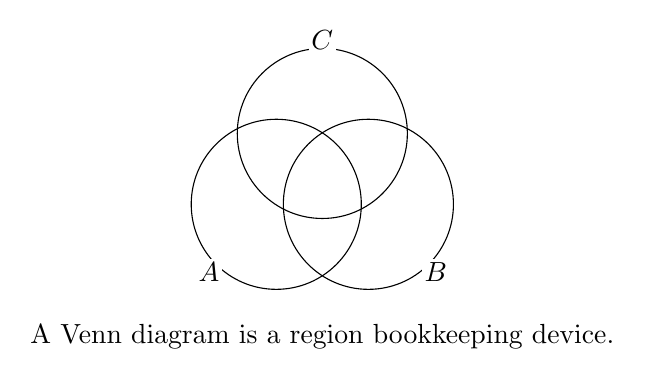
\begin{tikzpicture}[scale=0.9,every node/.style={fill=white,inner sep=1pt}]
  \draw (0,0) circle (1.2);
  \draw (1.3,0) circle (1.2);
  \draw (0.65,1.0) circle (1.2);
  \node at (-0.95,-0.95) {$A$};
  \node at (2.25,-0.95) {$B$};
  \node at (0.65,2.32) {$C$};
  \node[below] at (0.65,-1.65) {A Venn diagram is a region bookkeeping device.};
\end{tikzpicture}
\caption{For three sets one should reason region by region, not by visual guesswork alone.}
\end{figure}

\section{Difference identities}

One useful identity appearing in the handwritten reasoning is
\[
  B-C=B\cap C^c.
\]
Therefore
\[
  B-C-(A\cap B)
  =
  B\cap C^c\cap(A\cap B)^c.
\]
Using De Morgan,
\[
  (A\cap B)^c=A^c\cup B^c,
\]
so
\[
  B\cap C^c\cap(A^c\cup B^c)
  =
  (B\cap C^c\cap A^c)\cup(B\cap C^c\cap B^c).
\]
The second term is empty, hence
\[
  B-C-(A\cap B)=B\cap A^c\cap C^c.
\]
This is exactly the kind of algebraic cleanup that a Venn diagram suggests but does not replace.

\section{Coordinate and algebraic exercises}

The later pages contain a mixture of algebraic and coordinate exercises.  They include problems about quadratic expressions, tangent or chord diagrams, and conditions that must be translated into equations.  The handwritten computations repeatedly use the same pattern:
\begin{enumerate}[(i)]
  \item introduce the unknowns explicitly;
  \item translate each condition into an equation or inequality;
  \item reduce by substitution or by completing the square;
  \item check equality or boundary cases.

\end{enumerate}

Several sketches show lines touching curves or intersecting regions.  Rather than reproducing them as raw images, the important content is the method: a picture tells us which algebraic condition to impose, such as tangency, parallelism, or containment.

\section{A note on proof writing}

The red handwritten reflection says that a purely diagrammatic method is intuitive but can be unreliable.  The mature solution uses the diagram to discover the statement, then uses set algebra to prove it.  This is an excellent general lesson.  Geometry and diagrams are for finding the path; formal manipulations are for making the path safe.


\section{Extremal set problems: why constructions matter}

In an extremal counting problem, an upper bound is only half the solution.  One must also give a construction showing the bound is sharp.  The note's sum-set and difference-set arguments follow this pattern: first prove that the derived sets must contain enough elements; then exhibit a set \(A\) for which the lower bound is actually attained.

This is a common combinatorial habit.  Inequalities show impossibility beyond a threshold.  Constructions show that the threshold is real.

\section{Venn diagrams versus proofs}

Venn diagrams are excellent for discovering set identities, but the proof should eventually be written elementwise.  For example,
\[
  A\setminus(B\cup C)=(A\setminus B)\cap(A\setminus C)
\]
is proved by taking an arbitrary \(x\) and translating membership:
\[
  x\in A\setminus(B\cup C)
  \Longleftrightarrow
  x\in A,\ x\notin B,\ x\notin C.
\]
This is exactly the condition for membership in the right-hand side.  The diagram gives intuition; the element chase gives proof.

\section{Expanded synthesis and advanced context}

This note is about extremal and logical reasoning.  The extremal problem uses auxiliary sets and cardinality bounds.  The Venn problem uses Boolean algebra and region decomposition.  Both are early forms of a common method: replace a vague configuration by a finite list of regions or quantities that can be counted exactly.  This is the same spirit behind combinatorial proofs, measure decompositions, and even sigma-algebra calculations later in analysis.



\paragraph{Expanded synthesis.}
The elementary geometric content of this chapter should be read through transformations and invariants. The earlier sections (`A set construction problem`, `What this problem teaches`, `A Venn-diagram necessary-and-sufficient problem`, `Difference identities`, `Coordinate and algebraic exercises`) may use coordinates, angles, determinants, parametrizations, or integral formulas, but the organizing question is: which quantities survive the transformations naturally associated with the problem? Euclidean geometry preserves distances and angles; affine geometry preserves lines and ratios on a line; projective geometry preserves incidence and cross ratio; differential geometry preserves coordinate-independent objects such as forms, metrics, and orientations.

This perspective separates different layers of a problem. A dot product belongs to metric geometry. A determinant belongs to oriented volume. A cross ratio belongs to projective geometry. A line or surface integral of a differential form belongs to oriented topology. A scalar area integral belongs to the metric-induced measure. Confusing these layers is the source of many errors, especially in vector calculus where $dS$, $F\cdot n\,dS$, $dx\wedge dy$, and boundary orientation look similar but encode different structures.

When returning to the original examples, identify the natural object before computing. If the problem is about concurrence or collinearity, projective or affine tools may be natural. If it is about distance, angle, or orthogonality, metric tools are essential. If it is about flux or circulation, differential forms and orientation explain the signs. The advanced viewpoint makes the elementary solution more disciplined rather than more abstract for its own sake.


\section{Elementary-to-advanced bridge: extremal set theory}

The original extremal set exercises ask how large a family of sets can be under some forbidden configuration.  This is the central form of extremal combinatorics.  A typical question is: among all families $\mathcal F\subseteq \mathcal P([n])$ satisfying a condition, maximize $|\mathcal F|$.

One famous theorem is Sperner's theorem.  If $\mathcal F$ is an antichain, meaning no member contains another, then
\[
  |\mathcal F|\le \binom{n}{\lfloor n/2\rfloor}.
\]
The largest antichain is the middle layer of the Boolean lattice.

This is the advanced version of the elementary strategy ``look at the largest level.''  The theorem says that this intuition is exactly right under the antichain constraint.

\section{Elementary-to-advanced bridge: Erdős--Ko--Rado flavor}

Another central theme is intersecting families.  A family $\mathcal F\subseteq \binom{[n]}k$ is intersecting if
\[
  A\cap B\ne\varnothing
\]
for all $A,B\in\mathcal F$.  The Erdős--Ko--Rado theorem says that if $n\ge2k$, then
\[
  |\mathcal F|\le \binom{n-1}{k-1}.
\]
The extremal example is a star: all $k$-sets containing a fixed element.

This theorem explains a common pattern in elementary problems: when every pair must intersect, the largest construction often comes from forcing one common element.

\section{Elementary-to-advanced bridge: shifting and compression}

Shifting is a method that transforms a set family into a more ordered family without changing its size or destroying the required property.  A basic shift replaces an element $j$ by a smaller element $i$ when possible.  Repeated shifts push a family toward lexicographically simpler sets.

The key idea is that extremal families can often be assumed to have a compressed form.  This turns a chaotic search over all families into a structured search over monotone or shifted families.

This is the advanced form of an elementary simplification habit: if a problem is symmetric, move examples toward a canonical position.

\section{Elementary-to-advanced bridge: VC dimension}

A set family $\mathcal F\subseteq \mathcal P(X)$ shatters a subset $S\subseteq X$ if every subset of $S$ occurs as an intersection $F\cap S$ for some $F\in\mathcal F$.  The VC dimension is the largest size of a shattered set.

The Sauer--Shelah lemma says that if the VC dimension is $d$, then
\[
  |\mathcal F|\le \sum_{i=0}^d \binom ni
\]
for $|X|=n$.  Thus a local shattering restriction gives a global counting bound.

This connects elementary extremal set problems to statistical learning theory: VC dimension measures the capacity of a class of classifiers.

% Second-pass deepening for waves 2-4: wave 3 A-C part 1
\section{Second-pass deepening: extremal examples as stability problems}

An extremal theorem does not only ask for the maximum size; it also asks what near-maximum examples look like.  For Sperner's theorem, the exact extremal family is the middle layer.  A stability version asks: if an antichain has size close to
\[
  \binom n{\lfloor n/2\rfloor},
\]
must it be structurally close to the middle layer?

This is a research-level refinement of an elementary habit: after finding equality cases, ask what happens when equality is almost achieved.  Stability results are important because many real configurations are approximate rather than exact.

\section{Second-pass deepening: shifting as canonicalization}

Shifting operations preserve size and the forbidden-intersection property while simplifying the family.  After repeated shifts, if a set contains a large element but not a smaller one, the shifted family tends to replace the large element by the smaller one.

The benefit is that compressed families are easier to classify.  This is analogous to row reduction in linear algebra: one transforms an object without changing the key invariant until it has a canonical or nearly canonical form.

The original extremal exercises should therefore be expanded not only with the final theorem, but with the method: transform the family, preserve the condition, and force a structured extremal example.

\notechapter{N-20221209}{Set-Theoretic and Combinatorial Exercises after the First Lecture}

\section{What this page is doing}

This note is a handwritten exercise continuation of the set-and-counting lecture.  The problems involve floor functions, set-builder notation, binomial identities, lattice or coordinate sets, and counting arguments.  The common goal is to learn how to translate a compact set expression into something countable.

\section{A floor-function example}

One example asks for a set defined by inequalities and floor functions.  The handwritten solution separates the problem into intervals because
\[
  \lfloor x\rfloor=k\quad\Longleftrightarrow\quad k\le x<k+1.
\]
This is the essential method.  Any problem involving \(\lfloor x\rfloor\) should first be split into integer strips.

For instance, if a condition contains
\[
  3\lfloor x\rfloor-5<0,
\]
then
\[
  \lfloor x\rfloor<\frac53,
\]
so
\[
  \lfloor x\rfloor\le1.
\]
One then intersects this with the remaining condition, such as a quadratic inequality.  The final answer is an interval or a finite union of intervals.

\section{A binomial counting identity}

Another exercise invokes the binomial theorem.  The handwritten note uses the idea that terms in a sum can be counted by choosing which positions have a particular property.  A typical identity is
\[
  \sum_{j=0}^n\binom nj=2^n,
\]
or, with signs,
\[
  \sum_{j=0}^n(-1)^j\binom nj=0.
\]

The important thought is not the formula alone.  The coefficient \(\binom nj\) counts ways of choosing \(j\) positions among \(n\), and the binomial theorem packages all choices simultaneously.

\section{Solving a system by discriminants}

One problem gives a two-variable system whose equations can be transformed into a quadratic with a parameter \(p\).  The handwritten solution examines the discriminant
\[
  \Delta\ge0
\]
to decide when real solutions exist.

This is a recurring analytic-algebraic pattern: if a system can be reduced to a quadratic equation, existence of real solutions is controlled by the discriminant.  The solution set changes when the discriminant becomes zero; this is the boundary between two real roots and no real roots.

\section{A prime-number exercise}

Another exercise involves primes \(p,q\).  The handwritten reasoning uses parity and basic divisibility.  The standard approach is:
\begin{enumerate}[(i)]
  \item reduce the equation modulo a small integer such as \(2,3,4\);
  \item use the fact that the only even prime is \(2\);
  \item separate small exceptional cases before treating odd primes.

\end{enumerate}

This is the same habit developed in earlier divisibility notes: do not solve a Diophantine equation blindly.  First use congruences to force the shape of the variables.

\section{A nested-set exercise}

The note includes a Russian sentence asking to ``describe the next set'' or ``write the following set in ordinary language.''  The examples involve finite sets such as
\[
  \varnothing,\qquad \{a_1\},\qquad \{a_1,a_2\},\qquad\ldots
\]
and collections of subsets.  The intended lesson is the difference between an element and a subset:
\[
  a\in A\quad\text{versus}\quad \{a\}\subseteq A.
\]
Confusing these two is one of the most common early set-theory mistakes.

\section{A recurrence of sets}

One exercise defines sets recursively, for example
\[
  A_{k+1}=A_k\cup\{x_{k+1}\}
\]
or by adding all new subsets involving a new element.  The handwritten solution proves the pattern by induction: assume the formula for \(A_k\), then show the construction gives \(A_{k+1}\).

This is the set-theoretic analogue of a recurrence relation.  Instead of numbers changing with \(k\), collections of objects change with \(k\).

\section{An intersection-counting problem}

The final exercise on the second page asks whether a selected element belongs to an intersection of many sets.  The handwritten solution builds sets \(B(A_i)\) and counts their sizes, arriving at a large product-like number.  The exact numerical expression is less important than the logic:
\begin{enumerate}[(i)]
  \item translate membership into a condition;
  \item count how many sets contain a fixed element;
  \item use complements or intersections to isolate the desired elements.

\end{enumerate}
This is a typical finite-set counting method: count incidence pairs in two ways.


\section{Set-builder notation as a translation problem}

A complicated set-builder expression should be read in stages.  First identify the universe of discourse.  Then translate each condition into an inequality, divisibility condition, or membership condition.  Finally decide whether the problem is asking for the set itself, its size, or a proof of equality.

For example, a condition involving \(\lfloor x\rfloor\) is not smooth; it divides the real line into half-open intervals.  A condition involving binomial coefficients often asks for a counting interpretation rather than algebraic simplification.

\section{Recursive set construction}

When a set is defined recursively, the first few stages should be computed explicitly.  This reveals whether the construction is increasing, periodic, stabilizing, or producing genuinely new elements.  After that, induction is the natural proof method.

The general pattern is:
\[
  S_0\subseteq S_1\subseteq S_2\subseteq\cdots
\]
if the rule is monotone.  If the universe is finite, an increasing chain must eventually stabilize.  This is a useful idea behind many finite combinatorial processes.

\section{Expanded synthesis and advanced context}

The exercises are elementary, but they are training the language of discrete mathematics.  Floor functions partition the real line into strips; binomial coefficients count choices; discriminants detect existence; recursive set definitions invite induction; incidence counting turns membership questions into arithmetic.  The high-level skill is always the same: replace notation by a structure that can actually be counted.



\paragraph{Expanded synthesis.}
For this chapter, the elementary material should be read as a study of what remains invariant when coordinates change. The earlier sections (`What this page is doing`, `A floor-function example`, `A binomial counting identity`, `Solving a system by discriminants`, `A prime-number exercise`) compute with arrays, bases, pivots, determinants, or eigenvectors; the deeper object is a linear map together with the spaces it acts on. A matrix is a representation of that map after bases have been chosen. This is why formulas such as
\[
  A' = P^{-1}AP,\qquad \widetilde A = T^{-1}AS
\]
are not cosmetic: they distinguish an intrinsic morphism from a coordinate description.

The structural hierarchy is as follows. Kernels record what a map forgets, images record what it reaches, cokernels record obstructions to solvability, and quotients record information after an equivalence has been imposed. Determinants act on the top exterior power and therefore measure oriented volume; traces are invariant under cyclic rearrangement and become characters in representation theory; adjoints depend on an inner product and lead to self-adjoint spectral theory.

A useful way to return to the computations is to ask, for every formula, which invariant it is measuring. Row reduction measures rank and kernel; diagonalization measures decomposition into invariant subspaces; Gram--Schmidt measures orthogonal projection; positive definiteness measures ellipsoid geometry; tensor notation measures how components transform. The elementary methods are therefore the finite-dimensional laboratory in which duality, quotienting, functoriality, and spectral decomposition can be seen clearly.


\section{Elementary-to-advanced bridge: finite differences and polynomial degree}

Many binomial and floor-sum exercises can be clarified by finite differences.  For a sequence $a(n)$, define
\[
  \Delta a(n)=a(n+1)-a(n).
\]
If $a(n)$ is a polynomial of degree $d$, then $\Delta a(n)$ has degree $d-1$, and
\[
  \Delta^{d+1}a(n)=0.
\]
This is the discrete analogue of differentiating a polynomial until it vanishes.

The binomial coefficient basis is especially natural:
\[
  \Delta \binom nk=\binom n{k-1}.
\]
Therefore integer-valued polynomials are naturally expanded in the basis
\[
  \binom n0,\ \binom n1,\ \binom n2,\ \ldots.
\]

This explains why binomial sums repeatedly appear in discrete counting problems: they are the coordinate system in which finite difference is simplest.

\section{Elementary-to-advanced bridge: polynomial method}

The polynomial method proves combinatorial statements by constructing a polynomial with too many roots or with controlled degree.  The elementary fact is: a nonzero polynomial of degree $d$ over a field has at most $d$ roots.  In several variables, one uses more refined versions involving degree and vanishing on grids.

For example, if a polynomial $P(x)$ of degree at most $n-1$ vanishes at $n$ distinct points, then $P=0$.  Lagrange interpolation gives the exact reconstruction formula:
\[
  P(x)=\sum_{i=1}^n P(a_i)\prod_{j\ne i}\frac{x-a_j}{a_i-a_j}.
\]
Counting information can therefore be encoded into polynomial values.

This is a research-level extension of elementary identities: prove a combinatorial impossibility by forcing a polynomial to be zero while one coefficient or value remains nonzero.

\section{Elementary-to-advanced bridge: Burnside's lemma}

When the note counts objects with symmetry, the advanced principle is group action.  If a finite group $G$ acts on a finite set $X$, the number of orbits is
\[
  |X/G|=\frac1{|G|}\sum_{g\in G}|\operatorname{Fix}(g)|.
\]
This is Burnside's lemma.

It explains why counting up to rotation or reflection requires averaging fixed points rather than simply dividing by the number of symmetries.  Some objects have nontrivial stabilizers, so not every orbit has the same size.

\section{Returning to the original exercises}

Floor sums, binomial identities, and symmetry counts are not separate genres.  Finite differences handle discrete polynomial behavior; the polynomial method turns combinatorics into algebra; group actions handle symmetry.  These are three advanced continuations of the elementary counting toolkit.

% Second-pass deepening for waves 2-4: wave 3 A-C part 1
\section{Second-pass deepening: floor functions as lattice-point counts}

A floor expression such as
\[
  \left\lfloor \frac{an+b}{m}\right\rfloor
\]
counts how many integer thresholds have been crossed.  Sums of floor functions often count lattice points below a line.  For example,
\[
  \sum_{k=0}^{m-1}\left\lfloor \frac{ak}{m}\right\rfloor
\]
counts integer points under a rational-slope diagonal in a rectangle.

This links elementary floor identities to Ehrhart theory, where one counts lattice points in dilates of polytopes:
\[
  L_P(n)=|nP\cap\mathbb Z^d|.
\]
For integral polytopes, $L_P(n)$ is a polynomial in $n$.  Thus floor-sum exercises are one-dimensional shadows of lattice-point enumeration.

\section{Second-pass deepening: group actions as corrected division}

When counting objects up to symmetry, naive division by $|G|$ fails if some objects have symmetry.  Burnside's lemma repairs this by averaging fixed points.  This idea should be tied back to elementary examples: necklaces, colorings of polygons, and arrangements under rotation/reflection.

The orbit-stabilizer theorem explains the correction:
\[
  |Gx|=\frac{|G|}{|\operatorname{Stab}(x)|}.
\]
Objects with larger stabilizers have smaller orbits and must be weighted correctly.  This is why symmetry counting is more subtle than ordinary counting.

\notechapter{N-20221210}{Binomial Theorem, Absolute-Value Estimates, and Set Exercises}

\section{Binomial theorem}

The first page begins with the binomial theorem:
\[
  (a+b)^n=\sum_{i=0}^n \binom ni a^i b^{n-i}.
\]
The handwritten derivation emphasizes selection.  When expanding
\[
  (a+b)(a+b)\cdots(a+b),
\]
one chooses either $a$ or $b$ from each factor.  A term $a^ib^{n-i}$ occurs when $a$ is chosen from exactly $i$ of the $n$ factors, and this can be done in $\binom ni$ ways.

The same idea proves the recurrence
\[
  \binom{n+1}{i}=\binom ni+\binom n{i-1},
\]
because in choosing $i$ objects from $n+1$, either the new object is not chosen or it is chosen.

\section{Absolute value of binomial sums}

The note then estimates expressions such as
\[
  |a+b|^n.
\]
Using the triangle inequality and the binomial theorem,
\[
  |a+b|^n
  \le (|a|+|b|)^n
  =\sum_{i=0}^n \binom ni |a|^i|b|^{n-i}.
\]
The important habit is to move absolute values inside after expanding only when one has a legitimate inequality.  The handwritten page marks the triangle inequality as the justification.

\section{A summation exercise}

One exercise asks for a sum of the form
\[
  \sum_{i=0}^n \binom ni.
\]
Putting $a=b=1$ in the binomial theorem gives
\[
  2^n=\sum_{i=0}^n \binom ni.
\]
Similarly, putting $a=1,b=-1$ gives
\[
  0=(1-1)^n=\sum_{i=0}^n (-1)^{n-i}\binom ni,
\]
which shows that the sum of even-indexed binomial coefficients equals the sum of odd-indexed ones when $n>0$.

\section{Set exercises}

The printed pages list elementary set exercises.  The notes use standard notation:
\[
  A\cup B,\qquad A\cap B,\qquad A\setminus B,\qquad A^c.
\]
One recurring task is to translate a verbal condition into set operations.  For example,
\[
  A\setminus(B\cup C)=(A\setminus B)\cap(A\setminus C).
\]
This is proved elementwise:
\[
  x\in A\setminus(B\cup C)
  \Longleftrightarrow
  x\in A,\ x\notin B,\ x\notin C.
\]

The exercises also ask for necessary and sufficient conditions for equalities such as
\[
  A\cup B=A,\qquad A\cap B=B.
\]
Both are equivalent to
\[
  B\subseteq A.
\]

\section{Counting subsets with properties}

For a finite set $X$ with $|X|=n$, the number of subsets is
\[
  2^n.
\]
If one imposes parity conditions, the count is often half of the total.  For example, the number of subsets of an $n$-element set with even cardinality is
\[
  2^{n-1},
\]
when $n\ge1$.  This follows from
\[
  \sum_{k\text{ even}}\binom nk
  =
  \sum_{k\text{ odd}}\binom nk
  =2^{n-1}.
\]

The printed exercises include conditions involving positive and negative numbers, odd and even elements, and sums of elements.  The general method is to split the set into independent categories and multiply the numbers of choices.

\section{Set-builder notation}

The note also works with sets such as
\[
  U=\{x:x=2n,\ n\in\mathbb Z\},\qquad
  V=\{x:x=3n,\ n\in\mathbb Z\}.
\]
Here $U$ is the set of even integers and $V$ is the set of multiples of $3$.  Then
\[
  U\cap V=\{x:x=6n,\ n\in\mathbb Z\}
\]
and
\[
  U\cup V
\]
is the set of integers divisible by $2$ or by $3$.

The point is to read set-builder notation as a logical predicate.

\section{Expanded synthesis and advanced context}

The note links binomial coefficients with set counting.  The binomial theorem counts choices from factors; subset counting counts choices from elements.  The same coefficients $\binom nk$ appear in both languages.  Set identities should be proved elementwise, while counting identities should be proved by telling a story about what is being chosen.



\paragraph{Expanded synthesis.}
The elementary geometric content of this chapter should be read through transformations and invariants. The earlier sections (`Binomial theorem`, `Absolute value of binomial sums`, `A summation exercise`, `Set exercises`, `Counting subsets with properties`) may use coordinates, angles, determinants, parametrizations, or integral formulas, but the organizing question is: which quantities survive the transformations naturally associated with the problem? Euclidean geometry preserves distances and angles; affine geometry preserves lines and ratios on a line; projective geometry preserves incidence and cross ratio; differential geometry preserves coordinate-independent objects such as forms, metrics, and orientations.

This perspective separates different layers of a problem. A dot product belongs to metric geometry. A determinant belongs to oriented volume. A cross ratio belongs to projective geometry. A line or surface integral of a differential form belongs to oriented topology. A scalar area integral belongs to the metric-induced measure. Confusing these layers is the source of many errors, especially in vector calculus where $dS$, $F\cdot n\,dS$, $dx\wedge dy$, and boundary orientation look similar but encode different structures.

When returning to the original examples, identify the natural object before computing. If the problem is about concurrence or collinearity, projective or affine tools may be natural. If it is about distance, angle, or orthogonality, metric tools are essential. If it is about flux or circulation, differential forms and orientation explain the signs. The advanced viewpoint makes the elementary solution more disciplined rather than more abstract for its own sake.


\section{Elementary-to-advanced bridge: binomial transform}

The binomial theorem gives
\[
  (1+x)^n=\sum_{k=0}^n \binom nk x^k.
\]
The binomial transform of a sequence $(a_k)$ is
\[
  b_n=\sum_{k=0}^n \binom nk a_k.
\]
It has an inverse:
\[
  a_n=\sum_{k=0}^n (-1)^{n-k}\binom nk b_k.
\]
This is Möbius inversion on the subset lattice in sequence form.

Thus binomial identities in the note can often be read as transformations between two coordinate systems for sequences.

\section{Elementary-to-advanced bridge: exponential generating functions and labelled structures}

For labelled combinatorial structures, the exponential generating function is
\[
  A(x)=\sum_{n\ge0}a_n\frac{x^n}{n!}.
\]
The factor $n!$ compensates for labellings.  Products of exponential generating functions correspond to splitting a labelled set into labelled parts.

For example, the exponential formula says that if a structure is a set of connected components, then its exponential generating function is the exponential of the generating function for connected components:
\[
  A(x)=\exp(C(x)).
\]
This is the advanced version of the elementary idea that a set can be decomposed into independent pieces.

\section{Elementary-to-advanced bridge: combinatorial species}

A combinatorial species is a functor from finite sets with bijections to finite sets of structures.  For each finite label set $U$, a species $F$ assigns a set $F[U]$ of structures on $U$; every bijection $U\to V$ transports structures from $F[U]$ to $F[V]$.

This functorial language records not only how many objects exist, but how they behave under relabelling.  The binomial theorem corresponds to the species identity for subsets: choosing a subset of an $n$-set means splitting labels into chosen and unchosen parts.

\section[Probability view of binomial coefficients]{Elementary-to-advanced bridge: probability distributions behind binomial coefficients}

The binomial coefficients also appear in probability.  If $X\sim \operatorname{Bin}(n,p)$, then
\[
  \mathbb P(X=k)=\binom nk p^k(1-p)^{n-k}.
\]
The binomial theorem ensures total probability equals $1$:
\[
  \sum_{k=0}^n\binom nk p^k(1-p)^{n-k}=1.
\]
The generating function is
\[
  \mathbb E[t^X]=(1-p+pt)^n.
\]
Thus binomial algebra, subset counting, and sums of independent Bernoulli random variables are the same structure.

% Second-pass deepening for waves 2-4: wave 3 A-C part 1
\section{Second-pass deepening: binomial identities as change of basis}

The polynomials
\[
  \binom x0,\ \binom x1,\ \binom x2,\ldots
\]
form a natural basis for polynomial functions on integers.  The finite difference operator acts simply:
\[
  \Delta \binom xk=\binom x{k-1}.
\]
Therefore many binomial identities are not coincidences; they are coordinate transformations in this basis.

For example, Vandermonde's identity
\[
  \sum_k \binom rk\binom s{n-k}=\binom{r+s}n
\]
is coefficient extraction from
\[
  (1+x)^r(1+x)^s=(1+x)^{r+s}.
\]
It also counts choosing $n$ elements from a disjoint union of sets of sizes $r$ and $s$.

\section{Second-pass deepening: species and the meaning of labels}

In labelled counting, the labels matter only up to bijection.  A species formalizes this by requiring every bijection of label sets to transport structures.  This turns counting into functorial combinatorics.

For instance, the species of subsets assigns to a finite set $U$ the set $\mathcal P(U)$.  A bijection $U\to V$ sends a subset of $U$ to the corresponding subset of $V$.  The binomial theorem is the decategorified shadow of this functorial behavior.

\notechapter{N-20230118}{Combinatorics: Pigeonhole Principle, Subsets, Binomial Sums, and Helly-Type Ideas}

\section{Pigeonhole principle}

The note begins with the pigeonhole principle.  If $n+1$ objects are put into $n$ boxes, then some box contains at least two objects.  More generally, if $N$ objects are placed into $k$ boxes, then some box contains at least
\[
  \left\lceil \frac Nk \right\rceil
\]
objects.

The handwritten examples use this principle to force coincidences: same remainder, same subset size, same color, or same interval.  The key is to decide what the boxes are.  Often the boxes are congruence classes modulo $m$ or possible values of a sum.

\section{Subsets and binomial coefficients}

For $[n]=\{1,2,\ldots,n\}$, the number of $k$-element subsets is
\[
  \binom nk.
\]
The note uses the identity
\[
  \sum_{k=0}^n \binom nk=2^n
\]
to count all subsets.  It also uses
\[
  \sum_{k=0}^n k\binom nk=n2^{n-1}.
\]
This identity counts pairs $(A,a)$ where $A\subseteq[n]$ and $a\in A$.  Choose $a$ first in $n$ ways, then choose the rest of $A$ freely in $2^{n-1}$ ways.

\section{Binomial identities by double counting}

The handwritten page contains identities of the type
\[
  \sum_j \binom aj\binom b{n-j}=\binom{a+b}{n}.
\]
This is Vandermonde's identity.  The combinatorial proof is to choose $n$ objects from two groups of sizes $a$ and $b$.  If $j$ objects are chosen from the first group, then $n-j$ are chosen from the second.

The note marks this as a better proof than manipulating factorials, because it explains why the identity is true.

\section{A subset-sum style example}

One example lists several subsets $A_i$ of a finite set and asks for a conclusion about intersections or unions.  The general method is to encode each element by the list of sets containing it.  If there are too many subsets or too many incidences, two elements must share a pattern, or some intersection must be nonempty.

This is a typical pigeonhole principle application: the objects are elements or subsets, and the boxes are possible membership patterns.

\section{Generating functions}

The page also uses generating functions for binomial sums.  The coefficient of $x^r$ in
\[
  (1+x)^n
\]
is $\binom nr$.  The coefficient of $x^r$ in
\[
  (1+x)^a(1+x)^b=(1+x)^{a+b}
\]
gives Vandermonde's identity.

This is the algebraic version of double counting.  The combinatorial story and the generating-function coefficient extraction are two descriptions of the same structure.

\section{Helly-type remark}

The last page mentions Helly's theorem.  In the plane, Helly's theorem says that for a finite family of convex sets, if every three of them have nonempty intersection, then the whole family has nonempty intersection.  The note does not prove the full theorem, but it points toward the idea that local intersection data can force global intersection.

This belongs naturally after the pigeonhole and subset examples: it is another local-to-global principle, now in convex geometry rather than finite counting.

\section{Expanded synthesis and advanced context}

The note is about forcing structure from too many objects and too few possibilities.  The pigeonhole principle forces repetition.  Binomial coefficients count choices.  Double counting proves identities by counting the same set twice.  Generating functions package these identities algebraically.  Helly-type theorems show that similar local-to-global principles also appear in geometry.



\paragraph{Expanded synthesis.}
The higher-level content of this chapter is the passage from pointwise description to invariant structure. The earlier sections (`Pigeonhole principle`, `Subsets and binomial coefficients`, `Binomial identities by double counting`, `A subset-sum style example`, `Generating functions`) introduce objects that may be drawn, listed, glued, or computed, but the advanced question is what remains unchanged under the allowed maps. In topology the allowed maps are continuous maps; in category theory they are morphisms preserving the relevant structure; in homology they induce maps between algebraic invariants.

The guiding pattern is
\[
  \text{space or structure}\quad \xrightarrow{\text{allowed maps}}\quad \text{invariant data}.
\]
Quotient spaces formalize gluing; products formalize simultaneous coordinates; compactness formalizes the impossibility of escaping by a limiting process; connectedness formalizes the impossibility of separation; homology converts holes into groups. When a note discusses closure, quotienting, paths, products, or functors, it is already working with this invariant language.

A quotient exercise is a gluing construction; a compactness exercise is an infinite pigeonhole argument; a homotopy exercise is a controlled deformation; a functorial example says that a construction is compatible with maps. The advanced theory does not add decoration. It explains why the same few operations, such as taking products, quotients, images, kernels, and induced maps, occur throughout topology, algebra, and geometry.


\section{Elementary-to-advanced bridge: pigeonhole as compactness principle}

The finite pigeonhole principle says that too many objects placed into too few boxes force repetition.  A compactness version says that if infinitely many points lie in a compact metric space, then some subsequence converges.  In $[0,1]$, this is Bolzano--Weierstrass.

The proof is a repeated pigeonhole argument: divide the interval into finitely many pieces, choose one containing infinitely many points, subdivide again, and continue.  The nested intervals shrink to a point.

Thus compactness is an infinite pigeonhole principle.  This is why elementary pigeonhole arguments often foreshadow topology and analysis.

\section{Elementary-to-advanced bridge: Ramsey theory}

Ramsey theory says that sufficiently large structures contain ordered substructures.  The simplest theorem is: for every $r,s$, there exists $R(r,s)$ such that every red-blue coloring of the edges of $K_{R(r,s)}$ contains either a red $K_r$ or a blue $K_s$.

The pigeonhole principle is the smallest Ramsey theorem.  It guarantees equality of colors or boxes; Ramsey theory guarantees large monochromatic patterns.

This connects elementary ``two objects must share a property'' problems with a research field studying unavoidable order inside large disorder.

\section{Elementary-to-advanced bridge: Helly theorem}

Helly's theorem in $\mathbb R^d$ says that for a finite family of convex sets, if every $d+1$ of them have nonempty intersection, then the whole family has nonempty intersection.

For $d=1$, this says that if intervals pairwise intersect, then all intervals intersect.  That case is a strong one-dimensional pigeonhole-like fact.  In higher dimensions, convexity replaces linear order.

The original Helly-type ideas are therefore not just clever geometry.  They are the finite-dimensional form of a general intersection principle.

\section{Elementary-to-advanced bridge: fractional and topological Helly}

Fractional Helly theorems weaken the condition: if a positive fraction of all small subfamilies intersect, then a large subfamily has common intersection.  Topological Helly theorems replace convexity by conditions on homology or contractibility of intersections.

This is a research-level continuation of the elementary principle: local intersection data can force global intersection.  The advanced theory asks exactly how much local data is enough and what kind of geometry can replace convexity.

% Second-pass deepening for waves 2-4: wave 3 A-C part 2
\section{Second-pass deepening: local-to-global intersection principles}

Helly's theorem is powerful because it turns local intersection data into global intersection.  In $\mathbb R^d$, checking every $d+1$ members of a finite convex family suffices.  The number $d+1$ is not arbitrary: it is the size at which affine dependence begins, by Radon's theorem.

Radon's theorem says that any $d+2$ points in $\mathbb R^d$ can be partitioned into two sets whose convex hulls intersect.  Helly's theorem can be proved from Radon's theorem.  This links elementary convex geometry to the combinatorics of affine dependence.

\section{Second-pass deepening: Ramsey as structured inevitability}

Pigeonhole says repetition is inevitable.  Ramsey says organized substructure is inevitable.  The shift from repetition to substructure is the main conceptual jump.  In graph terms, edge colorings of large complete graphs must contain large monochromatic complete subgraphs.

This point should be connected back to the original exercises: whenever an argument says ``among many objects, two must share a property,'' one can ask the Ramsey-level question, ``among sufficiently many objects, must a whole structured subset share the property?''

\notechapter{N-20240323}{Combinatorics: Identities, Generating Functions, Catalan Numbers, and More}


\section{Binomial identities}

The note opens with several binomial identities and, more importantly, their combinatorial meanings.  The basic identity
\[
  \sum_{i=0}^n \binom ni=2^n
\]
counts all subsets of an $n$-element set: choosing a subset means choosing its size $i$ and then choosing $i$ elements.

Pascal's identity
\[
  \binom ni+\binom n{i+1}=\binom{n+1}{i+1}
\]
can be proved by fixing a distinguished element in an $(n+1)$-element set.  An $(i+1)$-subset either contains the distinguished element or it does not.  The two cases give the two terms on the left.

Vandermonde's identity
\[
  \sum_i \binom mi \binom n{r-i}=\binom{m+n}{r}
\]
counts choosing $r$ balls from two boxes with $m$ and $n$ balls.  If $i$ balls are chosen from the first box, then $r-i$ are chosen from the second.

Another useful identity is
\[
  \binom nr \binom{n-r}{k-r}=\binom nk \binom kr.
\]
Both sides count a pair $(R,K)$ with $R\subseteq K\subseteq[n]$, $|R|=r$, and $|K|=k$.

\section{Good subsets}

A nonempty subset $A\subseteq\{1,2,\ldots,n\}$ is called good if
\[
  |A|\le \min_{x\in A}x.
\]
Let $a_n$ be the number of good subsets.  The problem asks one to prove
\[
  a_{n+2}=a_{n+1}+a_n+1.
\]

A clean proof splits good subsets of $[n+2]$ into cases.

First, if $n+2\notin A$, then $A$ is just a good subset of $[n+1]$, giving $a_{n+1}$ possibilities.

Second, if $A=\{n+2\}$, this gives one extra subset.

Third, suppose $n+2\in A$ and $|A|\ge2$.  Remove $n+2$ and subtract $1$ from every remaining element.  If
\[
  A'=A\setminus\{n+2\},
\]
then the condition becomes
\[
  |A'|+1\le \min A'.
\]
After shifting $B=\{x-1:x\in A'\}$, this is exactly
\[
  |B|\le \min B,
\]
so $B$ is a good subset of $[n]$.  This gives $a_n$ possibilities.  Hence
\[
  a_{n+2}=a_{n+1}+a_n+1.
\]

The handwritten page also gives a summation proof by fixing $|A|=k$.  If $|A|=k$, then every element must be at least $k$, so one chooses the remaining data from a tail interval.  The recurrence then follows by repeated Pascal identities.

\section{Generating functions}

For a sequence $(a_n)_{n\ge0}$, its ordinary generating function is
\[
  f(x)=\sum_{n\ge0}a_nx^n.
\]
The note emphasizes a key principle: coefficients can encode counting problems.

For example, the number of nonnegative integer solutions of
\[
  x_1+x_2+\cdots+x_k=n
\]
is the coefficient of $x^n$ in
\[
  (1+x+x^2+\cdots)^k=\frac1{(1-x)^k}.
\]
Using the binomial expansion,
\[
  \frac1{(1-x)^k}=\sum_{n\ge0}\binom{n+k-1}{k-1}x^n,
\]
so the number of solutions is
\[
  \binom{n+k-1}{k-1}.
\]

The notes also use generating functions to separate parity or color constraints.  A typical trick is to multiply several series, each recording the allowed choices for one box or color, and then read off the coefficient of the target power.

% N-20240323 overflow relief A
\enlargethispage{4\baselineskip}
\section{A probability example with repeated trials}

One example considers repeated trials and asks for a probability after $n$ operations.  The handwritten solution introduces a generating function and then rewrites nested binomial sums using exponentials.  The important method is not the final closed form alone but the transformation:
\[
  \text{complicated convolution}
  \quad\longrightarrow\quad
  \text{product/composition of generating functions}.
\]
This is a standard way to turn repeated independent operations into algebra.  Binomial coefficients record choices; exponential series record independent counts; coefficient extraction recovers the desired probability.

\section{Catalan numbers}

The note then turns to Catalan numbers.  One model is the number of ways to triangulate a convex $(n+2)$-gon:
\[
  C_n=\frac1{n+1}\binom{2n}{n}.
\]
For example, a hexagon has $14$ triangulations.

Let $h_n$ denote the number of triangulations of an $(n+2)$-gon.  Choose the triangle incident with a fixed side.  If its third vertex cuts the polygon into two smaller polygons, the numbers of triangulations multiply.  Therefore
\[
  h_n=\sum_{i=0}^{n-1}h_i h_{n-1-i},\qquad h_0=1.
\]
If
\[
  H(x)=\sum_{n\ge0}h_nx^n,
\]
then the recurrence gives
\[
  H(x)=1+xH(x)^2.
\]
Solving the quadratic and choosing the branch with $H(0)=1$ gives
\[
  H(x)=\frac{1-\sqrt{1-4x}}{2x},\qquad
  h_n=C_n.
\]

This derivation explains why Catalan numbers appear in triangulations, parentheses, Dyck paths, and many noncrossing structures: all of them are recursively split into a left and a right part.

\section{Convex sets and convex hulls}

The geometry part defines a convex set $S$ by the condition that for any $x,y\in S$ and any $t\in[0,1]$,
\[
  tx+(1-t)y\in S.
\]
Equivalently, $S$ contains the line segment between any two of its points.  The note contrasts convex and non-convex examples.

For finitely many points $x_1,\ldots,x_k$, their convex hull is
\[
  \left\{\sum_{i=1}^k t_ix_i:\ t_i\ge0,\ \sum_{i=1}^k t_i=1\right\}.
\]
The handwritten proof uses induction on $k$: the case $k=2$ is the definition of a segment; the induction step writes the convex combination as a combination of one point and a convex combination of the remaining points.

\section{Separating convex sets}

The note sketches a separation idea.  For two disjoint convex sets, one tries to find a point pair realizing minimal distance and then uses the perpendicular bisector of the segment between them as a separating line.  In symbols, if $u\in S_1$ and $v\in S_2$ are closest points, then the hyperplane perpendicular to $v-u$ near the midpoint separates the two sets.

In finite-dimensional Euclidean geometry, this is the intuitive core of the separating hyperplane theorem.  The handwritten diagrams show projections onto a line and inequalities involving squared distances.  The algebra expands
\[
  \|u+t(a-u)-v\|^2
\]
for small $t$ and extracts a sign condition by letting $t\to0$.

\section{Planar graphs and Euler-type counting}

The later pages move toward graph theory and planar configurations.  The recurring idea is that a planar drawing imposes counting restrictions.  Vertices, edges, and faces cannot vary independently; they are constrained by Euler-type formulas.

This connects naturally with the previous convex-geometry material: triangulations, planar graphs, polygon decompositions, and convex hulls are different languages for controlling incidence data.

\section{Graphs and adjacency matrices}

A graph $G$ consists of a vertex set $V=\{v_1,\ldots,v_n\}$ and an edge relation.  For a simple graph, the adjacency matrix $A(G)=(a_{ij})$ is defined by
\[
  a_{ij}=
  \begin{cases}
  1,&\text{if there is an edge from }v_i\text{ to }v_j,\\
  0,&\text{otherwise.}
  \end{cases}
\]
For a multigraph, $a_{ij}$ records the number of edges from $v_i$ to $v_j$.

The source quotes the standard theorem: the $(i,j)$-entry of $A(G)^\ell$ equals the number of walks of length $\ell$ from $v_i$ to $v_j$.  The proof is matrix multiplication.  For $\ell=2$,
\[
  (A^2)_{ij}=\sum_k a_{ik}a_{kj},
\]
which counts all intermediate vertices $v_k$.  The general case follows by induction.

% N-20240323 overflow relief B
\enlargethispage{4\baselineskip}
\section{Expanded synthesis and advanced context}

This note collects several ways of counting: direct binomial identities, recurrence, generating functions, Catalan decomposition, convex geometry, and graph adjacency matrices.  The common habit is to replace a raw counting problem by a structure-preserving encoding: subsets become binomial coefficients, recursions become generating functions, triangulations become Catalan recurrences, convex hulls become linear combinations, and walks become matrix powers.



\paragraph{Expanded synthesis.}
The number-theoretic content of this chapter is best understood as arithmetic seen through algebraic structure. The earlier sections (`Binomial identities`, `Good subsets`, `Generating functions`, `A probability example with repeated trials`, `Catalan numbers`) compute divisibility, congruences, residues, prime factorizations, or finite-field examples. The deeper language is ideals, quotient rings, unit groups, valuations, and field extensions.

Divisibility in $\mathbb Z$ is containment of principal ideals; congruence modulo $n$ is equality inside the quotient ring $\mathbb Z/n\mathbb Z$; invertibility modulo $n$ means being a unit; the Chinese remainder theorem is a product decomposition of quotient rings. Prime factorization supplies coordinates through valuations:
\[
  n=\prod_p p^{v_p(n)}.
\]
Gcd and lcm are coordinatewise minimum and maximum in these valuation coordinates.

This algebraic reading explains why elementary tricks scale upward. Euclidean algorithms become the theory of Euclidean domains and PIDs; divisor sums become Dirichlet convolution and Euler products; roots of unity become cyclotomic fields and Galois actions; finite polynomial arithmetic becomes finite-field theory. The original computations should therefore be kept as the algorithmic core, while the advanced language identifies the structure that makes the algorithms work.


\section{Elementary-to-advanced bridge: Catalan numbers as recursive geometry}

Catalan numbers count many objects: correctly matched parentheses, triangulations of polygons, rooted binary trees, Dyck paths, and noncrossing partitions.  A standard formula is
\[
  C_n=\frac1{n+1}\binom{2n}{n}.
\]
The recursion
\[
  C_{n+1}=\sum_{i=0}^n C_iC_{n-i}
\]
comes from choosing the first return of a Dyck path or the root split of a binary tree.

The generating function $C(x)=\sum_{n\ge0}C_nx^n$ satisfies
\[
  C(x)=1+xC(x)^2.
\]
Solving gives
\[
  C(x)=\frac{1-\sqrt{1-4x}}{2x}.
\]
Thus an elementary recursion becomes an algebraic generating function.

\section{Elementary-to-advanced bridge: lattice paths and reflection principle}

Many Catalan formulas are proved by the reflection principle.  The number of paths from $(0,0)$ to $(n,n)$ that never go above the diagonal is
\[
  \binom{2n}{n}-\binom{2n}{n+1}=\frac1{n+1}\binom{2n}{n}.
\]
The subtracted term counts bad paths by reflecting the part up to the first diagonal crossing.

This is a model example of an involutive or bijective proof.  Rather than evaluating a sum, one constructs a symmetry pairing bad objects with easier objects.

\section{Elementary-to-advanced bridge: graph walks and adjacency matrices}

If $G$ is a finite graph with adjacency matrix $A$, then
\[
  (A^k)_{ij}
\]
counts walks of length $k$ from vertex $i$ to vertex $j$.  This turns walk counting into matrix powers.

If $A$ is diagonalizable with eigenvalues $\lambda_1,\ldots,\lambda_n$, the growth of walks is controlled by the largest eigenvalues.  In a regular connected graph, the largest eigenvalue is the degree, and the second-largest eigenvalue controls expansion and mixing.

Thus an elementary graph-walk count leads directly to spectral graph theory.

\section{Elementary-to-advanced bridge: random walks and Markov chains}

Normalize the adjacency matrix of a $d$-regular graph by
\[
  P=\frac1d A.
\]
Then $P$ is the transition matrix of a random walk.  The distribution after $k$ steps is
\[
  \pi_k=\pi_0P^k.
\]
Eigenvalues of $P$ determine convergence to stationarity.  If the graph is connected and non-bipartite, the walk converges to the uniform distribution.

The same object therefore has two readings: $A^k$ counts deterministic walks, while $P^k$ describes probabilities.  The note's graph-walk calculations are the finite beginning of Markov-chain theory.

% Second-pass deepening for waves 2-4: wave 3 A-C part 2
\section{Second-pass deepening: Catalan recursion and moduli of parenthesization}

Polygon triangulations and parenthesizations are the same combinatorial structure.  A triangulation of an $(n+2)$-gon corresponds to a way of multiplying $n+1$ factors with binary parentheses.  Choosing the triangle incident to a fixed edge splits the polygon into two smaller polygons, producing the Catalan recursion.

This is the combinatorics behind the associahedron, a polytope whose vertices are parenthesizations and whose edges are single reassociations:
\[
  (ab)c\leftrightarrow a(bc).
\]
The elementary Catalan count therefore touches the geometry of moduli spaces of bracketings.

\section{Second-pass deepening: adjacency spectra and expansion}

The theorem that $(A^k)_{ij}$ counts walks becomes much stronger when combined with eigenvalues.  If a graph is $d$-regular with adjacency eigenvalues
\[
  d=\lambda_1\ge |\lambda_2|\ge\cdots,
\]
then $|\lambda_2|$ controls how quickly random walks mix and how well the graph expands.

Expander graphs are sparse graphs that behave like highly connected graphs.  They are central in theoretical computer science, coding theory, and combinatorics.  The elementary walk-counting matrix is the first tool for studying them.

\notechapter{N-20240330}{Combinatorial Geometry, Euler Formula, Platonic Solids, Degree, and Quotients}

\section{Good triangles}

The first problem concerns $n$ points in the plane with no three collinear.  A triangle formed by three of these points is called good if its area is maximal among all triangles formed by the point set.  The goal is to show that there cannot be more than $n$ good triangles.

The note begins with small cases.  For $n=4$, a convex quadrilateral gives four good-looking candidate triangles by deleting one vertex.  For $n=5$, a pentagon suggests five candidates.  These pictures motivate the expected upper bound.

\section{Why vertices must lie on the convex hull}

If a triangle uses a point strictly inside the convex hull, it cannot be maximal.  Moving that interior vertex outward toward a hull vertex while keeping the opposite side fixed increases area.  Therefore every good triangle has all three vertices on the boundary of the convex hull.

This is the first reduction: the problem becomes cyclic.  We may list the hull vertices in clockwise order and encode a triangle by the three arc lengths between its consecutive vertices.

\section{Cyclic arc encoding}

Let a good triangle have vertices $A,B,C$ on the convex hull, ordered cyclically.  Let
\[
  a,b,c
\]
be the numbers of boundary steps along the three arcs from $A$ to $B$, from $B$ to $C$, and from $C$ back to $A$.  Then
\[
  a+b+c=m,
\]
where $m$ is the number of hull vertices.

The handwritten argument tries to order all good triangles by their arc data.  If one arc is too large compared with another, then shifting a vertex along the circle or convex boundary can produce a triangle of larger area, contradicting maximality.  The intended conclusion is that good triangles are controlled by a cyclic balancing condition, so there can be at most one good triangle associated with each starting vertex.  Hence the number of good triangles is at most $m\le n$.

\section{The geometric idea behind the proof}

The core geometric principle is this: with one side fixed, area is proportional to the distance from the third vertex to the line containing the side.  Therefore, if a vertex is not as far as possible from the opposite side, the triangle cannot be maximal.

The diagrams in the note use this repeatedly.  If a candidate triangle sits inside a larger triangle or if one can replace a vertex by a farther hull vertex on the same side of a line, the area increases.  These local replacements are the geometric engine of the proof.

\section{Euler formula for convex polyhedra}

The next part reviews Euler's formula for a convex polyhedron:
\[
  V-E+F=2.
\]
The source gives an induction proof by contracting an edge.  Suppose a polyhedron has $v'=k+1$ vertices.  Contract one edge, merging its two endpoints into one vertex.  Then
\[
  v'-1=k,\qquad e'-1=e,\qquad f'=f.
\]
If the contracted polyhedron satisfies $v-e+f=2$, then the original one does too:
\[
  (v'-1)-(e'-1)+f'=2
  \quad\Longrightarrow\quad
  v'-e'+f'=2.
\]

The proof is schematic rather than fully formal, but it captures the invariant idea: a safe local contraction changes $V$ and $E$ together and keeps $V-E+F$ unchanged.

\section{Regular convex polyhedra}

The note then considers regular convex polyhedra.  Suppose every face is a regular $a$-gon and exactly $b$ faces meet at each vertex.  Counting incidences gives
\[
  aF=2E,\qquad bV=2E.
\]
Substitute into Euler's formula:
\[
  \frac{2E}{b}-E+\frac{2E}{a}=2.
\]
Dividing by $2E$ gives
\[
  \frac1a+\frac1b>\frac12.
\]
Since $a,b\ge3$, the only possibilities are
\[
  (a,b)=(3,3),(3,4),(4,3),(3,5),(5,3).
\]
These correspond to the tetrahedron, octahedron, cube, icosahedron, and dodecahedron.

The handwritten page lists sample triples $(F,E,V)$ such as
\[
  (4,6,4),\quad (8,12,6),\quad (6,12,8),\quad (20,30,12),\quad (12,30,20).
\]

\section{Euler characteristic}

The note marks the extension to Euler characteristic:
\[
  \chi=V-E+F.
\]
For a convex polyhedron, $\chi=2$.  More generally, $\chi$ is a topological invariant: under suitable deformations or subdivisions it remains unchanged.  This explains why Euler's formula is not merely a counting trick but a topological statement.

\section{Degree of a map}

The last page quotes the degree of a map between spheres.  For any $n>0$ and a map
\[
  f:S^n\to S^n,
\]
the induced map on top homology is multiplication by some integer $d$:
\[
  f_*:H_n(S^n)\to H_n(S^n),\qquad f_*(1)=d.
\]
This integer is the degree of $f$.

The key property is multiplicativity:
\[
  \deg(g\circ f)=\deg(g)\deg(f).
\]
The note's margin comment asks why this should be true.  The answer is that induced maps on homology compose functorially:
\[
  (g\circ f)_*=g_*\circ f_*.
\]
If $f_*$ multiplies by $d_f$ and $g_*$ multiplies by $d_g$, their composition multiplies by $d_gd_f$.

\section{Homology group and quotient group reminders}

The page also records the quotient definition
\[
  H_n(X)=Z_n(X)/B_n(X),
\]
meaning that homology is cycles modulo boundaries.  It then recalls quotient groups.  If $N\trianglelefteq G$, the quotient group $G/N$ consists of cosets, and multiplication is defined by
\[
  (g_1N)(g_2N)=(g_1g_2)N.
\]
Normality is exactly the condition needed for this product to be well-defined.

The handwritten note draws a circle and a cylinder-like picture, suggesting the intuition that quotienting identifies points and changes the topology.  Algebraic quotient and topological quotient are different constructions, but both create new objects by identifying equivalent elements.

\section{A bridge outward}

This note moves from extremal planar geometry to polyhedral topology and then to homological algebra.  The bridge is invariant thinking.  A maximal-area triangle is controlled by convex hull geometry.  A polyhedron is controlled by $V-E+F$.  A map of spheres is controlled by degree.  A quotient group is controlled by which elements are declared equivalent.  In each case, the problem becomes manageable after finding the invariant that survives the allowed transformations.

\section{Euler characteristic as invariant}

For a convex polyhedron,
\[
  V-E+F=2.
\]
This number is the Euler characteristic of the sphere.  More generally, triangulated surfaces have Euler characteristic independent of the triangulation.

This is the topological invariant behind the combinatorial formula.

\section{Degree counting on graphs}

The identity
\[
  \sum_v \deg(v)=2E
\]
counts incidences between vertices and edges.  In polyhedron problems, this turns local face/vertex constraints into global inequalities.

The classification of Platonic solids follows by combining Euler's formula with degree and face-size bounds.

\section{Quotients and surface construction}

Identifying edges of polygons constructs surfaces.  The torus, sphere, projective plane, and Klein bottle can all be represented by edge-gluing diagrams.  Euler characteristic tracks how cells survive the quotient.

\section{Euler bookkeeping from graphs to surfaces}

Combinatorial geometry becomes topology when one asks which quantities survive deformation or subdivision.  Euler characteristic, incidence counting, convex hull structure, and quotient surfaces are the advanced frame behind the finite diagrams.

\section{Euler characteristic as topological bookkeeping}

Euler's formula for a connected planar graph is
\[
  V-E+F=2.
\]
The quantity
\[
  \chi=V-E+F
\]
is the Euler characteristic.  For a triangulated surface, the same alternating count generalizes to
\[
  \chi=\sum_{k\ge0}(-1)^k f_k,
\]
where $f_k$ is the number of $k$-simplices.

The important point is invariance: if the triangulation is refined without changing the underlying surface, $\chi$ does not change.  Thus Euler's formula is not only a planar counting trick; it is a topological invariant.

\section{Euler characteristic and homology}

For a finite simplicial complex, homology groups $H_k$ measure $k$-dimensional holes.  Their dimensions
\[
  b_k=\dim H_k
\]
are Betti numbers.  The Euler characteristic also equals
\[
  \chi=\sum_{k\ge0}(-1)^k b_k.
\]
For a sphere, $b_0=1$, $b_2=1$, and all other Betti numbers vanish, so $\chi=2$.  For a torus, $b_0=1$, $b_1=2$, $b_2=1$, so $\chi=0$.

This explains why the same number appears in graph embeddings, triangulations, and surface classification.

\section{Degree theory}

The degree of a map is an integer measuring how many times the domain wraps around the target, counted with orientation.  For a map $f:S^1\to S^1$, the degree is the winding number.  If
\[
  f(e^{it})=e^{int},
\]
then $\deg f=n$.

In higher dimensions, degree theory is used to prove existence theorems.  A nonzero degree often forces a solution because the map cannot be deformed away from a target point without crossing it.

Thus the elementary ``degree'' and quotient-space discussions in the note connect to a robust topological invariant.

\section{Quotient spaces and identifications}

A quotient space is obtained by declaring some points equivalent and treating each equivalence class as one point.  For example, gluing the two ends of an interval gives a circle:
\[
  [0,1]/(0\sim1)\cong S^1.
\]
Gluing edges of a square can produce a cylinder, Möbius strip, torus, or projective plane depending on the identifications.

The elementary quotient examples are therefore not mere pictures.  They are the language by which topology builds new spaces from old ones.

\section{Euler characteristic as alternating rank}

For a chain complex
\[
  0\to C_n\xrightarrow{\partial_n}C_{n-1}\to\cdots\to C_0\to0,
\]
with finite-dimensional chain groups, the Euler characteristic satisfies
\[
  \sum_k(-1)^k\dim C_k=\sum_k(-1)^k\dim H_k.
\]
This identity is the algebraic reason a count of vertices, edges, and faces equals a count of homological holes.

For a polyhedral sphere, the chain groups count cells and the homology counts one connected component and one enclosed void.  Hence $\chi=2$.

\section{Degree and fixed-point consequences}

Degree theory is not just a way to label maps.  It proves existence.  If a continuous map $f:S^n\to S^n$ has nonzero degree, it is surjective.  Otherwise a missing point would allow the map to contract through $S^n\setminus\{p\}$, whose top homology vanishes, contradicting nonzero degree.

This is the topological form of a familiar elementary idea: a nonzero invariant prevents deformation to a trivial configuration.  Degree is one such invariant.

\include{tex/notes/N-20251126}
\include{tex/notes/N-20251127}
\include{tex/notes/N-20251128}


\part{Linear Algebra Basics}
\label{vol:06-linear-algebra-basics}
\begingroup
\small
\sloppy
\parttoc
\endgroup

% This file is generated during volume reorganization.
% Volume: Linear Algebra Basics

\include{tex/notes/N-20210621}
\include{tex/notes/N-20220407}
\notechapter{N-20220411}{Invertible Matrices, Adjoints, Row Reduction, and Rotations}

\section{Invertibility}

A square matrix \(A\) is invertible if there exists a matrix \(A^{-1}\) such that
\[
  A^{-1}A=I,\qquad AA^{-1}=I.
\]
Some immediate consequences recorded in the note are:
\begin{enumerate}[(i)]
  \item If \(A\) is invertible, then Gaussian elimination has a pivot in every column and every row.
  \item \(A\) may have many distinct powers, but it has only one inverse.
  \item If \(A\) is invertible, then the equation \(Ax=b\) has the unique solution
  \[
    x=A^{-1}b.
  \]
  \item If the homogeneous equation \(Ax=0\) has a nonzero solution, then \(A\) is not invertible.
\end{enumerate}

The last point is fundamental: invertibility is equivalent to trivial kernel for a square matrix.

\section[The 2 x 2 formula]{The \(2\times2\) formula}

For a \(2\times2\) matrix
\[
  A=\begin{pmatrix}a&b\\ c&d\end{pmatrix},
\]
we have
\[
  A^{-1}=\frac1{ad-bc}\begin{pmatrix}d&-b\\ -c&a\end{pmatrix},
\]
provided
\[
  ad-bc\neq0.
\]
Thus the determinant is the obstruction to invertibility.

\section{Diagonal matrices}

If
\[
  A=\operatorname{diag}(d_1,\ldots,d_n),
\]
then \(A\) is invertible iff every \(d_i\neq0\), and
\[
  A^{-1}=\operatorname{diag}(d_1^{-1},\ldots,d_n^{-1}).
\]
This is the simplest case where the inverse is completely visible.

\section{Products of inverses}

For invertible matrices,
\[
  (AB)^{-1}=B^{-1}A^{-1}.
\]
More generally,
\[
  (ABC)^{-1}=C^{-1}B^{-1}A^{-1}.
\]
The order reverses because composition reverses when undoing operations.

\section{Adjugate formula}

Let \(A=(a_{ij})\).  Delete row \(i\) and column \(j\) to get the minor \(M_{ij}\).  The cofactor is
\[
  C_{ij}=(-1)^{i+j}\det M_{ij}.
\]
The adjugate matrix is the transpose of the cofactor matrix:
\[
  \operatorname{adj}(A)=(C_{ji}).
\]
Then
\[
  A^{-1}=\frac1{\det A}\operatorname{adj}(A)
\]
when \(\det A\neq0\).

The note calls this formula computationally expensive but conceptually important.  It proves that entries of the inverse are rational functions of entries of \(A\).

\section{Row reduction for inverses}

The practical method is row reduction:
\[
  [A\mid I]\longrightarrow [I\mid A^{-1}].
\]
For example, for
\[
  M=\begin{pmatrix}1&4\\2&9\end{pmatrix},
\]
one has
\[
  \det M=9-8=1,
\]
and hence
\[
  M^{-1}=\begin{pmatrix}9&-4\\-2&1\end{pmatrix}.
\]
The note also illustrates obtaining this inverse by elementary row operations on the augmented matrix.

\section{Rotation matrices}

The final inserted page discusses planar rotations.  The rotation matrix is
\[
  R_\theta=
  \begin{pmatrix}
  \cos\theta&-\sin\theta\\
  \sin\theta&\cos\theta
  \end{pmatrix}.
\]
It sends
\[
  \begin{pmatrix}x\\y\end{pmatrix}
\]
to
\[
  \begin{pmatrix}
  x\cos\theta-y\sin\theta\\
  x\sin\theta+y\cos\theta
  \end{pmatrix}.
\]
Its inverse is
\[
  R_\theta^{-1}=R_{-\theta}=
  \begin{pmatrix}
  \cos\theta&\sin\theta\\
  -\sin\theta&\cos\theta
  \end{pmatrix}.
\]

\begin{figure}[H]
\centering
\begin{tikzpicture}[scale=1.4,>=Stealth,every node/.style={fill=white,inner sep=1pt}]
  \draw[->] (-0.2,0)--(2.4,0) node[right] {$x$};
  \draw[->] (0,-0.2)--(0,2.05) node[above] {$y$};
  \draw[->,thick] (0,0)--(1.7,0.5);
  \node[right=2pt] at (1.7,0.5) {$v$};
  \draw[->,thick] (0,0)--(1.05,1.42);
  \node[above left=1pt] at (1.05,1.42) {$R_\theta v$};
  \draw (0.55,0.16) arc (16:54:0.57);
  \node at (0.82,0.40) {$\theta$};
\end{tikzpicture}
\caption{A planar rotation acts linearly on vectors and is represented by \(R_\theta\).}
\end{figure}

\section{Expanded synthesis and advanced context}

Invertible matrices are automorphisms of finite-dimensional vector spaces.  Gaussian elimination, determinants, adjugates, and block decompositions are different ways to detect or compute the same object: a reversible linear transformation.


\paragraph{Expanded synthesis.}
For this chapter, the elementary material should be read as a study of what remains invariant when coordinates change. The earlier sections (`Invertibility`, `The \(2\times2\) formula`, `Diagonal matrices`, `Products of inverses`, `Adjugate formula`) compute with arrays, bases, pivots, determinants, or eigenvectors; the deeper object is a linear map together with the spaces it acts on. A matrix is a representation of that map after bases have been chosen. This is why formulas such as
\[
  A' = P^{-1}AP,\qquad \widetilde A = T^{-1}AS
\]
are not cosmetic: they distinguish an intrinsic morphism from a coordinate description.

The structural hierarchy is as follows. Kernels record what a map forgets, images record what it reaches, cokernels record obstructions to solvability, and quotients record information after an equivalence has been imposed. Determinants act on the top exterior power and therefore measure oriented volume; traces are invariant under cyclic rearrangement and become characters in representation theory; adjoints depend on an inner product and lead to self-adjoint spectral theory.

A useful way to return to the computations is to ask, for every formula, which invariant it is measuring. Row reduction measures rank and kernel; diagonalization measures decomposition into invariant subspaces; Gram--Schmidt measures orthogonal projection; positive definiteness measures ellipsoid geometry; tensor notation measures how components transform. The elementary methods are therefore the finite-dimensional laboratory in which duality, quotienting, functoriality, and spectral decomposition can be seen clearly.


\section{Pedagogical repair: inverse as undoing a linear process}

The inverse matrix should be read as an operation that undoes a linear process.  The formula
\[
  (AB)^{-1}=B^{-1}A^{-1}
\]
then becomes obvious: if one first applies \(B\) and then \(A\), one must undo \(A\) first and then undo \(B\).  Row reduction, adjugates, and determinants are three different languages for this same reversibility.

The rotation matrix is a particularly good example because the inverse is visible geometrically.  Rotating by \(\theta\) is undone by rotating by \(-\theta\), so
\[
  R_\theta^{-1}=R_{-\theta}=R_\theta^T.
\]
This is the first glimpse of orthogonal matrices, where algebraic inverse equals geometric transpose.

\section{Elementary-to-advanced bridge: invertible matrices as a Lie group}

The set of all invertible $n\times n$ matrices over $\mathbb R$ is
\[
  GL(n,\mathbb R)=\{A:\det A\ne0\}.
\]
It is a group under multiplication and also an open subset of $\mathbb R^{n^2}$.  Therefore it is a Lie group: a group with a smooth manifold structure.

The tangent space at the identity is the Lie algebra
\[
  \mathfrak{gl}(n,\mathbb R)=M_n(\mathbb R).
\]
The exponential map
\[
  \exp X=I+X+\frac{X^2}{2!}+\cdots
\]
connects infinitesimal generators to invertible transformations.  Elementary matrix powers and exponentials are thus the entry point to continuous symmetry.

\section{Elementary-to-advanced bridge: determinant as a volume form}

The determinant is not merely a formula for invertibility.  It is the factor by which a linear map scales oriented volume:
\[
  \operatorname{Vol}(Av_1,\ldots,Av_n)=\det(A)\operatorname{Vol}(v_1,\ldots,v_n).
\]
The multiplicative identity
\[
  \det(AB)=\det A\det B
\]
says that volume scaling composes multiplicatively.

This is why row operations affect determinants in exactly the familiar ways.  Swapping rows reverses orientation, scaling a row scales volume, and adding one row to another shears volume without changing it.

\section{Elementary-to-advanced bridge: polar decomposition}

Every invertible real matrix has a polar decomposition
\[
  A=QP,
\]
where $Q$ is orthogonal and $P$ is symmetric positive definite.  One can take
\[
  P=(A^TA)^{1/2},\qquad Q=AP^{-1}.
\]
Geometrically, $P$ stretches along orthogonal principal axes, and $Q$ rotates or reflects.  This separates deformation into ``pure strain'' and ``rigid motion.''

The elementary inverse/rotation examples become clearer through this decomposition.  Orthogonal matrices preserve lengths; positive definite matrices perform anisotropic stretching; a general invertible matrix is both.

\section{Elementary-to-advanced bridge: numerical stability of inverses}

Although $A^{-1}$ exists when $\det A\ne0$, computing it may be unstable.  The condition number
\[
  \kappa_2(A)=\|A\|_2\|A^{-1}\|_2=\frac{\sigma_{\max}(A)}{\sigma_{\min}(A)}
\]
measures how much errors may be amplified.  A tiny determinant is not by itself the best diagnostic; singular values describe directional collapse.

Thus the elementary criterion $\det A\ne0$ answers existence, while numerical linear algebra asks sensitivity.

% Second-pass deepening for waves 2-4: wave 2
\section{Second-pass deepening: from row operations to geometry of the general linear group}

Gaussian elimination writes an invertible matrix as a product of elementary matrices.  Geometrically, elementary matrices are simple transformations: shears, scalings, and swaps.  Thus an invertible linear transformation can be built from elementary geometric moves.  This is the computational skeleton behind the group $GL(n)$.

The determinant map
\[
  \det:GL(n,\mathbb R)\to\mathbb R^\times
\]
is a group homomorphism.  Its kernel is the special linear group
\[
  SL(n,\mathbb R)=\{A:\det A=1\}.
\]
This group consists of volume-preserving linear transformations.  The elementary determinant tests in the original note therefore separate invertible maps by how they scale volume.

For rotations, the relevant subgroup is
\[
  O(n)=\{Q:Q^TQ=I\},\qquad SO(n)=O(n)\cap SL(n,\mathbb R).
\]
Orthogonal matrices preserve the inner product, hence all lengths and angles.  The chain
\[
  SO(n)\subset O(n)\subset GL(n)
\]
organizes the original examples: rotations are the most rigid, orthogonal maps allow reflections, and invertible maps allow arbitrary linear distortion without collapse.

\section{Second-pass deepening: exponential map and infinitesimal motion}

A smooth path $A(t)$ in $GL(n)$ with $A(0)=I$ has derivative $X=A'(0)$, an arbitrary matrix.  Conversely, a matrix $X$ generates the path
\[
  A(t)=e^{tX}.
\]
If $X$ is skew-symmetric, then $e^{tX}$ is orthogonal.  Indeed,
\[
  \frac d{dt}(e^{tX})^Te^{tX}=0
\]
when $X^T=-X$.  This gives a precise meaning to ``skew-symmetric matrices generate rotations.''

The elementary rotation matrices in the note are therefore not isolated formulas; they are one-parameter subgroups of $GL(n)$.

\notechapter{N-20220412}{Linear Algebra Continued: Indices, Rank, Transpose, Hermitian Conjugate, and Trace}

\section{Unit vectors and Kronecker delta}

This note follows the previous linear algebra material and collects notation that will be useful later.

\begin{definition}
A unit vector is a vector of length \(1\).  I write such a vector as \(\mathbf v\) when the direction matters more than its magnitude.
\end{definition}

\begin{definition}[Kronecker delta]
The Kronecker delta is
\[
  \delta_{ij}=\begin{cases}
  1,&i=j,\\
  0,&i\neq j.
  \end{cases}
\]
Thus the matrix \((\delta_{ij})\) is the identity matrix:
\[
  (\delta_{ij})=
  \begin{pmatrix}
  1&0&0\\
  0&1&0\\
  0&0&1
  \end{pmatrix}.
\]
\end{definition}

\section{Einstein summation convention}

\begin{definition}
Einstein summation convention says that when an index is repeated exactly twice in a term, summation over that index is understood:
\[
  x_iy_i=\sum_i x_iy_i.
\]
A repeated index is called a dummy index, and its name does not matter:
\[
  x_iy_i=x_jy_j=x_ky_k.
\]
\end{definition}

The basic rules are:
\begin{enumerate}[(i)]
  \item an index appearing once is a free index;
  \item an index appearing twice is summed over;
  \item an index appearing three or more times in one term is not allowed.
\end{enumerate}

\section{Rank}

\begin{definition}
The column rank of a matrix is the maximal number of linearly independent columns.  The row rank is the maximal number of linearly independent rows.  These two numbers are equal, and their common value is the rank of the matrix.
\end{definition}

Gaussian elimination is the standard way to compute rank: reduce the matrix to row echelon form and count the nonzero rows.


\section{Transpose and Hermitian conjugate}

\begin{definition}
If \(A\) is an \(m\times n\) matrix, its transpose \(A^T\) is the \(n\times m\) matrix defined by
\[
  (A^T)_{ij}=A_{ji}.
\]
\end{definition}

\begin{definition}
The Hermitian conjugate of \(A\) is
\[
  A^*=(A^T)^{\overline{\phantom{x}}}=\overline{A}^{\,T}.
\]
It satisfies
\[
  (AB)^*=B^*A^*.
\]
Indeed,
\[
  (AB)^*=\overline{(AB)}^T=(\overline A\,\overline B)^T=\overline B^T\overline A^T=B^*A^*.
\]
\end{definition}

\begin{definition}
A matrix is symmetric if
\[
  A^T=A.
\]
A matrix is Hermitian if
\[
  A^*=A.
\]
A matrix is skew-Hermitian if
\[
  A^*=-A.
\]
In a skew-Hermitian matrix, the diagonal entries are purely imaginary.
\end{definition}


\section{Trace}

\begin{definition}
The trace of an \(n\times n\) matrix \(A\) is the sum of its diagonal entries:
\[
  \operatorname{tr}(A)=\sum_i A_{ii}.
\]
In Einstein notation this is simply
\[
  \operatorname{tr}(A)=A_{ii}.
\]
\end{definition}


\section{A more structural view}

The common theme is index notation.  The Kronecker delta represents the identity, repeated indices encode summation, and matrix operations such as transpose, adjoint, and trace become compact when written with indices.

\section{Transpose and dual maps}

If $A:V\to W$ is a linear map, the dual map is
\[
  A^*:W^*\to V^*,\qquad A^*(\varphi)=\varphi\circ A.
\]
In bases, this dual map is represented by the transpose matrix.  This explains why transposition reverses order:
\[
  (AB)^T=B^TA^T.
\]
Composition of maps reverses when pulled back to functionals.

The elementary transpose is therefore not just flipping a matrix; it is the coordinate form of passing from vectors to covectors.

\section{Hermitian adjoints in Hilbert spaces}

In an inner product space, the adjoint $A^*$ is defined by
\[
  \langle Ax,y\rangle=\langle x,A^*y\rangle.
\]
Over $\mathbb C$, its matrix is the conjugate transpose.  A Hermitian matrix satisfies $A=A^*$ and has real eigenvalues.  A unitary matrix satisfies $A^*A=I$ and preserves the inner product.

The elementary real symmetric matrix is thus the real finite-dimensional case of self-adjoint operators.  This becomes central in quantum mechanics, Fourier analysis, and spectral theory.

\section{Trace as invariant}

The trace is the sum of diagonal entries:
\[
  \operatorname{tr}A=\sum_i a_{ii}.
\]
It is invariant under similarity because
\[
  \operatorname{tr}(P^{-1}AP)=\operatorname{tr}(APP^{-1})=\operatorname{tr}A.
\]
The cyclic rule
\[
  \operatorname{tr}(AB)=\operatorname{tr}(BA)
\]
is the key identity.

In category-theoretic language, trace abstracts the idea of closing an input-output wire.  In finite-dimensional vector spaces, that abstract trace reduces to the familiar matrix trace.  This is why traces appear in representation theory, statistical mechanics, and index theory.

\section{Schatten norms}

Rank counts nonzero singular values, while trace and determinant combine eigenvalues.  A unified family of matrix norms uses singular values:
\[
  \|A\|_{S_p}=\left(\sum_i \sigma_i(A)^p\right)^{1/p}.
\]
For $p=2$ this is the Frobenius norm; for $p=1$ it is the nuclear norm.  These norms are finite-dimensional models of operator ideals.

Thus rank, trace, Hermitian adjoint, and transpose are all pieces of a larger operator-theoretic vocabulary.

\section{Indices as tensor bookkeeping}

The Kronecker delta \(\delta_i^j\) is the coordinate symbol for the identity map.  Einstein summation records contractions, such as
\[
  y_i=A_i^{\ j}x_j.
\]
The repeated index is summed because a linear map consumes one coordinate direction and produces another.

\section{Transpose as pullback on dual spaces}

For \(A:V\to W\), the dual map is
\[
  A^*:W^*\to V^*,\qquad A^*(\varphi)=\varphi\circ A.
\]
In bases, this is represented by the transpose.  Hermitian conjugate adds complex conjugation because complex inner products are conjugate-linear in one argument.

\section{Trace as contraction}

The trace
\[
  \operatorname{tr}(A)=A_i^{\ i}
\]
is the contraction of one upper and one lower index.  It is invariant under change of basis because it is not really a coordinate sum; it is the categorical trace of an endomorphism in finite-dimensional vector spaces.

\section{Rank and factorization}

Rank is the dimension of the image.  A rank-\(r\) map factors through an \(r\)-dimensional space:
\[
  V\twoheadrightarrow \operatorname{im}A\hookrightarrow W.
\]
This explains why rank measures the true number of independent output directions.

\section{Coordinate indices as intrinsic linear algebra}

Indices, transpose, Hermitian conjugate, rank, and trace are coordinate shadows of intrinsic operations: duality, contraction, image factorization, and inner-product-dependent adjoints.

\notechapter{N-20220725}{Permutations, Inversions, and Determinants}

\section{Inversions and signs}

The note begins with inversions of a permutation.  For a permutation
\[
  \sigma=(\sigma_1,\ldots,\sigma_n),
\]
an inversion is a pair \(i<j\) such that
\[
  \sigma_i>\sigma_j.
\]
The number of inversions is denoted \(\tau(\sigma)\).  The sign of the permutation is
\[
  \operatorname{sgn}(\sigma)=(-1)^{\tau(\sigma)}.
\]
For example, for \(426315\), the inversions are counted by checking how many later entries are smaller than each entry.  The note obtains
\[
  \tau(426315)=8.
\]

In determinant expansions, the sign of each term is exactly the sign of a permutation.  Thus a term like
\[
  a_{21}a_{53}a_{16}a_{42}a_{65}a_{34}
\]
corresponds to a row/column permutation, and its sign is determined by its inversion number.

\section{Definition of determinant}

\begin{definition}[Determinant]
The determinant is the alternating multilinear function of the columns of a square matrix normalized by
\[
  \det I=1.
\]
It measures oriented volume scaling.
\end{definition}


The determinant of an \(n\times n\) matrix \(A=(a_{ij})\) is
\[
  \det A=\sum_{\sigma\in S_n}\operatorname{sgn}(\sigma)
  a_{1\sigma(1)}a_{2\sigma(2)}\cdots a_{n\sigma(n)}.
\]
This formula is not meant for computation in large dimensions.  Its value is conceptual: it explains why row swaps change sign, why repeated rows give zero, and why the determinant is multilinear in rows and columns.

\section{Basic determinant properties}

The note records the following standard properties:
\begin{enumerate}[(i)]
  \item Transposition does not change the determinant:
  \[
    \det A^T=\det A.
  \]
  \item Swapping two rows changes the sign.
  \item Pulling a scalar out of one row pulls it out of the determinant.
  \item The determinant is additive in each row separately.
  \item Adding a multiple of one row to another row does not change the determinant.

\end{enumerate}

From these one immediately gets the zero properties:
\begin{enumerate}[(i)]
  \item if a row is zero, then the determinant is zero;
  \item if two rows are proportional, then the determinant is zero.

\end{enumerate}

\section{Sarrus and triangular matrices}

For a \(3\times3\) matrix, Sarrus' rule gives a convenient visual computation.  But the note also emphasizes that triangular matrices are easier: if \(A\) is upper or lower triangular, then
\[
  \det A=a_{11}a_{22}\cdots a_{nn}.
\]
This is why row reduction is so powerful.  We use row operations to simplify a determinant into triangular form while tracking sign changes and scalar factors.

\section{Cofactor expansion}

The cofactor of \(a_{ij}\) is
\[
  C_{ij}=(-1)^{i+j}M_{ij},
\]
where \(M_{ij}\) is the determinant obtained by deleting row \(i\) and column \(j\).  Expanding along row \(i\),
\[
  \det A=\sum_{j=1}^n a_{ij}C_{ij}.
\]
A page in the note works through determinant computations by choosing rows or columns with many zeros.  This is the main practical advice: do not expand randomly; expand where the determinant is sparse.

\section{A structured determinant}

A common determinant in the note has the form
\[
  D_n=\begin{vmatrix}
  x&a&a&\cdots&a\\
  a&x&a&\cdots&a\\
  \vdots&\vdots&\vdots&&\vdots\\
  a&a&a&\cdots&x
  \end{vmatrix}.
\]
This matrix can be written
\[
  D_n=(x-a)I+aJ,
\]
where \(J\) is the all-one matrix.  The vector \((1,\ldots,1)\) is an eigenvector with eigenvalue
\[
  x+(n-1)a,
\]
and any vector whose coordinates sum to \(0\) has eigenvalue
\[
  x-a.
\]
Therefore
\[
  D_n=(x+(n-1)a)(x-a)^{n-1}.
\]
The note obtains this by row and column operations; the eigenvalue argument is the higher-level explanation.


\section{Why inversions define the sign}

The sign of a permutation records whether the permutation can be built from an even or odd number of swaps.  The inversion number gives a concrete way to compute it:
\[
  \operatorname{sgn}(\sigma)=(-1)^{	au(\sigma)}.
\]
Swapping two adjacent entries changes the inversion number by exactly one, so the parity changes.  Since every permutation can be sorted by adjacent swaps, this connects inversion parity with determinant sign.

\section{Determinants as alternating volume}

The determinant is multilinear in the columns and changes sign when two columns are exchanged.  Geometrically, it is oriented volume.  If two columns are equal or linearly dependent, the volume collapses to zero.  This explains why the alternating sum over permutations is the correct formula: each term records one way to choose entries from different rows and columns, with orientation determined by the permutation sign.

\section{A higher-level view}

A determinant measures signed volume.  Row operations are geometric transformations of volume: swapping two basis vectors changes orientation, scaling a row scales volume, and adding a multiple of one row to another shears without changing volume.  The inversion formula, row-operation rules, and eigenvalue tricks are not separate facts; they are three languages for the same alternating multilinear function.

\section{Permutation sign as orientation}

The sign of a permutation records whether it preserves or reverses orientation.  Counting inversions gives
\[
  \operatorname{sgn}(\sigma)=(-1)^{\#\text{ inversions}}.
\]
Adjacent swaps reverse orientation, and every permutation is a product of adjacent swaps.

\section{Determinant as alternating volume}

The determinant is the unique alternating multilinear function of the columns normalized by \(\det I=1\).  Geometrically,
\[
  |\det A|
\]
is the volume-scaling factor of the linear map \(A\), while the sign records orientation.

\section{Exterior algebra viewpoint}

If \(v_1,\ldots,v_n\) are columns, then
\[
  v_1\wedge\cdots\wedge v_n=(\det A)e_1\wedge\cdots\wedge e_n.
\]
This explains cofactor expansion, row operations, and multiplicativity as statements about top exterior power.

\section{Orientation and volume behind determinants}

Inversions, signs, determinants, cofactors, and structured determinant tricks all measure orientation and volume.  The computational rules are shadows of alternation and exterior algebra.

\section{Exterior algebra meaning of the determinant}

The determinant can be defined as the unique alternating multilinear function
\[
  \det:V^n\to k
\]
that sends the chosen basis $(e_1,\ldots,e_n)$ to $1$.  Multilinear means linear in each column.  Alternating means the value changes sign when two columns are swapped and becomes zero when two columns are equal.

The permutation formula
\[
  \det A=\sum_{\sigma\in S_n}\operatorname{sgn}(\sigma)
  a_{1\sigma(1)}\cdots a_{n\sigma(n)}
\]
is therefore not arbitrary.  It is the coordinate expression of the alternating property.

\section{Exterior algebra}

Exterior algebra packages alternating products.  The wedge product satisfies
\[
  v\wedge w=-w\wedge v,\qquad v\wedge v=0.
\]
For $n$ vectors in an $n$-dimensional space,
\[
  v_1\wedge\cdots\wedge v_n=(\det[v_1\cdots v_n])\,e_1\wedge\cdots\wedge e_n.
\]
Thus determinant is the scalar by which the top exterior power is scaled.

This viewpoint explains why determinants measure oriented volume and why row dependence forces determinant zero: dependent vectors wedge to zero.

\section{Orientation and determinant line}

The one-dimensional space $\Lambda^n V$ is called the determinant line.  A choice of nonzero element of $\Lambda^n V$ is a choice of volume form; a choice up to positive scalar is an orientation.

A linear map $A:V\to V$ induces a map on the determinant line:
\[
  \Lambda^n A:\Lambda^n V\to\Lambda^n V.
\]
Since this line is one-dimensional, the induced map is multiplication by a scalar, and that scalar is $\det A$.

The elementary inversion-number definition of the determinant is therefore a combinatorial way to compute the action of a linear map on oriented volume.

\section{Why signs of permutations are forced}

The determinant is alternating: swapping two columns changes sign.  The sign of a permutation is exactly the bookkeeping device that records how many swaps are needed.  If
\[
  \sigma=(i_1,\ldots,i_n),
\]
then $\operatorname{sgn}(\sigma)$ is $(-1)^m$, where $m$ is the number of inversions.  The elementary inversion count is therefore not a combinatorial accident; it is the unique homomorphism
\[
  S_n\to \{\pm1\}
\]
that sends each transposition to $-1$.

This uniqueness explains why every determinant formula has the same sign pattern.  Any alternating multilinear volume function must transform under permutations by this sign character.

\section{Minors as exterior coordinates}

The $k\times k$ minors of a matrix describe the induced map on $\Lambda^kV$.  If $A:V\to W$, then
\[
  \Lambda^kA:\Lambda^kV\to\Lambda^kW.
\]
In bases, the entries of this induced map are the $k\times k$ minors of $A$.

This gives a conceptual meaning to rank tests.  The condition $\operatorname{rank}A<k$ is equivalent to
\[
  \Lambda^kA=0,
\]
which is equivalent to all $k\times k$ minors vanishing.  Thus minors are not arbitrary subdeterminants; they are coordinates of an exterior-power map.

\section{Cramer's rule from volume ratios}

Cramer's rule replaces one column of $A$ by $b$.  Geometrically, solving $Ax=b$ asks for the coordinates of $b$ in the parallelepiped basis given by the columns of $A$.  The coordinate $x_i$ is the ratio of two oriented volumes:
\[
  x_i=\frac{\det A_i(b)}{\det A}.
\]
This interpretation makes the formula less mysterious: a coordinate is measured by replacing the corresponding basis vector and comparing volumes.

\notechapter{N-20230209}{Vector Triple Product, Tensor Intuition, Linear Maps, and Matrix Representations}

\section{What the page is trying to prove}

The original handwritten pages are not a polished tensor note.  They begin with a vector identity, try to prove it geometrically and algebraically, then move toward tensors, linear maps, matrices, symmetry, and traces.  The thread is: vector operations have coordinate formulas, but the formulas are only shadows of coordinate-free objects.

The first main identity is the vector triple product
\[
  u\times(v\times w)=(u\cdot w)v-(u\cdot v)w.
\]
The note is trying to avoid treating this as a determinant trick only.  It asks why the right-hand side has to be a linear combination of $v$ and $w$, and then determines the coefficients.

\section{Geometric proof of the vector triple product}

Since $v\times w$ is perpendicular to the plane spanned by $v$ and $w$, the vector
\[
  u\times(v\times w)
\]
is perpendicular to $v\times w$.  Therefore it lies in the plane spanned by $v$ and $w$.  Hence there exist scalars $A,B$ such that
\[
  u\times(v\times w)=Av+Bw.
\]
This is the conceptual step: the expression has no reason to contain any direction outside the $v,w$-plane.

To determine $A$ and $B$, use scalar triple products.  Dot both sides with a vector perpendicular in the right way, or compare how both sides behave after dotting with $v$ and $w$.  The result is
\[
  A=u\cdot w,
  \qquad
  B=-(u\cdot v).
\]
Therefore
\[
  u\times(v\times w)=(u\cdot w)v-(u\cdot v)w.
\]
The identity is often remembered by the mnemonic “BAC minus CAB”, but the proof shows that it is really a projection formula inside the plane generated by $v$ and $w$.

\section{A determinant check}

One can also verify the identity in coordinates.  Write
\[
  u=(u_1,u_2,u_3),\quad v=(v_1,v_2,v_3),\quad w=(w_1,w_2,w_3).
\]
Then use
\[
  v\times w=
  \begin{pmatrix}
  v_2w_3-v_3w_2\\
  v_3w_1-v_1w_3\\
  v_1w_2-v_2w_1
  \end{pmatrix}.
\]
Expanding $u\times(v\times w)$ and collecting the coefficients of $v$ and $w$ gives the same expression.  The coordinate proof is longer, but it is a useful check that no orientation sign has been lost.

The note's calculation seems to move back and forth between geometric and coordinate reasoning.  That is good mathematical instinct: the geometry tells us what shape the answer must have, and coordinates verify the signs.

\section{Scalar triple product and volume}

The scalar triple product is
\[
  [u,v,w]=(u\times v)\cdot w.
\]
It is the signed volume of the parallelepiped spanned by $u,v,w$.  Equivalently,
\[
  [u,v,w]=\det(u,v,w).
\]
It is alternating: swapping two vectors changes the sign; if two vectors are equal or linearly dependent, the volume is zero.

This explains why identities involving cross and dot products often reduce to determinant identities.  The determinant is the coordinate expression of oriented volume.

\section{From vectors to tensors}

The later pages begin to use tensor language.  A vector is not its coordinate column.  A vector is the geometric object; a coordinate column is how it is represented after choosing a basis.  If the basis changes, the coordinate column changes.

A covector, or linear functional, transforms in the dual way.  If vectors transform by a matrix $A$, covectors transform by the inverse transpose.  A tensor is a multilinear object with several vector and covector slots.  Its components transform by the corresponding combination of $A$, $A^{-1}$, $A^T$, or $A^{-T}$.

This is the motivation behind the note's scattered formulas involving transposes and inverse matrices.  They are not arbitrary matrix manipulations; they are bookkeeping rules for preserving the same object under coordinate changes.

\section{Linear maps and matrices}

A linear map $T:V\to W$ satisfies
\[
  T(av+bw)=aT(v)+bT(w).
\]
After choosing a basis of $V$ and a basis of $W$, the map is represented by a matrix.  But the same map has a different matrix in a different basis.  If the basis of $V$ changes by $P$ and the basis of $W$ changes by $Q$, the representing matrix changes by a conjugation-like rule involving $Q^{-1}$ and $P$.

For an endomorphism $T:V\to V$, changing basis gives
\[
  [T]_{new}=P^{-1}[T]_{old}P.
\]
Thus similar matrices represent the same linear operator in different bases.  This is why trace, determinant, eigenvalues, and characteristic polynomial are meaningful: they are invariant under similarity.

\section{Symmetric, skew-symmetric, and trace ideas}

The handwritten pages also touch on symmetric matrices.  A matrix $A$ is symmetric if
\[
  A^T=A,
\]
and skew-symmetric if
\[
  A^T=-A.
\]
Over complex vector spaces, the corresponding notion is Hermitian:
\[
  A^*=A.
\]
The trace is
\[
  \operatorname{tr}(A)=\sum_i A_{ii}.
\]
It satisfies
\[
  \operatorname{tr}(AB)=\operatorname{tr}(BA),
\]
which implies trace is invariant under similarity:
\[
  \operatorname{tr}(P^{-1}AP)=\operatorname{tr}(A).
\]
This is a clean example of the general theme: the matrix entries change, but the underlying linear map has invariants.


\section{Basis change and invariant meaning}

If a linear operator has matrix \(A\) in one basis and the basis changes by \(P\), then the new matrix is
\[
  P^{-1}AP.
\]
The entries may change completely, but trace, determinant, characteristic polynomial, and eigenvalues remain the same.  These quantities belong to the operator, not to the chosen coordinate description.

This is the central lesson behind the tensor discussion: coordinate arrays are useful only when we know how they transform.

\section{Expanded synthesis and advanced context}

The note begins with $u\times(v\times w)$ and ends near tensors.  That is a natural progression.  The vector triple product says a coordinate-looking identity is really a geometric projection formula.  The scalar triple product says determinants measure oriented volume.  Tensor language says coordinate arrays must transform correctly if they are to represent genuine objects.  Linear algebra becomes mature when one stops identifying an object with one of its coordinate descriptions.



\paragraph{Expanded synthesis.}
For this chapter, the elementary material should be read as a study of what remains invariant when coordinates change. The earlier sections (`What the page is trying to prove`, `Geometric proof of the vector triple product`, `A determinant check`, `Scalar triple product and volume`, `From vectors to tensors`) compute with arrays, bases, pivots, determinants, or eigenvectors; the deeper object is a linear map together with the spaces it acts on. A matrix is a representation of that map after bases have been chosen. This is why formulas such as
\[
  A' = P^{-1}AP,\qquad \widetilde A = T^{-1}AS
\]
are not cosmetic: they distinguish an intrinsic morphism from a coordinate description.

The structural hierarchy is as follows. Kernels record what a map forgets, images record what it reaches, cokernels record obstructions to solvability, and quotients record information after an equivalence has been imposed. Determinants act on the top exterior power and therefore measure oriented volume; traces are invariant under cyclic rearrangement and become characters in representation theory; adjoints depend on an inner product and lead to self-adjoint spectral theory.

A useful way to return to the computations is to ask, for every formula, which invariant it is measuring. Row reduction measures rank and kernel; diagonalization measures decomposition into invariant subspaces; Gram--Schmidt measures orthogonal projection; positive definiteness measures ellipsoid geometry; tensor notation measures how components transform. The elementary methods are therefore the finite-dimensional laboratory in which duality, quotienting, functoriality, and spectral decomposition can be seen clearly.


\section{Elementary-to-advanced bridge: linear maps versus matrices}

A linear map $T:V\to W$ is independent of coordinates.  A matrix appears only after choosing a basis of $V$ and a basis of $W$.  If $[v]_B$ is the coordinate column of $v$ in basis $B$, then a matrix $A$ represents $T$ by
\[
  [T(v)]_C=A[v]_B.
\]
Changing bases changes the matrix, not the map.

For an endomorphism $T:V\to V$, if $P$ is the transition matrix from a new basis to an old one, the matrix changes by similarity:
\[
  A_{new}=P^{-1}A_{old}P.
\]
Therefore trace, determinant, rank, and characteristic polynomial are invariants of the linear map, because they survive similarity.

\section{Elementary-to-advanced bridge: diagrams for basis change}

Basis change is easiest to remember as a commuting diagram:
\[
  \begin{array}{ccc}
  V&\xrightarrow{T}&V\\
  \downarrow [\,]_B&&\downarrow [\,]_B\\
  k^n&\xrightarrow{A_B}&k^n
  \end{array}
\]
Changing the coordinate isomorphism $[\,]_B$ changes the bottom arrow by conjugation.  The actual top arrow is unchanged.

This is a functorial idea: choosing coordinates is an isomorphism from an abstract vector space to $k^n$.  Matrix algebra is the transported version of coordinate-free linear algebra.

\section{Elementary-to-advanced bridge: bilinear maps and tensor products}

A bilinear map
\[
  B:V\times W\to U
\]
can be represented as a linear map out of a tensor product:
\[
  \widetilde B:V\otimes W\to U,\qquad \widetilde B(v\otimes w)=B(v,w).
\]
This universal property explains why tensor products appear whenever two linear inputs interact.

Matrix multiplication itself is a contraction of tensors: indices repeated once upstairs and once downstairs are summed.  The elementary array notation becomes systematic tensor calculus once the variance of indices is tracked.

\section{Returning to the note}

The original correction from vector triple product to linear maps and matrices is mathematically natural.  Vector identities teach invariant geometric operations; matrix representations teach how invariant maps acquire coordinate arrays.  The bridge between them is tensor language: it records which parts are geometric and which parts are basis-dependent.

% Second-pass deepening for waves 2-4: wave 2
\section{Second-pass deepening: basis change as naturality of coordinates}

The note's basis-change formulas become more meaningful when written as isomorphisms.  A basis $B$ is an isomorphism
\[
  [\,]_B:V\to k^n.
\]
A linear map $T:V\to W$ has coordinate representation
\[
  [T]_{C,B}=[\,]_C\circ T\circ [\,]_B^{-1}.
\]
Changing bases means replacing the coordinate isomorphisms, not changing $T$.

This formula immediately explains why maps between different spaces transform by
\[
  A' = S^{-1}AT
\]
while endomorphisms transform by similarity
\[
  A'=P^{-1}AP.
\]
The first has two independent coordinate changes; the second uses the same space on both sides.

\section{Second-pass deepening: tensors as multilinear natural transformations}

A tensor of type $(r,s)$ on a vector space $V$ can be viewed as a multilinear map with $r$ vector outputs and $s$ covector inputs, or equivalently as an element of
\[
  V^{\otimes r}\otimes (V^*)^{\otimes s}.
\]
Basis change rules are not arbitrary; they are forced by requiring the underlying multilinear object to be independent of coordinates.

The original transition from vector identities to matrices becomes a lesson in invariance.  Coordinate arrays are allowed to change, but the geometric or algebraic object must not.

\notechapter{N-20230217}{A Brief Note on Tensors II: Tensor Products, Components, and More}


\section{Tensor products and bases}

The note continues the tensor discussion.  If $V$ and $W$ are vector spaces with bases
\[
  e_1,\ldots,e_m,\qquad f_1,\ldots,f_n,
\]
then the tensor product $V\otimes W$ has basis
\[
  e_i\otimes f_j,\qquad 1\le i\le m,\ 1\le j\le n.
\]
Therefore
\[
  \dim(V\otimes W)=\dim V\cdot\dim W.
\]
A general tensor in $V\otimes W$ can be written
\[
  T=\sum_{i,j}T^{ij}e_i\otimes f_j.
\]
The page emphasizes that $e_i\otimes f_j$ should not be confused with ordered pairs.  Tensor product is bilinear and universal for bilinear maps.

\section{Bilinearity}

The tensor product satisfies
\[
  (u+v)\otimes w=u\otimes w+v\otimes w,
\]
\[
  u\otimes(w+z)=u\otimes w+u\otimes z,
\]
\[
  (cu)\otimes w=u\otimes(cw)=c(u\otimes w).
\]
This is why a bilinear map
\[
  B:V\times W\to U
\]
can be replaced by a linear map
\[
  \widetilde B:V\otimes W\to U
\]
with
\[
  \widetilde B(v\otimes w)=B(v,w).
\]
This universal property is the conceptual definition of tensor product.

\section{Metric, dot product, and components}

The note then returns to geometry.  Let $g_{ij}$ be the metric components in a basis $e_i$:
\[
  g_{ij}=e_i\cdot e_j.
\]
If
\[
  u=u^i e_i,\qquad v=v^j e_j,
\]
then
\[
  u\cdot v=g_{ij}u^iv^j
\]
using Einstein summation convention.

In an orthonormal basis, $g_{ij}=\delta_{ij}$ and this reduces to the usual dot product.  In a non-orthonormal basis, the metric matrix is needed.

\section{Reciprocal basis}

Given a basis $g_1,g_2,g_3$ in Euclidean space, its reciprocal basis $g^1,g^2,g^3$ is defined by
\[
  g^i\cdot g_j=\delta^i_j.
\]
The handwritten page computes reciprocal bases by solving linear systems or by using cross products.  In three dimensions,
\[
  g^1=\frac{g_2\times g_3}{g_1\cdot(g_2\times g_3)},
\]
with cyclic formulas for $g^2$ and $g^3$.

The reciprocal basis lets one recover components:
\[
  v^i=g^i\cdot v,\qquad
  v_i=g_i\cdot v.
\]
This is the distinction between contravariant and covariant components.

\section{Covariant and contravariant components}

The note stresses that vectors and components are not the same thing.  A vector $v$ is basis-independent, but its coordinate list changes when the basis changes.

Contravariant components $v^i$ are the coefficients in
\[
  v=v^i g_i.
\]
Covariant components are obtained by lowering an index with the metric:
\[
  v_i=g_{ij}v^j.
\]
Conversely,
\[
  v^i=g^{ij}v_j,
\]
where $(g^{ij})$ is the inverse metric matrix.

This is the concrete meaning of raising and lowering indices.

\section{Vector product and Levi-Civita symbol}

The final page introduces the Levi-Civita symbol:
\[
  \varepsilon_{ijk}=
  \begin{cases}
  1,&(i,j,k)\text{ is an even permutation of }(1,2,3),\\
  -1,&(i,j,k)\text{ is an odd permutation of }(1,2,3),\\
  0,&\text{if two indices are equal.}
  \end{cases}
\]
In an orthonormal right-handed basis,
\[
  (u\times v)_i=\varepsilon_{ijk}u_jv_k.
\]
The note uses this notation to compress determinant and cross-product formulas.

\section{Scalar triple product}

The scalar triple product is
\[
  u\cdot(v\times w).
\]
It equals the determinant of the matrix with columns $u,v,w$, and it measures oriented volume.  The reciprocal-basis formulas above are built from this quantity because the denominator
\[
  g_1\cdot(g_2\times g_3)
\]
is the volume of the parallelepiped spanned by the basis vectors.

\section{What changes next}

The note's main lesson is that tensor notation is coordinate bookkeeping with invariant meaning.  Tensor products linearize bilinear operations.  Metrics convert vectors and covectors.  Reciprocal bases separate geometric vectors from their components.  Levi-Civita symbols encode orientation.  The formulas look index-heavy, but they are all ways of protecting geometric meaning under a change of basis.

\section{Tensor product by its universal property}
The tensor product \(V\otimes W\) is characterized by bilinear maps:
\[
\operatorname{Bil}(V\times W,U)\cong \operatorname{Lin}(V\otimes W,U).
\]
It is the linear space that turns bilinear dependence into linear dependence.
\section{Components under basis change}
Vectors and covectors transform oppositely under basis change.  This is why indices matter: upper indices follow the basis, lower indices follow the dual basis.  Contractions pair one of each.
\section{Metric as an index-lowering map}
An inner product gives an isomorphism
\[
V\to V^*,\qquad v\mapsto \langle v,-\rangle.
\]
This allows one to lower indices.  Without a metric, vectors and covectors should not be identified.
\section{Tensor notation as transformation law}
Tensor notation records multilinearity and transformation behavior.  Tensor products linearize bilinear maps, metrics identify vectors with covectors, and cross products are special metric/orientation constructions.

\section{Dual spaces and reciprocal bases}

Given a basis $g_1,g_2,g_3$, the reciprocal basis $g^1,g^2,g^3$ satisfies
\[
  g^i\cdot g_j=\delta^i_j.
\]
This is a metric identification of vectors with covectors.  Abstractly, the dual basis lives in $V^*$ and is defined by
\[
  \gamma^i(g_j)=\delta^i_j.
\]
The Euclidean dot product gives an isomorphism
\[
  V\to V^*,\qquad v\mapsto (w\mapsto v\cdot w).
\]
Under this isomorphism, the covectors $\gamma^i$ correspond to the reciprocal vectors $g^i$.

Thus reciprocal bases are not a computational curiosity; they are dual bases transported through the metric.

\section{Musical isomorphisms}

In differential geometry, a metric $g$ identifies vector fields and covector fields.  The maps are often denoted by musical symbols:
\[
  \flat:TM\to T^*M,\qquad X^\flat(Y)=g(X,Y),
\]
\[
  \sharp:T^*M\to TM.
\]
Lowering an index is applying $\flat$; raising an index is applying $\sharp$.

The elementary formulas
\[
  v_i=g_{ij}v^j,\qquad v^i=g^{ij}v_j
\]
are exactly these operations in coordinates.

\section{Frames and moving coordinates}

On a manifold, a basis of tangent vectors varying from point to point is a frame.  Reciprocal frames live in the cotangent bundle.  If $e_i$ is a local frame and $\theta^i$ is the dual coframe, then
\[
  \theta^i(e_j)=\delta^i_j.
\]
Differential forms are built from the coframe, while vector fields are built from the frame.

This generalizes the note's reciprocal basis from one vector space to geometry on curved spaces.

\section{Continuum mechanics notation}

In continuum mechanics, covariant and contravariant bases appear when coordinates deform with a material body.  The deformation gradient maps reference tangent vectors to current tangent vectors.  Metrics and reciprocal bases are needed because curvilinear coordinate directions are not usually orthonormal.

The tensor notation in the original note is therefore not just abstract algebra.  It is the language needed when coordinates themselves become part of the geometry.

\section{Metric tensors and Gram matrices}

Given a non-orthonormal basis $g_1,\ldots,g_n$, the metric tensor has components
\[
  g_{ij}=g_i\cdot g_j.
\]
The inverse matrix $(g^{ij})$ satisfies
\[
  g^{ik}g_{kj}=\delta^i_j.
\]
The reciprocal basis is
\[
  g^i=\sum_j g^{ij}g_j.
\]
Then
\[
  g^i\cdot g_j=\delta^i_j.
\]
This shows exactly how reciprocal bases are computed from the Gram matrix.

\section{Covariant and contravariant components from Gram matrices}

A vector $v$ may be written as
\[
  v=v^ig_i.
\]
The coefficients $v^i$ are contravariant components.  The covariant components are
\[
  v_i=v\cdot g_i=g_{ij}v^j.
\]
Raising and lowering indices uses the metric and its inverse:
\[
  v_i=g_{ij}v^j,\qquad v^i=g^{ij}v_j.
\]

The original reciprocal-basis computations are therefore a concrete finite-dimensional model for tensor index work in geometry and physics.

\section{Why tensor products linearize bilinear data}

If $B:V\times W\to k$ is bilinear, it is inconvenient because it has two inputs.  The tensor product turns it into a linear functional
\[
  \widetilde B:V\otimes W\to k.
\]
This is useful because linear maps are easier to compose, dualize, and represent by matrices.  Many physical quantities, such as stress and inertia, are naturally bilinear before being encoded as tensors.

\notechapter{N-20251108}{Notes on MML: Vectors, the Minus-One Trick, Linear Maps, Basis Change, Kernel, and Image}

\section{Vectors beyond arrows}

The first page stresses that vectors are not only geometric arrows.  Polynomials can form a vector space: they can be added and scaled.  Audio signals can also be treated as vectors: an audio signal is represented by a list of numbers, and adding or scaling those lists gives another signal.

The handwritten remark connects this to embeddings.  In machine learning, word vectors or sentence vectors are not geometric arrows in the elementary sense, but they live in vector spaces and obey vector operations.  Their meaning comes from the representation learned by the model, not from a literal physical arrow.

The lesson is that a vector is an element of a vector space.  Geometry is only one model.

\section{The minus-one trick}

The source discusses a practical trick for reading solutions of a homogeneous system
\[
  Ax=0,\qquad A\in\mathbb R^{k\times n}.
\]
Assume $A$ is in reduced row echelon form and has no zero rows.  Pivot columns correspond to leading ones; free columns correspond to variables that can be chosen freely.

The minus-one trick augments the row-reduced matrix into an $n\times n$ matrix by inserting rows with a single $-1$ in the diagonal positions corresponding to free variables.  Then the columns containing $-1$ on the diagonal directly give basis vectors for the null space.

The point is not magic.  It is a compact way of doing the usual free-variable substitution.  Setting one free variable to $1$ and the others to $0$ gives one kernel basis vector; the inserted $-1$ row records that choice.

\section{Example of the trick}

The note's example starts with
\[
  A=
  \begin{bmatrix}
  1&3&0&0&3\\
  0&0&1&0&9\\
  0&0&0&1&-4
  \end{bmatrix}.
\]
The free variables are in columns $2$ and $5$.  Augmenting gives
\[
  \widetilde A=
  \begin{bmatrix}
  1&3&0&0&3\\
  0&-1&0&0&0\\
  0&0&1&0&9\\
  0&0&0&1&-4\\
  0&0&0&0&-1
  \end{bmatrix}.
\]
The columns with diagonal $-1$ give
\[
  x=\lambda_1
  \begin{bmatrix}3\\-1\\0\\0\\0\end{bmatrix}
  +\lambda_2
  \begin{bmatrix}3\\0\\9\\-4\\-1\end{bmatrix}.
\]
This is the same solution one obtains by solving by free variables, but the trick makes the basis easy to read.

\section{Linear mappings}

A mapping $\Phi:V\to W$ between vector spaces is linear if
\[
  \Phi(\lambda x+\psi y)=\lambda \Phi(x)+\psi \Phi(y)
\]
for all $x,y\in V$ and scalars $\lambda,\psi$.

The note lists special cases:
\begin{itemize}
  \item an isomorphism is linear and bijective;
  \item an endomorphism is a linear map $V\to V$;
  \item an automorphism is a bijective endomorphism;
  \item the identity map $\operatorname{id}_V:V\to V$ is the identity automorphism.
\end{itemize}

The handwritten annotations translate these as “same structure,” “same domain and codomain,” and “self-isomorphism.”

\section{Complex numbers as a real vector space}

The example
\[
  \Phi:\mathbb R^2\to\mathbb C,\qquad
  \Phi(x_1,x_2)=x_1+ix_2
\]
is linear over $\mathbb R$:
\[
  \Phi(x+y)=\Phi(x)+\Phi(y),\qquad
  \Phi(\lambda x)=\lambda \Phi(x).
\]
It is also bijective, so it is an isomorphism of real vector spaces.

The note marks this as a homomorphism.  The important distinction is that it preserves the vector-space addition and scalar multiplication.  It is not claiming that every additional structure is automatically preserved.

\section{Finite-dimensional isomorphism theorem}

The theorem quoted from Axler says that finite-dimensional vector spaces $V$ and $W$ are isomorphic iff
\[
  \dim V=\dim W.
\]
This is one of the most important simplifications in finite-dimensional linear algebra: after choosing bases, all $n$-dimensional vector spaces over the same field look like $\mathbb F^n$.

But this isomorphism is not canonical unless a basis is chosen.  The abstract vector space and its coordinate representation are related but not identical.

\section{Basis change}

Let $\Phi:V\to W$ be linear.  Suppose $V$ has old basis
\[
  B=(b_1,\ldots,b_n)
\]
and new basis
\[
  \widetilde B=(\widetilde b_1,\ldots,\widetilde b_n).
\]
Similarly, let $W$ have old basis
\[
  C=(c_1,\ldots,c_m)
\]
and new basis
\[
  \widetilde C=(\widetilde c_1,\ldots,\widetilde c_m).
\]
If $A_\Phi$ is the matrix of $\Phi$ with respect to $B,C$, and $\widetilde A_\Phi$ is the matrix with respect to $\widetilde B,\widetilde C$, then
\[
  \widetilde A_\Phi=T^{-1}A_\Phi S.
\]
Here $S$ converts coordinates from the new basis of $V$ to the old basis of $V$, and $T$ converts coordinates from the new basis of $W$ to the old basis of $W$.

The diagram in the source page says exactly this: to use the old matrix, first translate the input coordinates into the old basis, then apply $A_\Phi$, then translate the output coordinates into the new output basis.

\section{Equivalence and similarity}

Two rectangular matrices $A,\widetilde A\in\mathbb R^{m\times n}$ are equivalent if there exist invertible matrices $S\in\mathbb R^{n\times n}$ and $T\in\mathbb R^{m\times m}$ such that
\[
  \widetilde A=T^{-1}AS.
\]
This corresponds to changing the basis in both domain and codomain.

Two square matrices $A,\widetilde A\in\mathbb R^{n\times n}$ are similar if
\[
  \widetilde A=S^{-1}AS.
\]
This corresponds to changing basis for a linear map $V\to V$ using the same coordinate change in domain and codomain.

The handwritten table emphasizes the difference:
\begin{center}
\begin{tabular}{lll}
\toprule
Concept & Situation & Invariant meaning \\
\midrule
Equivalence & linear map $V\to W$ & change bases in domain and codomain \\
Similarity & linear map $V\to V$ & same operator in a new basis \\
\bottomrule
\end{tabular}
\end{center}

\section{Kernel and image}

For a linear map $\Phi:V\to W$, the kernel is
\[
  \ker \Phi=\{v\in V:\Phi(v)=0_W\},
\]
and the image is
\[
  \operatorname{Im}\Phi=\{w\in W:\exists v\in V,\ \Phi(v)=w\}.
\]
The kernel records what is collapsed to zero.  The image records what outputs are reachable.

The source diagram shows the domain on the left, codomain on the right, a yellow region for the kernel, and a blue/yellow region for the image.  The note also records the injectivity criterion:
\[
  \Phi\text{ is injective}\quad\Longleftrightarrow\quad\ker \Phi=\{0_V\}.
\]

\section{Categorical side remarks}

The margin notes compare kernel, image, and cokernel with categorical language.  In ordinary linear algebra,
\[
  \ker f\to A\to B
\]
means the kernel is a subobject of the domain.  The image is a subobject of the codomain.  The cokernel, when defined, is a quotient-like object on the codomain side.

This is a useful preview: linear algebra already contains many category-theoretic patterns, even before they are named abstractly.

\section{The general pattern}

This note links computational linear algebra with structural thinking.  Row reduction gives the null space; the minus-one trick packages free-variable substitution.  Linear maps become matrices only after choosing bases.  Basis change explains why the same map can have different matrices.  Kernel and image describe what a map destroys and what it reaches.  These ideas are also the language behind machine-learning embeddings, where vectors need not be arrows but still live in vector spaces with meaningful linear structure.



\paragraph{Expanded synthesis.}
For this chapter, the elementary material should be read as a study of what remains invariant when coordinates change. The earlier sections (`Vectors beyond arrows`, `The minus-one trick`, `Example of the trick`, `Linear mappings`, `Complex numbers as a real vector space`) compute with arrays, bases, pivots, determinants, or eigenvectors; the deeper object is a linear map together with the spaces it acts on. A matrix is a representation of that map after bases have been chosen. This is why formulas such as
\[
  A' = P^{-1}AP,\qquad \widetilde A = T^{-1}AS
\]
are not cosmetic: they distinguish an intrinsic morphism from a coordinate description.

The structural hierarchy is as follows. Kernels record what a map forgets, images record what it reaches, cokernels record obstructions to solvability, and quotients record information after an equivalence has been imposed. Determinants act on the top exterior power and therefore measure oriented volume; traces are invariant under cyclic rearrangement and become characters in representation theory; adjoints depend on an inner product and lead to self-adjoint spectral theory.

A useful way to return to the computations is to ask, for every formula, which invariant it is measuring. Row reduction measures rank and kernel; diagonalization measures decomposition into invariant subspaces; Gram--Schmidt measures orthogonal projection; positive definiteness measures ellipsoid geometry; tensor notation measures how components transform. The elementary methods are therefore the finite-dimensional laboratory in which duality, quotienting, functoriality, and spectral decomposition can be seen clearly.


\section{Exact sequences behind rank-nullity}

For a linear map $T:V\to W$, the kernel and image fit into the exact sequence
\[
  0\to \ker T \to V \xrightarrow{T} \operatorname{im}T \to 0.
\]
Exactness means that the image of each arrow equals the kernel of the next.  Taking dimensions gives
\[
  \dim V=\dim \ker T+\dim \operatorname{im}T.
\]
This is rank-nullity.

The elementary theorem is therefore the dimension shadow of an exact sequence.  Exact sequences become one of the central languages of algebra, topology, and geometry.

\section{Quotient description of the image}

The first isomorphism theorem says
\[
  V/\ker T\cong \operatorname{im}T.
\]
The quotient collapses all vectors that differ by a null vector.  What remains is precisely the information visible after applying $T$.

This gives a clean meaning to free variables and solution spaces.  The kernel is what the map forgets; the image is what survives.

\section{Cokernel and obstructions}

The cokernel of $T:V\to W$ is
\[
  \operatorname{coker}T=W/\operatorname{im}T.
\]
It measures the failure of $T$ to be onto.  A system
\[
  Tx=b
\]
is solvable exactly when $b$ maps to zero in the cokernel.

Thus kernel measures non-uniqueness, while cokernel measures obstruction to existence.  This is the conceptual form of the elementary distinction between infinitely many solutions and no solution.

\section{Returning to the MML basis-change exercises}

The minus-one trick, basis conversion, and kernel/image computations in the note are all examples of one structure: a linear map forgets some directions, preserves some information, and may fail to reach some outputs.  Exact sequences and quotients express this without depending on a chosen matrix.

% Second-pass deepening for waves 2-4: wave 2
\section{Row reduction as choosing a splitting}

When a matrix is row-reduced, the pivot variables are expressed in terms of free variables.  Abstractly, this chooses a splitting of the domain into a complement of the kernel plus the kernel:
\[
  V\cong U\oplus \ker T.
\]
The map $T$ is injective on the chosen complement $U$ and maps $U$ isomorphically onto $\operatorname{im}T$.

This splitting is not canonical: different row-reduction choices or different bases may choose different complements.  The exact sequence
\[
  0\to\ker T\to V\to\operatorname{im}T\to0
\]
is canonical; a particular parametric solution is a coordinate choice.

\section{Cokernel as the missing equation space}

For $T:V\to W$, the cokernel $W/\operatorname{im}T$ measures which right-hand sides are not reachable.  In matrix terms, left null vectors produce compatibility conditions.  If $y\in\ker T^T$, then any solvable equation $Tx=b$ must satisfy
\[
  y^Tb=0.
\]
Thus the left null space is the dual of the obstruction space.

This gives a precise interpretation of consistency conditions in linear systems: they are not extra tricks, but equations defining whether $b$ vanishes in the cokernel.

\notechapter{N-20251110}{Linear Algebra Review I: Determinants, Rank, Linear Systems, and More}



\section{Cofactor orthogonality}

For an $n\times n$ matrix
\[
  A=(a_{ij})_{n\times n},
\]
let $A_{ij}$ denote the cofactor of $a_{ij}$.  The page starts with the standard cofactor identity:
\[
  \sum_{k=1}^n a_{ik}A_{jk}
  =
  \begin{cases}
  |A|,& i=j,\\
  0,& i\ne j,
  \end{cases}
\]
and similarly
\[
  \sum_{k=1}^n a_{ki}A_{kj}
  =
  \begin{cases}
  |A|,& i=j,\\
  0,& i\ne j.
  \end{cases}
\]

When $i=j$, this is exactly Laplace expansion along the $i$-th row or column.  When $i\ne j$, the sum is the determinant of a matrix with two equal rows or two equal columns, hence it is zero.  This is the conceptual reason the adjugate identity
\[
  A\,A^*=A^*A=|A|I
\]
holds.

\section{Vandermonde determinant}

The note then proves the Vandermonde determinant:
\[
  D_n(x_1,x_2,\ldots,x_n)=
  \begin{vmatrix}
  1&1&\cdots&1\\
  x_1&x_2&\cdots&x_n\\
  x_1^2&x_2^2&\cdots&x_n^2\\
  \vdots&\vdots& &\vdots\\
  x_1^{n-1}&x_2^{n-1}&\cdots&x_n^{n-1}
  \end{vmatrix}
  =\prod_{1\le i<j\le n}(x_j-x_i).
\]

The proof strategy shown on the page is the usual elimination proof.  Starting from the last row, subtract suitable multiples of the previous row so that each column except the first acquires a factor $x_j-x_1$.  After pulling these factors out, the remaining determinant is a Vandermonde determinant of order $n-1$ in $x_2,\ldots,x_n$.  Thus
\[
  D_n=\prod_{j=2}^n(x_j-x_1)\,D_{n-1}(x_2,\ldots,x_n),
\]
and induction gives the formula.

The page emphasizes that this formula may be used directly later.  The practical meaning is that a determinant built from powers of variables often hides a product of pairwise differences.

\section{Block triangular determinants}

For a block matrix of the form
\[
  \begin{vmatrix}
  A&O\\
  *&B
  \end{vmatrix},
\]
where $A$ is $n\times n$ and $B$ is $m\times m$, the determinant is
\[
  \begin{vmatrix}
  A&O\\
  *&B
  \end{vmatrix}=|A|\,|B|.
\]
Similarly,
\[
  \begin{vmatrix}
  A&*\\
  O&B
  \end{vmatrix}=|A|\,|B|.
\]
But when the zero block is on the other diagonal position, one must account for row or column swaps:
\[
  \begin{vmatrix}
  O&A\\
  B&*
  \end{vmatrix}
  =(-1)^{mn}|A|\,|B|,
  \qquad
  \begin{vmatrix}
  *&A\\
  B&O
  \end{vmatrix}
  =(-1)^{mn}|A|\,|B|.
\]
The handwritten comment warns that one cannot simply write every block matrix determinant as $|A||B|$.  The location of the zero block and the parity of the swap matter.

\section{General Laplace expansion}

A more general Laplace expansion is recorded.  Choose $k$ rows with indices $i_1,\ldots,i_k$.  Then
\[
  |A|=\sum_{1\le j_1<\cdots<j_k\le n}
  (-1)^{i_1+\cdots+i_k+j_1+\cdots+j_k}MN,
\]
where $M$ is the $k$-minor formed by the selected rows and columns $j_1,\ldots,j_k$, and $N$ is the complementary cofactor determinant obtained after deleting those rows and columns.

The page notes that the case $k=1$ is the usual row or column expansion.  The formula is useful when many entries in a group of rows or columns are zero.

\section{Determinant splitting}

One green block is labelled as splitting a row or column.  The principle is multilinearity.  If one row is a sum of two rows, then the determinant is the sum of two determinants.  For example,
\[
  R_i=u+v
  \quad\Longrightarrow\quad
  D(\ldots,R_i,\ldots)=D(\ldots,u,\ldots)+D(\ldots,v,\ldots).
\]
The same is true for columns.

The example on the page uses a tridiagonal-looking determinant and splits the first row into a simple row plus a row containing the parameter $a$.  The resulting recurrence has the form
\[
  D_n=a^n+aD_{n-1},
\]
and iteration gives a closed expression.  The lesson is that splitting is useful when one part becomes triangular and the other part reduces the order.

\section{Adding rows or columns}

Another determinant trick is to add multiples of one row or column to another.  This does not change the determinant.  The note uses this to transform matrices into Vandermonde-like form.

A typical pattern is
\[
  C_j\leftarrow C_j+C_1
\]
or
\[
  R_i\leftarrow R_i+\lambda R_j.
\]
If the operation produces a row or column of ones or zeros, the determinant becomes easier to expand.

The handwritten margin says that this method is especially useful for symmetric or nearly Vandermonde matrices: add all rows, add all columns, then expand along the newly simplified row or column.

\section{Augmenting to a Vandermonde determinant}

One page expands a determinant by adding an extra column containing a new variable $y$.  The determinant becomes a Vandermonde determinant in
\[
  x_1,x_2,\ldots,x_n,y.
\]
After evaluating the enlarged determinant as
\[
  \prod_{1\le i<j\le n}(x_j-x_i)\prod_{k=1}^n(y-x_k),
\]
one compares the coefficient of a suitable power of $y$.  This coefficient comparison recovers the original determinant.

The important technique is coefficient comparison after embedding the target determinant into a known determinant.  This is a common trick for determinants containing missing powers or sums of variables.

\section{Row and column transformations}

The scanned pages collect several row/column patterns:

\begin{enumerate}[(i)]
  \item proportional differences, where adjacent columns are subtracted to create repeated columns or zeros;
  \item proportional additions, where columns are successively modified by adding multiples from one side;
  \item total row or column addition, where all columns are added to one column to reveal a common factor;
  \item paired addition, where the upper half of rows is added to the lower half and the right half of columns is subtracted from the left half.
\end{enumerate}

For example, a determinant with rows
\[
  a^2,\ (a+1)^2,\ (a+2)^2,\ (a+3)^2
\]
for several values of $a$ can be reduced by subtracting adjacent columns.  After repeated differences, low-degree polynomial dependence appears; eventually the determinant may vanish because the rows live in a space of too small dimension.

This is the general principle: if entries are values of a polynomial of degree less than the number of rows, finite differences can expose linear dependence.

\section{Triangularization by row operations}

Several examples reduce a determinant to triangular form.  One page shows a matrix whose first row is added to every other row; the determinant becomes upper triangular and the product of diagonal entries is obtained, for instance
\[
  D=n!.
\]
Another example has a diagonal matrix plus a rank-one row of ones.  If all diagonal entries $a_i$ are nonzero, add suitable multiples of the other columns to the first column to get
\[
  D=\left(a_0-\frac1{a_1}-\cdots-\frac1{a_n}\right)a_1a_2\cdots a_n.
\]
If one of the $a_i$ is zero, expansion along the corresponding row or column gives the exceptional formula.  The source page explicitly separates the two cases.

\section{Recursive determinants}

A determinant with ones on the diagonal or near the diagonal leads to a recurrence such as
\[
  D_n=D_{n-1}-D_{n-2}=-D_{n-3}=\cdots.
\]
The page lists the resulting periodic cases depending on $n\mod 3$.  The key method is expansion along a sparse row or column after simplifying the matrix.

Another recursive example uses a tridiagonal determinant with diagonal $2a$ and off-diagonal $a^2$ and $1$.  Swapping rows or columns to make the matrix anti-diagonal creates a sign
\[
  (-1)^{n(n-1)/2},
\]
which the handwritten note circles.  This is a reminder that permutation signs are often the hidden danger in determinant shortcuts.

\section{Cramer's rule}

The note then turns to linear systems.  For the $2\times2$ system
\[
  \begin{cases}
  a_{11}x_1+a_{12}x_2=b_1,\\
  a_{21}x_1+a_{22}x_2=b_2,
  \end{cases}
\]
let
\[
  \Delta=\begin{vmatrix}a_{11}&a_{12}\\a_{21}&a_{22}\end{vmatrix},\quad
  \Delta_1=\begin{vmatrix}b_1&a_{12}\\b_2&a_{22}\end{vmatrix},\quad
  \Delta_2=\begin{vmatrix}a_{11}&b_1\\a_{21}&b_2\end{vmatrix}.
\]
If $\Delta\ne0$, there is a unique solution
\[
  x_1=
\frac{\Delta_1}{\Delta},\qquad
  x_2=
\frac{\Delta_2}{\Delta}.
\]
If $\Delta=0$ but not all numerator determinants vanish, the system has no solution.  If all determinants vanish, there may be infinitely many solutions.

For an $n\times n$ system $Ax=b$, if
\[
  D=|A|\ne0,
\]
then
\[
  x_j=
\frac{D_j}{D},
\]
where $D_j$ is obtained by replacing the $j$-th column of $A$ by the right-hand-side vector $b$.

\section{Rank and minors}

The later pages review rank.  The rank of a matrix is the largest order of a nonzero minor:
\[
  r(A)=\max\{k:	ext{some }k	ext{-minor of }A	ext{ is nonzero}\}.
\]
Equivalently, it is the dimension of the column space or row space.

The note states the standard consequences:
\[
  r(A)=r(A^T),
\]
row and column elementary transformations preserve rank, and for square $A$,
\[
  |A|\ne0\quad\Longleftrightarrow\quad r(A)=n.
\]
If $r(A)<n$, the columns are linearly dependent and the determinant vanishes.

\section{Solvability of linear systems}

For a linear system
\[
  Ax=b,
\]
let $[A|b]$ be the augmented matrix.  The solvability criterion is
\[
  Ax=b	ext{ is solvable}
  \quad\Longleftrightarrow\quad
  r(A)=r([A|b]).
\]
If the common rank is $r$ and the number of unknowns is $n$, then:
\[
  r=n\quad\Longrightarrow\quad	ext{unique solution},
\]
\[
  r<n\quad\Longrightarrow\quad	ext{infinitely many solutions}.
\]
If
\[
  r(A)<r([A|b]),
\]
then the system is inconsistent.

For the homogeneous system $Ax=0$, the augmented rank is always the same as $r(A)$, so the system always has the zero solution.  It has nonzero solutions iff
\[
  r(A)<n.
\]

\section{Handwritten comments preserved}

The note repeatedly warns against applying formulas mechanically.  The important comments are:

\begin{itemize}
  \item block determinant formulas require the zero block to be in the right place;
  \item determinant transformations are safe only if one tracks sign changes;
  \item row/column tricks are not independent recipes but attempts to create zeros, common factors, or known determinant patterns;
  \item Cramer's rule is clean but only useful when the coefficient determinant is nonzero;
  \item rank is the robust language for the singular cases where determinants vanish.
\end{itemize}

\section{The lesson behind it}

This note is a determinant-method toolbox.  Vandermonde handles power columns; block triangular form factors determinants; Laplace expansion exploits zeros; row and column transformations simplify structure; recursion evaluates patterned determinants; Cramer's rule solves nonsingular systems; rank handles singular systems.  The conceptual progression is from explicit determinant computation to the structural question of linear dependence.



\paragraph{Expanded synthesis.}
For this chapter, the elementary material should be read as a study of what remains invariant when coordinates change. The earlier sections (`Cofactor orthogonality`, `Vandermonde determinant`, `Block triangular determinants`, `General Laplace expansion`) compute with arrays, bases, pivots, determinants, or eigenvectors; the deeper object is a linear map together with the spaces it acts on. A matrix is a representation of that map after bases have been chosen. This is why formulas such as
\[
  A' = P^{-1}AP,\qquad \widetilde A = T^{-1}AS
\]
are not cosmetic: they distinguish an intrinsic morphism from a coordinate description.

The structural hierarchy is as follows. Kernels record what a map forgets, images record what it reaches, cokernels record obstructions to solvability, and quotients record information after an equivalence has been imposed. Determinants act on the top exterior power and therefore measure oriented volume; traces are invariant under cyclic rearrangement and become characters in representation theory; adjoints depend on an inner product and lead to self-adjoint spectral theory.

A useful way to return to the computations is to ask, for every formula, which invariant it is measuring. Row reduction measures rank and kernel; diagonalization measures decomposition into invariant subspaces; Gram--Schmidt measures orthogonal projection; positive definiteness measures ellipsoid geometry; tensor notation measures how components transform. The elementary methods are therefore the finite-dimensional laboratory in which duality, quotienting, functoriality, and spectral decomposition can be seen clearly.


\section{Determinant through exterior powers}

The determinant tricks in this note become more coherent through exterior algebra.  A matrix $A:V\to V$ induces a map on the top exterior power:
\[
  \Lambda^n A:\Lambda^n V\to\Lambda^n V.
\]
Since $\Lambda^n V$ is one-dimensional, this induced map is multiplication by a scalar.  That scalar is $\det A$.

Laplace expansion, row operations, and block triangular formulas are all coordinate expressions of how $A$ acts on oriented volume.  For instance, if two columns become dependent, their wedge product is zero, so the determinant is zero.

\section{Schur complement}

For a block matrix
\[
  M=\begin{pmatrix}A&B\\C&D\end{pmatrix}
\]
with $A$ invertible, block elimination gives
\[
  \det M=\det A\,\det(D-CA^{-1}B).
\]
The matrix
\[
  D-CA^{-1}B
\]
is the Schur complement of $A$ in $M$.

This single formula explains many block determinant tricks.  It also appears in Gaussian elimination, conditional covariance matrices, numerical linear algebra, and optimization.

\section{Matrix determinant lemma}

A rank-one update has a particularly simple determinant formula:
\[
  \det(A+uv^T)=\det(A)(1+v^TA^{-1}u)
\]
when $A$ is invertible.  More generally,
\[
  \det(A+UV^T)=\det(A)\det(I+V^TA^{-1}U).
\]
This is useful when a complicated determinant is a simple matrix plus a low-rank perturbation.

Many contest determinant problems secretly create low-rank updates by adding rows or columns.  The advanced formula names the structure behind the trick.

\section{Rank varieties}

The condition $\operatorname{rank}A\le r$ is algebraic: it is equivalent to the vanishing of all $(r+1)\times(r+1)$ minors.  Therefore matrices of rank at most $r$ form an algebraic variety in affine space.

For example, singular $n\times n$ matrices are the hypersurface
\[
  \det A=0.
\]
The elementary rank/minor criteria are thus equations defining geometric spaces.  This is the doorway from linear algebra to algebraic geometry.

\section{Returning to Cramer and rank}

Cramer's rule solves a nonsingular system by ratios of determinants.  Rank criteria handle the singular cases.  The advanced view says: the nonsingular matrices form the open set where the determinant volume form is nonzero; singular matrices lie on the determinantal hypersurface; rank strata describe how badly invertibility fails.

% Second-pass deepening for waves 2-4: wave 2 remaining
\section{Determinant identities as low-rank geometry}

Many determinant problems are solved by adding all rows to one row, subtracting rows, or recognizing that a matrix has the form
\[
  D+uv^T.
\]
The matrix determinant lemma says
\[
  \det(D+uv^T)=\det(D)(1+v^TD^{-1}u)
\]
when $D$ is invertible.  If $D$ is diagonal, this turns a large determinant into one scalar correction term.

Geometrically, a rank-one update changes the image of the unit cube only in one coupled direction.  Most independent volume scaling is still done by $D$; the determinant lemma measures the one additional shear/stretch contribution.

\section{Schur complements and eliminating variables}

Block Gaussian elimination is not merely a determinant shortcut.  If
\[
  \begin{pmatrix}A&B\\C&D\end{pmatrix}
  \begin{pmatrix}x\\y\end{pmatrix}
  =
  \begin{pmatrix}u\\v\end{pmatrix}
\]
and $A$ is invertible, then the first block row gives $x=A^{-1}(u-By)$.  Substituting into the second block row yields
\[
  (D-CA^{-1}B)y=v-CA^{-1}u.
\]
The Schur complement is the effective system after eliminating $x$.

This interpretation connects determinant computation, solving linear systems, conditional covariance in probability, and constrained quadratic optimization.

\section{Determinantal varieties and singular loci}

The rank condition $\operatorname{rank}A\le r$ defines a determinantal variety.  Its equations are all $(r+1)$-minors.  The singular matrices form the hypersurface $\det A=0$, and matrices of lower rank form deeper singular strata inside it.

Thus the elementary condition ``determinant equals zero'' is not merely a yes/no invertibility test.  It defines a geometric boundary between invertible transformations and maps with collapsed directions.  Cramer's rule works on the open complement of this hypersurface; rank methods describe what happens on the hypersurface.



\part{Spectral and Matrix Methods}
\label{vol:07-spectral-and-matrix-methods}
\begingroup
\small
\sloppy
\parttoc
\endgroup

% This file is generated during volume reorganization.
% Volume: Spectral and Matrix Methods

\notechapter{N-20251202}{Linear Algebra Review II: Diagonalization, Inner Products, Quadratic Forms, and More}



\section{Diagonalizable matrices}

A square matrix $A$ is diagonalizable if it is similar to a diagonal matrix:
\[
  P^{-1}AP=D.
\]
Equivalently,
\[
  AP=PD.
\]
If the columns of $P$ are $\alpha_1,\ldots,\alpha_n$ and
\[
  D=\operatorname{diag}(\lambda_1,\ldots,\lambda_n),
\]
then
\[
  A\alpha_i=\lambda_i\alpha_i.
\]
Thus the columns of the similarity matrix must be eigenvectors.

The highlighted theorem on the first page is:
\[
  A_n	ext{ is diagonalizable}
  \quad\Longleftrightarrow\quad
  A_n	ext{ has }n	ext{ linearly independent eigenvectors}.
\]
The diagonal entries are the corresponding eigenvalues, in whatever order the eigenvectors are placed in $P$.

\section{Diagonalizability is independent from other properties}

The first page compares diagonalizability with several related but independent properties.

\begin{itemize}
  \item A matrix can be diagonalizable but not full-rank: the zero matrix is diagonal and hence diagonalizable, but its rank is zero.
  \item A matrix can be full-rank but not diagonalizable: a Jordan block such as
  \[
    \begin{pmatrix}1&1\\0&1\end{pmatrix}
  \]
  is invertible but has only one independent eigenvector.
  \item Repeated eigenvalues do not prevent diagonalization: the identity matrix has a repeated eigenvalue but is already diagonal.
  \item Nonzero eigenvalues do not guarantee diagonalization: the same Jordan block has nonzero eigenvalue $1$ but is not diagonalizable.
\end{itemize}

The handwritten point is that determinant, rank, eigenvalue multiplicity, and diagonalizability are different kinds of information.

\section{Algebraic and geometric multiplicity}

Let $\lambda_0$ be a $k$-fold root of the characteristic polynomial.  The eigenspace is
\[
  E_{\lambda_0}=\ker(\lambda_0I-A).
\]
The number of linearly independent eigenvectors belonging to $\lambda_0$ is
\[
  \dim E_{\lambda_0}=n-r(\lambda_0I-A).
\]
The note states the inequality
\[
  \dim E_{\lambda_0}\le k.
\]
In words: geometric multiplicity is at most algebraic multiplicity.

A matrix is diagonalizable iff for every eigenvalue $\lambda_i$ with algebraic multiplicity $k_i$,
\[
  \dim E_{\lambda_i}=k_i,
\]
or equivalently
\[
  r(\lambda_iI-A)=n-k_i.
\]

\section{Procedure for diagonalization}

The scanned page gives a concrete algorithm:

\begin{enumerate}[(i)]
  \item Solve the characteristic equation
  \[
    |\lambda I-A|=0
  \]
  to find eigenvalues $\lambda_1,\ldots,\lambda_m$ with multiplicities $s_1,\ldots,s_m$.
  \item For each $\lambda_i$, solve
  \[
    (\lambda_iI-A)x=0
  \]
  to obtain a basis of the eigenspace.
  \item If the number of independent eigenvectors for some $\lambda_i$ is less than $s_i$, the matrix is not diagonalizable.
  \item If the total number is $n$, put all eigenvectors into $P$.  Then
  \[
    P^{-1}AP=\operatorname{diag}(\lambda_1,\ldots,\lambda_1,\lambda_2,\ldots).
  \]
\end{enumerate}

\section{Inner product and vector length}

The next part reviews inner products.  For real vectors
\[
  \alpha=(a_1,\ldots,a_n)^T,\qquad
  \beta=(b_1,\ldots,b_n)^T,
\]
the real inner product is
\[
  (\alpha,\beta)=a_1b_1+\cdots+a_nb_n=\alpha^T\beta.
\]
For complex vectors one uses the Hermitian inner product, with conjugation in one variable.

The length is
\[
  \|\alpha\|=\sqrt{(\alpha,\alpha)}.
\]
The angle between nonzero real vectors is
\[
  \cos\theta=
\frac{(\alpha,\beta)}{\|\alpha\|\,\|\beta\|}.
\]
If
\[
  (\alpha,\beta)=0,
\]
then the vectors are orthogonal.

\section{Orthogonal and orthonormal systems}

A vector group is orthogonal if every two distinct nonzero vectors are orthogonal.  It is orthonormal if, in addition, every vector has norm $1$.

The note states that a nonzero orthogonal vector group is linearly independent.  The proof is short: if
\[
  c_1\alpha_1+\cdots+c_k\alpha_k=0,
\]
take inner product with $\alpha_i$.  All cross terms vanish, so
\[
  c_i\|\alpha_i\|^2=0,
\]
and hence $c_i=0$.

\section{Schmidt orthogonalization}

Given a linearly independent set
\[
  \alpha_1,\alpha_2,\ldots,\alpha_n,
\]
Schmidt orthogonalization constructs an equivalent orthogonal set
\[
  \xi_1,\xi_2,\ldots,\xi_n.
\]
The construction is
\[
  \xi_1=\alpha_1,
\]
\[
  \xi_2=\alpha_2-
\frac{(\alpha_2,\xi_1)}{(\xi_1,\xi_1)}\xi_1,
\]
and in general
\[
  \xi_i=\alpha_i-\sum_{k=1}^{i-1}
\frac{(\alpha_i,\xi_k)}{(\xi_k,\xi_k)}\xi_k.
\]
Then normalize:
\[
  \beta_i=
\frac{\xi_i}{\|\xi_i\|}.
\]
The scanned proof checks two things: $\xi_i\ne0$ and $(\xi_i,\xi_k)=0$ for $k<i$.  If $\xi_i=0$, then $\alpha_i$ would be a linear combination of the previous vectors, contradicting independence.

\section{Example of Schmidt orthogonalization}

The example orthogonalizes three vectors in $\mathbb R^4$:
\[
  \alpha_1=(1,0,0,1)^T,\quad
  \alpha_2=(1,1,0,1)^T,\quad
  \alpha_3=(1,1,1,0)^T.
\]
The result after orthogonalization and normalization is displayed as an orthonormal group
\[
  \beta_1=
\frac1{\sqrt2}(1,0,0,1)^T,
\]
\[
  \beta_2=(0,1,0,0)^T,
\]
\[
  \beta_3=
\frac1{\sqrt6}(1,0,2,-1)^T.
\]
The point of the example is not the arithmetic alone; it shows how each new vector is stripped of its projections onto the earlier directions.

\section{QR decomposition}

The note presents the matrix form of Schmidt orthogonalization.  If
\[
  A=(\alpha_1,\ldots,\alpha_n)\in\mathbb R^{m\times n},
  \qquad r(A)=n,
\]
then
\[
  A=QR,
\]
where
\[
  Q^TQ=I,
\]
and $R$ is an upper triangular invertible matrix.

The columns of $Q$ are the orthonormal vectors produced by Schmidt orthogonalization.  The matrix $R$ records the coefficients expressing the original columns in the orthonormal basis.

\section{Orthogonal matrices}

A real square matrix $A$ is orthogonal if
\[
  A^TA=I.
\]
Equivalent conditions are:
\[
  A^{-1}=A^T,\qquad
  AA^T=I,
\]
the columns of $A$ form an orthonormal basis, and the rows of $A$ form an orthonormal basis.

If $A$ and $B$ are orthogonal matrices of the same order, then $AB$ is also orthogonal:
\[
  (AB)^T(AB)=B^TA^TAB=B^TIB=I.
\]
If $A$ is orthogonal, then
\[
  |A|^2=1,
\]
so $|A|=\pm1$.  Orthogonal matrices preserve lengths:
\[
  \|A\alpha\|=\|\alpha\|.
\]
Therefore their eigenvalues, when real, have absolute value $1$.

\section{Real symmetric matrices}

For a real symmetric matrix $A=A^T$, the note records:

\begin{enumerate}[(i)]
  \item all eigenvalues are real;
  \item eigenvectors corresponding to distinct eigenvalues are orthogonal;
  \item there exists an orthogonal matrix $P$ such that
  \[
    P^TAP=D
  \]
  is diagonal.
\end{enumerate}

The proof that eigenvalues are real uses
\[
  A\xi=\lambda\xi
\]
and the scalar $\overline{\xi}^TA\xi$.  Symmetry forces it to equal its conjugate, hence $\lambda=\overline{\lambda}$.

For orthogonality, if
\[
  A\xi_1=\lambda_1\xi_1,\qquad A\xi_2=\lambda_2\xi_2,
\]
then symmetry gives
\[
  \lambda_2\xi_1^T\xi_2=\xi_1^TA\xi_2=(A\xi_1)^T\xi_2=\lambda_1\xi_1^T\xi_2.
\]
If $\lambda_1\ne\lambda_2$, then $\xi_1^T\xi_2=0$.

\section{Quadratic forms}

A quadratic form in variables $x_1,\ldots,x_n$ is
\[
  f(x)=x^TAx,
\]
where $A$ is symmetric.  By an orthogonal change of variables
\[
  x=Py,\qquad P^TP=I,
\]
one obtains
\[
  f=x^TAx=y^T(P^TAP)y
  =\lambda_1y_1^2+\cdots+\lambda_ny_n^2.
\]
This is the principal-axis form of the quadratic form.

The note distinguishes ordinary diagonalization from orthogonal diagonalization.  For real symmetric matrices, the diagonalizing matrix can be chosen orthogonal, which preserves lengths and angles.  This is why quadratic forms can be geometrically classified by rotations.

\section{Positive definite quadratic forms}

A quadratic form is positive definite if
\[
  x^TAx>0\qquad(x\ne0).
\]
For a real symmetric matrix, this is equivalent to all eigenvalues being positive.  Another criterion is Sylvester's criterion: all leading principal minors are positive:
\[
  \Delta_1>0,\quad \Delta_2>0,\quad \ldots,\quad \Delta_n>0.
\]
Negative definiteness and semidefiniteness are treated similarly, with signs or non-strict inequalities.

The page also gives the standard rank and signature language: after a nonsingular linear substitution, a real quadratic form can be reduced to
\[
  z_1^2+\cdots+z_p^2-z_{p+1}^2-\cdots-z_r^2.
\]
The numbers of positive and negative squares are invariants.

\section{Conic and quadric interpretations}

The later pages connect quadratic forms to second-degree equations.  A conic can be written in matrix form as
\[
  ax^2+2bxy+cy^2+dx+ey+f=0.
\]
The quadratic part
\[
  \begin{pmatrix}x&y\end{pmatrix}
  \begin{pmatrix}a&b\\b&c\end{pmatrix}
  \begin{pmatrix}x\\y\end{pmatrix}
\]
can be diagonalized by an orthogonal transformation.  Translation then removes linear terms when possible.  This explains why conics are classified by eigenvalues of the quadratic part and by remaining constants.

The scanned diagrams show arrows from original coordinates to rotated and translated coordinate systems.  The mathematical point is that cross terms disappear after choosing principal axes.

\section{Common traps recorded in the notes}

The handwritten comments emphasize several traps:

\begin{itemize}
  \item diagonalizable does not mean full-rank;
  \item repeated eigenvalues do not automatically prevent diagonalization;
  \item a matrix with real eigenvalues need not be diagonalizable unless enough eigenvectors exist;
  \item for real symmetric matrices, orthogonal diagonalization is stronger and more geometric;
  \item Schmidt orthogonalization must subtract projections onto all previous orthogonal vectors, not only the immediately previous one;
  \item positive definiteness is a statement about all nonzero vectors, not only about diagonal entries.
\end{itemize}

\section{Expanded synthesis and advanced context}

This note links eigenvalue theory and geometry.  Diagonalization decomposes a linear map into independent eigen-directions.  Inner products measure lengths and angles.  Schmidt orthogonalization turns independence into orthogonality.  Orthogonal matrices preserve geometry.  Real symmetric matrices are the ideal case: they have real eigenvalues, orthogonal eigenspaces, and orthogonal diagonalization.  Quadratic forms use this structure to classify conics, extrema, and definiteness.



\paragraph{Expanded synthesis.}
For this chapter, the elementary material should be read as a study of what remains invariant when coordinates change. The earlier sections (`Diagonalizable matrices`, `Diagonalizability is independent from other properties`, `Algebraic and geometric multiplicity`, `Procedure for diagonalization`) compute with arrays, bases, pivots, determinants, or eigenvectors; the deeper object is a linear map together with the spaces it acts on. A matrix is a representation of that map after bases have been chosen. This is why formulas such as
\[
  A' = P^{-1}AP,\qquad \widetilde A = T^{-1}AS
\]
are not cosmetic: they distinguish an intrinsic morphism from a coordinate description.

The structural hierarchy is as follows. Kernels record what a map forgets, images record what it reaches, cokernels record obstructions to solvability, and quotients record information after an equivalence has been imposed. Determinants act on the top exterior power and therefore measure oriented volume; traces are invariant under cyclic rearrangement and become characters in representation theory; adjoints depend on an inner product and lead to self-adjoint spectral theory.

A useful way to return to the computations is to ask, for every formula, which invariant it is measuring. Row reduction measures rank and kernel; diagonalization measures decomposition into invariant subspaces; Gram--Schmidt measures orthogonal projection; positive definiteness measures ellipsoid geometry; tensor notation measures how components transform. The elementary methods are therefore the finite-dimensional laboratory in which duality, quotienting, functoriality, and spectral decomposition can be seen clearly.


\section{Elementary-to-advanced bridge: spectral theorem as the source of orthogonal diagonalization}

The note's real symmetric matrix theorem is the finite-dimensional spectral theorem.  If $A=A^T$, then there exists an orthogonal matrix $Q$ such that
\[
  Q^TAQ=\operatorname{diag}(\lambda_1,\ldots,\lambda_n).
\]
Equivalently, $\mathbb R^n$ has an orthonormal basis of eigenvectors of $A$.

This theorem is deeper than ordinary diagonalization because the basis can be chosen orthonormal.  Orthogonality preserves lengths and angles, so quadratic forms can be classified geometrically rather than only algebraically.

\section{Elementary-to-advanced bridge: QR decomposition as algorithmic Gram--Schmidt}

Gram--Schmidt turns independent vectors into an orthonormal set.  Written in matrix form, it gives QR decomposition:
\[
  A=QR,\qquad Q^TQ=I,\quad R\text{ upper triangular}.
\]
In numerical linear algebra, QR is used to solve least-squares problems and compute eigenvalues.  Modified Gram--Schmidt and Householder reflections are introduced because the naive formula can be numerically unstable.

Thus the elementary orthogonalization exercise is not just a hand computation.  It is the conceptual beginning of stable matrix algorithms.

\section{Elementary-to-advanced bridge: Sylvester's law of inertia}

A real quadratic form can be diagonalized by congruence:
\[
  x^TAx=y^T(P^TAP)y.
\]
Sylvester's law of inertia says that the numbers of positive, negative, and zero squares in a diagonal form are invariant under invertible linear changes of variables.

Therefore a quadratic form has an intrinsic signature
\[
  (n_+,n_-,n_0).
\]
Positive definiteness means signature $(n,0,0)$.  This explains why completing squares and diagonalizing symmetric matrices lead to the same classification.

\section{Elementary-to-advanced bridge: Hilbert-space projection}

In an inner product space, projection onto a closed subspace is characterized by orthogonality of the error.  In finite dimensions this is ordinary projection.  In Hilbert spaces it becomes the projection theorem: if $M$ is a closed subspace of a Hilbert space $H$, then every $x\in H$ decomposes uniquely as
\[
  x=m+m^\perp,\qquad m\in M,\quad m^\perp\in M^\perp.
\]
Least squares, Fourier series, and orthogonal diagonalization all rely on this same projection geometry.

% Second-pass deepening for waves 2-4: wave 2 remaining
\section{Second-pass deepening: orthogonal diagonalization as choosing principal axes}

For a real symmetric matrix $A$, the quadratic form $q(x)=x^TAx$ defines a family of level sets.  Orthogonal diagonalization chooses axes along which the cross terms vanish:
\[
  q(x)=\lambda_1y_1^2+\cdots+\lambda_ny_n^2.
\]
The eigenvectors are the principal axes, and the eigenvalues are the curvatures or scaling factors along them.

This interpretation unifies conic classification, second-derivative tests, inertia of quadratic forms, and PCA.  In PCA, the covariance matrix is symmetric and positive semidefinite.  Its eigenvectors give directions of maximal variance.

\section{Second-pass deepening: Gram--Schmidt as factorization of coordinates}

Suppose the columns of $A$ are independent vectors $a_1,\ldots,a_n$.  Gram--Schmidt constructs orthonormal vectors $q_1,\ldots,q_n$ and upper-triangular coefficients $r_{ij}$ such that
\[
  a_j=\sum_{i\le j}r_{ij}q_i.
\]
This is exactly
\[
  A=QR.
\]
The diagonal entries $r_{jj}$ are the lengths of the components remaining after projecting away earlier directions.

This makes the connection to least squares immediate.  Solving $Ax\approx b$ becomes solving
\[
  Rx=Q^Tb,
\]
which is stable because $Q$ preserves lengths.

\section{Second-pass deepening: spectral theorem beyond finite dimension}

The finite-dimensional spectral theorem has infinite-dimensional descendants.  A bounded self-adjoint operator on a Hilbert space has a spectral measure.  This lets one define functions of the operator by integration over its spectrum.  Differential operators such as $-d^2/dx^2$ are unbounded.  With suitable domains, however, they are self-adjoint and have eigenfunction expansions.

Thus diagonalizing a symmetric matrix is the first finite version of decomposing an operator into modes.

\notechapter{N-20260103}{Linear Algebra Review III: Determinant Tricks, Rank, Matrix Powers, and More}



\section{Determinant expansion and cofactors}

The first group of problems uses determinant expansion.  If $A_{ij}$ denotes the cofactor of $a_{ij}$, then
\[
  |A|=\sum_{j=1}^n a_{ij}A_{ij}
\]
for expansion along the $i$-th row.  A useful extension is the cofactor orthogonality relation:
\[
  \sum_{j=1}^n b_j A_{ij}
\]
is the determinant obtained by replacing the $i$-th row of $A$ by the row $(b_1,\ldots,b_n)$.

The first example asks for a sum such as
\[
  M_{41}+M_{42}+M_{43}
\]
from a given $4\times4$ determinant.  The note's hint says to regard it as replacing the fourth row by a row such as $(-1,1,-1,0)$.  This is the key move: a linear combination of cofactors is usually not computed one cofactor at a time; it is reassembled into one determinant.

A second example gives entries in one row and cofactors in another row.  The identity
\[
  \sum_j a_{ij}A_{kj}=0,\qquad i\ne k,
\]
allows the unknown entry to be solved quickly.  This is again not a calculation trick but a structural fact: the determinant with two equal rows is zero.

\section{Recursive determinants}

One determinant has diagonal entries $a+b$, adjacent entries $ab$ and $1$, and zeros elsewhere.  Expanding along the first column or splitting the first column gives a recurrence of the form
\[
  D_n=(a+b)D_{n-1}-abD_{n-2}.
\]
The characteristic equation is
\[
  x^2-(a+b)x+ab=0,
\]
with roots $a$ and $b$.  Therefore the closed form is of the type
\[
  D_n=a^n+b^n
\]
up to the indexing convention used in the original determinant.

The page's point is that determinant recurrences are often solved exactly like linear recurrences.  After expansion, the determinant order becomes the sequence index.

\section{Circulant-style determinant}

The next determinant is a $4\times4$ matrix built from cyclic shifts of
\[
  a,\ b,\ c,\ d.
\]
The hint uses a block form
\[
  \begin{pmatrix}C&D\\D&C\end{pmatrix}
\]
and the block transformation
\[
  \begin{vmatrix}C&D\\D&C\end{vmatrix}
  =
  |C+D|\,|C-D|.
\]
The resulting eigenvalue-like factors are
\[
  a+c\pm\sqrt{(a+b)(c+d)},\qquad
  a-c\pm\sqrt{(b-a)(d-b)}
\]
with the exact signs depending on the row ordering.

The important idea is that cyclic or block-symmetric structure should be attacked by adding and subtracting matching blocks.  This diagonalizes the symmetry.

\section{Cancellation through orthogonal matrices}

One problem states: if $A$ and $B$ are same-order orthogonal matrices and
\[
  |A|+|B|=0,
\]
prove
\[
  |A+B|=0.
\]
Since $A$ and $B$ are orthogonal,
\[
  |A|,|B|\in\{1,-1\}.
\]
The hint uses
\[
  A^T(A+B)B^T=A^TB^T+E.
\]
A simpler determinant argument is
\[
  |A^T(A+B)B^T|=|A^T|\,|A+B|\,|B^T|.
\]
The transformed matrix has determinant proportional to $|A+B|$, and the condition $|A|+|B|=0$ forces singularity.  The source proof is a typical example of using invertible multiplication to preserve the zero/nonzero status of a determinant.

\section{Determinant product and block simplification}

A problem with column vectors
\[
  A=(\alpha_1,\alpha_2,\alpha_3),\qquad
  B=(\alpha_3-2\alpha_1,3\alpha_2,\alpha_1)
\]
uses the factorization
\[
  B=AC
\]
for a concrete matrix $C$.  Then
\[
  |B|=|A|\,|C|.
\]
If $|B|=6$, one computes $|A|$ from $|C|$, and then
\[
  |A+B|=|A(I+C)|=|A|\,|I+C|.
\]
The handwritten solution does exactly this: once the matrix relation is seen, the determinant becomes a product problem rather than an expansion problem.

The page also includes a block determinant simplification: for suitable rectangular blocks,
\[
  \begin{vmatrix}A&O\\E_n&B^T\end{vmatrix}=0
\]
when the block triangular formula leaves a zero determinant factor.  The intended memory is the block triangular determinant rule and the fact that rectangular dimensions can force a zero block determinant.

\section{Schur-complement style block transformation}

For square blocks $A,B,C,D$ with $A$ invertible and $AC=CA$, the note proves
\[
  \begin{vmatrix}A&B\\C&D\end{vmatrix}=|AD-CB|.
\]
The hint multiplies by the block matrix
\[
  \begin{pmatrix}E&O\\-CA^{-1}&E\end{pmatrix}
\]
to eliminate the lower-left block:
\[
  \begin{pmatrix}E&O\\-CA^{-1}&E\end{pmatrix}
  \begin{pmatrix}A&B\\C&D\end{pmatrix}
  =
  \begin{pmatrix}A&B\\O&D-CA^{-1}B\end{pmatrix}.
\]
Thus
\[
  \begin{vmatrix}A&B\\C&D\end{vmatrix}
  =|A|\,|D-CA^{-1}B|
  =|AD-CB|,
\]
where the commutation condition is needed to pass from $A(D-CA^{-1}B)$ to $AD-CB$.

\section{Rank-two decomposition}

The vector-and-matrix section begins with a standard-form/rank decomposition problem.  If
\[
  A\in\mathbb R^{m\times n},\qquad r(A)=2,
\]
then there exist column vectors
\[
  \alpha_1,\alpha_2\in\mathbb R^m,\qquad
  \beta_1,\beta_2\in\mathbb R^n
\]
such that
\[
  A=\alpha_1\beta_1^T+\alpha_2\beta_2^T.
\]
The hint is the rank normal form
\[
  A=P\operatorname{diag}(E_2,O)Q.
\]
Writing the first two columns of $P$ as $\alpha_1,\alpha_2$ and the first two rows of $Q$ as $\beta_1^T,\beta_2^T$ gives the result.

This is the finite-dimensional version of saying that a rank-$r$ matrix is a sum of $r$ rank-one matrices.

\section{Adjugate identities}

The pages list the key adjugate formulas:
\[
  AA^*=A^*A=|A|E,
\]
\[
  (kA)^{-1}=k^{-1}A^{-1},\qquad
  (AB)^{-1}=B^{-1}A^{-1},
\]
\[
  |A^*|=|A|^{n-1}.
\]
One problem gives $A^*$ and asks for $A$.  From
\[
  |A^*|=|A|^{n-1}
\]
one first finds $|A|$, then uses
\[
  (A^*)^{-1}=
\frac1{|A|}A.
\]
Thus
\[
  A=|A|(A^*)^{-1}.
\]
The handwritten solution tracks the possible sign of $|A|$ and then writes the final matrix.

\section{Skew-symmetric matrices via quadratic forms}

A problem states: if for all $\xi\in\mathbb R^n$,
\[
  \xi^TA\xi=0,
\]
prove that $A$ is skew-symmetric.  The note's hint says to take $\xi=e_i$ and $\xi=e_i+e_j$.

Taking $\xi=e_i$ gives
\[
  a_{ii}=0.
\]
Taking $\xi=e_i+e_j$ gives
\[
  a_{ii}+a_{ij}+a_{ji}+a_{jj}=0.
\]
Since the diagonal entries are zero,
\[
  a_{ij}+a_{ji}=0.
\]
Hence
\[
  A^T=-A.
\]

\section{Absorption and cancellation}

If
\[
  A^2=A,\qquad B^2=B,\qquad (A+B)^2=A+B,
\]
then expanding gives
\[
  AB+BA=0.
\]
Multiplying on the left by $A$ gives
\[
  AAB+ABA=0\quad\Longrightarrow\quad AB+ABA=0.
\]
Multiplying on the right by $A$ gives
\[
  ABA+BA=0.
\]
Combining these relations yields
\[
  AB=BA=0.
\]
The source labels this as using absorption and cancellation: idempotent matrices behave like projections, and the condition that their sum is again idempotent forces their interaction to vanish.

\section{Rank identities}

The rank block on the page records:
\[
  0\le r(A)\le\min\{m,n\},
\]
\[
  r(A^T)=r(A),\qquad r(kA)=r(A)\quad(k\ne0),
\]
\[
  r(A)+r(B)-n\le r(AB)\le\min\{r(A),r(B)\},
\]
\[
  r(A+B)\le r(A)+r(B).
\]
It also records that elementary transformations preserve rank and that
\[
  |A|\ne0\quad\Longleftrightarrow\quad A	ext{ is full-rank}.
\]

Two examples use these identities.  If
\[
  A^2=-A,
\]
then
\[
  A(E+A)=0
\]
and the rank inequality gives
\[
  r(A)+r(E+A)=n.
\]
Another example with $A=MN^T$ and $|N^TM|\ne0$ proves
\[
  r(A^2)=r(A)
\]
by bounding ranks from both sides and using the invertibility of $N^TM$.

\section{Commutation from factorization}

If
\[
  BA=A+2B,
\]
then
\[
  (B-E)(A-2E)=2E.
\]
Hence $B-E$ is invertible and
\[
  (B-E)^{-1}=
\frac12(A-2E).
\]
Since a matrix commutes with its inverse and with polynomials in itself, one obtains the commutation needed to show
\[
  AB=BA.
\]
The trick is to factor the equation into an invertible product.

\section{Projection-like matrices from bases}

A problem defines
\[
  A=(\alpha_1,\ldots,\alpha_n),\qquad
  B=A^{-1},\qquad
  B^T=(\beta_1,\ldots,\beta_n),
\]
and
\[
  C=\alpha_1\beta_1^T+\cdots+\alpha_k\beta_k^T.
\]
The hint writes
\[
  C=(\alpha_1,\ldots,\alpha_k)(\beta_1,\ldots,\beta_k)^T
  =A\operatorname{diag}(E_k,O)A^{-1}.
\]
Therefore
\[
  C^2=C.
\]
The equation $Cx=0$ is then equivalent to killing the first $k$ coordinates in the $A$-basis.  The solution space is spanned by the remaining basis vectors.

\section{Nilpotent polynomial inverse}

If
\[
  A^k=O,
\]
then
\[
  (E-A)(E+A+A^2+\cdots+A^{k-1})=E-A^k=E.
\]
Therefore $E-A$ is invertible and
\[
  (E-A)^{-1}=E+A+\cdots+A^{k-1}.
\]
This page labels the method as using polynomial formulas.  It is the finite geometric series identity for matrices.

\section{Equivalent vector groups}

One problem gives two independent vector groups
\[
  \alpha_1,\alpha_2,\alpha_3,\qquad \beta_1,\beta_2,
\]
with all cross inner products zero:
\[
  (\alpha_i,\beta_j)=0.
\]
It asks to prove that the combined group is linearly independent.  If
\[
  \alpha+\beta=0,
\]
where $\alpha$ is in the span of the $\alpha_i$ and $\beta$ is in the span of the $\beta_j$, then substituting $\beta=-\alpha$ gives
\[
  (\alpha,\alpha)=0.
\]
By positive definiteness of the inner product, $\alpha=0$, and then $\beta=0$.  Hence all coefficients vanish.

Another problem asks for a vector $\gamma$ so that two vector groups become equivalent.  The note's method is to express each known vector in terms of the other group and then add one suitable missing vector so both spans coincide.

\section{Computing matrix powers}

The note gives several methods for $A^n$.

For
\[
  A=E+C,\qquad C^3=0,
\]
use the binomial formula:
\[
  A^n=(E+C)^n=E+nC+
\frac{n(n-1)}2C^2.
\]

For a rank-one matrix
\[
  B=\alpha\beta^T,
\]
we have
\[
  B^n=(\beta^T\alpha)^{n-1}\alpha\beta^T.
\]
This appears in the source hint as
\[
  (\alpha\beta^T)^n=\alpha(\beta^T\alpha)^{n-1}\beta^T.
\]

A permutation/shear example computes
\[
  \begin{pmatrix}1&0&0\\0&1&0\\2&0&1\end{pmatrix}^{100}
  A
  \begin{pmatrix}0&0&1\\0&1&0\\1&0&0\end{pmatrix}^{99}.
\]
The left factor adds $100$ times the first row to the third row, while the right factor permutes columns.  The source solution explicitly rewrites the effect as row and column operations.

For a stochastic-like matrix
\[
  A=\begin{pmatrix}1-a&a\\b&1-b\end{pmatrix},\qquad 0<a,b<1,
\]
find eigenvalues
\[
  1,\qquad 1-a-b.
\]
Since $|1-a-b|<1$, the second eigenvalue tends to zero in powers.  Thus $A^n$ tends to the projection onto the eigenline for eigenvalue $1$.

\section{Homogeneous systems and adjugate}

If
\[
  |A|=0,\qquad A^*\ne O,
\]
then
\[
  AA^*=0.
\]
Any nonzero column of $A^*$ is a nonzero solution of
\[
  Ax=0.
\]
The note also observes that $A^*\ne0$ and $|A|=0$ imply
\[
  r(A)=n-1,
\]
so the null space is one-dimensional.  Thus the general solution is
\[
  x=k\xi,
\]
where $\xi$ is any nonzero column of $A^*$.

\section{Null space basis and augmented rank}

If $A\in\mathbb R^{m\times n}$ has rank $r<n$, and $N$ is the matrix whose columns form a basis of the solution space of $Ax=0$, then the note proves
\[
  r(A^T,N)=n.
\]
The idea is to show that the only solution of
\[
  A x=0,\qquad N^Tx=0
\]
is $x=0$.  Since $x\in\ker A$, write $x=Nc$.  Then
\[
  N^TNc=0.
\]
Because the columns of $N$ are independent, $N^TN$ is invertible, so $c=0$.

\section{Rank of products and equality of solution spaces}

The page uses the dimension formula
\[
  r(A)+\dim N(A)=n.
\]
If
\[
  r(AB)=r(B),
\]
then the systems
\[
  ABx=0,\qquad Bx=0
\]
have the same nullity and one null space is contained in the other; hence their solution spaces are equal.  This is then used to show
\[
  r(ABC)=r(BC).
\]

Similarly,
\[
  r(AA^T)=r(A)
\]
is proved by comparing the equations
\[
  AA^Tx=0
\]
and
\[
  A^Tx=0.
\]
Indeed,
\[
  x^TAA^Tx=(A^Tx)^T(A^Tx)=0
\]
forces $A^Tx=0$.

\section{General solution from known solutions}

One problem gives a nonhomogeneous system $Ax=b$ with a known solution and additional vectors satisfying relations such as
\[
  \eta_1+\eta_2=(2,3,4,5)^T,\qquad
  \eta_2+\eta_3=(1,2,3,4)^T.
\]
The note uses the rule:
\[
  	ext{general solution}
  =
  	ext{one particular solution}
  +
  	ext{general solution of }Ax=0.
\]
If the rank is $3$ in four unknowns, the homogeneous solution space is one-dimensional, so the final answer has one free parameter.

Another problem combines bases of $Ax=0$ and $Bx=0$ to prove that the block system
\[
  \begin{pmatrix}A\\B\end{pmatrix}x=0
\]
has a nonzero solution.  This is essentially an intersection-of-null-spaces question.

\section{Equivalence of row vector groups}

The last page proves a criterion of the form:
\[
\begin{aligned}
  &Ax=0,\ Bx=0\text{ have the same solutions}\\
  &\qquad\Longleftrightarrow\qquad
  \text{the row groups of }A,B\text{ are equivalent}.
\end{aligned}
\]
The rank condition behind it is
\[
  r(A)=r(A,B)=r(B)
\]
for the stacked row matrix.  If the solution spaces are equal, the orthogonal complements of those solution spaces, namely the row spaces, are equal.  Conversely, equal row spaces clearly define the same homogeneous equations.

\section{Diagonal dominance and invertibility}

One problem states: if
\[
  |a_{ii}|>\sum_{j\ne i}|a_{ij}|,\qquad i=1,\ldots,n,
\]
then $A$ is invertible.  The proof is by contradiction.  If $Ax=0$ has a nonzero solution, choose $k$ so that
\[
  |x_k|=\max_i|x_i|.
\]
The $k$-th equation gives
\[
  a_{kk}x_k=-\sum_{j\ne k}a_{kj}x_j.
\]
Taking absolute values,
\[
  |a_{kk}||x_k|
  \le \sum_{j\ne k}|a_{kj}||x_j|
  \le \left(\sum_{j\ne k}|a_{kj}|
\right)|x_k|.
\]
Since $x_k\ne0$, this contradicts strict diagonal dominance.  Hence $Ax=0$ only has the zero solution and $A$ is invertible.

\section{Where the idea leads}

This self-review page is not a random list.  Almost every problem asks: can the object be transformed into a standard form without changing the essential quantity?  Determinant problems use row/column operations and block decompositions.  Rank problems use normal forms and null spaces.  Vector-group problems use span equivalence.  Matrix-power problems use eigenvalues, nilpotence, or rank-one structure.  Linear-system problems use the principle that solution sets are affine spaces built from one particular solution plus the null space.

\section{Determinant tricks as invariant-preserving transformations}
Row and column operations are useful because their effect on determinant is controlled.  The art is to simplify the matrix while tracking whether the determinant is preserved, multiplied, or sign-changed.
\section{Block determinants and Schur complements}
For a block matrix with invertible \(A\), elimination gives the Schur complement
\[
D-CA^{-1}B.
\]
This reduces determinant and inverse computations by eliminating variables blockwise.
\section{Matrix powers and minimal polynomials}
High powers of a matrix are controlled by the minimal polynomial.  Cayley--Hamilton lets one reduce \(A^n\) to a combination of lower powers.
\section{Matrix tricks from invariants and polynomials}
Determinant tricks, recursive determinants, block simplification, rank decompositions, and matrix powers all exploit invariants under controlled transformations and polynomial relations of matrices.

\section{Rank factorization and normal forms}

If $A$ has rank $r$, then it factors as
\[
  A=BC,\qquad B\in k^{m\times r},\quad C\in k^{r\times n},\quad \operatorname{rank}B=\operatorname{rank}C=r.
\]
This is the abstract form behind the note's rank-two decomposition.  It says a rank-$r$ map first projects into an $r$-dimensional image coordinate space and then embeds that information into the output.

Over a field, elementary row and column operations reduce $A$ to the normal form
\[
  \begin{pmatrix}I_r&0\\0&0\end{pmatrix}.
\]
Over $\mathbb Z$, the analogue is Smith normal form, where divisibility data remain.  This shows why rank is enough over fields but not enough over rings.

\section{Idempotents as projections}

A matrix $P$ satisfying
\[
  P^2=P
\]
is idempotent.  Its eigenvalues are only $0$ and $1$, and
\[
  V=\operatorname{im}P\oplus \ker P.
\]
If $P$ is also symmetric, it is an orthogonal projection.  Without symmetry, it is projection along one subspace onto another.

The note contains several absorption/idempotent problems.  The advanced reading is that these are problems about decomposing a vector space into complementary subspaces.

\section{Spectral asymptotics of matrix powers}

Many self-review problems ask for $A^n$.  The long-term behavior is governed by eigenvalues and Jordan blocks.  If
\[
  A=PJP^{-1},\qquad J=\lambda I+N,\quad N^m=0,
\]
then
\[
  J^n=\sum_{k=0}^{m-1}\binom nk \lambda^{n-k}N^k.
\]
Thus powers are controlled by exponential factors $\lambda^n$ and polynomial factors from nilpotent parts.

For stochastic-like matrices, the eigenvalue $1$ often gives a limiting projection, while all eigenvalues of modulus less than $1$ decay.  This is the finite-dimensional model of convergence to equilibrium in Markov chains.

\section{Null spaces and orthogonal complements}

The identity
\[
  \operatorname{rank}(AA^T)=\operatorname{rank}A
\]
comes from equality of null spaces:
\[
  AA^Tx=0\quad\Longleftrightarrow\quad A^Tx=0.
\]
Indeed,
\[
  x^TAA^Tx=|A^Tx|^2.
\]
This is a Hilbert-space idea in finite-dimensional form: positivity of an inner product turns an algebraic equation into a norm-square equation.

\section{Matrix powers and stable limits}

When computing $A^n$, diagonalization is only one case.  More generally, the behavior of powers is governed by spectral projectors.  If the eigenvalues split into dominant and decaying parts, then $A^n$ often approaches a projection onto the dominant eigenspace after normalization.

For example, if $P$ is a projection, then
\[
  P^n=P
\]
for all $n\ge1$.  If $A=P+N$ with $PN=NP=0$ and $N^n\to0$, then
\[
  A^n\to P.
\]
This pattern explains many self-review problems where a matrix has a stable part and a nilpotent or contracting part.

\section{Row space, column space, and rank factorization}

A rank factorization $A=BC$ can be constructed by choosing a basis of the column space.  The matrix $B$ embeds the coordinate space of the image into the output; the matrix $C$ records the coordinate functionals that produce those image coordinates from the input.

This is a concrete form of the factorization
\[
  V\to V/\ker A\cong \operatorname{im}A\to W.
\]
The map first forgets kernel directions, then identifies the quotient with the image, then includes the image into $W$.

Thus rank factorization is not just a computational compression.  It is the canonical quotient-image structure written in matrices.

\section{Positivity through Gram forms}

Identities such as $\operatorname{rank}(AA^T)=\operatorname{rank}A$ rely on positivity:
\[
  x^TAA^Tx=\|A^Tx|^2.
\]
A Gram matrix has entries
\[
  G_{ij}=\langle v_i,v_j\rangle.
\]
It is always positive semidefinite.  Conversely, every positive semidefinite matrix is a Gram matrix of some vectors.  This connects rank, inner products, and geometric realization of matrices.

\notechapter{N-20260105}{Linear Algebra Review IV: Eigenvalue Tricks, Positive Definiteness, and More}



\section{Eigenvalues of matrix functions}

The first highlighted method says that if $A\xi=\lambda\xi$, then many matrices built from $A$ have the same eigenvector.  For a polynomial $f$,
\[
  f(A)\xi=f(\lambda)\xi.
\]
If $A$ is invertible, then
\[
  A^{-1}\xi=\lambda^{-1}\xi.
\]
If $A$ is invertible, its adjugate satisfies
\[
  A^*=|A|A^{-1},
\]
so
\[
  A^*\xi=
\frac{|A|}{\lambda}\xi.
\]
This is the principle behind the first example: if $A^k=O$, then all eigenvalues satisfy $\lambda^k=0$, hence all eigenvalues are zero.  Therefore
\[
  |E+3A|=\prod_i(1+3\lambda_i)=1.
\]
The handwritten note identifies this as nilpotent behavior: all eigenvalues of a nilpotent matrix are zero.

\section{No real eigenvector from a quadratic relation}

Another example assumes a real $2\times2$ matrix satisfies
\[
  A^2+aA+bE=O,\qquad a^2-4b<0.
\]
If there were a real eigenvector $\beta$ with real eigenvalue $\lambda$, then
\[
  (\lambda^2+a\lambda+b)\beta=0.
\]
Since $\beta\ne0$, one would have
\[
  \lambda^2+a\lambda+b=0.
\]
But the discriminant is negative, so there is no real root.  Hence the matrix has no real eigenvector.  The page notes this as a useful way to rule out real eigenvectors by reducing the problem to the scalar polynomial satisfied by $A$.

\section{Independence of eigenvectors}

The second highlighted block uses standard eigenvector facts:
\begin{itemize}
  \item eigenvectors belonging to distinct eigenvalues are linearly independent;
  \item an $n\times n$ matrix is diagonalizable iff it has $n$ independent eigenvectors;
  \item for a real symmetric matrix, eigenvectors belonging to different eigenvalues are orthogonal;
  \item the geometric multiplicity of an eigenvalue is at most its algebraic multiplicity.
\end{itemize}

For example, if $A$ has three distinct eigenvalues $\lambda_1,\lambda_2,\lambda_3$ with eigenvectors $\alpha_1,\alpha_2,\alpha_3$, and if
\[
  B=\alpha_1+\alpha_2+\alpha_3,
\]
then expressions such as
\[
  A^3B,\qquad (R-A)B
\]
can be evaluated by applying $A$ to each eigendirection separately.  The source uses the characteristic identity
\[
  (A^3-A^2)\alpha_i=(\lambda_i^3-\lambda_i^2)\alpha_i.
\]

\section{Real symmetric reconstruction from eigenvalues}

One example states that a real symmetric $3\times3$ matrix has eigenvalues
\[
  -1,\ 1,\ 1
\]
and that an eigenvector belonging to $-1$ is
\[
  (0,1,1)^T.
\]
To reconstruct $A$, choose an orthonormal basis with first vector in the $-1$ eigenspace and the other two spanning its orthogonal complement.  If
\[
  P=(\xi_1,\xi_2,\xi_3)
\]
is orthogonal and
\[
  D=\operatorname{diag}(-1,1,1),
\]
then
\[
  A=PDP^T.
\]
The note's handwritten solution chooses simple orthogonal vectors, forms $P$, and computes $A$ explicitly.  The key is that real symmetric matrices are orthogonally diagonalizable, so reconstruction from eigenspaces is geometrically natural.

\section{Similarity invariants: trace and determinant}

If $A$ and $B$ are similar, then they have the same characteristic polynomial and hence the same eigenvalues with multiplicity.  Therefore
\[
  \operatorname{tr}A=\operatorname{tr}B,\qquad |A|=|B|.
\]
One problem uses this with matrices such as
\[
  3E+2A,\qquad 2E+B,\qquad E-2B
\]
being noninvertible.  Noninvertibility gives eigenvalue conditions.  For example,
\[
  |3E+2A|=0
\]
means that $-3/2$ is an eigenvalue of $A$.  After collecting the shared eigenvalues, the trace of the adjugate is computed using
\[
  \lambda(A^*)=
\frac{|A|}{\lambda(A)}.
\]
The page writes the final trace as a sum of transformed eigenvalues.

\section{Trace shortcuts}

The note includes a boxed reminder:
\begin{enumerate}[(i)]
  \item for a concrete matrix, the trace is the sum of diagonal entries;
  \item for a matrix with known eigenvalues, the trace is the sum of eigenvalues;
  \item a skew-symmetric matrix has diagonal entries zero, so its trace is zero;
  \item a nilpotent matrix has all eigenvalues zero, so its trace is zero.
\end{enumerate}
The handwritten comment says that these are not different facts; they are the same invariant read in different languages.

\section{Row-sum eigenvectors}

A highlighted method uses equations such as
\[
  A\xi=\lambda\xi,\qquad |\lambda E-A|=0.
\]
If every row sum of $A$ is $2$, then
\[
  A(1,1,\ldots,1)^T=2(1,1,\ldots,1)^T.
\]
So $2$ is an eigenvalue and the all-ones vector is an eigenvector.  The note treats this as a standard quick observation: constant row sums produce the eigenvector $\mathbf 1$.

\section{Diagonalization problems}

One problem gives
\[
  A=\begin{pmatrix}1&-1&1\\a&4&b\\-3&-3&5\end{pmatrix}
\]
and says it has three independent eigenvectors, with $2$ a double eigenvalue.  Since $A$ is diagonalizable, the eigenspace for $\lambda=2$ must have dimension $2$.  Therefore
\[
  r(2E-A)=1.
\]
Row reduction of $2E-A$ gives conditions on $a,b$, and the page obtains
\[
  a=2,\qquad b=-2.
\]
The method is important: when a repeated eigenvalue occurs in a diagonalizable matrix, its eigenspace dimension must equal its algebraic multiplicity.

Another example uses $A^3=A$.  The polynomial relation is
\[
  A(A-E)(A+E)=O.
\]
The possible eigenvalues are $-1,0,1$.  The note compares ranks of factors to count geometric multiplicities and concludes diagonalizability by showing that the total number of independent eigendirections is $n$.

\section{Real symmetric eigenvalue problems}

For a real symmetric matrix with rank $2$ and relation
\[
  A^3+2A^2=O,
\]
the eigenvalues satisfy
\[
  \lambda^3+2\lambda^2=\lambda^2(\lambda+2)=0.
\]
Thus possible eigenvalues are $0$ and $-2$.  Since $r(A)=2$, exactly two eigenvalues are nonzero, and for a real symmetric matrix the diagonal form is similar to
\[
  \operatorname{diag}(-2,-2,0).
\]
The source warns not to infer algebraic multiplicities only from the scalar equation; rank supplies the missing count.

\section{Odd powers of real symmetric matrices}

One problem states: if $A$ is a real symmetric matrix, prove that for every positive integer $k$ there exists a real symmetric matrix $B$ such that
\[
  B^{2k+1}=A.
\]
Since $A$ is real symmetric, there is an orthogonal matrix $Q$ with
\[
  Q^TAQ=D=\operatorname{diag}(\lambda_1,\ldots,\lambda_n).
\]
Every real number has a real $(2k+1)$-st root, so define
\[
  C=\operatorname{diag}(\sqrt[2k+1]{\lambda_1},\ldots,\sqrt[2k+1]{\lambda_n}).
\]
Then
\[
  B=QCQ^T
\]
is real symmetric and satisfies $B^{2k+1}=A$.  The source points out that the odd power matters; even roots of negative eigenvalues would fail over the reals.

\section{Rayleigh quotient extrema}

For a real symmetric matrix $A$, the problem asks for
\[
  \max_{x^Tx=1}x^TAx,\qquad
  \min_{x^Tx=1}x^TAx.
\]
If
\[
  A=Q^T\operatorname{diag}(\lambda_1,\ldots,\lambda_n)Q
\]
with $Q$ orthogonal, set $y=Qx$.  Then $y^Ty=1$ and
\[
  x^TAx=y^T\operatorname{diag}(\lambda_i)y
  =\sum_i\lambda_i y_i^2.
\]
Thus the maximum is the largest eigenvalue and the minimum is the smallest eigenvalue.  In the source example, the eigenvalues are
\[
  1,\ 4,\ 10,
\]
so the maximum is $10$ and the minimum is $1$.

\section{Orthogonal determinant trick}

If $A$ is an orthogonal matrix and $|A|=-1$, then the note proves that $A$ has eigenvalue $-1$.  Since $A$ is orthogonal,
\[
  |A|\,|E+A|=|A+A^TA|=|E+A|.
\]
Because $|A|=-1$, this forces
\[
  |E+A|=0.
\]
Therefore $-1$ is an eigenvalue.

\section{Quadratic forms through diagonalization}

The quadratic-form section uses diagonalization.  If
\[
  f(x_1,x_2,x_3)=x^TAx
\]
is brought by an orthogonal change $x=Py$ to
\[
  2y_1^2-y_2^2-y_3^2,
\]
then $A$ is orthogonally similar to
\[
  D=\operatorname{diag}(2,-1,-1).
\]
A problem asks for
\[
  |3A^*-2A^{-1}|.
\]
Using similarity and adjugate eigenvalues, reduce the determinant to the diagonal case:
\[
  3A^*-2A^{-1}
  \sim
  (3|D|-2)D^{-1},
\]
so the determinant is computed from the diagonal entries.  The source obtains a numerical value by multiplying the resulting diagonal factors.

\section{Positive definite equations}

One problem states: if $A,C$ are positive definite symmetric matrices and the equation
\[
  AX+XA=C
\]
has a unique solution $B$, prove $B$ is positive definite.  The note observes first that transposing the equation gives another solution, so uniqueness implies
\[
  B^T=B.
\]
If $B\xi=\lambda\xi$, then using the equation gives
\[
  \xi^TC\xi
  =
  \xi^TAB\xi+\xi^TBA\xi
  =
  2\lambda\,\xi^TA\xi.
\]
Since $A$ and $C$ are positive definite, both quadratic forms are positive for $\xi\ne0$, so $\lambda>0$.  Hence all eigenvalues of the symmetric matrix $B$ are positive, and $B$ is positive definite.

\section{Commuting positive definite products}

If $A,B$ are symmetric positive definite and
\[
  AB=BA,
\]
then $AB$ is symmetric and positive definite.  Symmetry follows from
\[
  (AB)^T=B^TA^T=BA=AB.
\]
For positive definiteness, diagonalize $B=P^TDP$ with $D>0$, or use the fact that commuting real symmetric matrices can be simultaneously orthogonally diagonalized.  Then the eigenvalues of $AB$ are products of positive eigenvalues, hence positive.

The source also proves an inequality: for positive definite $A,B$,
\[
  (A+B)(A^{-1}+B^{-1})
\]
has all eigenvalues at least $4$.  Writing
\[
  (A+B)(A^{-1}+B^{-1})=2E+C+C^{-1},\qquad C=AB^{-1},
\]
and reducing to the positive eigenvalues of a similar symmetric positive definite matrix gives
\[
  \lambda+\lambda^{-1}\ge2.
\]

\section{Principal minors and congruence}

The page uses positive definiteness through principal minors.  One example has $Ax=0$ with nonzero solution, so
\[
  |A|=0.
\]
Candidate values for a parameter are tested by the leading principal minors of a given positive definite matrix $B$.  The source chooses the value making both the determinant condition and positive definiteness true.

Another problem uses congruence.  If $B$ is symmetric, prove that
\[
  A=\begin{pmatrix}E&B\\B&E\end{pmatrix}
\]
is positive definite iff all eigenvalues of $B$ satisfy
\[
  |\lambda_i(B)|<1.
\]
The hint uses a congruent transformation with a matrix like
\[
  P=\begin{pmatrix}E&-B\\O&E\end{pmatrix}
\]
to reduce the form to
\[
  \operatorname{diag}(E,E-B^2).
\]
Thus positive definiteness is equivalent to
\[
  E-B^2>0,
\]
which is equivalent to $1-\lambda_i(B)^2>0$.

\section{Ordering eigenvalues and positive definiteness}

If $A,B$ are symmetric positive definite and the smallest eigenvalue of $A$ is larger than the largest eigenvalue of $B$, then $A-B$ is positive definite.  The note's hint takes a midpoint $k$ between those two eigenvalue bounds.  Then
\[
  A-kE>0,\qquad kE-B>0,
\]
so
\[
  A-B=(A-kE)+(kE-B)>0.
\]

\section{Transition matrices}

The linear-space section studies change of basis.  Suppose in $\mathbb R^3$ there are bases
\[
\varepsilon_1,
\varepsilon_2,
\varepsilon_3
\]
and
\[
  \alpha_1=
\varepsilon_1,\quad
  \alpha_2=
\varepsilon_1+
\varepsilon_2,\quad
  \alpha_3=
\varepsilon_1+
\varepsilon_2+
\varepsilon_3,
\]
as well as another basis
\[
  \beta_1=
\varepsilon_1+
\varepsilon_2,\quad
  \beta_2=2
\varepsilon_2+
\varepsilon_3,\quad
  \beta_3=
\varepsilon_1+3
\varepsilon_3.
\]
Let
\[
  (\alpha_1,\alpha_2,\alpha_3)
  =
  (
\varepsilon_1,
\varepsilon_2,
\varepsilon_3)P_1,
\]
and
\[
  (\beta_1,\beta_2,\beta_3)
  =
  (
\varepsilon_1,
\varepsilon_2,
\varepsilon_3)P_2.
\]
Then the transition matrix from the $\alpha$-basis to the $\beta$-basis is
\[
  P=P_1^{-1}P_2,
\]
because
\[
  (\beta_1,\beta_2,\beta_3)
  =
  (\alpha_1,\alpha_2,\alpha_3)P.
\]
The handwritten solution computes these matrices explicitly.

\section{Same coordinates under two bases}

The last page asks for vectors whose coordinates are the same under two bases.  Let the standard basis be
\[
\varepsilon_1=(1,0,0)^T,\quad
\varepsilon_2=(0,1,0)^T,\quad
\varepsilon_3=(0,0,1)^T,
\]
and another basis be
\[
  \alpha_1=(1,0,0)^T,\quad
  \alpha_2=(1,1,0)^T,\quad
  \alpha_3=(1,1,1)^T.
\]
A vector with coordinate column $t=(t_1,t_2,t_3)^T$ has the same coordinates in both bases iff
\[
  t_1
\varepsilon_1+t_2
\varepsilon_2+t_3
\varepsilon_3
  =
  t_1\alpha_1+t_2\alpha_2+t_3\alpha_3.
\]
This gives a homogeneous linear system in $t$.  The source row-reduces the system and obtains a one-dimensional family, hence all such vectors are scalar multiples of one vector.

\section{Conceptual synthesis}

This note is a review of how eigenvalues and bases organize linear algebra.  Polynomial identities for matrices become scalar identities on eigenvalues.  Diagonalization translates operators into independent directions.  Real symmetric matrices make the translation orthogonal and geometric.  Positive definiteness is tested by eigenvalues, principal minors, or congruence.  Change of basis problems are solved by writing both bases in a common reference basis and multiplying the corresponding coordinate matrices.



\paragraph{Expanded synthesis.}
For this chapter, the elementary material should be read as a study of what remains invariant when coordinates change. The earlier sections (`Eigenvalues of matrix functions`, `No real eigenvector from a quadratic relation`, `Independence of eigenvectors`, `Real symmetric reconstruction from eigenvalues`) compute with arrays, bases, pivots, determinants, or eigenvectors; the deeper object is a linear map together with the spaces it acts on. A matrix is a representation of that map after bases have been chosen. This is why formulas such as
\[
  A' = P^{-1}AP,\qquad \widetilde A = T^{-1}AS
\]
are not cosmetic: they distinguish an intrinsic morphism from a coordinate description.

The structural hierarchy is as follows. Kernels record what a map forgets, images record what it reaches, cokernels record obstructions to solvability, and quotients record information after an equivalence has been imposed. Determinants act on the top exterior power and therefore measure oriented volume; traces are invariant under cyclic rearrangement and become characters in representation theory; adjoints depend on an inner product and lead to self-adjoint spectral theory.

A useful way to return to the computations is to ask, for every formula, which invariant it is measuring. Row reduction measures rank and kernel; diagonalization measures decomposition into invariant subspaces; Gram--Schmidt measures orthogonal projection; positive definiteness measures ellipsoid geometry; tensor notation measures how components transform. The elementary methods are therefore the finite-dimensional laboratory in which duality, quotienting, functoriality, and spectral decomposition can be seen clearly.


\section{Functional calculus for matrices}

If $A$ is diagonalizable, $A=PDP^{-1}$, then a polynomial or suitable function of $A$ is defined by
\[
  f(A)=Pf(D)P^{-1},\qquad f(D)=\operatorname{diag}(f(\lambda_1),\ldots,f(\lambda_n)).
\]
For real symmetric matrices, this is especially stable because $P$ can be chosen orthogonal.

This explains many eigenvalue tricks in the note.  If $A\xi=\lambda\xi$, then
\[
  f(A)\xi=f(\lambda)\xi.
\]
Nilpotent, idempotent, inverse, adjugate, and odd-root problems are all examples of applying functions to eigenvalues.

\section{Loewner order and positive definiteness}

For symmetric matrices, write
\[
  A\succeq B
\]
if $A-B$ is positive semidefinite.  This is the Loewner order.  Positive definiteness is then $A\succ0$.

The Rayleigh quotient characterizes eigenvalue bounds:
\[
  \lambda_{\min}(A)\le \frac{x^TAx}{x^Tx}\le \lambda_{\max}(A).
\]
Thus a statement such as ``the smallest eigenvalue of $A$ is larger than the largest eigenvalue of $B$'' immediately implies
\[
  A-B\succ0.
\]
This is exactly the order-theoretic content of one of the positive-definite examples.

\section{Lyapunov equations}

The equation
\[
  AX+XA=C
\]
in the note is a special Lyapunov/Sylvester equation.  More generally,
\[
  AX+XB=C
\]
has a unique solution when the spectra of $A$ and $-B$ are disjoint.

If $A$ is positive definite and symmetric, the equation
\[
  AX+XA=C
\]
can be diagonalized by an orthogonal matrix.  If $A=QDQ^T$ and $Y=Q^TXQ$, $K=Q^TCQ$, then
\[
  DY+YD=K,\qquad (d_i+d_j)Y_{ij}=K_{ij}.
\]
Because $d_i+d_j>0$, the solution is unique.  Positivity of $C$ then forces positivity properties of $X$.

\section{Convex and semidefinite optimization}

Positive semidefinite matrices form a convex cone:
\[
  S_+^n=\{A=A^T:\ x^TAx\ge0\text{ for all }x\}.
\]
A semidefinite program optimizes a linear function over affine slices of this cone.  Many quadratic-form inequalities can be rewritten as semidefinite constraints.

The elementary leading-principal-minor tests are therefore finite-dimensional certificates for membership in this cone.  The research-level continuation is optimization over matrix cones.

\section{Matrix monotone warning}

For positive numbers, $0<a\le b$ implies $a^2\le b^2$.  For positive definite matrices, this implication may fail when matrices do not commute.  Functions preserving Loewner order are called operator monotone.

The function $t\mapsto t^{-1}$ reverses order on positive definite matrices:
\[
  0\prec A\preceq B\quad\Longrightarrow\quad B^{-1}\preceq A^{-1}.
\]
This kind of phenomenon explains why matrix inequalities are subtler than scalar inequalities, even when the notation looks similar.

% Second-pass deepening for waves 2-4: wave 2 remaining
\section{Positive definite matrices and ellipsoids}

A symmetric positive definite matrix $A$ defines an ellipsoid
\[
  E_A=\{x:x^TAx\le1\}.
\]
If $A=QDQ^T$ with $D=\operatorname{diag}(\lambda_i)$, then the principal semi-axis lengths are $1/\sqrt{\lambda_i}$.  Larger eigenvalues mean tighter curvature in the corresponding eigenvector directions.

This turns inequalities between positive definite matrices into inclusions of ellipsoids.  If
\[
  A\succeq B,
\]
then $x^TAx\ge x^TBx$ for all $x$, so
\[
  E_A\subseteq E_B.
\]
The Loewner order is therefore geometric containment reversed through quadratic forms.

\section{Lyapunov equations and stability}

For a continuous-time linear system
\[
  x'=Mx,
\]
a Lyapunov function may have the form
\[
  V(x)=x^TPx,\qquad P\succ0.
\]
Then
\[
  \frac d{dt}V(x(t))=x^T(M^TP+PM)x.
\]
If one can solve
\[
  M^TP+PM=-Q,\qquad Q\succ0,
\]
then $V$ decreases along nonzero trajectories, proving stability.

This gives an applied meaning to Sylvester and Lyapunov equations.  They are not only matrix exercises; they construct quadratic energies for dynamical systems.

\section{Functional calculus and matrix inequalities}

For a positive definite matrix $A$, one defines
\[
  A^{1/2}=Q\operatorname{diag}(\sqrt{\lambda_i})Q^T.
\]
This square root is the unique positive definite matrix satisfying $(A^{1/2})^2=A$.  Similarly, one defines $\log A$, $e^A$, and $A^t$ spectrally.

However, scalar intuition can fail for noncommuting matrices.  Even if $A\preceq B$, it is not always true for arbitrary scalar functions $f$ that $f(A)\preceq f(B)$.  Operator monotone functions are precisely those for which this implication holds.  This warning is essential when extending elementary inequalities to matrices.

\include{tex/notes/N-20260303}
\notechapter{N-20260305}{Orthogonal Projection, Least Squares, and the Pseudoinverse}


\section{Projection onto a subspace}

Let $U\subseteq\mathbb R^n$ have ordered basis $b_1,\ldots,b_m$ and put
\[
  B=(b_1,\ldots,b_m)\in\mathbb R^{n\times m}.
\]
The orthogonal projection of $x$ onto $U$ has the form $B\lambda$.  The error must be orthogonal to $U$:
\[
  B^T(x-B\lambda)=0.
\]
Thus
\[
  B^TB\lambda=B^Tx,\qquad \lambda=(B^TB)^{-1}B^Tx,
\]
assuming the columns of $B$ are independent.  Therefore
\[
  \boxed{\pi_U(x)=B(B^TB)^{-1}B^Tx.}
\]

\section{Projection matrix and least squares}

The matrix
\[
  P_U=B(B^TB)^{-1}B^T
\]
is symmetric and idempotent:
\[
  P_U^T=P_U,\qquad P_U^2=P_U.
\]
For an overdetermined system $B\lambda\approx x$, minimizing $\|B\lambda-x\|^2$ gives the same normal equations.  Least squares is orthogonal projection written in coordinates.

\section{Pseudoinverse}

When $B$ has full column rank, the Moore--Penrose pseudoinverse is
\[
  B^+=(B^TB)^{-1}B^T.
\]
For a general matrix $A=U\Sigma V^T$, the pseudoinverse is $A^+=V\Sigma^+U^T$, where nonzero singular values are inverted.  This makes SVD the stable language of projection and least-squares computation.


\section{Projection geometry in the source diagram}

The diagram is kept because projection and least squares are most transparent when the orthogonal error is visible. The vector being approximated is decomposed into its projection onto the column space and an error vector perpendicular to that space.

\begin{figure}[H]
\centering
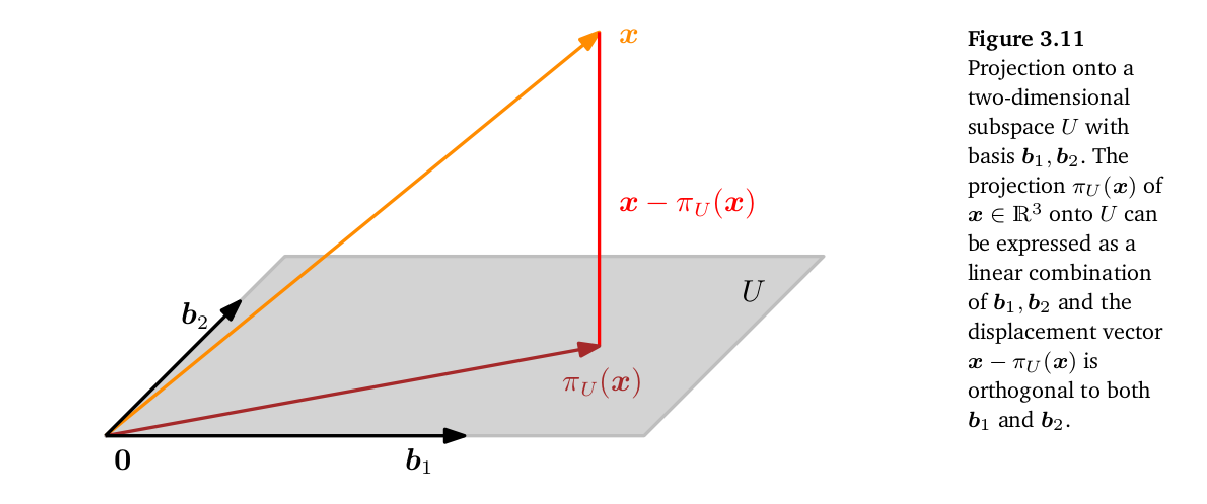
\includegraphics[width=0.95\textwidth,height=0.78\textheight,keepaspectratio]{figures/notes-md/N-20260305/N-20260305-fig-01-projection-onto-two-dimensional-subspace.png}
\caption{Projection onto a two-dimensional subspace: the residual \(x-\pi_U(x)\) is orthogonal to the basis directions of \(U\).}
\end{figure}

\section{Bridge to later ideas}

Projection is the geometric heart of least squares: the best approximation is characterized not by making the error small in every coordinate, but by making the error orthogonal to every allowed correction direction.



\paragraph{Expanded synthesis.}
For this chapter, the elementary material should be read as a study of what remains invariant when coordinates change. The earlier sections (`Projection onto a subspace`, `Projection matrix and least squares`, `Pseudoinverse`, `Higher viewpoint`) compute with arrays, bases, pivots, determinants, or eigenvectors; the deeper object is a linear map together with the spaces it acts on. A matrix is a representation of that map after bases have been chosen. This is why formulas such as
\[
  A' = P^{-1}AP,\qquad \widetilde A = T^{-1}AS
\]
are not cosmetic: they distinguish an intrinsic morphism from a coordinate description.

The structural hierarchy is as follows. Kernels record what a map forgets, images record what it reaches, cokernels record obstructions to solvability, and quotients record information after an equivalence has been imposed. Determinants act on the top exterior power and therefore measure oriented volume; traces are invariant under cyclic rearrangement and become characters in representation theory; adjoints depend on an inner product and lead to self-adjoint spectral theory.

A useful way to return to the computations is to ask, for every formula, which invariant it is measuring. Row reduction measures rank and kernel; diagonalization measures decomposition into invariant subspaces; Gram--Schmidt measures orthogonal projection; positive definiteness measures ellipsoid geometry; tensor notation measures how components transform. The elementary methods are therefore the finite-dimensional laboratory in which duality, quotienting, functoriality, and spectral decomposition can be seen clearly.


\section{Expanded derivation of the normal equations}

The formula for projection should not be memorized before the geometry is clear.  We want $B\lambda$ to be the closest vector in the column space of $B$ to $x$.  This means the error
\[
  e=x-B\lambda
\]
should be perpendicular to every vector in that column space.  Since the columns of $B$ span the space, this is equivalent to
\[
  B^T(x-B\lambda)=0.
\]
Hence
\[
  B^TB\lambda=B^Tx.
\]
If the columns of $B$ are independent, then $B^TB$ is positive definite and invertible.

\section{Four fundamental subspaces}

Projection is also a doorway to the four-subspace picture.  For a matrix $A$, the column space and left null space are orthogonal complements in the output space:
\[
  \mathbb R^m=\operatorname{Col}(A)\oplus \operatorname{Null}(A^T).
\]
Least squares solves $Ax\approx b$ by replacing $b$ with its projection onto $\operatorname{Col}(A)$.  The residual lies in $\operatorname{Null}(A^T)$.

\section{Pseudoinverse and minimum-norm solutions}

When $A$ is not full column rank, there may be many least-squares solutions.  The Moore--Penrose pseudoinverse selects the one with minimum norm.  Through SVD,
\[
  A=U\Sigma V^T,\qquad A^+=V\Sigma^+U^T.
\]
Small singular values are precisely the directions where inverse problems become unstable.

\notechapter{N-20260311}{Matrix Computation I: Norms, Operators, and Numerical Size}

\section{Why size matters}

Matrix computation starts from a simple question: how large can an error become after a linear operation acts on it?  A vector norm measures the size of data; a matrix norm measures the size of an operator.  In machine learning language, these are the quantities behind amplification, Lipschitz constants, gradient growth, and numerical stability.

A matrix is an operator
\[
  x\longmapsto Ax.
\]
To control it we need both
\[
  \text{vector size}\qquad\text{and}\qquad\text{operator size}.
\]

\section{Metrics and completeness}

A metric on a set \(X\) is a function \(d:X\times X\to[0,\infty)\) satisfying positivity, symmetry, and the triangle inequality.  It defines convergence.  A sequence is Cauchy if
\[
  \forall \varepsilon>0,\ \exists N,
  \quad m,n>N\Rightarrow d(x_m,x_n)<\varepsilon.
\]
A metric space is complete if every Cauchy sequence converges in it.  Completeness means that limiting procedures stay inside the space.

The discrete metric is a useful warning: not every metric expresses the geometry we want.  For numerical work, metrics induced by norms are the central examples.

\section{Normed vector spaces}

A norm satisfies
\[
  \|x\|=0\Leftrightarrow x=0,\qquad
  \|\alpha x\|=|\alpha|\|x\|,\qquad
  \|x+y\|\le \|x\|+\|y\|.
\]
It induces the metric
\[
  d(x,y)=\|x-y\|.
\]
A complete normed vector space is a Banach space.

In finite dimension, all norms are equivalent: for two norms \(\|\cdot\|_a,\|\cdot\|_b\), there exist constants \(c,C>0\) such that
\[
  c\|x\|_a\le \|x\|_b\le C\|x\|_a.
\]
Thus finite-dimensional convergence does not depend on the chosen norm, although numerical constants do.

\section{Standard vector norms}

For \(x=(x_1,\ldots,x_n)^T\),
\[
  \|x\|_1=\sum_i |x_i|,\qquad
  \|x\|_2=\left(\sum_i |x_i|^2\right)^{1/2},\qquad
  \|x\|_\infty=\max_i |x_i|.
\]
More generally,
\[
  \|x\|_p=\left(\sum_i |x_i|^p\right)^{1/p},\qquad 1\le p<\infty.
\]
As \(p\to\infty\),
\[
  \|x\|_p\to\|x\|_\infty.
\]
Holder's inequality gives
\[
  \sum_i |x_i y_i|\le \|x\|_p\|y\|_q,\qquad \frac1p+\frac1q=1,
\]
and Minkowski's inequality gives the triangle inequality for \(p\)-norms.

\section{Matrix norms}

A matrix norm satisfies the norm axioms and, for computation, should also be submultiplicative:
\[
  \|AB\|\le \|A\|\|B\|.
\]
This is what allows repeated operations to be bounded:
\[
  \|A^k\|\le \|A\|^k.
\]
Entrywise examples include
\[
  m_1(A)=\sum_{i,j}|a_{ij}|,\qquad
  \|A\|_F=\left(\sum_{i,j}|a_{ij}|^2\right)^{1/2}.
\]
The Frobenius norm also satisfies
\[
  \|A\|_F^2=\operatorname{tr}(A^H A).
\]

\section{Unitary invariance}

A matrix \(U\) is unitary if \(U^HU=I\).  It preserves Euclidean length:
\[
  \|Ux\|_2=\|x\|_2.
\]
The Frobenius norm is unitarily invariant:
\[
  \|UAV\|_F=\|A\|_F
\]
for unitary \(U,V\).  This follows from cyclic invariance of trace:
\[
  \|UAV\|_F^2=\operatorname{tr}(V^HA^HAV)=\operatorname{tr}(A^HA).
\]
Unitary transformations are changes of orthonormal coordinates, not changes of size.

\section{Induced norms}

Given vector norms on domain and codomain, the induced matrix norm is
\[
  \|A\|=\max_{x\ne0}\frac{\|Ax\|}{\|x\|}
  =\max_{\|x\|=1}\|Ax\|.
\]
It is the maximal amplification factor of \(A\).  The standard formulas are
\[
  \|A\|_1=\max_j\sum_i |a_{ij}|,\qquad
  \|A\|_\infty=\max_i\sum_j |a_{ij}|,
\]
and
\[
  \|A\|_2=\sigma_{\max}(A)=\sqrt{\lambda_{\max}(A^H A)}.
\]
The \(2\)-norm is the spectral norm.

\section{Normal matrices}

A matrix is Hermitian if \(A^H=A\), skew-Hermitian if \(A^H=-A\), and normal if
\[
  A^HA=AA^H.
\]
Normal matrices are unitarily diagonalizable.  If
\[
  A=U\Lambda U^H,
\]
then
\[
  \|A\|_2=\max_i |\lambda_i|.
\]
For nonnormal matrices, eigenvalues may seriously underestimate transient amplification.

\section{Compatibility}

A vector norm and a matrix norm are compatible if
\[
  \|Ax\|\le \|A\|\|x\|.
\]
Every induced matrix norm is compatible with the vector norm that induces it.  Compatibility is the bridge from operator size to error propagation:
\[
  \|A(x+\delta x)-Ax\|\le \|A\|\|\delta x\|.
\]

\section{Worked constrained maxima}

Let
\[
  A=\begin{bmatrix}1&1&0\\1&1&0\\0&0&2\end{bmatrix}.
\]
Then \(A\) is Hermitian with eigenvalues \(2,2,0\).  Hence
\[
  \|A\|_2=2.
\]
The column sums are all \(2\), so \(\|A\|_1=2\).  Therefore
\[
  \max_{\|x\|_1=4}\|Ax\|_1=8.
\]
If \(U\) is unitary and \(\|Ux\|_2=3\), then \(\|x\|_2=3\), hence
\[
  \max_{\|Ux\|_2=3}\|Ax\|_2=6.
\]
The method is: translate the constraint into a norm ball and apply the induced norm.

\section{ML-facing interpretation}

A linear layer has Lipschitz constant at most \(\|W\|_2\) in Euclidean norm.  A stack obeys
\[
  \|W_L\cdots W_1\|_2\le \prod_{\ell=1}^L\|W_\ell\|_2.
\]
This inequality is crude but important: moderate layerwise amplification can accumulate over depth.  Spectral normalization, orthogonal initialization, residual scaling, and weight decay are all connected to the same numerical question: how large can a perturbation become?

\section{What each norm is measuring}

\[
\begin{array}{c|c|c}
\text{object} & \text{what it measures} & \text{typical use}\\
\hline
\text{metric} & \text{distance between two points} & \text{convergence and continuity}\\
\text{vector norm} & \text{size of one vector} & \text{error magnitude}\\
\text{induced matrix norm} & \max_{x\ne0}\|Ax\|/\|x\| & \text{worst-case amplification}\\
\text{Frobenius norm} & \sqrt{\sum_{ij}|a_{ij}|^2} & \text{entrywise energy}\\
\text{spectral norm} & \sigma_{\max}(A) & \text{Euclidean Lipschitz bound}
\end{array}
\]
The worked constrained-maximum examples explain the difference between Frobenius and spectral size.  Frobenius norm counts all entries at once, while the spectral norm asks for the single input direction that is stretched the most.  In the linear-layer interpretation, \(\|W\|_2\) is therefore the relevant bound for adversarial or perturbation amplification, whereas \(\|W\|_F\) is a global weight-size penalty.  The inequality
\[
  \|W_L\cdots W_1\|_2\le \prod_{\ell=1}^L\|W_\ell\|_2
\]
should be read as a warning about composition: even if each layer is controlled separately, the product controls how errors can accumulate through the whole map.

\notechapter{N-20260312}{Spectral Radius, Matrix Series, and Numerical Conditioning}


\section{Spectral radius}

For $A\in\mathbb C^{n\times n}$ with eigenvalues $\lambda_1,\ldots,\lambda_n$, the spectral radius is
\[
  \rho(A)=\max_j |\lambda_j|.
\]
For any operator norm,
\[
  \rho(A)\le \|A\|.
\]
Indeed, if $Ax=\lambda x$ and $x\ne0$, then $|\lambda|\|x\|=\|Ax\|\le\|A\|\|x\|$.

\section{Powers and convergence}

The long-term behavior of $A^k$ is controlled by $\rho(A)$.  In finite dimension,
\[
  A^k\to0\quad\Longleftrightarrow\quad \rho(A)<1.
\]
The Jordan form explains the borderline cases: a block with eigenvalue $|\lambda|<1$ decays even with polynomial factors, while $|\lambda|\ge1$ prevents decay.

\section{Matrix geometric series}

If $\rho(A)<1$, then
\[
  \sum_{k=0}^\infty A^k=(I-A)^{-1}.
\]
This is the matrix version of the scalar geometric series.  The condition is not merely $\|A\|<1$ for a particular norm; $\rho(A)<1$ is the intrinsic condition, although a suitable norm can often be chosen with $\|A\|<1$.

\section{Condition number}

For an invertible matrix $A$, the condition number in a norm is
\[
  \kappa(A)=\|A\|\|A^{-1}\|.
\]
It measures how much relative error can be amplified when solving $Ax=b$.  In the Euclidean norm,
\[
  \kappa_2(A)=\frac{\sigma_{\max}(A)}{\sigma_{\min}(A)}.
\]
A large condition number means the problem is intrinsically sensitive, not just that an algorithm is poorly written.

\section{Expanded synthesis and advanced context}

Spectral radius describes asymptotic dynamics, the matrix geometric series describes stable feedback, and condition number describes sensitivity to perturbation.  These are the linear-algebraic roots of many stability questions in numerical analysis and machine learning.



\paragraph{Expanded synthesis.}
For this chapter, the elementary material should be read as a study of what remains invariant when coordinates change. The earlier sections (`Spectral radius`, `Powers and convergence`, `Matrix geometric series`, `Condition number`, `Higher viewpoint`) compute with arrays, bases, pivots, determinants, or eigenvectors; the deeper object is a linear map together with the spaces it acts on. A matrix is a representation of that map after bases have been chosen. This is why formulas such as
\[
  A' = P^{-1}AP,\qquad \widetilde A = T^{-1}AS
\]
are not cosmetic: they distinguish an intrinsic morphism from a coordinate description.

The structural hierarchy is as follows. Kernels record what a map forgets, images record what it reaches, cokernels record obstructions to solvability, and quotients record information after an equivalence has been imposed. Determinants act on the top exterior power and therefore measure oriented volume; traces are invariant under cyclic rearrangement and become characters in representation theory; adjoints depend on an inner product and lead to self-adjoint spectral theory.

A useful way to return to the computations is to ask, for every formula, which invariant it is measuring. Row reduction measures rank and kernel; diagonalization measures decomposition into invariant subspaces; Gram--Schmidt measures orthogonal projection; positive definiteness measures ellipsoid geometry; tensor notation measures how components transform. The elementary methods are therefore the finite-dimensional laboratory in which duality, quotienting, functoriality, and spectral decomposition can be seen clearly.


\section{Expanded spectral-radius calculus}

The inequality $\rho(A)\le\|A\|$ is only the beginning.  Gelfand's formula says
\[
  \rho(A)=\lim_{k\to\infty}\|A^k\|^{1/k}
\]
for any matrix norm.  Thus spectral radius is the intrinsic exponential growth rate of powers of $A$.

This explains why $\rho(A)<1$ is the exact condition for $A^k\to0$.  If $A$ has a Jordan block $J=\lambda I+N$, then
\[
  J^k=\sum_{j=0}^{m-1}\binom{k}{j}\lambda^{k-j}N^j.
\]
The polynomial factor cannot defeat exponential decay when $|\lambda|<1$, but it matters on the boundary $|\lambda|=1$.

\section{Conditioning as geometry of inverse maps}

Solving $Ax=b$ applies $A^{-1}$ to $b$.  If $A$ sends some unit vector to a very short vector, then $A^{-1}$ must stretch that direction enormously.  In singular-value language,
\[
  \kappa_2(A)=\frac{\sigma_{\max}}{\sigma_{\min}}.
\]
A large condition number means small errors in $b$ may create large errors in $x$.

\notechapter{N-20260318}{Matrix Computation III: Canonical Forms, Localization, and Iteration}

\section{Why canonical forms matter}

Canonical forms explain what a matrix cannot hide under a change of basis.  For computation they answer: how do powers behave, where can eigenvalues be, and which direction dominates an iteration?

\section{Polynomial matrices}

A \(\lambda\)-matrix is a matrix whose entries lie in \(\mathbb C[\lambda]\).  Its rank is the largest order of a minor that is not the zero polynomial.  A square \(\lambda\)-matrix is nonsingular if its determinant is not the zero polynomial.

The elementary operations are row or column exchange, multiplication of a row or column by a nonzero constant, and adding \(\varphi(\lambda)\) times one row or column to another.

\section{Smith normal form}

Every rank \(r\) polynomial matrix is equivalent to
\[
  \operatorname{diag}(d_1(\lambda),\ldots,d_r(\lambda),0,\ldots,0),
\]
where each \(d_i\) is monic and
\[
  d_1\mid d_2\mid\cdots\mid d_r.
\]
This is the Smith normal form.

Let \(D_k(\lambda)\) be the monic greatest common divisor of all nonzero \(k\)-minors.  The invariant factors are
\[
  d_1=D_1,\qquad d_k=\frac{D_k}{D_{k-1}}.
\]
Factoring the nonconstant invariant factors gives elementary divisors.

\section{Jordan data from elementary divisors}

For \(A\in\mathbb C^{n\times n}\), apply Smith form to
\[
  \lambda I-A.
\]
An elementary divisor
\[
  (\lambda-\lambda_0)^s
\]
corresponds to a Jordan block of size \(s\) for eigenvalue \(\lambda_0\).

Thus Smith form is an algebraic route to Jordan structure.

\section{Jordan chains}

A Jordan block is
\[
  J_s(\lambda)=
  \begin{bmatrix}
  \lambda&1&&0\\
  &\lambda&\ddots&\\
  &&\ddots&1\\
  0&&&\lambda
  \end{bmatrix}.
\]
If \(A=PJP^{-1}\), the columns in one Jordan chain satisfy
\[
  Ap_1=\lambda p_1,\qquad
  Ap_i=\lambda p_i+p_{i-1}.
\]
The later vectors are generalized eigenvectors.

\section{Computing powers}

If \(J=\lambda I+N\) with \(N^s=0\), then
\[
  J^k=\sum_{j=0}^{s-1}\binom{k}{j}\lambda^{k-j}N^j.
\]
For \(A=PJP^{-1}\),
\[
  A^k=PJ^kP^{-1}.
\]
Jordan form explains polynomial factors in matrix powers.

\section{Gershgorin discs}

For \(A=(a_{ij})\), define
\[
  R_i=\sum_{j\ne i}|a_{ij}|.
\]
Every eigenvalue lies in
\[
  \bigcup_i \{z\in\mathbb C: |z-a_{ii}|\le R_i\}.
\]
Proof: choose \(i\) with \(|x_i|=\max_j|x_j|\) for an eigenvector \(x\).  From \(Ax=\lambda x\),
\[
  (\lambda-a_{ii})x_i=\sum_{j\ne i}a_{ij}x_j,
\]
so \(|\lambda-a_{ii}|\le R_i\).

\section{Gershgorin figure}

\begin{figure}[H]
\centering
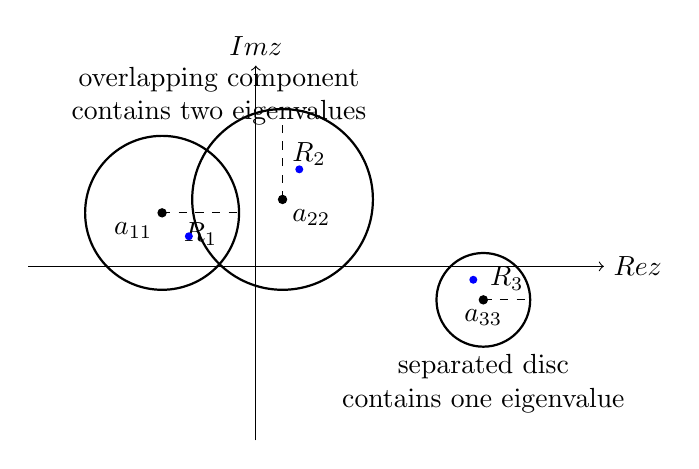
\begin{tikzpicture}[scale=0.85]
  \draw[->] (-3.4,0) -- (5.2,0) node[right] {$\operatorname{Re}z$};
  \draw[->] (0,-2.6) -- (0,3.0) node[above] {$\operatorname{Im}z$};
  \coordinate (c1) at (-1.4,0.8);
  \coordinate (c2) at (0.4,1.0);
  \coordinate (c3) at (3.4,-0.5);
  \draw[thick] (c1) circle (1.15);
  \draw[thick] (c2) circle (1.35);
  \draw[thick] (c3) circle (0.7);
  \fill (c1) circle (2pt) node[below left] {$a_{11}$};
  \fill (c2) circle (2pt) node[below right] {$a_{22}$};
  \fill (c3) circle (2pt) node[below] {$a_{33}$};
  \draw[dashed] (c1) -- ++(1.15,0) node[midway,below] {$R_1$};
  \draw[dashed] (c2) -- ++(0,1.35) node[midway,right] {$R_2$};
  \draw[dashed] (c3) -- ++(0.7,0) node[midway,above] {$R_3$};
  \node[align=center] at (-0.55,2.55) {overlapping component\\contains two eigenvalues};
  \node[align=center] at (3.4,-1.75) {separated disc\\contains one eigenvalue};
  \fill[blue] (-1.0,0.45) circle (1.7pt);
  \fill[blue] (0.65,1.45) circle (1.7pt);
  \fill[blue] (3.25,-0.2) circle (1.7pt);
\end{tikzpicture}
\caption{Gershgorin discs localize eigenvalues.  A separated component containing one disc contains exactly one eigenvalue.}
\end{figure}

\section{Separated components and scaling}

If a connected component of the union of Gershgorin discs consists of exactly \(m\) discs and is separated from the others, then it contains exactly \(m\) eigenvalues.

Column Gershgorin discs can be obtained by applying the theorem to \(A^T\).  Diagonal similarity
\[
  D^{-1}AD
\]
does not change eigenvalues but changes radii, since
\[
  (D^{-1}AD)_{ij}=d_i^{-1}a_{ij}d_j.
\]
This is a practical way to improve localization.

\section{Power iteration}

If
\[
  |\lambda_1|>|\lambda_2|\ge\cdots,
\]
and the initial vector has a nonzero component in the dominant eigenvector direction, then
\[
  u_{k+1}=\frac{Au_k}{\|Au_k\|}
\]
converges toward the dominant eigenvector direction.  The convergence rate is governed by
\[
  \left|\frac{\lambda_2}{\lambda_1}\right|.
\]

\section{Inverse and shifted inverse iteration}

Inverse iteration applies power iteration to \(A^{-1}\), so it finds eigenvalues of small modulus.  Shifted inverse iteration applies inverse iteration to
\[
  A-pI.
\]
Eigenvalues of \((A-pI)^{-1}\) are
\[
  \frac1{\lambda_j-p}.
\]
Thus the eigenvalue closest to \(p\) becomes dominant.

\section{Numerical traps}

Shifted inverse iteration requires solving systems with \(A-pI\), which may be nearly singular.  This is why the method can be powerful and unstable at the same time.  Pivoting and residual checks are essential.

Gershgorin discs are cheap localization, not exact computation.  Overlap does not mean eigenvalues are evenly spread through the overlap.

\section{ML-facing interpretation}

Power iteration appears in PageRank, spectral normalization, graph propagation, and monitoring dominant eigenvalue behavior.  State-space and recurrent models depend on polynomial and spectral structure: the minimal polynomial, Jordan blocks, and spectral radius all describe memory and long-run dynamics.

\section{Checklist}

\[
\begin{array}{c|c}
\text{Smith form} & \text{invariant factors}\\
\text{Jordan form} & \text{eigenvalue chains}\\
\text{Gershgorin} & \text{cheap eigenvalue regions}\\
\text{power iteration} & \text{dominant eigenvalue}\\
\text{shifted inverse iteration} & \text{eigenvalue near target}
\end{array}
\]

\notechapter{N-20260602}{Matrix Decompositions: LU, Cholesky, Full Rank, and SVD}

\section{Why decompositions are algorithms}
A decomposition rewrites a matrix into factors that are easier to compute with.  LU reduces a system to triangular solves; Cholesky uses positive definiteness; full-rank decomposition exposes rank; SVD exposes singular directions.

\section{Doolittle LU}
If \(A\in\mathbb C^{n\times n}\) can be written as
\[
  A=LU,
\]
where \(L\) is unit lower triangular and \(U\) is upper triangular, this is the Doolittle or LU decomposition.

\section{Existence and uniqueness}
If the first \(n-1\) leading principal minors of \(A\) are nonzero, then \(A=LU\) exists.  If \(A\) is nonsingular, the decomposition is unique.  The condition says that Gaussian elimination without row exchange never meets a zero pivot.

\section{Elimination matrices}
At step \(k\), an elimination matrix \(L_k\) zeros entries below the pivot.  After all steps,
\[
  L_{n-1}\cdots L_1A=U,\qquad
  A=L_1^{-1}\cdots L_{n-1}^{-1}U.
\]
The product of the inverses is the lower triangular factor.

\section{Doolittle formulas}
Comparing \(A=LU\) gives
\[
  u_{kj}=a_{kj}-\sum_{t=1}^{k-1}l_{kt}u_{tj},\qquad j\ge k,
\]
\[
  l_{ik}=\frac{1}{u_{kk}}\left(a_{ik}-\sum_{t=1}^{k-1}l_{it}u_{tk}\right),\qquad i>k.
\]
The pivot \(u_{kk}\) must be nonzero.

\section{Pivoting}
If a pivot is zero or small, row exchange is needed.  With partial pivoting,
\[
  PA=LU,
\]
where \(P\) is a permutation matrix.  Pivoting controls large multipliers and improves numerical stability.

\section{Storage of LU}
The upper triangle stores \(U\); the strictly lower triangle stores the multipliers \(l_{ij}\).  The diagonal of \(L\) is omitted because it is all ones.

\section{Cholesky decomposition}
If \(A\) is Hermitian positive definite, there is a unique lower triangular \(L\) with positive diagonal such that
\[
  A=LL^H.
\]
Solving \(Ax=b\) becomes
\[
  Ly=b,\qquad L^Hx=y.
\]
Cholesky costs about \(\frac13n^3+O(n^2)\), roughly half of LU.

\section{Cholesky example}
For
\[
  A=\begin{bmatrix}4&2\\2&5\end{bmatrix},
\]
we obtain
\[
  L=\begin{bmatrix}2&0\\1&2\end{bmatrix},\qquad A=LL^T.
\]

\section{Full-rank decomposition}
If \(\operatorname{rank}A=r>0\), a full-rank decomposition is
\[
  A=FG,\qquad F\in\mathbb C^{m\times r},\quad G\in\mathbb C^{r\times n},
\]
with both factors rank \(r\).  It always exists and is not unique.

\section{Hermite standard form}
Row operations reduce \(A\) to a Hermite-style form \(H\).  If pivot columns are \(j_1,\ldots,j_r\), choose \(F\) as the corresponding columns of \(A\), and \(G\) as the nonzero rows of \(H\).  Then \(A=FG\).

\section{Singular values}
The singular values of \(A\) are
\[
  \sigma_i=\sqrt{\lambda_i(A^HA)}.
\]
Unitary equivalence preserves singular values.

\section{Singular value decomposition}
If \(\operatorname{rank}A=r\), then
\[
  A=U\begin{bmatrix}\Sigma&0\\0&0\end{bmatrix}V^H,\qquad
  \Sigma=\operatorname{diag}(\sigma_1,\ldots,\sigma_r).
\]
SVD says that \(A\) rotates, stretches along orthogonal axes, and rotates again.

\section{SVD geometry}
\begin{figure}[H]
\centering
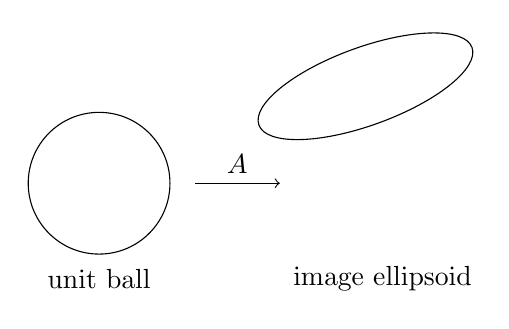
\begin{tikzpicture}[scale=0.9]
  \draw (0,0) circle (1);
  \node at (0,-1.35) {unit ball};
  \draw[->] (1.35,0) -- (2.55,0) node[midway,above] {$A$};
  \draw[rotate=20] (4,0) ellipse (1.6 and 0.55);
  \node at (4,-1.35) {image ellipsoid};
\end{tikzpicture}
\caption{SVD describes the image of the unit ball as an ellipsoid.}
\end{figure}

\section{Which decomposition matches the matrix}

\begin{center}
\small
\begin{tabularx}{\textwidth}{@{}lYY@{}}
\toprule
Decomposition & Hypothesis or signal & What it gives\\
\midrule
\(LU\) & square system without severe pivot trouble & triangular solves\\
\(PA=LU\) & row exchanges needed & stable Gaussian elimination\\
\(A=LL^H\) & Hermitian positive definite & fast symmetric solve\\
\(A=FG\) & \(\operatorname{rank}A=r\) & factorization through an \(r\)-dimensional space\\
\(A=U\Sigma V^H\) & arbitrary rectangular matrix & singular directions and rank profile\\
\bottomrule
\end{tabularx}
\end{center}
The choice should be driven by structure rather than by habit.  Cholesky is inappropriate without positive definiteness; ordinary LU may need pivoting when a small or zero pivot appears; a full-rank decomposition records the actual dimension through which the linear map factors.  The SVD is the most geometric option: it says that the unit ball is rotated, stretched by the singular values, and rotated again.  This is why the nonzero singular values detect rank and why small singular values signal directions in which solving or inversion will be unstable.

\notechapter{N-20260603}{Generalized Inverses, Projections, and Least-Squares Geometry}

\section{Why ordinary inverse is not enough}
For \(A\in\mathbb C^{m\times n}\), the system \(Ax=b\) may be overdetermined, underdetermined, singular, or rank deficient.  The Moore-Penrose inverse \(A^+\) gives a unified optimal answer.

\section{Four regimes}
\[
\begin{array}{c|c|c|c}
I&m=n&r=n&\text{ordinary inverse}\\
II&m>n&r=n&\text{least squares}\\
III&m<n&r=m&\text{minimum norm}\\
IV&\text{any}&r<\min(m,n)&\text{rank deficient}
\end{array}
\]

\section{Penrose equations}
The Moore-Penrose inverse is the unique \(X\) satisfying
\[
  AXA=A,\quad XAX=X,\quad (AX)^H=AX,\quad (XA)^H=XA.
\]
It is denoted \(A^+\).

\section{Fifteen generalized inverses}
Choosing any nonempty subset of the four Penrose equations gives one of \(15\) generalized-inverse classes.  Only the Moore-Penrose inverse is unique for every matrix.

\section{Projection transformations}
If \(\mathbb C^n=L\oplus M\), the projection onto \(L\) along \(M\) maps \(x=y+z\) to \(y\), where \(y\in L,z\in M\).

\section{Idempotence and orthogonality}
A matrix is a projection iff
\[
  P^2=P.
\]
It is an orthogonal projection iff
\[
  P^2=P,\qquad P^H=P.
\]

\section{Column and row-space projections}
\(AA^+\) is the orthogonal projection onto \(R(A)\).  \(A^+A\) is the orthogonal projection onto \(R(A^H)\).

\begin{figure}[H]
\centering
\begin{tikzpicture}[scale=0.95]
  \draw[->] (-2.8,0) -- (2.8,0) node[right] {$R(A)$};
  \draw[->] (0,-1.7) -- (0,2.1) node[above] {$R(A)^\perp$};
  \draw[->,thick] (0,0) -- (1.8,1.2) node[right] {$b$};
  \draw[->,thick] (0,0) -- (1.8,0) node[below] {$AA^+b$};
  \draw[dashed] (1.8,0) -- (1.8,1.2);
\end{tikzpicture}
\caption{The vector \(AA^+b\) is the orthogonal projection of \(b\) onto the column space.}
\end{figure}

\section{SVD computation}
If
\[
  A=U\begin{bmatrix}\Sigma&0\\0&0\end{bmatrix}V^H,
\]
then
\[
  A^+=V\begin{bmatrix}\Sigma^{-1}&0\\0&0\end{bmatrix}U^H.
\]
Only nonzero singular values are inverted.

\section{Full-rank computation}
If \(A=FG\) is a full-rank decomposition, then
\[
  A^+=G^H(GG^H)^{-1}(F^HF)^{-1}F^H.
\]

\section{Greville recursion}
Greville's method updates \(A_k^+\) when a new column is appended.  It is useful for column-by-column or online data, although numerical stability still requires care.

\section{Iterative approximations}
Iterative methods for \(A^+\) often require a step size satisfying a condition such as
\[
  0<\alpha<\frac{2}{\sigma_{\max}^2}.
\]
Convergence is again a spectral-radius issue.

\section{Solvability}
The system \(Ax=b\) is solvable iff
\[
  AA^+b=b.
\]
If it is solvable, the general solution is
\[
  x=A^+b+(I-A^+A)y.
\]

\section{Least squares and minimum norm}
For every \(b\), \(A^+b\) is the least-squares solution minimizing \(\|Ax-b\|_2\).  Among all minimizers, it has minimum \(2\)-norm.

\section{Identities}
\[
  (A^+)^+=A,\qquad (A^H)^+=(A^+)^H,\qquad \operatorname{rank}A^+=\operatorname{rank}A.
\]
In general, \((AB)^+\ne B^+A^+\) without additional assumptions.

\section{Checklist}
\[
\begin{array}{c|c}
A^+ & \text{Moore-Penrose inverse}\\
AA^+ & \text{projection onto }R(A)\\
A^+A & \text{projection onto }R(A^H)\\
AA^+b=b & \text{solvability}\\
A^+b & \text{least-squares minimum-norm solution}
\end{array}
\]

\notechapter{N-20260604}{Solving Linear Systems: Direct, Iterative, and Optimization Methods}

\section{The computational problem}
Solving \(Ax=b\) can be done by direct methods, iterative methods, or optimization methods.  Structure decides which method is appropriate.

\section{Triangular solves}
For lower triangular \(L\), forward substitution gives
\[
  y_i=\frac{1}{l_{ii}}\left(b_i-\sum_{j<i}l_{ij}y_j\right).
\]
For upper triangular \(U\), backward substitution gives
\[
  x_i=\frac{1}{u_{ii}}\left(y_i-\sum_{j>i}u_{ij}x_j\right).
\]

\section{Gauss elimination}
At step \(k\), with pivot \(a_{kk}^{(k)}\ne0\), set
\[
  l_{ik}=-\frac{a_{ik}^{(k)}}{a_{kk}^{(k)}}.
\]
Then update
\[
  a_{ij}^{(k+1)}=a_{ij}^{(k)}+l_{ik}a_{kj}^{(k)},\qquad
  b_i^{(k+1)}=b_i^{(k)}+l_{ik}b_k^{(k)}.
\]
After \(n-1\) steps one solves an upper triangular system.

\section{Pivoting}
Small pivots amplify rounding error.  Partial pivoting swaps the largest available entry in the current column into the pivot position.  Algebraically,
\[
  PA=LU.
\]

\section{LU solution}
If \(A=LU\), solve
\[
  Ly=b,\qquad Ux=y.
\]
If \(PA=LU\), solve
\[
  Ly=Pb,\qquad Ux=y.
\]

\section{Cholesky and LDL}
For Hermitian positive definite \(A\), use
\[
  A=LL^H.
\]
The improved square-root method uses
\[
  A=LDL^H,
\]
where \(L\) is unit lower triangular and \(D\) is positive diagonal.  Then solve \(Ly=b\), \(Dz=y\), \(L^Hx=z\).

\section{Tridiagonal chasing}
A tridiagonal system can be solved in linear time by a specialized LU factorization.  The forward sweep computes modified coefficients; the backward sweep recovers \(x_n,x_{n-1},\ldots,x_1\).

\section{Stationary iteration}
Rewrite \(Ax=b\) as
\[
  x=Bx+f,\qquad x^{(k+1)}=Bx^{(k)}+f.
\]
The error satisfies
\[
  e^{(k+1)}=Be^{(k)}.
\]
Thus convergence for every starting vector is equivalent to
\[
  \rho(B)<1.
\]

\section{Jacobi iteration}
With \(A=D+L+U\), Jacobi uses
\[
  x^{(k+1)}=-D^{-1}(L+U)x^{(k)}+D^{-1}b.
\]
Componentwise,
\[
  x_i^{(k+1)}=\frac{1}{a_{ii}}\left(b_i-\sum_{j\ne i}a_{ij}x_j^{(k)}\right).
\]

\section{Gauss-Seidel iteration}
Gauss-Seidel uses the newest available values:
\[
  x^{(k+1)}=-(D+L)^{-1}Ux^{(k)}+(D+L)^{-1}b.
\]
Componentwise,
\[
  x_i^{(k+1)}=\frac{1}{a_{ii}}\left(b_i-\sum_{j<i}a_{ij}x_j^{(k+1)}-\sum_{j>i}a_{ij}x_j^{(k)}\right).
\]

\section{Diagonal dominance}
If
\[
  |a_{ii}|>\sum_{j\ne i}|a_{ij}|
\]
for every row, then Jacobi and Gauss-Seidel converge.  Irreducible weak diagonal dominance gives another standard sufficient condition.

\section{SOR iteration}
SOR introduces a relaxation parameter \(\alpha\):
\[
  B_\alpha=(D+\alpha L)^{-1}((1-\alpha)D-\alpha U).
\]
For real symmetric positive definite \(A\), SOR converges iff
\[
  0<\alpha<2.
\]

\section{Optimization viewpoint}
If \(A\) is Hermitian positive definite, solving \(Ax=b\) is equivalent to minimizing
\[
  \phi(x)=\frac12 x^H A x-\operatorname{Re}(b^H x).
\]
Its gradient is \(Ax-b\).

\section{Steepest descent}
Let \(r_k=Ax_k-b\).  Steepest descent uses
\[
  x_{k+1}=x_k-\alpha_k r_k,\qquad
  \alpha_k=\frac{(r_k,r_k)}{(Ar_k,r_k)}.
\]
It decreases the quadratic energy, but may be slow when \(\kappa(A)\) is large.

\section{Method map}
\begin{figure}[H]
\centering
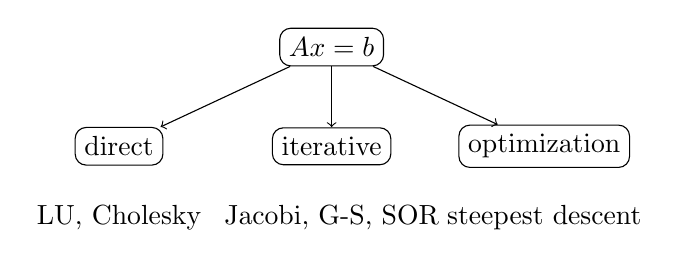
\begin{tikzpicture}[scale=0.9]
  \node[draw,rounded corners] (A) at (0,0) {$Ax=b$};
  \node[draw,rounded corners] (D) at (-3,-1.4) {direct};
  \node[draw,rounded corners] (I) at (0,-1.4) {iterative};
  \node[draw,rounded corners] (O) at (3,-1.4) {optimization};
  \draw[->] (A) -- (D); \draw[->] (A) -- (I); \draw[->] (A) -- (O);
  \node at (-3,-2.4) {LU, Cholesky};
  \node at (0,-2.4) {Jacobi, G-S, SOR};
  \node at (3,-2.4) {steepest descent};
\end{tikzpicture}
\caption{Linear systems can be solved by factorization, iteration, or minimization.}
\end{figure}

\section{Checklist}
\[
\begin{array}{c|c}
\text{Gauss} & \text{triangularize}\\
\text{pivoting} & \text{avoid small pivots}\\
\text{Cholesky} & \text{positive definite}\\
\text{chasing} & \text{tridiagonal}\\
\text{iteration} & \rho(B)<1\\
\text{SOR} & 0<\alpha<2\text{ for SPD}\\
\text{steepest descent} & \text{quadratic minimization}
\end{array}
\]



\part{Calculus and Inequalities}
\label{vol:08-calculus-and-inequalities}
\begingroup
\small
\sloppy
\parttoc
\endgroup

% This file is generated during volume reorganization.
% Volume: Calculus and Inequalities

\notechapter{N-20220315}{Quadratic Parameters, Tangency, and Constrained Extrema}

\section{A scattered algebraic note}

The original page is titled ``some scattered things.''  The common theme is that elementary-looking algebraic problems often hide a parameter, a tangency condition, or an extremum under constraint.  I rewrite the problems in a more systematic form.

\section{A quadratic with parameters}

Let
\[
  f(x)=ax^2+bx+c,\qquad a<b<c,
\]
and suppose the graph passes through \(A=(1,0)\) and \(B=(m,-a)\).  The condition \(f(1)=0\) gives
\[
  a+b+c=0.
\]
The condition \(f(m)=-a\) is equivalent to saying that \(f(x)+a\) has \(x=m\) as a root:
\[
  am^2+bm+c+a=0.
\]
Using \(c=-a-b\), this becomes
\[
  am^2+bm-b=0,\qquad am^2=-b(m-1).
\]
The axis of symmetry is
\[
  x_0=-\frac{b}{2a}.
\]
Thus the parameter \(m\) and the axis \(x_0\) are tied by
\[
  x_0=\frac{m^2}{2m-2}.
\]
Equivalently,
\[
  m^2=(2m-2)x_0,\qquad m^2-2x_0m+2x_0=0.
\]
Solving for \(m\) gives
\[
  m=x_0\pm\sqrt{x_0^2-2x_0}.
\]
The original calculation uses this relation to examine endpoints and stationary points of \(m\) as a function of \(x_0\).  The conclusion is that the extremal parameter occurs at
\[
  x_0=0\quad\text{or}\quad x_0=-\frac12,
\]
and the relevant value is
\[
  m=\frac{\sqrt5-1}{2}.
\]
This is a small example of a recurring trick: convert the algebraic parameter into a geometric parameter, usually the axis, vertex, or tangency point.

\section{A parabola and a hyperbola}

The second problem considers the parabola
\[
  y=x^2-2ax+a^2-4=(x-a)^2-4
\]
and the rectangular hyperbola
\[
  y=\frac{k}{x},\qquad k>0,
\]
in the first quadrant.  The intersection equation is
\[
  x^2-2ax+a^2-4=\frac{k}{x},\qquad x>0,
\]
or
\[
  x^3-2ax^2+(a^2-4)x-k=0.
\]
Questions about ``only one intersection'' are therefore tangency or root-counting questions for this cubic, but the geometry is usually cleaner: one restricts to the right side of the parabola, because the branch \(k/x\) lies in the first quadrant.

\begin{remark}
The hidden principle is that a graph-intersection problem may become either a polynomial root-counting problem or a tangency problem.  The latter is often more geometric and less computational.
\end{remark}

\section{A constrained extremum}

The third problem asks for extrema of
\[
  x+y
\]
under the constraint
\[
  x^2+y^3=2.
\]
Using Lagrange multipliers for
\[
  F(x,y,\lambda)=x+y+\lambda(x^2+y^3-2),
\]
we get
\[
  1+2\lambda x=0,\qquad
  1+3\lambda y^2=0,\qquad
  x^2+y^3=2.
\]
Eliminating \(\lambda\) gives
\[
  2x=3y^2.
\]
Hence
\[
  x=\frac32y^2.
\]
Substitution into the constraint gives
\[
  \frac94y^4+y^3=2,
\]
so the stationary points come from the quartic
\[
  9y^4+4y^3-8=0.
\]
The numerical plot in the original note marks approximately
\[
  A=(1.15195,2.02829),\qquad B=(1.82947,0.72509),
\]
for the function
\[
  h(x)=x+(2-x^2)^{1/3}.
\]
These are the local maximum and local minimum along the real branch.

\begin{figure}[H]
\centering
\begin{tikzpicture}[scale=1.2,>=Stealth,every node/.style={fill=white,inner sep=1.2pt}]
  \draw[->] (-1.5,0)--(4.3,0) node[right] {$x$};
  \draw[->] (0,-1.25)--(0,3.2) node[above] {$y$};
  \draw[smooth,thick] plot coordinates {(-1.2,-0.45) (-0.5,0.55) (0,1.26) (0.6,1.78) (1.15,2.03) (1.45,1.55) (1.83,0.73) (2.5,0.95) (4.0,1.65)};
  \fill (1.15,2.03) circle (0.04);
  \node[above left=2pt] at (1.15,2.03) {$A\approx(1.15,2.03)$};
  \fill (1.83,0.73) circle (0.04);
  \node[below right=2pt] at (1.83,0.73) {$B\approx(1.83,0.73)$};
  \node[below] at (2.25,-0.55) {$y=x+(2-x^2)^{1/3}$};
\end{tikzpicture}
\caption{Reconstruction of the graph used for the constrained extremum problem.}
\end{figure}


\section{Tangency as a double-root condition}

A parameter problem involving a quadratic often asks when a line is tangent to a parabola or when an equation has exactly one solution.  Algebraically, this is a discriminant condition:
\[
  \Delta=b^2-4ac=0.
\]
Geometrically, the line touches the parabola at one point.  The same idea appears in constrained extrema: a level curve just touches a constraint curve at an optimum.

\section{Completing the square}

For a quadratic
\[
  ax^2+bx+c,\qquad a\ne0,
\]
completing the square gives
\[
  a\left(x+\frac b{2a}\right)^2+c-\frac{b^2}{4a}.
\]
This form reveals the vertex, minimum or maximum value, and symmetry axis.  It is usually more informative than the expanded form.

\section{Expanded synthesis and advanced context}

The three examples are connected by the same idea: reduce a complicated statement to a structural condition.  The axis of a quadratic, the tangency of two graphs, and the Lagrange multiplier equations are all ways of saying that an extremum occurs when a first-order freedom disappears.


\paragraph{Expanded synthesis.}
For this chapter, the elementary material should be read as a study of what remains invariant when coordinates change. The earlier sections (`A scattered algebraic note`, `A quadratic with parameters`, `A parabola and a hyperbola`, `A constrained extremum`, `Tangency as a double-root condition`) compute with arrays, bases, pivots, determinants, or eigenvectors; the deeper object is a linear map together with the spaces it acts on. A matrix is a representation of that map after bases have been chosen. This is why formulas such as
\[
  A' = P^{-1}AP,\qquad \widetilde A = T^{-1}AS
\]
are not cosmetic: they distinguish an intrinsic morphism from a coordinate description.

The structural hierarchy is as follows. Kernels record what a map forgets, images record what it reaches, cokernels record obstructions to solvability, and quotients record information after an equivalence has been imposed. Determinants act on the top exterior power and therefore measure oriented volume; traces are invariant under cyclic rearrangement and become characters in representation theory; adjoints depend on an inner product and lead to self-adjoint spectral theory.

A useful way to return to the computations is to ask, for every formula, which invariant it is measuring. Row reduction measures rank and kernel; diagonalization measures decomposition into invariant subspaces; Gram--Schmidt measures orthogonal projection; positive definiteness measures ellipsoid geometry; tensor notation measures how components transform. The elementary methods are therefore the finite-dimensional laboratory in which duality, quotienting, functoriality, and spectral decomposition can be seen clearly.


\section{Pedagogical repair: what these exercises were really training}

A useful way to reread this note is not as three unrelated problems, but as three appearances of the same principle: an extremum is usually where one degree of freedom has been used up.  In the quadratic problem, the hidden freedom is the position of the axis.  In the parabola--hyperbola problem, the hidden freedom is whether the two graphs cross twice or merely touch.  In the constrained problem \(x^2+y^3=2\), the hidden freedom is the tangent direction along the curve.

For the constrained extremum, one should not memorize Lagrange multipliers as a black box.  The geometric sentence is: at an extremum of \(f\) restricted to \(g=0\), the level curve of \(f\) is tangent to the constraint curve.  Algebraically this is
\[
  \nabla f=\lambda\nabla g.
\]
This explains why the multiplier equations feel like ``parallel gradient'' equations.  The formula is not a trick; it is the analytic translation of tangency.

\include{tex/notes/N-20220319}
\notechapter{N-20220320}{A Review of Calculus: Mean Value Theorems and Continuity}

\section{From the mean value theorem to Cauchy's form}

This note continues the calculus review.  The main topic is the mean value theorem and its Cauchy form.

\begin{theorem}[Mean value theorem]
Let \(f:[a,b]\to\mathbb R\) be continuous on \([a,b]\) and differentiable on \((a,b)\).  Then there exists \(c\in(a,b)\) such that
\[
  f'(c)=\frac{f(b)-f(a)}{b-a}.
\]
\end{theorem}

Geometrically, there is a point at which the tangent slope equals the slope of the secant line through the endpoints.

\begin{theorem}[Cauchy's mean value theorem]
Let \(f,g:[a,b]\to\mathbb R\) be continuous on \([a,b]\) and differentiable on \((a,b)\).  If \(g'(x)\neq0\) on \((a,b)\), then there exists \(c\in(a,b)\) such that
\[
  \frac{f'(c)}{g'(c)}=\frac{f(b)-f(a)}{g(b)-g(a)}.
\]
Equivalently,
\[
  (f(b)-f(a))g'(c)=(g(b)-g(a))f'(c).
\]
\end{theorem}

\begin{remark}
This is the version sometimes called Cauchy's mean value theorem.  It is the natural two-function generalization of the ordinary mean value theorem and is often the cleanest route to l'Hospital-type arguments.
\end{remark}

\section{Continuity at a point}

The note then returns to continuity.

\begin{definition}
Let \(f\) be a real-valued function defined in a neighborhood of \(a\in\mathbb R\).  The function \(f\) is continuous at \(a\) if
\[
  \lim_{x\to a}f(x)=f(a).
\]
Equivalently, for every \(\varepsilon>0\) there is \(\delta>0\) such that
\[
  |x-a|<\delta\Rightarrow |f(x)-f(a)|<\varepsilon.
\]
\end{definition}

\begin{remark}
The intuitive statement is that when \(x\) is close to \(a\), the value \(f(x)\) is close to \(f(a)\).  The epsilon-delta form is the precise version of that intuition.
\end{remark}

\section{How this note fits the previous one}

The previous review note introduced limits, derivatives, big-O/small-o notation, and integration.  This continuation adds the mean value theorem and continuity, which are the bridge between local derivative information and global information about a function on an interval.

The original text layer for this note was short and duplicated in places, so the missing proof details are filled in explicitly below.  The key point is that both the ordinary mean value theorem and Cauchy's mean value theorem are consequences of Rolle's theorem: one subtracts a secant line in the first case, and a suitable linear combination of two functions in the second.


\section{Rolle's theorem as the engine}

The mean value theorem is usually proved from Rolle's theorem.  Rolle says that if \(f(a)=f(b)\), and \(f\) is continuous on \([a,b]\) and differentiable on \((a,b)\), then there is \(c\in(a,b)\) such that
\[
  f'(c)=0.
\]
Geometrically, a curve beginning and ending at the same height must have a horizontal tangent somewhere.

To prove the mean value theorem, subtract the secant line.  Define
\[
  h(x)=f(x)-\frac{f(b)-f(a)}{b-a}(x-a).
\]
Then \(h(a)=h(b)\).  Rolle's theorem gives \(h'(c)=0\), which is exactly
\[
  f'(c)=\frac{f(b)-f(a)}{b-a}.
\]
This proof explains the theorem better than the formula alone: the secant line is removed so that the endpoints line up.

\section{Cauchy's theorem and L'Hopital's rule}

Cauchy's mean value theorem applies Rolle's theorem to a linear combination of two functions.  It is the natural source of L'Hopital's rule.  Suppose
\[
  \lim_{x\to a}f(x)=\lim_{x\to a}g(x)=0
\]
and \(g'(x)\ne0\).  Applying Cauchy's theorem to \(f\) and \(g\) on \([a,x]\) gives a point \(c\) between \(a\) and \(x\) such that
\[
  \frac{f(x)-f(a)}{g(x)-g(a)}=\frac{f'(c)}{g'(c)}.
\]
If \(f'(c)/g'(c)\) tends to a limit as \(x\to a\), then so does \(f(x)/g(x)\).  This derivation shows why L'Hopital's rule has hypotheses; it is not a symbolic cancellation rule.

\section{Uniform continuity}

Continuity at each point allows \(\delta\) to depend on both \(\varepsilon\) and the point.  Uniform continuity allows \(\delta\) to depend only on \(\varepsilon\).  On a compact interval, every continuous function is uniformly continuous.

This fact is often proved by contradiction using sequences, or by compactness using finite subcovers.  It is the hidden reason many limiting arguments on closed intervals work smoothly.

\section{Expanded synthesis and advanced context}

Rolle, the mean value theorem, and Cauchy's mean value theorem are not isolated formulas.  They are mechanisms for turning global information on an interval into local derivative information at some point.  This is the central bridge of one-variable calculus: endpoint data forces a tangent slope somewhere in between.



\paragraph{Expanded synthesis.}
The common theme of this chapter is that an elementary limiting or computational rule becomes powerful only after one specifies the space in which the limiting process takes place. The earlier sections (`From the mean value theorem to Cauchy's form`, `Continuity at a point`, `How this note fits the previous one`, `Rolle's theorem as the engine`, `Cauchy's theorem and L'Hopital's rule`) may look like separate techniques, but they all ask the same question: which operations are stable under approximation? A derivative is stable first-order approximation,
\[
  f(a+h)=f(a)+L(h)+o(|h|),
\]
while an integral is stable accumulation with respect to a measure, and a convergent series is a limit in a chosen norm or topology.

The advanced bridge is functional-analytic. Uniform convergence is convergence in a sup norm; $L^p$ convergence is convergence in an integral norm; differentiability is the existence of a continuous linear approximation; many differential equations are operator equations $L[u]=f$. Theorems such as dominated convergence, the inverse function theorem, the projection theorem in Hilbert spaces, and semigroup existence results are refined answers to the same elementary concern: when may we pass from finite approximations to a genuine limiting object?

To use this viewpoint when rereading the original examples, identify the hidden stability condition. A Taylor expansion asks for control of the remainder. A change of variables asks for differentiability and Jacobian control. Termwise differentiation of a series asks for uniform convergence of derivative series. A differential-equation formula asks whether the operator is invertible under the imposed initial or boundary data. The elementary computation is the visible part; the advanced theory names the hypotheses that make it legitimate.


\section{Elementary-to-advanced bridge: mean value theorem as compactness plus connectedness}

Rolle's theorem and the mean value theorem are often memorized as calculus facts, but their proof rests on two deeper one-dimensional principles.  First, a continuous function on a closed interval attains a maximum and a minimum; this is compactness.  Second, differentiability turns information at an extremum into the equation $f'(\xi)=0$.

For the usual mean value theorem, define
\[
  g(x)=f(x)-\frac{f(b)-f(a)}{b-a}(x-a).
\]
Then $g(a)=g(b)$, so Rolle's theorem gives $g'(\xi)=0$, hence
\[
  f(b)-f(a)=f'(\xi)(b-a).
\]
The theorem is therefore a statement that a function and its secant line must have a parallel tangent somewhere.

\section{Elementary-to-advanced bridge: Lipschitz estimates and uniqueness}

A powerful corollary is the Lipschitz estimate.  If $|f'(x)|\le M$ on an interval, then
\[
  |f(x)-f(y)|\le M|x-y|.
\]
This turns derivative bounds into metric bounds.

This idea reappears in differential equations.  Suppose $y'=F(t,y)$ and $F$ is Lipschitz in $y$:
\[
  |F(t,u)-F(t,v)|\le L|u-v|.
\]
If $y_1,y_2$ are two solutions with the same initial value, then
\[
  |y_1(t)-y_2(t)|\le \int_{t_0}^t L|y_1(s)-y_2(s)|\,ds.
\]
Gronwall's inequality forces $y_1=y_2$.  Thus a tangent-slope theorem becomes the analytic mechanism behind uniqueness of solutions.

\section{Elementary-to-advanced bridge: Taylor formula with remainder}

The mean value theorem also generates Taylor's theorem.  For example,
\[
  f(x)=f(a)+f'(a)(x-a)+\frac{f''(\xi)}2(x-a)^2
\]
for some $\xi$ between $a$ and $x$.  The remainder measures the error of replacing a function by its local polynomial model.  In numerical analysis this error term controls approximation; in geometry it is the beginning of the language of jets.

\notechapter{N-20220409}{Faà di Bruno, Leibniz Rules, and Matrix Multiplication}

\section{Motivation}

This note jumps among several topics: high-order derivatives of composite functions, Leibniz-type determinant differentiation, and the beginning of matrix multiplication.  The unifying theme is that complicated formulas become manageable once the indexing convention is chosen correctly.

\section{Faà di Bruno formula}

For one-variable functions, the \(n\)-th derivative of a composite \(f\circ g\) is governed by Faà di Bruno's formula:
\[
  (f\circ g)^{(n)}(x)
  =
  \sum_{m=1}^{n}
  \sum_{(k_1,\ldots,k_n)\in\Gamma_{m,n}}
  \frac{n!}{k_1!\cdots k_n!}
  f^{(m)}(g(x))
  \prod_{j=1}^{n}
  \left(\frac{g^{(j)}(x)}{j!}\right)^{k_j},
\]
where
\[
  \Gamma_{m,n}=
  \left\{
  (k_1,\ldots,k_n):
  k_j\in\mathbb Z_{\ge0},
  k_1+\cdots+k_n=m,
  k_1+2k_2+\cdots+nk_n=n
  \right\}.
\]
This is the high-order chain rule.  The indexing records how the \(n\) derivatives are partitioned among the derivatives of \(g\).

\section{Leibniz's differential notation}

If \(y=f(x)\), then
\[
  dy=f'(x)\,dx.
\]
Taking another differential gives
\[
  d^2y=d(f'(x)dx)=f''(x)dx^2+f'(x)d^2x.
\]
If \(x=x(t)\), this corresponds to the ordinary chain rule
\[
  \frac{dy}{dt}=f'(x(t))x'(t).
\]
For the third differential, one obtains
\[
  d^3y=f'''(x)dx^3+3f''(x)dx\,d^2x+f'(x)d^3x.
\]
This is already a visible shadow of Faà di Bruno.

\section{Parametric derivatives}

If a curve is given parametrically by
\[
  x=x(t),\qquad y=y(t),
\]
then
\[
  y'=\frac{dy}{dx}=\frac{dy/dt}{dx/dt}.
\]
The second derivative is
\[
  y''=
  \frac{x'(t)y''(t)-y'(t)x''(t)}{(x'(t))^3}.
\]
This can be written as a determinant:
\[
  y''=
  \frac{
  \begin{vmatrix}
  x'&y'\\
  x''&y''
  \end{vmatrix}
  }{(x')^3}.
\]

\section{Differentiating determinants}

For an \(n\times n\) matrix of functions \(A(x)=(f_{ij}(x))\), the derivative of the determinant is obtained by differentiating one row at a time:
\[
  \frac d{dx}\det A(x)
  =
  \sum_{i=1}^n
  \det
  \begin{pmatrix}
  f_{11}&\cdots&f_{1n}\\
  \vdots&&\vdots\\
  f'_{i1}&\cdots&f'_{in}\\
  \vdots&&\vdots\\
  f_{n1}&\cdots&f_{nn}
  \end{pmatrix}.
\]
This is simply the multilinearity of the determinant.

\section{Matrix multiplication}

If
\[
  A\in M_{m\times n},\qquad B\in M_{n\times p},
\]
then their product \(C=AB\in M_{m\times p}\) has entries
\[
  C_{ij}=\sum_{k=1}^n a_{ik}b_{kj}.
\]
The note emphasizes that in general \(AB\neq BA\), while associativity still holds:
\[
  A(BC)=(AB)C.
\]

For block matrices,
\[
  \begin{pmatrix}
  A_{11}&A_{12}\\
  A_{21}&A_{22}
  \end{pmatrix}
  \begin{pmatrix}
  B_{11}&B_{12}\\
  B_{21}&B_{22}
  \end{pmatrix}
  =
  \begin{pmatrix}
  A_{11}B_{11}+A_{12}B_{21}&A_{11}B_{12}+A_{12}B_{22}\\
  A_{21}B_{11}+A_{22}B_{21}&A_{21}B_{12}+A_{22}B_{22}
  \end{pmatrix}.
\]

\section{Schur complement}

The block elimination identity in the note is
\[
  \begin{pmatrix}
  I&0\\
  -CA^{-1}&I
  \end{pmatrix}
  \begin{pmatrix}
  A&B\\
  C&D
  \end{pmatrix}
  =
  \begin{pmatrix}
  A&B\\
  0&D-CA^{-1}B
  \end{pmatrix}.
\]
The matrix
\[
  D-CA^{-1}B
\]
is the Schur complement of \(A\) in the block matrix.  It is the block-matrix version of Gaussian elimination.

\section{Expanded synthesis and advanced context}

The note moves from high-order calculus to matrix algebra, but the same mathematical taste appears in both places: the right notation makes the formula intelligible.  Multi-indices organize Faà di Bruno, determinants organize parametric derivatives, and block matrices organize elimination.


\paragraph{Expanded synthesis.}
For this chapter, the elementary material should be read as a study of what remains invariant when coordinates change. The earlier sections (`Motivation`, `Faà di Bruno formula`, `Leibniz's differential notation`, `Parametric derivatives`, `Differentiating determinants`) compute with arrays, bases, pivots, determinants, or eigenvectors; the deeper object is a linear map together with the spaces it acts on. A matrix is a representation of that map after bases have been chosen. This is why formulas such as
\[
  A' = P^{-1}AP,\qquad \widetilde A = T^{-1}AS
\]
are not cosmetic: they distinguish an intrinsic morphism from a coordinate description.

The structural hierarchy is as follows. Kernels record what a map forgets, images record what it reaches, cokernels record obstructions to solvability, and quotients record information after an equivalence has been imposed. Determinants act on the top exterior power and therefore measure oriented volume; traces are invariant under cyclic rearrangement and become characters in representation theory; adjoints depend on an inner product and lead to self-adjoint spectral theory.

A useful way to return to the computations is to ask, for every formula, which invariant it is measuring. Row reduction measures rank and kernel; diagonalization measures decomposition into invariant subspaces; Gram--Schmidt measures orthogonal projection; positive definiteness measures ellipsoid geometry; tensor notation measures how components transform. The elementary methods are therefore the finite-dimensional laboratory in which duality, quotienting, functoriality, and spectral decomposition can be seen clearly.


\section{Pedagogical repair: high-order formulas are indexing problems}

The common feeling behind Faà di Bruno, determinant differentiation, and block multiplication is that the formula is not hard because of deep ideas, but because the bookkeeping can explode.  The right notation compresses the bookkeeping.

Faà di Bruno records partitions of \(n\) differentiations.  Determinant differentiation records the fact that a determinant is multilinear in its rows.  Matrix multiplication records the rule that an intermediate index is summed over.  In each case, the expression becomes natural once we identify what is being varied: derivative slots, rows, or internal indices.

\notechapter{N-20220417}{Proof Strategies, Cyclic Sums, and Inequality Methods}

\section{Proof strategies}

The note begins with a meta-level reflection: when solving a problem, one should distinguish between ``find all'' and ``prove all.''  A complete solution often has two halves:
\begin{enumerate}[(i)]
  \item find the candidates;
  \item prove that these and only these candidates work.
\end{enumerate}

For example, to solve
\[
  3x+2=17,
\]
one first finds \(x=5\), then verifies that \(x=5\) indeed works and no other value can.

A more olympiad-style example is the problem of finding all positive integers \(n\) such that
\[
  2^n+12^n+2011^n
\]
is a perfect square.  The note uses modular arithmetic to narrow the possibilities: if \(n>1\) is odd, one obtains a contradiction modulo \(4\); if \(n>1\) is even, one obtains a contradiction modulo \(3\).  Thus only \(n=1\) remains.

The page lists several general proof moves:
\begin{enumerate}[(i)]
  \item prove both directions when the statement is iff;
  \item for optimization, prove a bound and prove that equality can occur;
  \item for existence, show an object can be constructed;
  \item for minimality, exhibit a candidate and show anything smaller fails.
\end{enumerate}

\section{Cyclic and symmetric sums}

For three variables, cyclic sums and symmetric sums differ.  The cyclic sum runs over cyclic permutations:
\[
  \sum_{\mathrm{cyc}}a^2=a^2+b^2+c^2,
\]
\[
  \sum_{\mathrm{cyc}}a^2b=a^2b+b^2c+c^2a.
\]
The symmetric sum runs over all distinct permutations:
\[
  \sum_{\mathrm{sym}}a^2=a^2+b^2+c^2,
\]
\[
  \sum_{\mathrm{sym}}a^2b
  =a^2b+a^2c+b^2a+b^2c+c^2a+c^2b.
\]
This notation greatly shortens inequality statements.

\section{AM--GM}

For nonnegative numbers \(a_1,\ldots,a_n\), the arithmetic-geometric mean inequality is
\[
  \frac{a_1+\cdots+a_n}{n}\ge \sqrt[n]{a_1\cdots a_n}.
\]

A Canadian Olympiad example in the note is
\[
  \frac{a^3}{bc}+\frac{b^3}{ca}+\frac{c^3}{ab}\ge a+b+c
\]
for \(a,b,c>0\).  By AM--GM,
\[
  \frac{1}{4}\left(2\frac{a^3}{bc}+\frac{b^3}{ca}+\frac{c^3}{ab}\right)
  \ge a.
\]
Repeating cyclically and adding gives the desired inequality.

\section{Muirhead's inequality}

For nonnegative variables, Muirhead's inequality compares symmetric sums using majorization.  If
\[
  (x_1,\ldots,x_n)\succ (y_1,\ldots,y_n),
\]
then
\[
  \sum_{\mathrm{sym}}a_1^{x_1}\cdots a_n^{x_n}
  \ge
  \sum_{\mathrm{sym}}a_1^{y_1}\cdots a_n^{y_n}.
\]
For three variables,
\[
  (3,0,0)\succ(2,1,0),
\]
so
\[
  a^3+b^3+c^3\ge \sum_{\mathrm{cyc}}a^2b
\]
is a typical Muirhead-type comparison after normalization of symmetric sums.

\section{Power means}

The power mean of order \(r\) is
\[
  P(r)=
  \begin{cases}
  \left(\dfrac{a_1^r+\cdots+a_n^r}{n}\right)^{1/r},&r\neq0,\\
  \sqrt[n]{a_1\cdots a_n},&r=0.
  \end{cases}
\]
The power mean inequality says that \(P(r)\) is increasing in \(r\).  The familiar chain is
\[
  \sqrt{\frac{a_1^2+\cdots+a_n^2}{n}}
  \ge
  \frac{a_1+\cdots+a_n}{n}
  \ge
  \sqrt[n]{a_1\cdots a_n}
  \ge
  \frac{n}{\frac1{a_1}+\cdots+\frac1{a_n}}.
\]

The note records several practical tricks:
\begin{enumerate}[(i)]
  \item if a condition says \(abc=1\), set \(a=x/y\), \(b=y/z\), \(c=z/x\);
  \item if \(a,b,c\) are sides of a triangle, replace them by \(x+y,y+z,z+x\);
  \item Schur's inequality often converts a cyclic sum into a more tractable expression.
\end{enumerate}

\section{Hölder and Cauchy}

Hölder's inequality in the form appearing in the page is
\[
  \left(\sum_{i=1}^n a_i\right)^p
  \left(\sum_{i=1}^n b_i\right)^q
  \ge
  \left(\sum_{i=1}^n \sqrt[p+q]{a_i^p b_i^q}\right)^{p+q}.
\]
When \(p=q=1\), it reduces to Cauchy's inequality:
\[
  \left(\sum_i a_i\right)\left(\sum_i b_i\right)
  \ge
  \left(\sum_i\sqrt{a_i b_i}\right)^2.
\]

The page also includes the example
\[
  \left(\sum_{\mathrm{cyc}}\frac a{\sqrt{b+c}}\right)^2
  \left(\sum_{\mathrm{cyc}}a(b+c)\right)
  \ge
  (a+b+c)^3,
\]
which is a typical Hölder move: choose weights so that the radical disappears.

\section{Jensen and Karamata}

For a convex function \(f\), Jensen's inequality says
\[
  \frac{f(a_1)+\cdots+f(a_n)}{n}
  \ge
  f\left(\frac{a_1+\cdots+a_n}{n}\right).
\]
For a concave function, the inequality reverses.  Taking \(f(x)=\ln x\) on \((0,\infty)\) recovers AM--GM:
\[
  \frac{\ln a_1+\cdots+\ln a_n}{n}
  \le
  \ln\left(\frac{a_1+\cdots+a_n}{n}\right).
\]

Karamata's inequality states that if \(f\) is convex and
\[
  (x_1,\ldots,x_n)\succ(y_1,\ldots,y_n),
\]
then
\[
  f(x_1)+\cdots+f(x_n)
  \ge
  f(y_1)+\cdots+f(y_n).
\]
Muirhead is, in spirit, a multiplicative/symmetric-sum analogue of majorization; Jensen and Karamata are the functional version.


\section{Cyclic sums}

Cyclic notation compresses repeated symmetric expressions.  For variables \(a,b,c\), a cyclic sum means
\[
  \sum_{cyc} f(a,b,c)=f(a,b,c)+f(b,c,a)+f(c,a,b).
\]
It is weaker than a full symmetric sum but often exactly matches triangle or inequality problems where the variables play rotating roles.

\section{Proof strategy before computation}

Many inequality problems become easier once one identifies the likely equality case.  If equality occurs at \(a=b=c\), then substitutions that separate average and deviations are natural.  If equality occurs at a boundary, monotonicity or uvw-style methods may be better.  Guessing the equality case is not cheating; it guides the proof search.

\section{Next viewpoint}

The note is really about choosing the right inequality language.  AM--GM is local and elementary; Muirhead is symmetric and algebraic; Hölder is functional and norm-like; Jensen and Karamata are convex-geometric.  A good inequality proof often consists of recognizing which language matches the structure of the expression.

\section{Inequalities as convexity statements}

Many classical inequalities are consequences of convexity.  Jensen's inequality says that for convex \(f\),
\[
  f\left(\sum_i \lambda_i x_i\right)\le \sum_i \lambda_i f(x_i),\qquad \lambda_i\ge0,\quad \sum_i\lambda_i=1.
\]
AM--GM follows by applying concavity of \(\log x\), or convexity of \(-\log x\).  Power mean inequalities follow from comparing convex powers.

\section{Majorization and Karamata}

Muirhead and Karamata are organized by majorization.  A vector \(x\) majorizes \(y\) when partial sums of decreasing rearrangements of \(x\) dominate those of \(y\), with equal total sum.  Karamata says convex functions respect this order:
\[
  x\succ y\quad\Rightarrow\quad \sum_i f(x_i)\ge\sum_i f(y_i).
\]
This turns many symmetric inequalities into statements about how spread out a vector is.

\section{Holder as norm geometry}

Holder's inequality
\[
  \sum_i |a_i b_i|\le \left(\sum_i |a_i|^p\right)^{1/p}\left(\sum_i |b_i|^q\right)^{1/q},\qquad \frac1p+\frac1q=1,
\]
is a statement about dual norms.  Cauchy--Schwarz is the case \(p=q=2\), where inner-product geometry gives orthogonal projection.

Thus inequalities are not isolated tricks; they describe geometry of convex bodies and normed spaces.

\section{Convexity, duality, and equality cases}

AM--GM, Cauchy, Holder, Jensen, Muirhead, and Karamata form a hierarchy.  The elementary technique is choosing the right inequality; the advanced structure is convexity, duality, majorization, and equality-case geometry.

\section{Inequality methods as choice of language}

The inequality section should not be read as a list of weapons.  Each inequality method corresponds to a different kind of structure.  AM--GM sees products inside sums.  Cauchy and Hölder see norms and inner-product-like expressions.  Jensen sees convexity.  Muirhead sees symmetric homogeneous polynomials through majorization.

A good contest solution usually begins before the first line of algebra: one asks which structure is already present.  If the expression is symmetric and homogeneous, Muirhead or \(uvw\) may be natural.  If there are denominators, Cauchy or Titu Andreescu's lemma may fit.  If a logarithm or power function appears, Jensen may be the real explanation.

\section{Convexity behind Jensen and Karamata}

Many inequalities in the original note are different faces of convexity.  A function $f$ is convex on an interval if
\[
  f(tx+(1-t)y)\le tf(x)+(1-t)f(y),\qquad 0\le t\le1.
\]
Jensen's inequality says that for weights $w_i\ge0$ with $\sum w_i=1$,
\[
  f\left(\sum_i w_ix_i\right)\le \sum_i w_if(x_i).
\]
AM--GM is Jensen applied to $f(x)=-\log x$, or equivalently to the concavity of $\log x$.

Karamata's inequality refines Jensen through majorization.  If $x$ majorizes $y$, written $x\succ y$, then for convex $f$,
\[
  \sum_i f(x_i)\ge \sum_i f(y_i).
\]
This explains why many olympiad inequalities ask one to compare how ``spread out'' two lists are.

\section{Schur convexity}

A symmetric differentiable function $F(x_1,\ldots,x_n)$ is Schur-convex if
\[
  x\succ y\Rightarrow F(x)\ge F(y).
\]
A useful criterion is
\[
  (x_i-x_j)\left(\frac{\partial F}{\partial x_i}-\frac{\partial F}{\partial x_j}\right)\ge0
\]
for all $i,j$.  This turns some inequality problems into checking monotonicity of partial derivatives.

For example, power sums
\[
  F_p(x)=\sum_i x_i^p
\]
are Schur-convex for $p\ge1$ on the positive orthant.  This explains why more uneven distributions increase higher powers.

\section{Entropy and the log-sum inequality}

The log-sum inequality states
\[
  \sum_i a_i\log\frac{a_i}{b_i}
  \ge
  \left(\sum_i a_i\right)\log\frac{\sum_i a_i}{\sum_i b_i},\qquad a_i,b_i>0.
\]
It is Jensen's inequality in disguise.  In information theory, it implies nonnegativity of relative entropy:
\[
  D(p\|q)=\sum_i p_i\log\frac{p_i}{q_i}\ge0.
\]
This shows how elementary convexity inequalities become the mathematical foundation of entropy, statistics, and variational inference.

\notechapter{N-20220628}{Techniques of Integration: Partial Fractions, Parts, and Substitution}

\section{Linearity}

The note begins with the linearity of the indefinite integral:
\[
  \int (f(x)+g(x)-h(x))\,dx
  =\int f(x)\,dx+\int g(x)\,dx-\int h(x)\,dx.
\]
This is the integration analogue of the linearity of differentiation.

\section{Partial fractions}

The first worked example is
\[
  \int\frac{dx}{x^2-a^2}.
\]
Since
\[
  \frac1{x^2-a^2}=\frac1{(x-a)(x+a)}
  =\frac1{2a}\left(\frac1{x-a}-\frac1{x+a}\right),
\]
we get
\[
  \int\frac{dx}{x^2-a^2}
  =\frac1{2a}\ln\left|\frac{x-a}{x+a}\right|+C.
\]

A general quadratic denominator is handled by completing the square.  For
\[
  \int\frac{mx+n}{x^2+px+q}\,dx,
\]
put
\[
  t=x+\frac p2,\qquad x^2+px+q=t^2+q-\frac{p^2}{4}.
\]
Then write \(mx+n=At+B\).  The integral splits into
\[
  A\int\frac{t}{t^2+a^2}\,dt+B\int\frac{dt}{t^2+a^2}
\]
or, if the constant term is negative,
\[
  A\int\frac{t}{t^2-a^2}\,dt+B\int\frac{dt}{t^2-a^2}.
\]
This produces logarithms and arctangents depending on the sign of \(q-p^2/4\).

A page warns about a common partial-fraction mistake: repeated factors must be treated separately.  For example,
\[
  \int\frac{3x+5}{x^3-x^2-x+1}\,dx
\]
has denominator
\[
  x^3-x^2-x+1=(x+1)(x-1)^2.
\]
Thus the decomposition must be
\[
  \frac{3x+5}{(x+1)(x-1)^2}
  =
  \frac{A}{x+1}+\frac{B}{x-1}+\frac{C}{(x-1)^2}.
\]
Solving gives
\[
  A=\frac12,\qquad B=-\frac12,\qquad C=4,
\]
so
\[
  \int\frac{3x+5}{x^3-x^2-x+1}\,dx
  =
  \frac12\ln|x+1|-
rac12\ln|x-1|-\frac4{x-1}+C.
\]

\section{Integration by parts}

The integration-by-parts formula is
\[
  \int u\,dv=uv-\int v\,du.
\]
For example,
\[
  \int \ln x\,dx=x\ln x-x+C.
\]
A higher-order version repeatedly integrates by parts:
\[
  \int u\,v^{(n+1)}\,dx
  =
  u v^{(n)}-u'v^{(n-1)}+\cdots+(-1)^n u^{(n)}v
  +(-1)^{n+1}\int u^{(n+1)}v\,dx.
\]
This is especially useful for
\[
  \int P(x)e^x\,dx,\qquad
  \int P(x)\sin x\,dx,\qquad
  \int P(x)\cos x\,dx,
\]
where \(P\) is a polynomial.

One worked example is
\[
  \int(2x^3+3x^2+4x+5)e^x\,dx.
\]
Repeated integration by parts gives
\[
  e^x(2x^3-3x^2+10x-5)+C.
\]

\section{Substitution}

The substitution rule is
\[
  x=\rho(t),\qquad dx=\rho'(t)\,dt,\qquad
  \int f(x)\,dx=\int f(\rho(t))\rho'(t)\,dt.
\]

For instance,
\[
  \int \sin^3x\cos x\,dx
\]
is solved by setting \(t=\sin x\), giving
\[
  \int t^3\,dt=\frac{t^4}{4}+C=\frac{\sin^4x}{4}+C.
\]
Similarly,
\[
  \int \sin^2x\,dx
\]
can be done by the trigonometric identity
\[
  \sin^2x=\frac{1-\cos2x}{2},
\]
so
\[
  \int \sin^2x\,dx=\frac x2-\frac{\sin2x}{4}+C.
\]

A trigonometric substitution example is
\[
  \int\sqrt{a^2-x^2}\,dx.
\]
Let \(x=a\sin t\).  Then \(dx=a\cos t\,dt\), and the integral becomes
\[
  a^2\int\cos^2t\,dt.
\]
Hence
\[
  \int\sqrt{a^2-x^2}\,dx
  =
  \frac x2\sqrt{a^2-x^2}+\frac{a^2}{2}\arcsin\frac xa+C.
\]

The standard substitutions are:
\[
  \sqrt{a^2-x^2}: x=a\sin t,\qquad
  \sqrt{a^2+x^2}: x=a\tan t,\qquad
  \sqrt{x^2-a^2}: x=a\sec t.
\]


\section{Partial fractions as algebra before calculus}

Partial fractions are not an integration trick alone.  They first require algebraic decomposition.  For example, if
\[
  \frac{P(x)}{(x-a)(x-b)}=\frac{A}{x-a}+\frac{B}{x-b},
\]
then multiplying by the denominator gives an identity of polynomials.  The coefficients \(A,B\) are determined before any integration happens.

This is why one should factor the denominator and compare degrees first.  If the rational function is improper, divide polynomials before decomposing.

\section{Integration by parts as product rule reversed}

Integration by parts comes from
\[
  (uv)'=u'v+uv'.
\]
Integrating gives
\[
  \int u\,dv=uv-\int v\,du.
\]
The choice of \(u\) and \(dv\) is guided by which part simplifies after differentiation and which part is easy to integrate.  Logarithms and inverse trigonometric functions often become simpler after differentiation.

\section{Expanded synthesis and advanced context}

The note is an inventory of the classical calculus toolkit.  Partial fractions exploit algebraic factorization; integration by parts exploits the product rule; substitution exploits the chain rule.  In a more advanced language, all three are ways of choosing coordinates and decompositions so that the differential form becomes elementary.


\paragraph{Expanded synthesis.}
For this chapter, the elementary material should be read as a study of what remains invariant when coordinates change. The earlier sections (`Linearity`, `Partial fractions`, `Integration by parts`, `Substitution`, `Partial fractions as algebra before calculus`) compute with arrays, bases, pivots, determinants, or eigenvectors; the deeper object is a linear map together with the spaces it acts on. A matrix is a representation of that map after bases have been chosen. This is why formulas such as
\[
  A' = P^{-1}AP,\qquad \widetilde A = T^{-1}AS
\]
are not cosmetic: they distinguish an intrinsic morphism from a coordinate description.

The structural hierarchy is as follows. Kernels record what a map forgets, images record what it reaches, cokernels record obstructions to solvability, and quotients record information after an equivalence has been imposed. Determinants act on the top exterior power and therefore measure oriented volume; traces are invariant under cyclic rearrangement and become characters in representation theory; adjoints depend on an inner product and lead to self-adjoint spectral theory.

A useful way to return to the computations is to ask, for every formula, which invariant it is measuring. Row reduction measures rank and kernel; diagonalization measures decomposition into invariant subspaces; Gram--Schmidt measures orthogonal projection; positive definiteness measures ellipsoid geometry; tensor notation measures how components transform. The elementary methods are therefore the finite-dimensional laboratory in which duality, quotienting, functoriality, and spectral decomposition can be seen clearly.


\section{Pedagogical repair: integration as reverse differentiation}

The integration techniques in this note are best remembered as reversed differentiation rules.  Partial fractions reverse the derivative of logarithms and arctangents.  Integration by parts reverses the product rule.  Substitution reverses the chain rule.  Trigonometric substitution is a geometric way of replacing a radical by an identity such as \(1-\sin^2t=\cos^2t\).

A good workflow is therefore: first simplify the algebraic shape of the integrand; next ask which differentiation rule could have produced it; only then choose a technique.  This prevents the common mistake of trying substitution, parts, and partial fractions randomly.

\section{Elementary-to-advanced bridge: substitution as pullback}

The elementary substitution rule
\[
  \int f(g(t))g'(t)\,dt=\int f(x)\,dx
\]
is the one-dimensional form of pullback.  If $x=g(t)$, then $dx=g'(t)dt$, so the differential form $f(x)dx$ pulls back to
\[
  g^*(f(x)dx)=f(g(t))g'(t)dt.
\]
The derivative is not an artificial correction factor; it is how lengths are transformed by the map $g$.

In several variables the same principle becomes the Jacobian determinant:
\[
  dx\,dy=\left|\frac{\partial(x,y)}{\partial(u,v)}\right|du\,dv.
\]
Thus elementary substitution is the first instance of the change-of-variables theorem.

\section{Elementary-to-advanced bridge: integration by parts and adjoints}

Integration by parts comes from the product rule:
\[
  \int_a^b u'v\,dx=[uv]_a^b-\int_a^b uv'\,dx.
\]
This formula is also the origin of adjoint differential operators.  For $D=d/dx$,
\[
  \int_a^b (Du)v\,dx=[uv]_a^b-\int_a^b u(Dv)\,dx.
\]
Ignoring boundary terms, $D$ is formally skew-adjoint.  This observation is central in Sturm--Liouville theory, Fourier analysis, and PDEs.

\section{Elementary-to-advanced bridge: partial fractions and residues}

Partial fractions decompose a rational function into simple local pieces around its poles.  In complex analysis, the coefficient of $(z-a)^{-1}$ is the residue, and the residue theorem says
\[
  \int_\gamma f(z)\,dz=2\pi i\sum_{a\ inside \gamma}\operatorname{Res}(f,a).
\]
Thus the elementary partial-fraction method is a real-variable shadow of a deeper principle: rational functions are controlled by their singularities.

\notechapter{N-20220721}{Probability, Conditional Probability, and Substitution Tricks in Inequalities}

\section{Random experiments and sample spaces}

This note begins with the language of probability.  A random experiment is a process that can be repeated under the same conditions, whose possible outcomes are known, but whose actual outcome is uncertain.  Examples include tossing a coin, drawing a ball from a box, or choosing a card.

The set of all possible basic outcomes is the sample space, denoted
\[
  \Omega.
\]
A subset \(A\subseteq\Omega\) is an event.  If the sample space is finite and all outcomes are equally likely, then
\[
  P(A)=\frac{|A|}{|\Omega|}.
\]

The note stresses that events are sets.  This is why union, intersection, complement, and inclusion--exclusion immediately become probability tools:
\[
  P(A\cup B)=P(A)+P(B)-P(A\cap B).
\]

\section{Classical model and Venn diagrams}

One example has seven labeled balls, with three properties represented by sets \(A_1,A_2,A_3\).  The note uses a Venn diagram and factorial counts to compute a probability such as
\[
  P=\frac{7!-3\cdot6!+3\cdot5!-4!}{7!}.
\]
The exact numbers matter less than the method.  If conditions overlap, count by inclusion--exclusion.  A Venn diagram is not a proof by itself, but it helps prevent double-counting.

\section{Conditional probability}

The conditional probability of \(B\) given \(A\) is
\[
  P(B\mid A)=\frac{P(A\cap B)}{P(A)}
\]
when \(P(A)>0\).  The note includes examples where one must be careful not to confuse \(P(B\mid A)\) with \(P(B)\).

Independence is the condition
\[
  P(A\cap B)=P(A)P(B),
\]
or equivalently
\[
  P(B\mid A)=P(B).
\]
This means that knowing \(A\) occurred does not change the probability of \(B\).

A common trap appears in nested events.  If \(A\subseteq B\), then
\[
  P(B\mid A)=1,
\]
but
\[
  P(A\mid B)=\frac{P(A)}{P(B)}
\]
may be much smaller.  Conditional probability is not symmetric.

\section{A transition to substitution tricks}

The note then changes direction and discusses substitutions used in inequalities.  A recurring constraint is
\[
  abc=1.
\]
A standard substitution is
\[
  a=\frac xy,\qquad b=\frac yz,\qquad c=\frac zx.
\]
Another useful substitution is
\[
  x=a+\frac1a,\qquad y=b+\frac1b,\qquad z=c+\frac1c.
\]
Such substitutions are not just algebraic decoration.  They encode hidden positivity and symmetry.  The note points out that many complicated-looking inequalities become simpler after this change of variables.

\section{A classical symmetric equation}

The pages discuss equations such as
\[
  xyz=x+y+z+2.
\]
This can be rewritten as
\[
  xyz+1=(x+1)(y+1)(z+1)-xy-yz-zx-x-y-z.
\]
A better-known substitution is
\[
  x=a+\frac1a,\quad y=b+\frac1b,\quad z=c+\frac1c,
\]
or trigonometric substitutions when the variables resemble
\[
  2\cos A,\quad 2\cos B,\quad 2\cos C.
\]
The note is circling around the idea that symmetric algebraic equations often become geometry or trigonometry after the right substitution.

\section{Inequality examples}

One example asks to prove
\[
  \frac{a}{b+c+a}+\frac{b}{c+a+b}+\frac{c}{a+b+c}\ge\frac32
\]
in a normalized form.  The exact expression on the page is a contest inequality, and the solution uses standard tools such as Cauchy, AM--GM, or substitution.

The point is that conditions like \(abc=1\), \(x+y+z=\text{constant}\), or \(x^2+y^2+z^2+2xyz=1\) should not be treated as random constraints.  They are invitations to choose a special parametrization.

\section{Jensen, trigonometry, and contest style}

Later examples involve trigonometric inequalities in a triangle.  A triangle condition \(A+B+C=\pi\) naturally suggests identities such as
\[
  \cos^2A+\cos^2B+\cos^2C+2\cos A\cos B\cos C=1.
\]
This identity is one of the reasons that substitutions by cosines appear in olympiad inequalities.

\section{The hidden structure}

This note looks like probability followed by inequalities, but both topics are about choosing the right sample space.  In probability, the sample space is literal: events are subsets of \(\Omega\).  In inequalities, the ``sample space'' is the domain allowed by the constraint.  A good substitution changes that domain into something more natural, just as choosing a good probability model turns a counting problem into a set problem.

\section{Conditional probability as changing measure}

Conditional probability is not just a formula.  It changes the universe from \(\Omega\) to the event \(B\):
\[
  \mathbb P(A\mid B)=\frac{\mathbb P(A\cap B)}{\mathbb P(B)}.
\]
The denominator renormalizes the measure so that \(B\) has probability \(1\).

This is why Venn diagrams help: conditioning restricts attention to one region and rescales its area.

\section{Bayes formula and inverse problems}

Bayes' formula
\[
  \mathbb P(A_i\mid B)=\frac{\mathbb P(B\mid A_i)\mathbb P(A_i)}{\sum_j \mathbb P(B\mid A_j)\mathbb P(A_j)}
\]
turns likelihoods into posterior probabilities.  It is a finite version of inference: update prior weights after observing evidence.

The formula is especially useful when \(B\) is easier to compute conditional on each case \(A_i\) than directly.

\section{Inequality substitutions as coordinate choices}

The substitution tricks in the inequality part should be read as coordinate changes.  Symmetric expressions often simplify under
\[
  u=x+y,\qquad v=xy,
\]
or under trigonometric substitutions that encode constraints.  The good substitution is the one that turns the constraint into a simple domain.

\section{Changing measures and changing coordinates}

Probability and inequality substitutions share a habit: change the viewpoint before computing.  Conditioning changes the measure; Bayes reverses conditional information; substitutions choose coordinates adapted to the constraint.

\notechapter{N-20220810}{Basic Inequalities, Cauchy, Triangle Inequality, and Coordinate Geometry}

\section{Basic inequalities}

The first page is a compact inequality note.  It begins with the elementary observation that squares are nonnegative.  For real numbers,
\[
  (a-b)^2\ge0,
\]
so
\[
  a^2+b^2\ge2ab,
\]
with equality iff $a=b$.  For three variables,
\[
  a^2+b^2+c^2\ge ab+bc+ca,
\]
because
\[
  2(a^2+b^2+c^2-ab-bc-ca)=(a-b)^2+(b-c)^2+(c-a)^2\ge0.
\]
The handwritten page marks equality conditions carefully: equality occurs when all variables involved in the squared differences coincide.

\section{AM--GM}

For $a,b\ge0$,
\[
  \frac{a+b}{2}\ge\sqrt{ab},
\]
with equality iff $a=b$.  Equivalently,
\[
  a+b\ge2\sqrt{ab}.
\]
The note also records the three-variable form
\[
  \frac{a+b+c}{3}\ge\sqrt[3]{abc},\qquad a,b,c\ge0,
\]
and uses it repeatedly in examples.

A typical application is to expressions such as
\[
  \frac{a+b+c}{3}\ge\sqrt[3]{abc}
  \quad\Longrightarrow\quad
  a+b+c\ge3\sqrt[3]{abc}.
\]
The useful habit is to look for terms whose product is fixed.  AM--GM then turns a fixed product into a lower bound for a sum.

\section{Cauchy's inequality}

The note states Cauchy's inequality in two forms.  The vector form is
\[
  (a_1b_1+\cdots+a_nb_n)^2
  \le
  (a_1^2+\cdots+a_n^2)(b_1^2+\cdots+b_n^2).
\]
The Engel or Titu Andreescu form is
\[
  \frac{x_1^2}{a_1}+\cdots+\frac{x_n^2}{a_n}
  \ge
  \frac{(x_1+\cdots+x_n)^2}{a_1+\cdots+a_n},\qquad a_i>0.
\]
This second form is often what the handwritten examples use.  It is obtained by applying Cauchy to
\[
  \left(\sum_i \frac{x_i^2}{a_i}\right)
  \left(\sum_i a_i\right)
  \ge
  \left(\sum_i x_i\right)^2.
\]

\section{Triangle inequality and its variants}

The page then discusses absolute values:
\[
  |a+b|\le |a|+|b|,\qquad
  |a-b|\le |a-c|+|c-b|.
\]
The second formula is the triangle inequality with an intermediate point $c$.  The note also uses the reverse triangle inequality
\[
  ||a|-|b||\le |a-b|.
\]
A useful proof is
\[
  |a|=|a-b+b|\le |a-b|+|b|,\qquad
  |b|=|b-a+a|\le |a-b|+|a|.
\]
Together these imply the reverse inequality.

The handwritten warning is that absolute value inequalities are not merely algebraic signs.  They encode distances on the real line.

\section{Worked AM--GM examples}

One example asks for a lower bound of expressions of the form
\[
  x+\frac1x,\qquad x>0.
\]
By AM--GM,
\[
  x+\frac1x\ge2.
\]
Similarly,
\[
  x+y+z\ge3\sqrt[3]{xyz}
\]
when $x,y,z>0$.  If a problem fixes $xyz$, this gives a direct lower bound for the sum.

Another common pattern is
\[
  \frac{x}{y}+\frac{y}{z}+\frac{z}{x}\ge3,\qquad x,y,z>0,
\]
because the product of the three terms is $1$.

\section{A Cauchy example}

For positive $a,b,c$, a typical inequality is
\[
  \frac{a^2}{b+c}+\frac{b^2}{c+a}+\frac{c^2}{a+b}
  \ge
  \frac{(a+b+c)^2}{2(a+b+c)}
  =\frac{a+b+c}{2}.
\]
This is exactly Engel form of Cauchy.  The handwritten page uses this kind of manipulation to turn a sum of fractions into one clean square divided by one clean denominator.

\section{Coordinate geometry at the end of the note}

The last page shifts to coordinate geometry.  The diagrams show points, vectors, and lines, with formulas for distances and slopes.  The essential formulas are:
\[
  AB=\sqrt{(x_A-x_B)^2+(y_A-y_B)^2},
\]
\[
  m=\frac{y_2-y_1}{x_2-x_1},
\]
and the point-slope form of a line
\[
  y-y_0=m(x-x_0).
\]

A recurring idea is that geometric claims can be turned into algebraic equalities.  For example, perpendicularity of two nonvertical lines is
\[
  m_1m_2=-1,
\]
while parallelism is
\[
  m_1=m_2.
\]
Distance and slope are the coordinate versions of length and direction.

\section{What the example reveals}

This note is about choosing the right inequality language.  Squares prove elementary inequalities.  AM--GM handles fixed products.  Cauchy handles sums of fractions and dot products.  Triangle inequalities handle distances.  Coordinate geometry then translates geometric distance and direction into algebra.  The common habit is to identify the hidden structure before calculating.

\section{Cauchy--Schwarz as projection}

Cauchy's inequality
\[
  \left(\sum_i a_i b_i\right)^2\le \left(\sum_i a_i^2\right)\left(\sum_i b_i^2\right)
\]
comes from inner-product geometry.  It says
\[
  |\langle a,b\rangle|\le \norm a\norm b.
\]
Equality holds exactly when the two vectors are linearly dependent.  Many contest equality cases are this geometric statement in coordinates.

\section{Triangle inequality and normed spaces}

The triangle inequality
\[
  \norm{x+y}\le \norm x+\norm y
\]
defines the geometry of a normed space.  For Euclidean norm it follows from Cauchy--Schwarz.  For \(L^p\) norms it becomes Minkowski's inequality.

Thus triangle inequality examples are early encounters with metric and norm geometry.

\section{AM--GM and convexity}

The inequality
\[
  \frac{x_1+\cdots+x_n}{n}\ge (x_1\cdots x_n)^{1/n}
\]
for positive variables follows from concavity of \(\log\):
\[
  \log\left(\frac1n\sum_i x_i\right)\ge \frac1n\sum_i\log x_i.
\]
The equality condition says all variables are equal, meaning the vector has no spread.

\section{Inequalities as geometry of norms and averages}

The basic inequalities are geometry and convexity in disguise.  Cauchy is projection, triangle inequality is norm structure, AM--GM is concavity of logarithm, and equality cases describe when the relevant geometric object degenerates to one direction or one value.

\section{Normed spaces and triangle inequality}

The triangle inequality in the original note is the defining feature of a norm.  A normed vector space is a vector space with a function $\|\cdot\|$ satisfying positivity, homogeneity, and
\[
  \|x+y\|\le \|x\|+\|y\|.
\]
The usual absolute value, Euclidean length, and sup norm are all instances.

Minkowski's inequality is the triangle inequality in $L^p$ spaces:
\[
  \|f+g\|_p\le \|f\|_p+\|g\|_p,\qquad
  \|f\|_p=\left(\int |f|^p\right)^{1/p}.
\]
Thus a contest-level inequality about square roots and sums is structurally the same statement as the triangle inequality for functions.

\section{Cauchy--Schwarz and Gram determinants}

Cauchy--Schwarz says
\[
  |\langle x,y\rangle|\le \|x\|\|y\|.
\]
In an inner product space, it follows from the nonnegativity of
\[
  \|x-ty\|^2\ge0.
\]
The equality case says that $x$ and $y$ are linearly dependent.  Geometrically, Cauchy--Schwarz bounds the length of a projection.

In Hilbert spaces, the same inequality controls Fourier coefficients:
\[
  |\langle f,e_n\rangle|\le \|f\|_2\|e_n\|_2.
\]
This is why an inequality first met in finite sums becomes indispensable in functional analysis.

\section{Convex cones and equality cases}

Many inequalities describe a cone of possible values.  For instance, the set of positive semidefinite matrices is a convex cone:
\[
  A\succeq0\quad\Longleftrightarrow\quad x^TAx\ge0\text{ for all }x.
\]
Cauchy--Schwarz can be read as positivity of the Gram matrix
\[
  \begin{pmatrix}
  \langle x,x\rangle&\langle x,y\rangle\\
  \langle y,x\rangle&\langle y,y\rangle
  \end{pmatrix}.
\]
Its determinant is nonnegative, giving the inequality.  Equality means the Gram matrix has rank one, i.e. the vectors are dependent.

\notechapter{N-20220811}{Inequality Exercises: Cauchy, AM--GM, Vectors, and Optimization}

\section{How to read this note}

This note is a compact inequality practice sheet.  The solutions are handwritten, but the recurring pattern is clear: almost every problem is asking us to recognize which standard inequality is hiding behind the expression.  The useful question is not ``which formula should I memorize?'', but rather ``what structure does the expression already have?''

If there are fractions with variable denominators, Cauchy or Engel form is natural.  If there are products such as \(abc\), AM--GM is natural.  If there are square roots of quadratic expressions, think of vector lengths and the triangle inequality.  If the problem asks for a maximum or minimum under a quadratic constraint, expect equality cases in Cauchy--Schwarz.

\section{A fraction problem with a constraint}

One problem asks to handle expressions of the form
\[
  \frac{4}{4-x^2}+\frac{9}{9-y^2}
\]
under constraints such as \(xy=-1\) and bounded intervals for \(x,y\).  The handwritten solution uses a Cauchy-style lower bound:
\[
  \frac{4}{4-x^2}+\frac{9}{9-y^2}
  \ge
  \frac{(2+3)^2}{(4-x^2)+(9-y^2)}.
\]
Then the constraint controls the denominator.  The important point is that the numerator \(4,9\) are squares, so the expression is inviting the Cauchy inequality
\[
  \frac{a^2}{u}+\frac{b^2}{v}\ge \frac{(a+b)^2}{u+v}.
\]

This is one of the most common contest moves: when a sum of fractions has square numerators, try to combine them by Cauchy rather than simplifying separately.

\section{A weighted square-root comparison}

Another exercise defines
\[
  P=\sqrt{ab}+\sqrt{cd},
\]
and
\[
  Q=\sqrt{ma+nc}\sqrt{\frac bm+\frac dn},
\]
where the variables are positive.  Expanding \(Q^2\) gives
\[
\begin{aligned}
Q^2
&=(ma+nc)\left(\frac bm+\frac dn\right)\\
&=ab+cd+\frac{mad}{n}+\frac{ncb}{m}.
\end{aligned}
\]
By AM--GM,
\[
  \frac{mad}{n}+\frac{ncb}{m}\ge 2\sqrt{abcd}.
\]
Hence
\[
  Q^2\ge ab+cd+2\sqrt{abcd}=(\sqrt{ab}+\sqrt{cd})^2=P^2.
\]
So \(P\le Q\), with equality exactly when
\[
  \frac{mad}{n}=\frac{ncb}{m}.
\]
The original note asks for the condition for strict inequality; it is precisely the negation of this equality condition.

\section{Maximizing a radical expression}

The note then asks for the maximum of
\[
  f(x)=2\sqrt{x-3}+\sqrt{5-x},\qquad 3\le x\le5.
\]
One way is calculus.  We have
\[
  f'(x)=\frac1{\sqrt{x-3}}-\frac1{2\sqrt{5-x}}.
\]
Setting \(f'(x)=0\) gives
\[
  2\sqrt{5-x}=\sqrt{x-3},
\]
so
\[
  4(5-x)=x-3,\qquad x=\frac{23}{5}.
\]
At this point,
\[
  f\left(\frac{23}{5}\right)
  =2\sqrt{\frac85}+\sqrt{\frac25}
  =\sqrt{10}.
\]

But the handwritten note also asks whether this can be done without derivatives.  The answer is yes, by Cauchy--Schwarz:
\[
  \left(2\sqrt{x-3}+\sqrt{5-x}\right)^2
  \le (4+1)((x-3)+(5-x))=10.
\]
Equality holds when
\[
  \frac{2}{1}=\frac{\sqrt{x-3}}{\sqrt{5-x}},
\]
which again gives \(x=23/5\).  This non-calculus proof is more elegant because it explains the form of the answer.

\section{Equality in Cauchy--Schwarz}

A vector problem gives
\[
  a^2+b^2+c^2=25,\qquad x^2+y^2+z^2=36,\qquad ax+by+cz=30.
\]
By Cauchy--Schwarz,
\[
  (ax+by+cz)^2\le(a^2+b^2+c^2)(x^2+y^2+z^2)=25\cdot36=900.
\]
Since \(ax+by+cz=30\), equality holds.  Therefore
\[
  (a,b,c)=k(x,y,z).
\]
Comparing norms gives
\[
  k=\frac56.
\]
Thus
\[
  \frac{a+b+c}{x+y+z}=\frac56.
\]
This is an excellent example of why equality cases matter.  The inequality is not just bounding a number; it tells us the exact geometry of the vectors.

\section{Triangle-angle inequalities}

Let \(A,B,C\) be the angles of a triangle.  Then
\[
  A+B+C=\pi.
\]
By Cauchy--Schwarz,
\[
  (A+B+C)\left(\frac1A+\frac1B+\frac1C\right)\ge(1+1+1)^2=9.
\]
Hence
\[
  \frac1A+\frac1B+\frac1C\ge\frac9\pi.
\]
Similarly,
\[
  A^2+B^2+C^2\ge\frac{(A+B+C)^2}{3}=\frac{\pi^2}{3}.
\]
Both equalities occur only for
\[
  A=B=C=\frac\pi3.
\]
The note's implicit lesson is that symmetric triangle inequalities often have equality at the equilateral triangle.

\section{Two spheres and a linear equation}

Another problem asks to solve a system of two sphere equations.  The trick is to subtract them.  If two equations are
\[
  (x-a_1)^2+(y-b_1)^2+(z-c_1)^2=R_1^2,
\]
\[
  (x-a_2)^2+(y-b_2)^2+(z-c_2)^2=R_2^2,
\]
subtracting cancels \(x^2+y^2+z^2\) and leaves a plane.  The intersection of two spheres is therefore a circle, a point, or empty; algebraically it becomes a sphere-plane problem.

The handwritten solution then uses Cauchy--Schwarz to bound a linear expression such as
\[
  -8x+6y-24z.
\]
The equality condition determines the direction of the vector \((x,y,z)\).  Again the method is geometric: a linear function is maximized on a sphere in the direction of its coefficient vector.

\section{A product inequality}

If
\[
  (1+a)(1+b)(1+c)=8,\qquad a,b,c>0,
\]
then the note proves
\[
  abc\le1.
\]
Indeed,
\[
\begin{aligned}
8&=1+a+b+c+ab+bc+ca+abc\\
&\ge 1+3\sqrt[3]{abc}+3\sqrt[3]{(ab)(bc)(ca)}+abc\\
&=1+3t+3t^2+t^3=(1+t)^3,
\end{aligned}
\]
where \(t=\sqrt[3]{abc}\).  Thus \(1+t\le2\), so \(t\le1\), and therefore \(abc\le1\).

\section{Vector-style radical inequality}

The pages also contain an inequality of the form
\[
  \sqrt{x^2+xy+y^2}+\sqrt{x^2+xz+z^2}\ge \sqrt{y^2+yz+z^2}.
\]
This is best understood as a disguised triangle inequality.  One rewrites each quadratic as a squared Euclidean norm of a two-dimensional vector.  For example,
\[
  x^2+xy+y^2=\left(x+\frac y2\right)^2+\frac34y^2.
\]
Once each radical is interpreted as a vector length, the inequality becomes
\[
  \|u\|+\|v\|\ge\|u+v\|.
\]
This is a typical high-level move: turn algebraic square roots into geometry.

\section{Expanded synthesis and advanced context}

The note is not merely a list of inequality tricks.  It repeatedly uses the same three ideas: Cauchy detects equality of vectors, AM--GM detects equality of positive quantities, and radical inequalities often hide triangle inequalities.  The more mature way to remember the sheet is therefore:
\[
  \text{fractions}\to\text{Cauchy},\qquad
  \text{products}\to\text{AM--GM},\qquad
  \text{radicals}\to\text{norms}.
\]



\paragraph{Expanded synthesis.}
For this chapter, the elementary material should be read as a study of what remains invariant when coordinates change. The earlier sections (`How to read this note`, `A fraction problem with a constraint`, `A weighted square-root comparison`, `Maximizing a radical expression`, `Equality in Cauchy--Schwarz`) compute with arrays, bases, pivots, determinants, or eigenvectors; the deeper object is a linear map together with the spaces it acts on. A matrix is a representation of that map after bases have been chosen. This is why formulas such as
\[
  A' = P^{-1}AP,\qquad \widetilde A = T^{-1}AS
\]
are not cosmetic: they distinguish an intrinsic morphism from a coordinate description.

The structural hierarchy is as follows. Kernels record what a map forgets, images record what it reaches, cokernels record obstructions to solvability, and quotients record information after an equivalence has been imposed. Determinants act on the top exterior power and therefore measure oriented volume; traces are invariant under cyclic rearrangement and become characters in representation theory; adjoints depend on an inner product and lead to self-adjoint spectral theory.

A useful way to return to the computations is to ask, for every formula, which invariant it is measuring. Row reduction measures rank and kernel; diagonalization measures decomposition into invariant subspaces; Gram--Schmidt measures orthogonal projection; positive definiteness measures ellipsoid geometry; tensor notation measures how components transform. The elementary methods are therefore the finite-dimensional laboratory in which duality, quotienting, functoriality, and spectral decomposition can be seen clearly.


\section{Elementary-to-advanced bridge: equality cases as geometry}

The original inequality exercises repeatedly ask when equality holds.  This is not a side detail; equality describes the geometry of the inequality.  In Cauchy--Schwarz,
\[
  \left(\sum a_ib_i\right)^2\le \left(\sum a_i^2\right)\left(\sum b_i^2\right),
\]
equality holds exactly when the vectors $(a_i)$ and $(b_i)$ are linearly dependent.  In AM--GM,
\[
  \frac{x_1+\cdots+x_n}{n}\ge \sqrt[n]{x_1\cdots x_n},
\]
equality holds when all variables are equal.  These equality sets often reveal the hidden symmetry of a problem.

\section{Elementary-to-advanced bridge: Lagrange multipliers behind constrained inequalities}

Many inequality exercises are optimization problems with constraints.  If one wants to extremize $f(x_1,\ldots,x_n)$ under $g(x_1,\ldots,x_n)=0$, the smooth interior candidates satisfy
\[
  \nabla f=\lambda \nabla g.
\]
For example, optimizing a quadratic form under $\|x\|=1$ leads to
\[
  Ax=\lambda x,
\]
so eigenvalues are extrema of quadratic forms on the unit sphere.  This is the Rayleigh quotient principle:
\[
  \lambda_{\min}\le \frac{x^TAx}{x^Tx}\le \lambda_{\max}
\]
for symmetric $A$.

\section{Elementary-to-advanced bridge: semidefinite viewpoint}

Some inequalities are equivalent to positive semidefiniteness.  To prove
\[
  ax^2+2bxy+cy^2\ge0
\]
for all $x,y$, one checks
\[
  \begin{pmatrix}a&b\\b&c\end{pmatrix}\succeq0.
\]
That means
\[
  a\ge0,\qquad ac-b^2\ge0.
\]
This connects elementary quadratic inequalities to semidefinite programming, where one optimizes linear functions over the cone of positive semidefinite matrices.

\section{Returning to the original problems}

The contest techniques in the source—Cauchy, AM--GM, substitutions, and equality checking—should be read as finite-dimensional optimization.  The advanced language does not replace the computations; it explains why the same few patterns recur: projection, convexity, eigenvalues, and positive semidefinite forms.

\notechapter{N-20221012}{A Map of Classical Inequalities}

\section{Bernoulli's inequality}

The note begins in the middle of a list of standard inequalities.  Bernoulli's inequality says that if \(x>-1\) and \(n\in\mathbb N\), then
\[
  (1+x)^n\ge 1+nx.
\]
A slightly more general form is: if \(x_i>-1\) and the \(x_i\)'s have the same sign, then
\[
  (1+x_1)(1+x_2)\cdots(1+x_n)
  \ge 1+x_1+x_2+\cdots+x_n.
\]
When \(x_1=\cdots=x_n=x\), this reduces to Bernoulli's inequality.

The handwritten note adds the useful memory: for \(x>0\), the graph of \(y=(1+x)^n\) lies above its tangent line at \(0\).  This is the convexity explanation.

\section{Power means}

For a positive vector
\[
  a=(a_1,\ldots,a_n),
\]
and \(r\neq0\), define the power mean
\[
  M_r(a)=\left(\frac{a_1^r+a_2^r+\cdots+a_n^r}{n}\right)^{1/r}.
\]
The power mean inequality says that if \(r\le s\), then
\[
  M_r(a)\le M_s(a).
\]
Thus the familiar chain is
\[
  \text{harmonic mean}\le\text{geometric mean}\le\text{arithmetic mean}\le\text{quadratic mean}.
\]

This is a good example of a high-level unification.  Instead of remembering many separate inequalities, one remembers that changing the exponent changes the mean monotonically.

\section{Cauchy--Schwarz}

The Cauchy inequality is
\[
  (a_1^2+\cdots+a_n^2)(b_1^2+\cdots+b_n^2)
  \ge (a_1b_1+\cdots+a_nb_n)^2.
\]
It is equality exactly when the two vectors are proportional:
\[
  (a_1,\ldots,a_n)=\lambda(b_1,\ldots,b_n).
\]

The Engel form, also called Titu Andreescu's lemma, is
\[
  \frac{a_1^2}{b_1}+\frac{a_2^2}{b_2}+\cdots+\frac{a_n^2}{b_n}
  \ge
  \frac{(a_1+a_2+\cdots+a_n)^2}{b_1+b_2+\cdots+b_n},
\]
for \(b_i>0\).  The note marks this formula because it is one of the most frequently used forms in contest inequalities.

The equality condition is
\[
  \frac{a_1}{b_1}=\frac{a_2}{b_2}=\cdots=\frac{a_n}{b_n}.
\]

\section{Minkowski inequality}

The page also records the inequality
\[
  \sqrt{a_1^2+b_1^2}+\cdots+\sqrt{a_n^2+b_n^2}
  \ge
  \sqrt{(a_1+\cdots+a_n)^2+(b_1+\cdots+b_n)^2}.
\]
This is the triangle inequality in \(\mathbb R^2\), applied repeatedly.  Each pair \((a_i,b_i)\) is a vector, and the left side is the sum of lengths, while the right side is the length of the sum.

This viewpoint is much better than memorizing the expression.  Whenever square roots of sums of squares appear, try to see vectors.

\section{A three-variable inequality}

One of the listed consequences has the form
\[
  \frac{x}{y+z}(a+b)+\frac{y}{z+x}(c+a)+\frac{z}{x+y}(a+b)
  \ge \sqrt{3(ab+bc+ca)},
\]
under positivity assumptions.  The exact printed expression is somewhat compressed, but the intended family is clear: combine Cauchy/Engel form with AM--GM to convert fractions into symmetric expressions.

The practical rule is: denominators such as \(x+y\), \(y+z\), \(z+x\) usually suggest either Nesbitt-type transformations or Engel form.

\section{Chebyshev's inequality}

If
\[
  a_1\le a_2\le\cdots\le a_n,\qquad
  b_1\le b_2\le\cdots\le b_n,
\]
then Chebyshev's sum inequality says
\[
  \left(\frac{a_1+\cdots+a_n}{n}\right)
  \left(\frac{b_1+\cdots+b_n}{n}\right)
  \le
  \frac{a_1b_1+\cdots+a_nb_n}{n}.
\]
Equivalently,
\[
  (a_1+\cdots+a_n)(b_1+\cdots+b_n)
  \le n(a_1b_1+\cdots+a_nb_n).
\]
The note writes this as ``same monotonic order gives larger average product.''  This is the right intuition: sorted sequences positively correlate.

\section{Jensen's inequality}

For a convex function \(f\), Jensen's inequality says
\[
  f(\alpha x+(1-\alpha)y)
  \le \alpha f(x)+(1-\alpha)f(y),
\]
where \(0\le\alpha\le1\).  More generally, if \(\alpha_i\ge0\) and \(\sum\alpha_i=1\), then
\[
  f(\alpha_1x_1+\cdots+\alpha_nx_n)
  \le
  \alpha_1f(x_1)+\cdots+\alpha_nf(x_n).
\]
The note also records the second-derivative criterion: if
\[
  f''(x)\ge0,
\]
then \(f\) is convex.

Jensen is not just another inequality; it is a language.  AM--GM follows by applying Jensen to \(\ln x\), and many trigonometric inequalities follow by checking convexity or concavity on the relevant interval.

\section{Young, Hölder, and Minkowski}

Young's inequality says that if \(a,b>0\), \(p,q>1\), and
\[
  \frac1p+\frac1q=1,
\]
then
\[
  ab\le\frac{a^p}{p}+\frac{b^q}{q}.
\]
Equality holds when
\[
  a^p=b^q.
\]

Hölder's inequality says
\[
  a_1b_1+\cdots+a_nb_n
  \le
  \left(a_1^p+\cdots+a_n^p\right)^{1/p}
  \left(b_1^q+\cdots+b_n^q\right)^{1/q}.
\]
Minkowski's inequality says, for \(p>1\),
\[
  \left(\sum_{i=1}^n(a_i+b_i)^p\right)^{1/p}
  \le
  \left(\sum_{i=1}^n a_i^p\right)^{1/p}
  +
  \left(\sum_{i=1}^n b_i^p\right)^{1/p}.
\]

The note lists these at the end because they are higher-level inequalities.  They belong naturally to normed vector spaces and \(L^p\) spaces.


\section{Cauchy--Schwarz as a master inequality}

The Cauchy--Schwarz inequality
\[
  \left(\sum_i a_i b_i\right)^2\le\left(\sum_i a_i^2\right)\left(\sum_i b_i^2\right)
\]
can be read geometrically as
\[
  |a\cdot b|\le \|a\|\,\|b\|.
\]
Many inequalities are disguised Cauchy--Schwarz.  The skill is to choose the two vectors correctly.

\section{Equality conditions}

For every inequality, the equality condition is part of the theorem.  In Cauchy--Schwarz, equality holds iff the two vectors are linearly dependent.  In AM--GM, equality holds iff all the compared positive numbers are equal.  Tracking equality conditions is essential in optimization problems.

\section{The lesson behind it}

This page is best read as a map rather than a list.  Bernoulli comes from convexity of powers.  Power means organize all classical means.  Cauchy is inner-product geometry.  Minkowski is the triangle inequality.  Chebyshev is monotone correlation.  Jensen is convexity.  Young and Hölder are the algebra of dual exponents.  Once one sees these meanings, choosing the right inequality becomes much less arbitrary.

\section{The hierarchy of means}

Power means form a scale:
\[
  M_r(x)=\left(\frac1n\sum_i x_i^r\right)^{1/r}.
\]
For positive variables, \(M_r\le M_s\) when \(r<s\).  The arithmetic, geometric, and harmonic means are special points on this scale.

This hierarchy organizes many inequalities: instead of proving each comparison separately, one proves monotonicity of the mean parameter.

\section{Convex order and Jensen}

Jensen's inequality is the central convexity principle:
\[
  f(\mathbb E X)\le \mathbb E f(X)
\]
for convex \(f\).  In finite form this is the weighted inequality.  It tells us that spreading a variable increases the expectation of a convex function.

This idea connects Jensen, Karamata, and variance-type estimates.

\section{Minkowski and norm geometry}

Minkowski's inequality is the triangle inequality in \(L^p\):
\[
  \left(\sum_i |x_i+y_i|^p\right)^{1/p}\le \left(\sum_i |x_i|^p\right)^{1/p}+\left(\sum_i |y_i|^p\right)^{1/p}.
\]
It is not merely an algebraic estimate; it says \(\ell^p\) is a normed vector space.

\section{Classical inequalities in one convex landscape}

Classical inequalities are best organized by structure: Bernoulli by convexity of powers, Cauchy and Holder by dual norms, Minkowski by norm geometry, Jensen by convex expectation, and Karamata by majorization.  The named inequalities are landmarks in one landscape.

\notechapter{N-20221107}{Trigonometric Limits, Derivatives, and Inverse Trigonometric Examples}

\section{Trigonometric limits}

The note collects examples about trigonometric functions and derivatives.  The first basic limit is
\[
  \lim_{x\to0}\frac{\sin x}{x}=1.
\]
From this one obtains
\[
  \lim_{x\to0}\frac{1-\cos x}{x}=0,\qquad
  \lim_{x\to0}\frac{1-\cos x}{x^2}=\frac12.
\]
The second follows from
\[
  1-\cos x=2\sin^2\frac x2.
\]

The handwritten page uses these limits repeatedly when deriving derivatives of trigonometric functions.

\section{Derivative of sine and cosine}

Using the addition formula,
\[
  \sin(x+h)-\sin x
  =\sin x(\cos h-1)+\cos x\sin h.
\]
Therefore
\[
  \frac{\sin(x+h)-\sin x}{h}
  =\sin x\frac{\cos h-1}{h}
  +\cos x\frac{\sin h}{h}.
\]
Letting $h\to0$ gives
\[
  (\sin x)'=\cos x.
\]
Similarly,
\[
  \cos(x+h)-\cos x
  =\cos x(\cos h-1)-\sin x\sin h,
\]
so
\[
  (\cos x)'=-\sin x.
\]

\section{Tangent, cotangent, secant, and cosecant}

Using quotient rule,
\[
  \tan x=\frac{\sin x}{\cos x}
  \quad\Longrightarrow\quad
  (\tan x)'=\frac{1}{\cos^2x}=\sec^2x.
\]
Similarly,
\[
  (\cot x)'=-\csc^2x,\qquad
  (\sec x)'=\sec x\tan x,\qquad
  (\csc x)'=-\csc x\cot x.
\]
The note includes examples where the algebra is simplified by rewriting everything in sine and cosine first.

\section{Inverse trigonometric derivatives}

For $y=\arcsin x$, we have
\[
  x=\sin y,\qquad
  1=\cos y\,y'.
\]
Since $y\in[-\pi/2,\pi/2]$, $\cos y=\sqrt{1-x^2}$, so
\[
  (\arcsin x)'=\frac1{\sqrt{1-x^2}}.
\]
Similarly,
\[
  (\arccos x)'=-\frac1{\sqrt{1-x^2}},\qquad
  (\arctan x)'=\frac1{1+x^2}.
\]
The page also works through reciprocal-trigonometric inverse derivatives, using triangles to determine the missing side length.

\section{Examples from the handwritten page}

A typical example differentiates a composite expression such as
\[
  y=\frac{\sin x}{1+\cos x}.
\]
One can use quotient rule directly, but the note also points out the simplification
\[
  \frac{\sin x}{1+\cos x}=\tan\frac x2.
\]
Thus
\[
  y'=\frac12\sec^2\frac x2.
\]
This illustrates a useful habit: before differentiating, look for a trigonometric identity that simplifies the expression.

Another example uses implicit differentiation for equations involving $\sin x$ and $\cos x$.  The method is always the same: differentiate both sides, then solve for the desired derivative.

\section{Expanded synthesis and advanced context}

The derivatives of trigonometric functions are not isolated formulas.  They all come from the same two sources: the fundamental limit $\sin h/h\to1$ and the addition formulas.  Inverse trigonometric derivatives then come from implicit differentiation and right-triangle identities.  The note is mainly about learning to move between these representations fluently.



\paragraph{Expanded synthesis.}
The common theme of this chapter is that an elementary limiting or computational rule becomes powerful only after one specifies the space in which the limiting process takes place. The earlier sections (`Trigonometric limits`, `Derivative of sine and cosine`, `Tangent, cotangent, secant, and cosecant`, `Inverse trigonometric derivatives`, `Examples from the handwritten page`) may look like separate techniques, but they all ask the same question: which operations are stable under approximation? A derivative is stable first-order approximation,
\[
  f(a+h)=f(a)+L(h)+o(|h|),
\]
while an integral is stable accumulation with respect to a measure, and a convergent series is a limit in a chosen norm or topology.

The advanced bridge is functional-analytic. Uniform convergence is convergence in a sup norm; $L^p$ convergence is convergence in an integral norm; differentiability is the existence of a continuous linear approximation; many differential equations are operator equations $L[u]=f$. Theorems such as dominated convergence, the inverse function theorem, the projection theorem in Hilbert spaces, and semigroup existence results are refined answers to the same elementary concern: when may we pass from finite approximations to a genuine limiting object?

To use this viewpoint when rereading the original examples, identify the hidden stability condition. A Taylor expansion asks for control of the remainder. A change of variables asks for differentiability and Jacobian control. Termwise differentiation of a series asks for uniform convergence of derivative series. A differential-equation formula asks whether the operator is invertible under the imposed initial or boundary data. The elementary computation is the visible part; the advanced theory names the hypotheses that make it legitimate.


\section{Elementary-to-advanced bridge: the circle as a Lie group}

The trigonometric derivative formulas become conceptually simpler when the unit circle is viewed as a group:
\[
  S^1=\{e^{it}:t\in\mathbb R\},\qquad e^{is}e^{it}=e^{i(s+t)}.
\]
Euler's formula
\[
  e^{it}=\cos t+i\sin t
\]
packages the addition formulas for sine and cosine into one multiplication law.  Differentiating gives
\[
  \frac d{dt}e^{it}=ie^{it},
\]
so real and imaginary parts yield
\[
  (\cos t)'=-\sin t,\qquad (\sin t)'=\cos t.
\]

\section{Elementary-to-advanced bridge: harmonic oscillator}

The identities
\[
  (\sin x)''=-\sin x,\qquad (\cos x)''=-\cos x
\]
mean that sine and cosine solve
\[
  y''+y=0.
\]
The two-dimensional solution space has basis $\cos x,\sin x$.  On this space the derivative operator satisfies $D^2=-I$, so it acts like multiplication by $i$.

\section{Elementary-to-advanced bridge: Fourier modes}

The functions $e^{inx}$ are eigenfunctions of the derivative operator:
\[
  \frac d{dx}e^{inx}=in e^{inx},\qquad
  -\frac{d^2}{dx^2}e^{inx}=n^2e^{inx}.
\]
This is the spectral reason trigonometric functions dominate Fourier series and PDEs on intervals and circles.

\notechapter{N-20221211}{Derivatives: Definition, Rules, Elementary Functions, and Inverse Trigonometric Derivatives}

\section{Average velocity and instantaneous velocity}

The first page starts from a graph and the idea of velocity.  The average rate of change of $f$ on $[x_0,x_0+\Delta x]$ is
\[
  \frac{f(x_0+\Delta x)-f(x_0)}{\Delta x}.
\]
As $\Delta x\to0$, the secant line approaches the tangent line if the limit exists.  The instantaneous rate of change is the derivative:
\[
  f'(x_0)=\lim_{\Delta x\to0}
  \frac{f(x_0+\Delta x)-f(x_0)}{\Delta x}.
\]
Geometrically, this is the slope of the tangent line.

\section{Derivative notation}

The note lists the notations
\[
  f'(x),\qquad y',\qquad \frac{dy}{dx},\qquad \frac{df}{dx}.
\]
It also distinguishes the derivative at a point from the derivative function.  The derivative at $x_0$ is a number; the derivative function assigns such a number to each point where the derivative exists.

The tangent line formula is
\[
  y-f(x_0)=f'(x_0)(x-x_0).
\]

\section{Power functions}

For positive integer $n$,
\[
  (x^n)'=nx^{n-1}.
\]
This follows from
\[
  (x+h)^n-x^n
  =\sum_{k=1}^n \binom nk x^{n-k}h^k,
\]
and after dividing by $h$ and taking $h\to0$, only the $k=1$ term remains.

The note extends the formula to rational powers by implicit differentiation.  If
\[
  y=x^{m/n},
\]
then
\[
  y^n=x^m.
\]
Differentiating gives
\[
  ny^{n-1}y'=mx^{m-1},
\]
so
\[
  y'=\frac mn x^{m/n-1}.
\]

\section{Exponential and logarithmic derivatives}

The page records
\[
  (a^x)'=a^x\ln a,
  \qquad
  (e^x)'=e^x.
\]
For logarithms,
\[
  (\ln x)'=\frac1x,
  \qquad
  (\log_a x)'=\frac1{x\ln a}.
\]
A useful derivation uses inverse functions: since $y=\ln x$ means $x=e^y$, differentiating gives
\[
  1=e^y y'=xy',
\]
so $y'=1/x$.

\section{Trigonometric derivatives}

Using the standard limits and addition formulas,
\[
  (\sin x)'=\cos x,\qquad
  (\cos x)'=-\sin x.
\]
Then quotient rule gives
\[
  (\tan x)'=\sec^2x,\qquad
  (\cot x)'=-\csc^2x.
\]
The reciprocal functions satisfy
\[
  (\sec x)'=\sec x\tan x,\qquad
  (\csc x)'=-\csc x\cot x.
\]

\section{Inverse trigonometric derivatives}

For $y=\arcsin x$,
\[
  x=\sin y
\]
and so
\[
  1=\cos y\,y'.
\]
Since $\cos y=\sqrt{1-x^2}$ on the principal branch,
\[
  (\arcsin x)'=\frac1{\sqrt{1-x^2}}.
\]
Similarly,
\[
  (\arccos x)'=-\frac1{\sqrt{1-x^2}},\qquad
  (\arctan x)'=\frac1{1+x^2}.
\]
The note also derives inverse secant and inverse cosecant derivatives by drawing a right triangle and expressing the missing side length in terms of $x$.

\section{Examples}

A typical example differentiates
\[
  y=\sqrt{x^2+1}.
\]
By chain rule,
\[
  y'=\frac{x}{\sqrt{x^2+1}}.
\]
Another example differentiates a quotient of trigonometric functions.  The handwritten solution usually first rewrites the expression using identities, then differentiates.  This is often simpler than applying quotient rule blindly.

\section{Context and outlook}

This note builds the derivative table from a few principles: definition by difference quotient, binomial expansion for powers, inverse-function differentiation for logarithms and inverse trigonometric functions, and quotient/chain rules for combinations.  The goal is not memorizing isolated formulas but recognizing which rule creates each formula.

\section{Derivative as first-order linearization}

The derivative at \(a\) is best read as a first-order approximation:
\[
  f(a+h)=f(a)+f'(a)h+o(h).
\]
The number \(f'(a)\) is the linear map that best approximates the change of \(f\) near \(a\).  In one dimension, linear maps are multiplication by a number, so this viewpoint collapses to the familiar tangent slope.

This explains why the chain rule has the form it does.  If
\[
  f(a+h)=f(a)+f'(a)h+o(h),\qquad
  g(b+k)=g(b)+g'(b)k+o(k),\quad b=f(a),
\]
then
\[
  g(f(a+h))=g(f(a))+g'(f(a))f'(a)h+o(h).
\]
Thus
\[
  (g\circ f)'(a)=g'(f(a))f'(a).
\]
The chain rule is composition of linear approximations.

\section{Inverse trigonometric derivatives and the inverse function theorem}

The inverse-function formula
\[
  (f^{-1})'(y)=\frac{1}{f'(x)},\qquad y=f(x),
\]
is a one-dimensional form of the inverse function theorem.  If \(f\) is continuously differentiable near \(x_0\) and \(f'(x_0)\ne0\), then \(f\) has a local differentiable inverse near \(f(x_0)\).

For \(y=\arcsin x\), the equation \(x=\sin y\) is inverted only after restricting sine to
\[
  [-\pi/2,\pi/2].
\]
On this branch, \(\cos y\ge0\), so
\[
  1=\cos y\frac{dy}{dx},\qquad
  \frac{dy}{dx}=\frac{1}{\cos y}=\frac{1}{\sqrt{1-x^2}}.
\]
The square root sign is not arbitrary; it comes from the chosen branch of the inverse.

\section{Endpoint blow-up and failure of local invertibility}

The derivative
\[
  (\arcsin x)'=\frac{1}{\sqrt{1-x^2}}
\]
blows up as \(x\to\pm1\).  Geometrically, near \(y=\pm\pi/2\), the graph of \(\sin y\) has horizontal tangent:
\[
  \cos y=0.
\]
The inverse function theorem fails exactly where \(f'(y)=0\).  The inverse may still exist globally on a restricted interval, but it is no longer differentiable with a finite derivative at the endpoint.

This is the conceptual reason inverse-trigonometric formulas have domain restrictions and singular denominators.

\section{Logarithm as inverse and as group homomorphism}

The derivative of \(\ln x\) follows from \(x=e^y\):
\[
  1=e^y y'=xy',\qquad y'=\frac1x.
\]
But \(\ln\) also has a structural meaning:
\[
  \ln(xy)=\ln x+\ln y.
\]
It converts multiplication in \((0,\infty)\) into addition in \(\mathbb R\).  Its derivative \(1/x\) is the infinitesimal version of multiplicative scaling.

In Lie-group language, \((0,\infty)\) is a one-dimensional Lie group under multiplication, and \(\ln\) identifies it with the additive group \(\mathbb R\).  The elementary derivative formula is the local shadow of this group isomorphism.

\section{Automatic differentiation and computation graphs}

The product, quotient, and chain rules are the mathematical basis of automatic differentiation.  A complicated expression is a computation graph.  Each node knows its local derivative, and the chain rule propagates derivative information through the graph.

For example, if
\[
  y=\sqrt{x^2+1},\qquad u=x^2+1,\qquad y=\sqrt u,
\]
then
\[
  \frac{dy}{dx}=\frac{dy}{du}\frac{du}{dx}=\frac{1}{2\sqrt u}\cdot2x=\frac{x}{\sqrt{x^2+1}}.
\]
The ordinary chain-rule computation is already reverse or forward mode automatic differentiation in miniature.

\section{Jets and higher-order local data}

The \(k\)-jet of a function at \(a\) records its derivatives up to order \(k\):
\[
  j_a^k f=(f(a),f'(a),\ldots,f^{(k)}(a)).
\]
The Taylor polynomial is the coordinate expression of this finite local data:
\[
  T_kf(a+h)=\sum_{j=0}^k \frac{f^{(j)}(a)}{j!}h^j.
\]
The first derivative is therefore not an isolated operation; it is the first nontrivial layer of a tower of local approximations.

\section{Differentials and one-forms}

The notation \(dy/dx\) is sometimes taught as a fraction-like symbol.  A safer advanced interpretation is through differentials.  For \(y=f(x)\),
\[
  dy=f'(x)\,dx.
\]
Here \(dx\) is the basic one-form on the line, and \(dy\) is its pullback through \(f\).  The chain rule becomes the rule for pulling back one-forms:
\[
  (g\circ f)^*(dz)=f^*(g^*(dz)).
\]
This gives a structural meaning to the notation without treating infinitesimals as informal numbers.

\section{Derivatives as linearization and pullback}

The derivative table is built from a few structural principles: linear approximation, inverse functions, branch choices, composition, and local Taylor data.  The formulas for powers, logarithms, trigonometric functions, and inverse trigonometric functions are not separate facts; they are examples of how local linear behavior is transported through algebraic operations and inverses.

\include{tex/notes/N-20230310}
\notechapter{N-20230316}{Fixed Points, Iteration, and the Banach Contraction Principle}

\section{Fixed points}

A fixed point of a map \(T:X\to X\) is a point \(x\in X\) such that
\[
  T(x)=x.
\]
Intuitively, applying the transformation does not move the point.

A basic example is
\[
  T(x)=\cos x.
\]
The equation
\[
  x=\cos x
\]
has a unique real solution, approximately
\[
  x\approx0.739085\ldots,
\]
often called the Dottie number.  Iteration
\[
  x_{n+1}=\cos x_n
\]
converges to this fixed point for many starting values.

\section{Iteration}

Given a map \(T:X\to X\), an iterative process has the form
\[
  x_{n+1}=T(x_n).
\]
If \(x_n\to x\) and \(T\) is continuous, then
\[
  T(x)=T\left(\lim_{n\to\infty}x_n\right)=\lim_{n\to\infty}T(x_n)=\lim_{n\to\infty}x_{n+1}=x.
\]
Thus the limit of a convergent iteration is automatically a fixed point.

The hard question is not this final step, but why the iteration converges at all.

\section{Metric spaces and contractions}

\begin{definition}
A metric space is a set \(X\) equipped with a distance function \(d:X\times X\to\mathbb R_{\ge0}\) such that:
\begin{enumerate}[(i)]
  \item \(d(x,y)=0\) iff \(x=y\);
  \item \(d(x,y)=d(y,x)\);
  \item \(d(x,z)\le d(x,y)+d(y,z)\).
\end{enumerate}
\end{definition}

\begin{definition}
A map \(T:X\to X\) is a contraction if there exists a constant \(0<c<1\) such that
\[
  d(Tx,Ty)\le c\,d(x,y)
\]
for all \(x,y\in X\).
\end{definition}

\section{Banach fixed point theorem}

\begin{theorem}[Banach contraction principle]
Let \(X\) be a nonempty complete metric space, and let \(T:X\to X\) be a contraction.  Then \(T\) has a unique fixed point \(x^*\).  Moreover, for any starting point \(x_0\in X\), the sequence
\[
  x_{n+1}=T(x_n)
\]
converges to \(x^*\).
\end{theorem}

\begin{proof}
Let \(x_{n+1}=T(x_n)\).  Since \(T\) is a contraction,
\[
  d(x_{n+1},x_n)=d(Tx_n,Tx_{n-1})\le c\,d(x_n,x_{n-1}).
\]
Inductively,
\[
  d(x_{n+1},x_n)\le c^n d(x_1,x_0).
\]
For \(m>n\), the triangle inequality gives
\[
  d(x_m,x_n)\le \sum_{k=n}^{m-1}d(x_{k+1},x_k)
  \le \sum_{k=n}^{m-1}c^k d(x_1,x_0)
  \le \frac{c^n}{1-c}d(x_1,x_0).
\]
Thus \((x_n)\) is Cauchy.  Completeness gives a limit \(x^*\).  By continuity of \(T\),
\[
  T(x^*)=x^*.
\]
For uniqueness, if \(Tx=x\) and \(Ty=y\), then
\[
  d(x,y)=d(Tx,Ty)\le c\,d(x,y).
\]
Since \(c<1\), this forces \(d(x,y)=0\), so \(x=y\).
\end{proof}

\section{Error estimate}

The proof gives an explicit estimate:
\[
  d(x_n,x^*)\le \frac{c^n}{1-c}d(x_1,x_0).
\]
This is useful computationally because it tells us how quickly the iteration converges.

\Needspace{16\baselineskip}
\section{Applications}

\begin{example}[Solving equations]
To solve \(f(x)=0\), one may rewrite it as \(x=T(x)\).  If \(T\) is a contraction on a complete interval or metric space, iteration converges to the solution.
\end{example}

\begin{example}[Differential equations]
Picard iteration for ordinary differential equations is an application of the contraction principle in a function space.  The local existence and uniqueness theorem for ODEs can be proved this way.
\end{example}

\begin{example}[Functional equations]
Many recursive definitions can be interpreted as fixed point problems.  In computer science, fixed point theorems appear in domain theory, semantics of recursion, and program analysis.
\end{example}

\section{Beyond Banach}

Banach's theorem is powerful because it gives existence, uniqueness, and an algorithm.  Other fixed point theorems weaken some of these conclusions:
\begin{enumerate}[(i)]
  \item Brouwer's fixed point theorem gives existence for continuous maps from a closed ball to itself, but not uniqueness or iteration convergence;
  \item Schauder's fixed point theorem extends Brouwer-type ideas to infinite-dimensional settings;
  \item Tarski's fixed point theorem concerns monotone maps on complete lattices.
\end{enumerate}

\section{What the example reveals}

The fixed point idea is a bridge between analysis, topology, computation, and dynamics.  The Banach contraction principle is the cleanest analytic version: contraction gives a unique fixed point and a concrete iterative algorithm for finding it.


\section{Why completeness is the hidden hypothesis}

The contraction estimate shows that the iterative sequence is Cauchy.  It does not by itself produce a point inside the space.  Completeness is exactly the condition that Cauchy sequences have limits in the space.  This is why the theorem is false on an incomplete space: the iteration may approach a missing point.

For example, in \((0,1)\) one may construct a contraction whose natural limit is \(0\), but \(0\notin(0,1)\).  The shrinking process is not enough unless the space contains its limiting points.

\section{Picard iteration as fixed-point theory}

The same idea solves ordinary differential equations.  The initial value problem
\[
  y'(t)=f(t,y(t)),\qquad y(t_0)=y_0
\]
is equivalent to
\[
  y(t)=y_0+\int_{t_0}^{t}f(s,y(s))\,ds.
\]
Define an operator \(T\) on functions by the right-hand side.  Under a Lipschitz condition and on a short interval, \(T\) is a contraction.  Its fixed point is the solution.  Thus the theorem is not merely about numerical iteration; it is the engine behind existence and uniqueness.

\section{Source repair: non-contractive fixed-point theorems}

The uploaded note does not stop at Banach's theorem.  It asks what happens when the map is not a strict contraction.  Krasnoselskii-type theorems apply when an operator can be decomposed as
\[
  T=A+B,
\]
where \(A\) is contractive and \(B\) is compact, usually on a closed convex subset of a Banach space.  The guiding idea is that the contractive part controls distance, while the compact part supplies finite-dimensional approximation behavior.

Meir--Keeler's theorem weakens the fixed contraction constant.  Instead of requiring one number \(q<1\) for all distances, it asks that distances in a small band above \(\varepsilon\) are pushed below \(\varepsilon\).  Geraghty-type theorems further replace a fixed constant by a control function.  The common theme remains: some form of distance decrease forces Cauchy behavior.

\section{Source repair: Brouwer and Schauder}

Brouwer's theorem says that a continuous map from a closed ball in finite-dimensional Euclidean space to itself has a fixed point.  It gives existence but not uniqueness, and it does not give the Banach iteration estimate.

Schauder's theorem is an infinite-dimensional analogue: compact continuous maps on suitable closed convex sets have fixed points.  This is important in differential and integral equations, where solutions are often obtained as fixed points of compact operators.

The contrast is useful:
\[
  \text{Banach: contraction }\Rightarrow\text{ unique fixed point and iteration},
\]
\[
  \text{Brouwer/Schauder: compactness and convexity }\Rightarrow\text{ existence only}.
\]

\notechapter{N-20251112}{Calculus Review I: Inequalities, Limits, Derivatives, and More}



\section{Cauchy--Schwarz and Minkowski}

The opening page recalls two inequalities:
\[
  \left(\sum_{i=1}^n a_i b_i
\right)^2
  \le
  \left(\sum_{i=1}^n a_i^2
\right)
  \left(\sum_{i=1}^n b_i^2
\right),
\]
and
\[
  \left(\sum_{i=1}^n(a_i+b_i)^2
\right)^{1/2}
  \le
  \left(\sum_{i=1}^n a_i^2
\right)^{1/2}
  +
  \left(\sum_{i=1}^n b_i^2
\right)^{1/2}.
\]
The first is the Cauchy--Schwarz inequality; the second is Minkowski's inequality, the triangle inequality in Euclidean norm.

The review function of these formulas is clear: they are often used to control error terms when proving limits.

\section{Neighborhood notation}

For $x_0\in\mathbb R$ and $\delta>0$, the $\delta$-neighborhood is
\[
  N_{\delta}(x_0)=\{x:|x-x_0|<\delta\}.
\]
The punctured neighborhood is
\[
  \mathring N_{\delta}(x_0)=\{x:0<|x-x_0|<\delta\}.
\]
The right and left neighborhoods are
\[
  N^+_{\delta}(x_0)=(x_0,x_0+\delta),\qquad
  N^-_{\delta}(x_0)=(x_0-\delta,x_0).
\]
For large variables, the notes use
\[
  U(\infty)=\{x:|x|>M\},\quad
  U(+\infty)=\{x:x>M\},\quad
  U(-\infty)=\{x:x<-M\}.
\]

\section{Trigonometric identities}

The first page lists a full table of trigonometric identities.  The basic ones are
\[
  \sin^2\alpha+\cos^2\alpha=1,\qquad
  1+	an^2\alpha=\sec^2\alpha,\qquad
  1+\cot^2\alpha=\csc^2\alpha.
\]
The addition formulas are
\[
  \sin(\alpha\pm\beta)=\sin\alpha\cos\beta\pm\cos\alpha\sin\beta,
\]
\[
  \cos(\alpha\pm\beta)=\cos\alpha\cos\beta\mp\sin\alpha\sin\beta,
\]
\[
  	an(\alpha\pm\beta)=
\frac{	an\alpha\pm	an\beta}{1\mp	an\alpha	an\beta}.
\]
The sum-to-product and product-to-sum formulas appear as well, for example
\[
  \sin\alpha+\sin\beta
  =2\sin
\frac{\alpha+\beta}{2}\cos
\frac{\alpha-\beta}{2},
\]
\[
  \sin\alpha\sin\beta
  =
\frac12[\cos(\alpha-\beta)-\cos(\alpha+\beta)].
\]

The page includes double-angle and power-reduction formulas:
\[
  \sin2\alpha=2\sin\alpha\cos\alpha,\qquad
  \cos2\alpha=2\cos^2\alpha-1=1-2\sin^2\alpha,
\]
\[
  \sin^2\alpha=
\frac12(1-\cos2\alpha),\qquad
  \cos^2\alpha=
\frac12(1+\cos2\alpha).
\]

\section{Hyperbolic functions}

The next page introduces functions generated by $e^x$:
\[
  \sinh x=
\frac12(e^x-e^{-x}),\qquad
  \cosh x=
\frac12(e^x+e^{-x}),
\]
\[
  	anh x=
\frac{e^x-e^{-x}}{e^x+e^{-x}},\qquad
  \coth x=
\frac{e^x+e^{-x}}{e^x-e^{-x}}.
\]
Their identities mirror trigonometric identities but with sign changes:
\[
  \cosh^2x-\sinh^2x=1,
\]
\[
  \sinh(x+y)=\sinh x\cosh y+\cosh x\sinh y,
\]
\[
  \cosh(x+y)=\cosh x\cosh y+\sinh x\sinh y.
\]
The note treats them as a useful parallel system rather than as isolated special functions.

\section{Sequence limits: epsilon--N language}

A sequence $\{x_n\}$ converges to $A$ if for every $\varepsilon>0$ there exists $N\in\mathbb N$ such that
\[
  n>N\quad\Longrightarrow\quad |x_n-A|<\varepsilon.
\]
We write
\[
  \lim_{n\to\infty}x_n=A.
\]
The note highlights the uniqueness theorem.  If a sequence had two limits $A$ and $B$, choose
\[
  \varepsilon=
\frac{|A-B|}{2}.
\]
For large $n$,
\[
  |A-B|\le |A-x_n|+|x_n-B|<2\varepsilon=|A-B|,
\]
a contradiction.

\section{Infinite limits and one-sided limits}

A sequence tends to $+\infty$ if for every $G>0$ there is $N$ such that
\[
  n>N\quad\Longrightarrow\quad x_n>G.
\]
For functions, the epsilon-delta definition is
\[
  \lim_{x\to x_0}f(x)=A
\]
if for every $\varepsilon>0$ there exists $\delta>0$ such that
\[
  0<|x-x_0|<\delta
  \quad\Longrightarrow\quad
  |f(x)-A|<\varepsilon.
\]
One-sided limits are defined by replacing the punctured neighborhood with a right or left punctured neighborhood.  A two-sided limit exists iff the two one-sided limits exist and are equal.

\section{Heine criterion for function limits}

The highlighted theorem says:
\[
  \lim_{x\to x_0}f(x)=A
\]
if and only if for every sequence $x_n\to x_0$ with $x_n\ne x_0$, one has
\[
  f(x_n)\to A.
\]
This is often used to prove that a limit does not exist.  For example,
\[
  \lim_{x\to0}\cos
\frac1x
\]
does not exist because along suitable sequences the values tend to different limits.  The scanned page uses the sequences
\[
  x_n=
\frac1{2n\pi},\qquad
  y_n=
\frac1{2n\pi+\pi/2}.
\]
Then $x_n,y_n\to0$, but $f(x_n)	o1$ and $f(y_n)	o0$.

\section{Infinitesimals and infinitesimal orders}

An infinitesimal is a variable whose limit is zero.  The note warns that a fixed small number such as $e^{-100}$ is not an infinitesimal; infinitesimal means a variable in a limiting process.

The pages record the usual rules:
\begin{itemize}
  \item a finite sum of infinitesimals is infinitesimal;
  \item a bounded variable times an infinitesimal is infinitesimal;
  \item a constant times an infinitesimal is infinitesimal;
  \item the product of two infinitesimals is infinitesimal;
  \item the product of infinitely many infinitesimals need not be handled by a naive rule.
\end{itemize}

The handwritten orange comment gives examples such as
\[
  1,
\frac12,
\frac13,\ldots,
\frac1n,\ldots
\]
and warns that infinitely many factors require separate analysis.  The problem is not philosophical; it is about whether one is taking a finite algebraic combination or a changing infinite product.

For two infinitesimals $\alpha,\beta$, one writes
\[
  \alpha=o(\beta)
  \quad\Longleftrightarrow\quad
  \lim
\frac{\alpha}{\beta}=0,
\]
and
\[
  \alpha\sim\beta
  \quad\Longleftrightarrow\quad
  \lim
\frac{\alpha}{\beta}=1.
\]
Equivalent infinitesimals may be substituted in products and quotients when the relevant limits exist.

\section{Squeeze theorem and monotone convergence}

The squeeze theorem is recorded as:
\[
  X\le Y\le Z,\qquad \lim X=\lim Z=A
  \quad\Longrightarrow\quad
  \lim Y=A.
\]
The monotone convergence theorem says that a monotone bounded sequence converges.  For example, an increasing sequence with an upper bound converges to its least upper bound; a decreasing sequence with a lower bound converges to its greatest lower bound.

The page gives the standard proof for the decreasing case: let $A$ be the infimum.  Since $A$ is the greatest lower bound, for every $\varepsilon>0$ there exists some $x_N<A+\varepsilon$, and monotonicity then gives $A\le x_n\le x_N<A+\varepsilon$ for $n>N$.

\section{Cauchy criteria}

The sequence Cauchy criterion is
\[
  \{x_n\}	ext{ converges}
  \quad\Longleftrightarrow\quad
\forall \varepsilon>0,\ \exists N,\ m,n>N\Rightarrow |x_m-x_n|<\varepsilon.
\]
For function limits, the analogous criterion is: $f(x)$ has a finite limit at $x_0$ iff for every $\varepsilon>0$ there is a punctured neighborhood such that
\[
  x_1,x_2\in \mathring N_\delta(x_0)
  \quad\Longrightarrow\quad
  |f(x_1)-f(x_2)|<\varepsilon.
\]
The note states that the proof of sufficiency uses completeness of the real numbers, so it is often skipped in elementary courses.

\section{Continuity}

A function is continuous at $x_0$ if
\[
  \lim_{x\to x_0}f(x)=f(x_0).
\]
Equivalent sequentially:
\[
  x_n\to x_0\quad\Longrightarrow\quad f(x_n)\to f(x_0).
\]
The pages list the usual operations: sums, products, quotients with nonzero denominator, and compositions of continuous functions are continuous where defined.

The note uses continuity to justify passing limits through elementary functions, for example
\[
  \lim \sin u_n=\sin(\lim u_n)
\]
when $u_n$ has a limit.

\section{Derivatives and differentials}

The later pages review derivative definitions:
\[
  f'(x_0)=\lim_{\Delta x\to0}
\frac{f(x_0+\Delta x)-f(x_0)}{\Delta x}.
\]
The differential form is
\[
  dy=f'(x)\,dx.
\]
The derivative rules are:
\[
  (u+v)'=u'+v',\qquad
  (uv)'=u'v+uv',\qquad
  \left(
rac uv
\right)'=
\frac{u'v-uv'}{v^2},
\]
\[
  (f\circ g)'(x)=f'(g(x))g'(x).
\]
The scanned pages also include logarithmic differentiation and implicit differentiation examples.  The practical method is to take logarithms when products, quotients, and powers are entangled, and to differentiate both sides when the function is defined implicitly.

\section{Taylor-type expansions}

The final pages include expansion examples and reminders about higher derivatives.  The standard Taylor form near $x=0$ is
\[
  f(x)=f(0)+f'(0)x+
\frac{f''(0)}{2!}x^2+\cdots.
\]
Frequently used expansions include
\[
  e^x=1+x+
\frac{x^2}{2!}+\cdots,
\]
\[
  \sin x=x-
\frac{x^3}{3!}+
\frac{x^5}{5!}-\cdots,
  \qquad
  \cos x=1-
\frac{x^2}{2!}+
\frac{x^4}{4!}-\cdots.
\]
The handwritten derivations use these expansions to compare infinitesimals and compute limits.

\section{Expanded synthesis and advanced context}

This note is a calculus foundation review.  The chain of ideas is:
\[
\begin{gathered}
  \text{neighborhoods}\to \text{epsilon definitions}\to \text{sequence criteria}\\
  \to \text{infinitesimals}\to \text{continuity}\to \text{derivatives and expansions}.
\end{gathered}
\]
The handwritten comments are mostly warnings: do not confuse small constants with infinitesimals; do not multiply infinitely many infinitesimals naively; do not prove nonexistence of a limit without constructing incompatible approaches; do not use equivalent infinitesimals outside their valid algebraic context.


\paragraph{Expanded synthesis.}
The common theme of this chapter is that an elementary limiting or computational rule becomes powerful only after one specifies the space in which the limiting process takes place. The earlier sections (`Cauchy--Schwarz and Minkowski`, `Neighborhood notation`, `Trigonometric identities`, `Hyperbolic functions`) may look like separate techniques, but they all ask the same question: which operations are stable under approximation? A derivative is stable first-order approximation,
\[
  f(a+h)=f(a)+L(h)+o(|h|),
\]
while an integral is stable accumulation with respect to a measure, and a convergent series is a limit in a chosen norm or topology.

The advanced bridge is functional-analytic. Uniform convergence is convergence in a sup norm; $L^p$ convergence is convergence in an integral norm; differentiability is the existence of a continuous linear approximation; many differential equations are operator equations $L[u]=f$. Theorems such as dominated convergence, the inverse function theorem, the projection theorem in Hilbert spaces, and semigroup existence results are refined answers to the same elementary concern: when may we pass from finite approximations to a genuine limiting object?

To use this viewpoint when rereading the original examples, identify the hidden stability condition. A Taylor expansion asks for control of the remainder. A change of variables asks for differentiability and Jacobian control. Termwise differentiation of a series asks for uniform convergence of derivative series. A differential-equation formula asks whether the operator is invertible under the imposed initial or boundary data. The elementary computation is the visible part; the advanced theory names the hypotheses that make it legitimate.

\include{tex/notes/N-20251210}
\notechapter{N-20260106}{Calculus Review IV: Convexity, Integral Inequalities, Wallis Formula, and More}



\section{Convexity and the Hermite--Hadamard inequality}

The first blackboard block considers a function $f$ continuous on $[a,b]$ and twice differentiable on $(a,b)$ with
\[
  f''(x)>0.
\]
This means the graph is convex.  The visible statement is the Hermite--Hadamard inequality:
\[
  f\left(
\frac{a+b}{2}
\right)
  \le
\frac1{b-a}\int_a^b f(x)\,dx
  \le
\frac{f(a)+f(b)}2.
\]

The left inequality says that the value at the midpoint is no larger than the average value of a convex function.  The right inequality says that the average value is no larger than the average of the endpoint values.

The geometric proof shown on the board uses two facts.  First, a convex curve lies below the chord joining its endpoints:
\[
  f(x)\le
\frac{b-x}{b-a}f(a)+
\frac{x-a}{b-a}f(b).
\]
Integrating this gives the upper bound.  Second, symmetry around the midpoint and convexity imply
\[
  f(x)+f(a+b-x)\ge 2f\left(
\frac{a+b}{2}
\right).
\]
Integrating from $a$ to $b$ gives the lower bound.

The handwritten comment points to the geometric picture: the tangent line is below a convex graph, while the chord is above it.

\section{Kantorovich-type integral inequality}

Another framed problem assumes that $f$ is continuous and bounded between two positive constants:
\[
  0<\lambda_1\le f(x)\le \lambda_2,\qquad x\in[a,b].
\]
The goal is the estimate
\[
  \left(\int_a^b f(x)\,dx
\right)
  \left(\int_a^b 
\frac{dx}{f(x)}
\right)
  \le
\frac{(\lambda_1+\lambda_2)^2}{4\lambda_1\lambda_2}(b-a)^2.
\]

The board proof starts from
\[
  (f(x)-\lambda_1)(f(x)-\lambda_2)\le0.
\]
After expanding and dividing by $f(x)>0$, one obtains
\[
  f(x)+
\frac{\lambda_1\lambda_2}{f(x)}
  \le \lambda_1+\lambda_2.
\]
Integrating gives
\[
  A+\lambda_1\lambda_2 B
  \le
  (\lambda_1+\lambda_2)(b-a),
\]
where
\[
  A=\int_a^b f(x)\,dx,\qquad
  B=\int_a^b
\frac{dx}{f(x)}.
\]
Since for positive numbers $u,v$ one has $uv\le ((u+v)/2)^2$, we get
\[
  \lambda_1\lambda_2 AB
  \le
\frac{(\lambda_1+\lambda_2)^2}{4}(b-a)^2.
\]
This is the desired inequality.

The note's important warning is that the usual Cauchy inequality gives the lower bound
\[
  \left(\int_a^b f
\right)\left(\int_a^b
\frac1f
\right)\ge (b-a)^2,
\]
whereas this problem asks for an upper bound under a two-sided bound on $f$.

\section{Integral mean value with odd symmetry}

A lower-left blackboard block considers a function defined on a symmetric interval and transforms two integrals.  The visible pattern is
\[
  \int_0^x f(t)\,dt+\int_0^{-x}f(t)\,dt
  =
  \int_0^x [f(t)-f(-t)]\,dt.
\]
If $f$ is differentiable near $0$, then the integral mean value theorem gives a number $	heta\in(0,1)$ such that
\[
  \int_0^x [f(t)-f(-t)]\,dt
  =
  x\,[f(	heta x)-f(-	heta x)].
\]

When $x	o0$, the quotient comparison uses
\[
  f(	heta x)-f(-	heta x)\approx 2	heta x f'(0),
\]
while
\[
  \int_0^x [f(t)-f(-t)]\,dt
  \approx
  \int_0^x 2t f'(0)\,dt
  =
  x^2 f'(0).
\]
Thus the natural limiting value is
\[
  	heta	o
\frac12.
\]
The board notes this as a typical use of the integral mean value theorem plus local linearization.

\section[A lower bound involving f double-prime over f]{A lower bound involving $f''/f$}

Another problem assumes
\[
  f\in C^2[a,b],\qquad f(x)>0	ext{ on }(a,b),\qquad f(a)=f(b)=0.
\]
The blackboard proves an inequality of the form
\[
  \int_a^b \left|
\frac{f''(x)}{f(x)}
\right|\,dx
  >
\frac4{b-a}.
\]
The idea is to let $x_0$ be a point where $f$ attains its positive maximum.  By the mean value theorem, there exist
\[
  \xi_1\in(a,x_0),\qquad \xi_2\in(x_0,b)
\]
such that
\[
  f'(\xi_1)=
\frac{f(x_0)}{x_0-a},\qquad
  f'(\xi_2)=-
\frac{f(x_0)}{b-x_0}.
\]
Since $f(x)\le f(x_0)$, one has
\[
  \int_a^b \left|
\frac{f''(x)}{f(x)}
\right|\,dx
  \ge
\frac1{f(x_0)}\int_a^b |f''(x)|\,dx.
\]
The total variation of $f'$ is at least the drop from $f'(\xi_1)$ to $f'(\xi_2)$, so
\[
\frac1{f(x_0)}\int_a^b |f''(x)|\,dx
  \ge
\frac1{x_0-a}+
\frac1{b-x_0}.
\]
Finally,
\[
\frac1{x_0-a}+
\frac1{b-x_0}
  \ge
\frac4{b-a}.
\]
The proof is a good example of turning a global integral estimate into a maximum-point argument.

\section{Symmetry of integrals about the midpoint}

The second page records a common symmetry fact.  If
\[
  f(x)=f(a+b-x),
\]
then
\[
  \int_a^b f(x)\,dx
  =
  2\int_a^{(a+b)/2}f(x)\,dx.
\]
Indeed, substitute
\[
  u=a+b-x
\]
in the right half of the integral.  This midpoint symmetry is used repeatedly in the board calculations.

More generally, for any integrable $f$,
\[
  \int_a^b f(x)\,dx
  =
  \int_a^b f(a+b-x)\,dx,
\]
and therefore
\[
  \int_a^b f(x)\,dx
  =
\frac12\int_a^b [f(x)+f(a+b-x)]\,dx.
\]
This averaging trick is useful whenever $f(x)+f(a+b-x)$ simplifies.

\section{Midpoint and trapezoidal error terms}

The board also derives the error term for the midpoint rule.  Let
\[
  m=
\frac{a+b}{2}.
\]
Taylor's formula around $m$ gives
\[
  f(x)=f(m)+f'(m)(x-m)+
\frac12f''(\xi_x)(x-m)^2.
\]
After integrating, the odd term vanishes, and the second derivative can be pulled out by the integral mean value theorem.  Thus there exists $\xi\in(a,b)$ such that
\[
  \int_a^b f(x)\,dx
  =
  (b-a)f(m)+
\frac{(b-a)^3}{24}f''(\xi).
\]

Similarly, the trapezoidal rule error has the form
\[
  \int_a^b f(x)\,dx
  =
\frac{b-a}{2}[f(a)+f(b)]
  -
\frac{(b-a)^3}{12}f''(\xi)
\]
for some $\xi\in(a,b)$.  The board comments that confusing these constants is a common mistake: the midpoint coefficient is $1/24$, while the trapezoidal coefficient is $1/12$ with the opposite sign.

\section{First special integral}

One board example evaluates
\[
  I=\int_0^1
\frac{\ln(1+x)}{1+x^2}\,dx.
\]
Set
\[
  x=	an t,\qquad 0\le t\le
\frac\pi4.
\]
Then $dx/(1+x^2)=dt$, and
\[
  I=\int_0^{\pi/4}\ln(1+	an t)\,dt.
\]
Use the substitution
\[
  t\mapsto 
\frac\pi4-t.
\]
Since
\[
  1+	an\left(
\frac\pi4-t
\right)
  =
\frac2{1+	an t},
\]
one obtains
\[
  I=\int_0^{\pi/4}\left[\ln2-\ln(1+	an t)
\right]\,dt.
\]
Adding the two expressions for $I$ gives
\[
  2I=
\frac\pi4\ln2,
\]
hence
\[
  I=
\frac\pi8\ln2.
\]
The trick is not the tangent substitution alone; it is pairing the interval by the involution $t\leftrightarrow \pi/4-t$.

\section{Positivity of a Fresnel-type integral}

Another board example proves
\[
  \int_0^{\sqrt{2\pi}}\sin x^2\,dx>0.
\]
Let
\[
  t=x^2,\qquad dx=
\frac{dt}{2\sqrt t}.
\]
Then
\[
  \int_0^{\sqrt{2\pi}}\sin x^2\,dx
  =
\frac12\int_0^{2\pi}
\frac{\sin t}{\sqrt t}\,dt.
\]
Split the interval into $[0,\pi]$ and $[\pi,2\pi]$.  In the second part use $t=u+\pi$; since $\sin(u+\pi)=-\sin u$, the sum becomes
\[
\frac12\int_0^\pi \sin u
  \left(
\frac1{\sqrt u}-
\frac1{\sqrt{u+\pi}}
\right)\,du.
\]
For $u\in(0,\pi)$, both factors are positive, so the integral is positive.

The board circles the comparison of the two weights.  The oscillation alone is not enough; the positive half has larger weight because $1/\sqrt t$ decreases.

\section{A symmetry integral with arcsine}

The lower-left board example evaluates
\[
  I=\int_0^1
\frac{\arcsin\sqrt x}{\sqrt{x(1-x)}}\,dx.
\]
There are two neat ways.  First,
\[
  d(\arcsin\sqrt x)
  =
\frac{dx}{2\sqrt{x(1-x)}}.
\]
Hence
\[
  I=2\int_0^1 \arcsin\sqrt x\,d(\arcsin\sqrt x)
  =
  \left[\arcsin\sqrt x\right]^2\Big|_0^1
  =
\frac{\pi^2}{4}.
\]

The board also uses symmetry:
\[
  \arcsin\sqrt x+\arcsin\sqrt{1-x}=
\frac\pi2.
\]
Averaging $x$ and $1-x$ gives
\[
  I=
\frac12\int_0^1
\frac{\arcsin\sqrt x+\arcsin\sqrt{1-x}}{\sqrt{x(1-x)}}\,dx
  =
\frac\pi4\int_0^1
\frac{dx}{\sqrt{x(1-x)}}.
\]
The last integral equals $\pi$, so again $I=\pi^2/4$.

\section{A logarithmic sine integral}

The lower-right board example is
\[
  I=\int_0^{\pi/2}\sin x\ln(\sin x)\,dx.
\]
Let $u=\cos x$.  Then $du=-\sin x\,dx$ and
\[
  I=\int_0^1 \ln\sqrt{1-u^2}\,du
  =
\frac12\int_0^1\ln(1-u^2)\,du.
\]
Since
\[
  \ln(1-u^2)=\ln(1-u)+\ln(1+u),
\]
we use
\[
  \int_0^1\ln(1-u)\,du=-1,
\]
and
\[
  \int_0^1\ln(1+u)\,du=2\ln2-1.
\]
Therefore
\[
  I=\ln2-1.
\]
This example trains the habit of choosing $u=\cos x$ when the factor $\sin x\,dx$ appears.

\section[Integrals of 1/(a + b cos x)]{Integrals of \(1/(a+b\cos x)\)}

The final page records two standard results.  If $a>0$ and $|b|<a$, then on the interval $[-\pi/2,\pi/2]$,
\[
  \int_{-\pi/2}^{\pi/2}
\frac{dx}{a+b\cos x}
  =
\frac{2}{\sqrt{a^2-b^2}}\arccos
\frac ba.
\]
Using
\[
  \arccos
\frac ba
  =
  2\arctan\sqrt{
\frac{a-b}{a+b}},
\]
this can also be written as
\[
\frac{4}{\sqrt{a^2-b^2}}
  \arctan\sqrt{
\frac{a-b}{a+b}}.
\]

On the interval $[0,\pi]$, the standard formula is
\[
  \int_0^\pi 
\frac{dx}{a+b\cos x}
  =
\frac{\pi}{\sqrt{a^2-b^2}},
  \qquad a>0,\ |b|<a.
\]
The note remarks that this follows directly from the universal tangent half-angle substitution, and that symmetry over the full half-period makes the final result simpler.

\section{Wallis integral and Wallis product}

The last block recalls the Wallis integral
\[
  I_n=\int_0^{\pi/2}\sin^n x\,dx.
\]
Integration by parts gives the recurrence
\[
  I_n=
\frac{n-1}{n}I_{n-2}\qquad(n\ge2).
\]
Indeed,
\[
  I_n=\int_0^{\pi/2}\sin^{n-1}x\sin x\,dx,
\]
choose
\[
  u=\sin^{n-1}x,\qquad dv=\sin x\,dx.
\]
The boundary term vanishes and the remaining integral becomes
\[
\frac{n-1}{n}I_{n-2}.
\]
Comparing even and odd subsequences $I_{2n}$ and $I_{2n+1}$ and letting $n	o\infty$ gives the Wallis product.

\section{A wider frame}

This note is about integral problem-solving as pattern recognition.  Convexity gives chord and midpoint inequalities.  Bounded positive functions give product estimates.  Symmetry turns an integral into an average with its reflected version.  Taylor's formula gives quadrature error terms.  Special substitutions, especially $x=	an t$ and $t=x^2$, turn difficult integrals into symmetric or sign-controlled expressions.  Wallis' recurrence shows that integration by parts can convert a family of integrals into a product formula.


\paragraph{Expanded synthesis.}
For this chapter, the elementary material should be read as a study of what remains invariant when coordinates change. The earlier sections (`Convexity and the Hermite--Hadamard inequality`, `Kantorovich-type integral inequality`, `Integral mean value with odd symmetry`, `A lower bound involving $f''/f$`) compute with arrays, bases, pivots, determinants, or eigenvectors; the deeper object is a linear map together with the spaces it acts on. A matrix is a representation of that map after bases have been chosen. This is why formulas such as
\[
  A' = P^{-1}AP,\qquad \widetilde A = T^{-1}AS
\]
are not cosmetic: they distinguish an intrinsic morphism from a coordinate description.

The structural hierarchy is as follows. Kernels record what a map forgets, images record what it reaches, cokernels record obstructions to solvability, and quotients record information after an equivalence has been imposed. Determinants act on the top exterior power and therefore measure oriented volume; traces are invariant under cyclic rearrangement and become characters in representation theory; adjoints depend on an inner product and lead to self-adjoint spectral theory.

A useful way to return to the computations is to ask, for every formula, which invariant it is measuring. Row reduction measures rank and kernel; diagonalization measures decomposition into invariant subspaces; Gram--Schmidt measures orthogonal projection; positive definiteness measures ellipsoid geometry; tensor notation measures how components transform. The elementary methods are therefore the finite-dimensional laboratory in which duality, quotienting, functoriality, and spectral decomposition can be seen clearly.



\part{Multivariable Calculus}
\label{vol:09-multivariable-calculus}
\begingroup
\small
\sloppy
\parttoc
\endgroup

% This file is generated during volume reorganization.
% Volume: Multivariable Calculus

\include{tex/notes/N-20220405}
\notechapter{N-20220501}{Lagrange Multipliers, Hessians, Bordered Hessians, and Degenerate Extrema}

\section{Why this note was too compressed before}

The note is not just “Lagrange multipliers plus Hessian.”  It is a long reflection on how to decide extrema of multivariable functions.  It contains the method, the derivation, examples, doubts, bordered Hessian, degeneracy, higher-order tests, numerical methods, MATLAB, and links to optimization theory.  The repaired version preserves that exploration.

\section{Lagrange multipliers: the basic idea}

Suppose we want to find extrema of
\[
  f(x_1,\ldots,x_n)
\]
under the constraint
\[
  g(x_1,\ldots,x_n)=0.
\]
The Lagrange function is
\[
  L(x_1,\ldots,x_n,\lambda)
  =f(x_1,\ldots,x_n)-\lambda g(x_1,\ldots,x_n).
\]
The stationarity equations are
\[
  \frac{\partial L}{\partial x_i}=0,
  \qquad i=1,\ldots,n,
  \qquad
  \frac{\partial L}{\partial \lambda}=0.
\]
Equivalently,
\[
  \nabla f=\lambda \nabla g,
  \qquad
  g=0.
\]
Geometrically, at a constrained extremum, the level surface of $f$ is tangent to the constraint surface.  Therefore their normal directions are parallel.  This explains why gradients are proportional.

The original Chinese note says that this method is both surprising and confusing: surprising because it transforms a constrained problem into a stationarity system, confusing because the multiplier seems to appear out of nowhere.  The geometric explanation removes much of the mystery: $\lambda$ is the scalar measuring how the two normal vectors compare.

\section{Example: minimizing distance to a line}

Consider
\[
  f(x,y)=x^2+y^2
\]
under the constraint
\[
  x+y=1.
\]
Set
\[
  L(x,y,\lambda)=x^2+y^2-\lambda(x+y-1).
\]
The equations are
\[
  2x-\lambda=0,
  \qquad
  2y-\lambda=0,
  \qquad
  x+y=1.
\]
The first two give $x=y$, and therefore $x=y=1/2$.  This is the closest point of the line $x+y=1$ to the origin.

The note remarks that this example is simple but educational.  For nonlinear constraints, the stationarity system can become hard to solve; in practice one may need numerical methods such as Newton iteration.  The Lagrange method gives equations, not automatic closed forms.

\section{Why the method is valid}

A more rigorous proof uses the implicit function theorem.  If $\nabla g(p)\ne0$, then near $p$ the constraint $g=0$ is a smooth hypersurface.  A tangent vector $v$ to the constraint satisfies
\[
  \nabla g(p)\cdot v=0.
\]
If $p$ is a constrained extremum of $f$, then the derivative of $f$ along every tangent direction must vanish:
\[
  \nabla f(p)\cdot v=0
  \qquad \text{for all tangent }v.
\]
Thus $\nabla f(p)$ is perpendicular to the tangent space.  The normal space is spanned by $\nabla g(p)$, so
\[
  \nabla f(p)=\lambda \nabla g(p).
\]
For several constraints $g_1=\cdots=g_m=0$, the condition becomes
\[
  \nabla f=\sum_{i=1}^m \lambda_i \nabla g_i,
\]
assuming the constraint gradients are independent.

This is where the note's later warning about singular constraints enters: if the gradients of constraints are linearly dependent, the usual bordered-Hessian test may fail.

\section{Hessian matrix and the second derivative test}

For a twice differentiable function $f(x_1,\ldots,x_n)$, the Hessian matrix at $x_0$ is
\[
  H_f(x_0)=\left(\frac{\partial^2 f}{\partial x_i\partial x_j}(x_0)\right)_{i,j}.
\]
If the mixed partials are continuous, the Hessian is symmetric.  This lets us use the linear algebra of symmetric matrices.

At an unconstrained critical point $\nabla f(x_0)=0$:
\begin{enumerate}[(i)]
  \item if $H_f(x_0)$ is positive definite, $x_0$ is a local minimum;
  \item if $H_f(x_0)$ is negative definite, $x_0$ is a local maximum;
  \item if $H_f(x_0)$ is indefinite, $x_0$ is a saddle point;
  \item if $H_f(x_0)$ is singular or semidefinite, the second derivative test is inconclusive.
\end{enumerate}

The proof comes from Taylor expansion:
\[
  f(x_0+h)=f(x_0)+\frac12 h^T H_f(x_0)h+o(\|h\|^2)
\]
when the gradient term vanishes.  Thus the sign of the quadratic form controls the local shape.

\section{Sylvester criterion and eigenvalues}

For a real symmetric matrix, positive definiteness can be tested by eigenvalues or by leading principal minors.  Sylvester's criterion says that $A$ is positive definite iff all leading principal minors are positive.  Negative definiteness has alternating signs.  Eigenvalues give an equivalent test: positive definite means all eigenvalues are positive; indefinite means there are both positive and negative eigenvalues.

The note explicitly connects this to linear algebra.  A Hessian is not just an array of second derivatives; it is a quadratic form.  The eigenvectors are principal directions of curvature, and the eigenvalues measure curvature along those directions.

\section{Bordered Hessian}

For constrained extrema, the ordinary Hessian of $f$ alone is not enough because we are only allowed to move along directions tangent to the constraint.  The note introduces the bordered Hessian as a way to add constraint-gradient information to the second derivative test.

For constraints $g_i(x)=0$, define the Lagrangian
\[
  L=f-\sum_{i=1}^m \lambda_i g_i.
\]
A common bordered Hessian has the block form
\[
  B=
  \begin{pmatrix}
  0_{m\times m} & (Dg)^T\\
  Dg & H_x L
  \end{pmatrix},
\]
where $Dg$ records gradients of the constraints and $H_xL$ is the Hessian with respect to the original variables.  Different texts use slightly different sign conventions and ordering of rows, so one must check the convention before applying a sign rule.

The intuitive meaning is: the border records which directions are forbidden by the constraints, and the Hessian block records curvature of the Lagrangian in the remaining directions.

\section{Example revisited with a bordered Hessian}

For the simple constraint $x+y=1$, the constraint gradient is
\[
  \nabla g=(1,1).
\]
If $f(x,y)=x^2+y^2$, then
\[
  H_f=
  \begin{pmatrix}
  2&0\\
  0&2
  \end{pmatrix}.
\]
The tangent direction to $x+y=1$ is spanned by $(1,-1)$.  Along that direction,
\[
  (1,-1)H_f(1,-1)^T=4>0,
\]
so the constrained critical point is a constrained minimum.

This tangent-space calculation is often clearer than memorizing signs of bordered determinants.  The bordered Hessian is a compact determinant method for doing the same restriction systematically.

\section{Degenerate cases and higher-order tests}

The note explicitly worries about cases where the Hessian is singular or the bordered Hessian test is inconclusive.  In such cases, second-order information is not enough.  One must examine higher-order Taylor terms:
\[
  f(x_0+h)=f(x_0)+P_k(h)+o(\|h\|^k),
\]
where $P_k$ is the first nonzero homogeneous term after the constant term.  If $P_k$ has a fixed sign, one may still obtain an extremum; if it changes sign, one gets a saddle-type point.

A standard example is $f(x,y)=x^4+y^4$, whose Hessian at the origin is zero, but the origin is still a strict local minimum.  Conversely, $f(x,y)=x^4-y^4$ also has zero Hessian at the origin but has a saddle.  Thus degeneracy forces us to look beyond quadratic approximation.

\section{Saddle points and geometric visualization}

A saddle point is a critical point that is neither a local maximum nor a local minimum.  If the Hessian has both positive and negative eigenvalues, then some directions curve upward and others downward.  The note suggests using contour plots to detect saddle behavior.  This is a good habit: level curves reveal local shape far more clearly than raw formulas.

The classical picture is $f(x,y)=x^2-y^2$.  Along the $x$-axis it increases; along the $y$-axis it decreases.  The origin is therefore a saddle.

\section{Optimization beyond equality constraints}

The note mentions Kuhn--Tucker conditions, penalty methods, and interior-point methods.  These belong to constrained optimization with inequalities.  If constraints include
\[
  h_j(x)\le0,
\]
then Lagrange multipliers are supplemented by nonnegativity and complementary slackness:
\[
  \mu_j\ge0,
  \qquad
  \mu_jh_j(x)=0.
\]
This says that an inequality constraint contributes a force only when it is active.  This is the natural extension of the Lagrange multiplier idea.

Penalty methods instead replace constraints by large penalty terms, for example
\[
  f(x)+\rho \sum_j h_j(x)^2.
\]
Interior-point methods keep the iterate inside the feasible region using barrier functions.  All of these methods share the same philosophy: convert a constrained problem into a system that can be treated with unconstrained or nearly unconstrained tools.

\section{Global topology and extrema}

The note speculates about global topology.  This is not random.  Local Hessian information tells us what happens near a critical point, but global existence of maxima and minima depends on compactness.  A continuous function on a compact set attains maximum and minimum.  Thus topology enters before calculus even begins.

There are also deeper links: Morse theory studies how critical points of smooth functions reflect the topology of a manifold.  The Hessian at a nondegenerate critical point gives the Morse index, and the collection of critical points helps reconstruct the space.  This is the high-level version of the note's intuition that extrema are connected with global structure.

\section{Computation and MATLAB}

The note ends with computational reflection.  For high-dimensional functions, one can use symbolic or numerical software to compute gradients, Hessians, eigenvalues, and bordered Hessians.  A typical workflow is:
\begin{enumerate}[(i)]
  \item define $f$ and constraints $g_i$;
  \item solve $\nabla f=\sum \lambda_i\nabla g_i$ together with $g_i=0$;
  \item compute the Hessian of the Lagrangian;
  \item restrict to the tangent space or use a bordered Hessian;
  \item inspect eigenvalues or determinant signs.
\end{enumerate}
The note's MATLAB idea is therefore mathematically meaningful: computation is not replacing theory, but automating the linear algebra after the theoretical conditions have been derived.


\section{Second variation on the tangent space}

For constrained extrema, the cleanest conceptual test is to restrict the Hessian of the Lagrangian to tangent directions.  If the constraint is \(g(x)=0\), then tangent vectors \(v\) satisfy
\[
  \nabla g(x_0)\cdot v=0.
\]
The second variation is
\[
  v^T H_xL(x_0,\lambda)v.
\]
If this quadratic form is positive definite on the tangent space, the point is a constrained local minimum; if negative definite, a constrained local maximum.

This explains what the bordered Hessian is doing: it is a determinant device for testing the same restricted quadratic form.

\section{A useful afterword}

This note is about the transition from calculus to optimization and differential geometry.  Lagrange multipliers are normal-vector equations.  Hessians are quadratic forms.  Bordered Hessians restrict second variation to tangent directions.  Degenerate cases require higher-order terms.  Inequality constraints lead to KKT theory.  Compactness guarantees global extrema, and Morse theory relates critical points to topology.  The original confusion is productive: it points exactly toward the deeper structure behind the computational rules.


\paragraph{Expanded synthesis.}
For this chapter, the elementary material should be read as a study of what remains invariant when coordinates change. The earlier sections (`Why this note was too compressed before`, `Lagrange multipliers: the basic idea`, `Example: minimizing distance to a line`, `Why the method is valid`, `Hessian matrix and the second derivative test`) compute with arrays, bases, pivots, determinants, or eigenvectors; the deeper object is a linear map together with the spaces it acts on. A matrix is a representation of that map after bases have been chosen. This is why formulas such as
\[
  A' = P^{-1}AP,\qquad \widetilde A = T^{-1}AS
\]
are not cosmetic: they distinguish an intrinsic morphism from a coordinate description.

The structural hierarchy is as follows. Kernels record what a map forgets, images record what it reaches, cokernels record obstructions to solvability, and quotients record information after an equivalence has been imposed. Determinants act on the top exterior power and therefore measure oriented volume; traces are invariant under cyclic rearrangement and become characters in representation theory; adjoints depend on an inner product and lead to self-adjoint spectral theory.

A useful way to return to the computations is to ask, for every formula, which invariant it is measuring. Row reduction measures rank and kernel; diagonalization measures decomposition into invariant subspaces; Gram--Schmidt measures orthogonal projection; positive definiteness measures ellipsoid geometry; tensor notation measures how components transform. The elementary methods are therefore the finite-dimensional laboratory in which duality, quotienting, functoriality, and spectral decomposition can be seen clearly.

\notechapter{N-20220728}{Spatial Vectors, Cross Products, and Categorical Products}

\section{Spatial vectors}

The note begins with spatial vectors.  A vector has magnitude and direction.  The zero vector has length \(0\), and a unit vector has length \(1\).  Two vectors are parallel if they lie on parallel or coincident directed lines.  In particular, the zero vector is conventionally regarded as parallel to every vector.

If two nonzero vectors \(\vec a,\vec b\) are collinear, then there exists a nonzero scalar \(\lambda\) such that
\[
  \vec a=\lambda\vec b.
\]
If \(\vec a,\vec b\) are not collinear, then every vector in their plane can be written as
\[
  \vec p=\lambda\vec a+\mu\vec b.
\]
If \(\vec i,\vec j,\vec k\) are three non-coplanar vectors, every spatial vector can be written uniquely as
\[
  \vec p=x\vec i+y\vec j+z\vec k.
\]
This is the vector-space decomposition theorem in geometric form.

\section{Coordinate formulas}

In an orthonormal basis, if
\[
  \vec a=(x_a,y_a,z_a),\qquad \vec b=(x_b,y_b,z_b),
\]
then
\[
  \vec a+\vec b=(x_a+x_b,y_a+y_b,z_a+z_b),
\]
\[
  \lambda\vec a=(\lambda x_a,\lambda y_a,\lambda z_a),
\]
\[
  \vec a\cdot\vec b=x_ax_b+y_ay_b+z_az_b.
\]
The angle formula is
\[
  \cos(\vec a,
ec b)=\frac{\vec a\cdot\vec b}{|\vec a|\,|\vec b|}.
\]

The note marks the dot product as especially important.  The reason is that it turns geometry into algebra: perpendicularity becomes
\[
  \vec a\cdot\vec b=0,
\]
and projection becomes a scalar multiple determined by a dot product.

\section{Cross product}

The cross product is introduced as a vector perpendicular to both \(\vec a\) and \(\vec b\).  In coordinates,
\[
  \vec a\times\vec b=
  \begin{vmatrix}
  \vec i&\vec j&\vec k\\
  x_a&y_a&z_a\\
  x_b&y_b&z_b
  \end{vmatrix}.
\]
It satisfies
\[
  |\vec a\times\vec b|=|\vec a|\,|\vec b|\sin\theta,
\]
so its length is the area of the parallelogram spanned by \(\vec a\) and \(\vec b\).

The cross product is anti-commutative:
\[
  \vec a\times\vec b=-(\vec b\times\vec a).
\]
This is not an algebraic nuisance; it records orientation.

\section{From products to universal properties}

The second half of the note suddenly moves into category theory.  It asks what a product really is.  In set theory, the product \(X\times Y\) is the set of ordered pairs.  But category theory characterizes it by its mapping property.

A product of objects \(X,Y\) is an object \(P\) with maps
\[
  \pi_X:P\to X,\qquad \pi_Y:P\to Y
\]
such that for every object \(Z\) and maps \(f:Z\to X\), \(g:Z\to Y\), there is a unique map
\[
  \langle f,g\rangle:Z\to P
\]
with
\[
  \pi_X\circ\langle f,g\rangle=f,\qquad
  \pi_Y\circ\langle f,g\rangle=g.
\]

\[
\begin{tikzcd}
& Z \arrow[ddl,bend right=15,swap,"f"] \arrow[ddr,bend left=15,"g"] \arrow[d,dashed,"{\langle f,g\rangle}"] & \\
& P \arrow[dl,"\pi_X"] \arrow[dr,swap,"\pi_Y"] & \\
X && Y
\end{tikzcd}
\]

This explains why products are unique up to unique isomorphism.  The point is not the elements of \(P\), but the role it plays.

\section{Categories and groupoids}

A category consists of objects and morphisms, with identity morphisms and associative composition.  Examples include:
\[
  \mathbf{Set},\qquad \mathbf{Vect}_k,\qquad \mathbf{Grp}.
\]
A group can be viewed as a category with one object in which every morphism is invertible.  A groupoid is a category in which every morphism is invertible, but there may be many objects.

This is why the note places groupoids near groups and categories: a groupoid is a many-object group.  It remembers symmetry, but allows different objects connected by reversible arrows.


\section{Cross product geometry}

For vectors \(a,b\in\mathbb R^3\), the cross product \(a	imes b\) is perpendicular to both \(a\) and \(b\), and its magnitude is
\[
  \|a	imes b\|=\|a\|\,\|b\|\sin	heta.
\]
Thus it measures the area of the parallelogram spanned by \(a\) and \(b\).  The direction is determined by the right-hand rule.

The cross product is not merely a computational formula.  It combines metric information, orientation, and area.  That is why it is special to oriented three-dimensional Euclidean space.

\section{Categorical product versus vector product}

The word ``product'' appears in different senses.  A Cartesian or categorical product is defined by a universal property.  A dot product is a scalar-valued bilinear form.  A cross product is a vector-valued alternating operation.  Keeping these meanings separate prevents confusion: the same English word does not mean the same mathematical structure.

\section{What changes next}

This note connects spatial vectors and categorical products through the word ``structure.''  In vector geometry, a basis decomposes every vector into coordinates.  In category theory, a product decomposes maps into pairs of maps.  Coordinates answer ``what are the components of this vector?''  Universal properties answer ``what data is equivalent to a map into this object?''

\section{Cross product from the Hodge star}

In oriented Euclidean three-space, the cross product is defined by
\[
  u\times v=* (u\wedge v).
\]
The wedge product records the oriented parallelogram spanned by \(u,v\), and the Hodge star turns that oriented area element into a vector perpendicular to the plane.

\section{Scalar triple product and volume}

The scalar triple product
\[
  u\cdot(v\times w)
\]
is the oriented volume of the parallelepiped.  Algebraically it is a determinant; geometrically it measures whether three vectors form a positively oriented basis.

\section{Universal products versus vector products}

The categorical product \(X\times Y\) is characterized by projections and a universal property.  The vector cross product is not a categorical product; it is a metric-and-orientation-dependent operation special to dimension three.

\section{Metric, orientation, and universal products}

Spatial vector operations separate three structures: affine addition of vectors, Euclidean metric via dot product, and orientation via determinant/Hodge star.  Categorical products belong to universal mapping properties, not to the cross product operation.

\section{Cross product and Hodge duality}

The cross product in $\mathbb R^3$ is often introduced by the determinant formula.  The deeper reason it exists is the combination of an inner product, an orientation, and exterior algebra.  First form the wedge product
\[
  u\wedge v\in \Lambda^2 \mathbb R^3.
\]
This is an oriented area element, not yet a vector.  The Hodge star operator determined by the Euclidean metric and orientation gives an isomorphism
\[
  *:\Lambda^2\mathbb R^3\to\Lambda^1\mathbb R^3\cong \mathbb R^3.
\]
Then
\[
  u\times v=*(u\wedge v).
\]
This explains why the cross product is special to three dimensions.  In general dimensions, the wedge product exists, but there is not usually a vector-valued binary cross product.

\section{Scalar triple product as volume form}

The scalar triple product is
\[
  u\cdot(v\times w).
\]
In exterior algebra this is the coefficient of the top-degree form:
\[
  u\wedge v\wedge w=(u\cdot(v\times w))\,e_1\wedge e_2\wedge e_3.
\]
Thus the scalar triple product is oriented volume.  The vector triple product identities are coordinate expressions of algebraic identities involving wedge product, contraction, and the metric.

\section{Lie algebra of rotations}

A vector $\omega\in\mathbb R^3$ defines a skew-symmetric matrix $[\omega]_\times$ by
\[
  [\omega]_\times v=\omega\times v.
\]
Explicitly,
\[
  [\omega]_\times=\begin{pmatrix}
  0&-\omega_3&\omega_2\\
  \omega_3&0&-\omega_1\\
  -\omega_2&\omega_1&0
  \end{pmatrix}.
\]
The space of skew-symmetric $3\times3$ matrices is the Lie algebra $\mathfrak{so}(3)$ of the rotation group $SO(3)$.  The cross product therefore encodes infinitesimal rotations.

The elementary right-hand rule is the visible geometric form of orientation in this Lie algebra.

\section{Categorical versus vector products}

The original note contrasts categorical products with vector products.  In a category, a product $A\times B$ is characterized by projection maps and a universal property: for every object $X$ with maps $X\to A$ and $X\to B$, there is a unique map $X\to A\times B$ making the diagram commute.

The cross product $u\times v$ is not a categorical product.  It is an operation depending on dimension, metric, and orientation.  This contrast is useful: the same word ``product'' can mean either a universal construction or a geometric bilinear operation.

\section{Why the cross product is exceptional}

The cross product is a bilinear map
\[
  \mathbb R^3\times\mathbb R^3\to\mathbb R^3
\]
that is perpendicular to both inputs and has magnitude equal to the area of the parallelogram they span.  Such a product exists in this familiar form essentially because
\[
  \Lambda^2\mathbb R^3\cong \mathbb R^3
\]
once a metric and orientation are chosen.

In $\mathbb R^2$, a wedge product of two vectors is an area scalar.  In $\mathbb R^4$, a wedge product of two vectors is a genuine $2$-vector with six independent components, not an ordinary vector.  This explains why formulas involving $u\times v$ should not be blindly generalized to higher dimensions.

\section{Angular velocity and infinitesimal rotations}

If a rigid body rotates with angular velocity $\omega$, the instantaneous velocity of a point at position $r$ is
\[
  v=\omega\times r.
\]
In matrix form, this is $v=[\omega]_\times r$, where $[\omega]_\times$ is skew-symmetric.  The exponential
\[
  e^{t[\omega]_\times}
\]
is a rotation matrix.  Thus the cross product is not just a static area operation; it is the infinitesimal generator of rotations in three-dimensional mechanics.

\section{Universal property versus geometric product}

The categorical product $A\times B$ is determined by projections and a universal mapping property.  The vector cross product is determined by metric, orientation, and dimension.  Putting them side by side is pedagogically useful because it prevents a common mistake: the same word ``product'' does not mean the same structure.  In advanced mathematics, understanding a construction means knowing which data it depends on and which universal property or invariance characterizes it.

\notechapter{N-20230205}{Vector Triple Product, Exterior Algebra, and the Hodge Star}

\section{The vector triple product}

The note begins with a proof of the identity
\[
  u\times(v\times w)=(u\cdot w)v-(u\cdot v)w.
\]
The key observation is that \(u\times(v\times w)\) lies in the plane spanned by \(v\) and \(w\), because it is perpendicular to \(v\times w\).  Therefore
\[
  u\times(v\times w)=A v+B w.
\]
Taking dot products with suitable vectors determines \(A\) and \(B\), giving
\[
  A=u\cdot w,\qquad B=-(u\cdot v).
\]

This proof is better than expanding a determinant because it explains the geometry: the result must live in the \(v,w\)-plane, and only the two scalar projections of \(u\) onto \(v,w\) can appear.

\section{Scalar triple product}

The scalar triple product is
\[
  [u,v,w]=(u\times v)\cdot w.
\]
It equals the signed volume of the parallelepiped spanned by \(u,v,w\).  It is alternating: swapping two vectors changes the sign.  It vanishes exactly when the three vectors are coplanar.

The note uses this to justify identities involving cross products and dot products.  The recurring geometric idea is that determinants measure oriented volume.

\section{From vector identities to exterior algebra}

This note should not try to become a general tensor-calculus note.  Its natural center is narrower and cleaner: the familiar three-dimensional vector identities are shadows of the metric, the volume form, wedge product, contraction, and the Hodge star.

\begin{definition}[Bivectors and the wedge product]
For vectors \(u,v\) in a vector space \(V\), the wedge product \(u\wedge v\) is an alternating two-vector.  It records the oriented area element spanned by \(u\) and \(v\), not a third vector perpendicular to them.
\end{definition}

In a three-dimensional oriented Euclidean space, the metric and orientation identify bivectors with vectors.  This identification is the Hodge star:
\[
  \star:\Lambda^2 V\longrightarrow V.
\]
The cross product is then
\[
  u\times v=\star(u\wedge v).
\]
Thus the cross product is not the primitive operation.  The primitive operation is the oriented area element \(u\wedge v\); the cross product appears only after choosing both a metric and an orientation.

\begin{remark}[Why dimension three is special]
In dimension \(3\), bivectors and vectors both have dimension \(3\), so the Hodge star can identify them.  In other dimensions, \(\Lambda^2 V\) and \(V\) usually have different dimensions, and there is no ordinary vector-valued cross product with the same properties.
\end{remark}


\section{Levi-Civita notation}

The coordinate proof becomes much shorter with the Levi-Civita symbol.  Write
\[
  (u\times v)_i=\varepsilon_{ijk}u_jv_k,
\]
using the Einstein summation convention.  Then
\[
  (u\times(v\times w))_i
  =\varepsilon_{ijk}u_j\varepsilon_{klm}v_lw_m.
\]
The contraction identity
\[
  \varepsilon_{ijk}\varepsilon_{klm}
  =\delta_{il}\delta_{jm}-\delta_{im}\delta_{jl}
\]
gives
\[
  (u\times(v\times w))_i=(u_jw_j)v_i-(u_jv_j)w_i.
\]
This is exactly
\[
  u\times(v\times w)=(u\cdot w)v-(u\cdot v)w.
\]

This notation is useful because it separates the combinatorics of signs from the geometry of the identity.

\section{Lagrange identity}

Another important identity is
\[
  (u\times v)\cdot(w\times z)
  =(u\cdot w)(v\cdot z)-(u\cdot z)(v\cdot w).
\]
Setting \(w=u\) and \(z=v\) gives
\[
  \|u\times v\|^2=\|u\|^2\|v\|^2-(u\cdot v)^2.
\]
This is the area formula for the parallelogram spanned by \(u\) and \(v\).  It also shows that Cauchy--Schwarz is equivalent to the nonnegativity of a squared area.

\section{Why tensors enter naturally}

The cross product is special to three dimensions, but the ideas behind it are not.  The determinant, alternating forms, metrics, and contractions are tensorial constructions.  A tensor is not a multidimensional array by itself; the array is a coordinate representation of a multilinear object.

For example, the metric tensor lets us convert vectors to covectors.  The volume form lets us express oriented volume.  In three-dimensional Euclidean space, the cross product is essentially produced by combining the metric with the volume form.  This explains why the cross product behaves so specially and why it does not generalize naively to every dimension.

\section{Coordinate-free moral}

The note's vector identities are training for coordinate-free thinking.  Coordinates are useful for checking signs, but the real objects are projections, oriented areas, volumes, and multilinear maps.  Once this is understood, tensor notation stops looking like decoration: it is a way to write formulas that remain meaningful after a change of basis.

\section{The hidden structure}

The vector triple product is a projection identity; the scalar triple product is a volume form; the cross product is a Hodge-star translation of an oriented area element.  These three statements give the structural content of the note.

\begin{proposition}[Cross product from wedge product and Hodge star]
In an oriented Euclidean three-dimensional vector space,
\[
  a\times b=\star(a\wedge b).
\]
Consequently,
\[
  c\cdot(a\times b)=\operatorname{vol}(c,a,b),
\]
where \(\operatorname{vol}\) is the oriented volume form.
\end{proposition}

\begin{proof}
The Hodge star is defined so that pairing a vector \(c\) with \(\star(a\wedge b)\) gives the oriented volume of \(c,a,b\).  In the standard oriented orthonormal basis, this is exactly the usual determinant formula for \(c\cdot(a\times b)\).  Therefore \(\star(a\wedge b)\) has the same defining inner products as \(a\times b\).
\end{proof}

This is the right high-level stopping point for the present note.  General basis-change rules and tensor representations belong more naturally to the following linear-map note.

\section{Levi-Civita symbol as a tensor}

The vector identities in this note become systematic with the Levi-Civita symbol.  In an oriented orthonormal basis of $\mathbb R^3$,
\[
  \varepsilon_{ijk}=
  \begin{cases}
  1,&(i,j,k)\text{ even permutation of }(1,2,3),\\
  -1,&(i,j,k)\text{ odd permutation},\\
  0,&\text{otherwise}.
  \end{cases}
\]
Then
\[
  (u\times v)_i=\sum_{j,k}\varepsilon_{ijk}u_jv_k.
\]
The scalar triple product is
\[
  u\cdot(v\times w)=\sum_{i,j,k}\varepsilon_{ijk}u_iv_jw_k.
\]
This notation reveals the tensorial structure behind determinant formulas.

\section{Contraction identities}

Many vector identities reduce to contractions of $\varepsilon_{ijk}$.  The key identity is
\[
  \sum_k \varepsilon_{ijk}\varepsilon_{mnk}
  =\delta_{im}\delta_{jn}-\delta_{in}\delta_{jm}.
\]
Using this, one obtains the vector triple product formula
\[
  u\times(v\times w)=v(u\cdot w)-w(u\cdot v).
\]
What looks like a clever mnemonic is actually an index contraction identity.

\section{Coordinate-free meaning of vector identities}

A tensor is not its array of components.  Components change when the basis changes, while the tensorial object remains.  A bilinear form, for instance, is a map
\[
  B:V\times V\to k.
\]
Its matrix depends on a basis, but the operation $B(u,v)$ does not.

The elementary formulas of dot product, cross product, and triple product are therefore best read as components of coordinate-free objects: metrics, alternating forms, and contractions.

\section{Returning to the original vector identities}

The original note's identities are not separate facts to memorize.  Dot products come from a metric, cross products come from wedge product plus Hodge star, and triple products come from the volume form.  The tensor notation gives a uniform way to prove and remember all of them.

\section{From vector identities to index-free proofs}

The vector triple product
\[
  a\times(b\times c)=b(a\cdot c)-c(a\cdot b)
\]
can be derived by index contraction, but it also has a geometric meaning.  The vector $b\times c$ is perpendicular to the plane spanned by $b,c$, so $a\times(b\times c)$ lies in that plane.  The right-hand side expresses it as the unique linear combination of $b$ and $c$ with coefficients determined by inner products with $a$.

In exterior algebra, this identity is a special case of relationships between wedge product, contraction, and Hodge star.  If $\iota_a$ denotes contraction by $a$, then expressions of the form
\[
  \iota_a(b\wedge c)
\]
encode projections of $a$ against an oriented area element.  The elementary formula is therefore a low-dimensional coordinate shadow of a general calculus of multivectors.

\section{Why tensor notation matters}

Einstein notation is not merely shorter writing.  It separates free indices from contracted indices.  Free indices describe the type of the output; repeated indices describe summation.  For example,
\[
  (a\times b)_i=\varepsilon_{ijk}a_jb_k
\]
has one free index $i$, so the result is a vector.  The repeated indices $j,k$ are summed.

This discipline prevents type errors.  A scalar has no free indices, a vector has one, a matrix has two, and higher tensors have more.  The original vector computations become much easier to audit once every expression has a tensor type.

\notechapter{N-20240413}{Local Linear Geometry: Derivatives, Charts, and Tangent Spaces}

\section{Why this note belongs to geometry}

The derivative is often introduced as a rule for computing slopes. In several variables that description becomes too small. The derivative is really the first local geometric model of a map. Near a point \(p\), a smooth map behaves like a linear map:
\[
  f(p+h)=f(p)+Df_p(h)+\text{smaller error}.
\]
This is the bridge from calculus to differential geometry.

The guiding idea is:
\[
  \text{a curved object is understood by replacing it locally by its best linear shadow.}
\]
That shadow is the tangent space.

\begin{figure}[H]
\centering
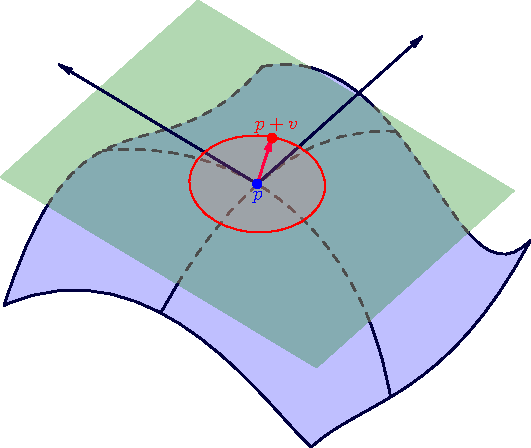
\includegraphics[width=.55\linewidth]{figures/N-20240413/tangent.pdf}
\caption{A tangent line is the first local linear model of a curve.}
\end{figure}

\section{The total derivative}

Let \(f:\mathbb R^n\to\mathbb R^m\). The total derivative at \(p\) is the linear map
\[
  Df_p:\mathbb R^n\to\mathbb R^m
\]
which best approximates \(f\) near \(p\):
\[
  f(p+h)=f(p)+Df_p(h)+o(\|h\|).
\]
The important word is \emph{linear}. Partial derivatives are not separate pieces of magic. They are the coordinates of this one linear map.

If \(f=(f_1,\ldots,f_m)\), the matrix of \(Df_p\) is the Jacobian
\[
  J_f(p)=
  \begin{bmatrix}
  \partial f_1/\partial x_1&\cdots&\partial f_1/\partial x_n\\
  \vdots&\ddots&\vdots\\
  \partial f_m/\partial x_1&\cdots&\partial f_m/\partial x_n
  \end{bmatrix}_{p}.
\]
So the derivative is not the matrix itself; the matrix is how the linear map looks after choosing coordinates.

\section{The chain rule as geometry}

If
\[
  \mathbb R^n\xrightarrow{f}\mathbb R^m\xrightarrow{g}\mathbb R^k,
\]
then
\[
  D(g\circ f)_p=Dg_{f(p)}\circ Df_p.
\]
This is the chain rule. In coordinates it becomes matrix multiplication, but the geometric meaning is simpler: local linear approximations compose.

\section{Tangent planes}

For a graph \(z=f(x,y)\), the tangent plane at \((a,b,f(a,b))\) is
\[
  z=f(a,b)+f_x(a,b)(x-a)+f_y(a,b)(y-b).
\]
This says that the graph is locally approximated by an affine plane whose direction is controlled by \(Df_{(a,b)}\).

For a level surface \(F(x,y,z)=c\), the tangent plane at \(p\) is
\[
  \nabla F(p)\cdot (X-p)=0.
\]
Here \(\nabla F(p)\) is normal to the surface. Again, the local geometry is encoded by a first derivative.

\section{Manifolds in one page}

A manifold is a space that may be curved globally but looks Euclidean locally. A chart is a coordinate system on a small open piece:
\[
  \varphi:U\to \mathbb R^n.
\]
An atlas is a collection of charts covering the space. The transition maps \(\psi\circ\varphi^{-1}\) compare coordinates on overlaps. If these transition maps are smooth, the manifold is a smooth manifold.

Examples include
\[
  S^1,\quad S^2,\quad T^2,\quad \mathbb{RP}^n,\quad \mathbb{CP}^n.
\]
Each is locally Euclidean, but none should be mistaken for a single Euclidean coordinate patch.

\section{Tangent vectors}

There are two useful pictures of tangent vectors. First, a tangent vector is the velocity of a curve:
\[
  v=\gamma'(0),\qquad \gamma(0)=p.
\]
Second, a tangent vector is a directional derivative acting on functions:
\[
  v(f)=\left.\frac{d}{dt}\right|_{t=0}f(\gamma(t)).
\]
The second viewpoint is more intrinsic. It does not require the manifold to sit inside a larger Euclidean space.

The tangent space \(T_pM\) is the vector space of tangent vectors at \(p\). A smooth map \(F:M\to N\) induces a linear map
\[
  dF_p:T_pM\to T_{F(p)}N.
\]
This is the manifold version of the total derivative.

\section{Regular values make manifolds}

Suppose \(F:\mathbb R^n\to\mathbb R^k\) is smooth. If \(c\) is a regular value, meaning \(DF_p\) is surjective for every \(p\in F^{-1}(c)\), then
\[
  F^{-1}(c)
\]
is a smooth manifold of dimension \(n-k\).

For example,
\[
  S^2=\{(x,y,z):x^2+y^2+z^2=1\}
\]
is the level set of \(F(x,y,z)=x^2+y^2+z^2\). Since \(\nabla F=2(x,y,z)\) never vanishes on \(S^2\), the sphere is a smooth surface.

%% expanded-on-review

\section{A worked example: polar coordinates}

Consider the coordinate map
\[
  F(r,\theta)=(r\cos\theta,r\sin\theta).
\]
Its derivative is
\[
  DF_{(r,\theta)}=
  \begin{bmatrix}
  \cos\theta&-r\sin\theta\\
  \sin\theta&r\cos\theta
  \end{bmatrix}.
\]
The two columns have a direct geometric meaning:
\[
  \frac{\partial F}{\partial r}=(\cos\theta,\sin\theta),
  \qquad
  \frac{\partial F}{\partial\theta}=(-r\sin\theta,r\cos\theta).
\]
The first vector points outward. The second vector points along the circle of radius \(r\). This is exactly what a coordinate system should do: it translates coordinate motion into actual tangent motion.

This example also explains why coordinate formulas can be misleading. The symbols \(\partial/\partial r\) and \(\partial/\partial\theta\) are coordinate directions, but after applying the derivative they become concrete tangent vectors in the plane.

\section{The tangent space of the sphere}

For the sphere
\[
  S^2=\{x\in\mathbb R^3:\|x\|^2=1\},
\]
the tangent space at \(p\in S^2\) is
\[
  T_pS^2=\{v\in\mathbb R^3:p\cdot v=0\}.
\]
This follows by differentiating the constraint \(x\cdot x=1\). If \(\gamma(t)\subset S^2\) and \(\gamma(0)=p\), then
\[
  \gamma(t)\cdot\gamma(t)=1.
\]
Differentiating at \(t=0\) gives
\[
  2p\cdot\gamma'(0)=0.
\]
So every velocity vector is perpendicular to the radius vector.

This calculation is a good model for many geometric arguments: start from an equation defining the space, differentiate the equation, and obtain the linear equation defining the tangent space.

\section{A small warning about coordinates}

A chart is a language. It is not the object itself. The same tangent vector can have different coordinate descriptions in different charts. What should remain unchanged is the geometric vector, not its coordinate list.

This is why differential geometry tries to separate intrinsic statements from coordinate expressions. Coordinates are useful for computation, but the real content is the object that survives changing coordinates.


\section{What to remember}

The derivative is the local linearization of geometry. The tangent space is the place where this linearization lives. A manifold is a space that allows this idea to be used locally everywhere.

The slogan is:
\[
\begin{array}{c}
  \text{calculus differentiates functions;}\\
  \text{geometry differentiates spaces.}
\end{array}
\]

\notechapter{N-20260304}{Point-Set Language in \texorpdfstring{$\mathbb R^n$}{Rn}: Neighborhoods, Open Sets, Closed Sets, and Compactness}


\section{Distance and neighborhoods}

For points $P_1=(a_1,\ldots,a_n)$ and $P_2=(b_1,\ldots,b_n)$ in $\mathbb R^n$, the Euclidean distance is
\[
  \rho(P_1,P_2)=\sqrt{\sum_{i=1}^n(a_i-b_i)^2}.
\]
Given $P_0\in\mathbb R^n$ and $\delta>0$, the open ball is
\[
  N_\delta(P_0)=\{P:\ \rho(P,P_0)<\delta\}.
\]

\section{Interior, exterior, boundary, and accumulation}

Let $E\subseteq\mathbb R^n$.  A point is interior to $E$ if some ball around it is contained in $E$; exterior if some ball is disjoint from $E$; and a boundary point if every ball meets both $E$ and its complement.  A point is an accumulation point if every punctured neighborhood contains a point of $E$.

The closure is $\overline E=E\cup E'$, where $E'$ is the set of accumulation points.  A set is closed iff it contains all its accumulation points, equivalently iff it contains limits of all convergent sequences from the set.

\section{Open, closed, bounded, and compact}

A set is open if every point is interior.  It is closed if its complement is open.  In $\mathbb R^n$, the Heine--Borel theorem says
\[
  K\text{ compact}\quad\Longleftrightarrow\quad K\text{ closed and bounded}.
\]
Compactness is the hidden reason why continuous functions on closed bounded regions attain maxima and minima.

\section{Connectedness}

A region in elementary multivariable calculus is often an open connected set, possibly together with its boundary.  Connectedness means the set cannot be split into two separated open pieces.  Path-connectedness means any two points can be joined by a continuous curve inside the set.

\section{Context and outlook}

Limits, continuity, differentiability, extrema, integration over domains, and change of variables all require control over how points approach a set.  Neighborhoods and boundaries are the grammar of multivariable analysis.



\paragraph{Expanded synthesis.}
The common theme of this chapter is that an elementary limiting or computational rule becomes powerful only after one specifies the space in which the limiting process takes place. The earlier sections (`Distance and neighborhoods`, `Interior, exterior, boundary, and accumulation`, `Open, closed, bounded, and compact`, `Connectedness`, `Higher viewpoint`) may look like separate techniques, but they all ask the same question: which operations are stable under approximation? A derivative is stable first-order approximation,
\[
  f(a+h)=f(a)+L(h)+o(|h|),
\]
while an integral is stable accumulation with respect to a measure, and a convergent series is a limit in a chosen norm or topology.

The advanced bridge is functional-analytic. Uniform convergence is convergence in a sup norm; $L^p$ convergence is convergence in an integral norm; differentiability is the existence of a continuous linear approximation; many differential equations are operator equations $L[u]=f$. Theorems such as dominated convergence, the inverse function theorem, the projection theorem in Hilbert spaces, and semigroup existence results are refined answers to the same elementary concern: when may we pass from finite approximations to a genuine limiting object?

To use this viewpoint when rereading the original examples, identify the hidden stability condition. A Taylor expansion asks for control of the remainder. A change of variables asks for differentiability and Jacobian control. Termwise differentiation of a series asks for uniform convergence of derivative series. A differential-equation formula asks whether the operator is invertible under the imposed initial or boundary data. The elementary computation is the visible part; the advanced theory names the hypotheses that make it legitimate.


\section{Expanded explanation: why point-set language is needed}

In one-variable calculus, most domains are intervals, so topology is hidden.  In several variables, domains may have holes, corners, boundary pieces, isolated points, or disconnected components.  The language of neighborhoods avoids relying on misleading pictures.

The most important definitions form a chain:
\[
  \text{interior}\quad\to\quad\text{open set}\quad\to\quad\text{limit point}\quad\to\quad\text{closed set}\quad\to\quad\text{compact set}.
\]
Each word controls a later theorem.

\section{Sequential tests and compactness}

A point $p$ lies in $\overline E$ iff there exists a sequence $(x_n)$ in $E$ with $x_n\to p$.  A set $E$ is closed iff every convergent sequence in $E$ has its limit in $E$.

Compactness is an existence machine.  If $K$ is compact and $f:K\to\mathbb R$ is continuous, then $f$ attains its maximum and minimum.  If $(x_n)$ is a sequence in compact $K$, it has a convergent subsequence.

\notechapter{N-20260306}{Multivariable Limits, Continuity, Differentiability, and the Total Derivative}


\section{Limits in several variables}

The statement $\lim_{(x,y)\to(x_0,y_0)}f(x,y)=A$ means that $f$ approaches $A$ along every possible approach to the point.  Checking only the two coordinate axes is not enough.  One either proves a uniform estimate in terms of $r=\sqrt{(x-x_0)^2+(y-y_0)^2}$, or disproves the limit by giving two paths with different limiting values.

\section{Continuity and partial derivatives}

Continuity at $P_0$ means
\[
  \lim_{P\to P_0}f(P)=f(P_0).
\]
The partial derivatives are
\[
\begin{aligned}
  f_x(x_0,y_0)&=\lim_{h\to0}\frac{f(x_0+h,y_0)-f(x_0,y_0)}h,\\
  f_y(x_0,y_0)&=\lim_{h\to0}\frac{f(x_0,y_0+h)-f(x_0,y_0)}h.
\end{aligned}
\]
They measure coordinate-direction changes.  Their existence alone does not imply continuity or differentiability.

\section{Differentiability as linear approximation}

The correct multivariable analogue of differentiability is the existence of a linear approximation:
\[
  f(P_0+h)=f(P_0)+L(h)+o(\|h\|).
\]
For scalar-valued $f$, the linear map is $L(h)=\nabla f(P_0)\cdot h$.  For $F:\mathbb R^n\to\mathbb R^m$, the derivative is the Jacobian matrix
\[
  DF(P_0)=\left(\frac{\partial F_i}{\partial x_j}(P_0)\right).
\]

\section{Directional derivatives and tangent planes}

For a unit vector $u$,
\[
  D_uf(P_0)=\lim_{t\to0}\frac{f(P_0+tu)-f(P_0)}t.
\]
If $f$ is differentiable, then $D_uf(P_0)=\nabla f(P_0)\cdot u$.  For a surface $z=f(x,y)$, the tangent plane is
\[
  z-z_0=f_x(x_0,y_0)(x-x_0)+f_y(x_0,y_0)(y-y_0).
\]
For $F(x,y,z)=0$, the tangent plane is $\nabla F(P_0)\cdot(P-P_0)=0$.




\section{Mixed partial derivatives as surface twist}

For a surface \(z=f(x,y)\), the mixed partial derivative
\[
  f_{xy}=\partial_x(\partial_y f)
\]
can be read geometrically as follows: first look at the slope of the \(y\)-direction tangent line, then ask how that slope changes as one moves in the \(x\)-direction.  Thus it measures a kind of local twisting of the surface rather than a new independent coordinate slope.

\begin{figure}[H]
\centering
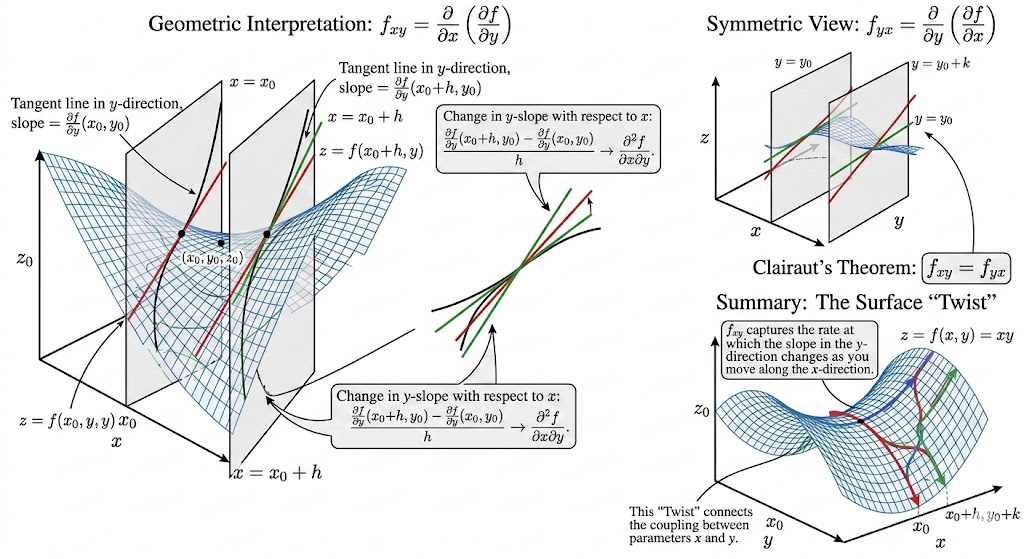
\includegraphics[width=0.94\textwidth,height=0.74\textheight,keepaspectratio]{figures/notes-md/N-20260306/N-20260306-fig-02-mixed-partial-derivative-geometric-interpretation.jpg}
\caption{Geometric interpretation of the mixed partial derivative: it measures how the \(y\)-direction slope changes as one moves in the \(x\)-direction, and symmetrically for \(f_{yx}\).}
\end{figure}

Under the usual smoothness hypotheses, Clairaut's theorem identifies the two orders:
\[
  f_{xy}=f_{yx}.
\]

\section{Expanded synthesis and advanced context}

Multivariable calculus replaces the slope of a line by a linear map.  Partial derivatives are its coordinate entries; the gradient is its vector representation in the scalar-valued case; the Jacobian is its matrix representation in the vector-valued case.



\paragraph{Expanded synthesis.}
For this chapter, the elementary material should be read as a study of what remains invariant when coordinates change. The earlier sections (`Limits in several variables`, `Continuity and partial derivatives`, `Differentiability as linear approximation`, `Directional derivatives and tangent planes`) compute with arrays, bases, pivots, determinants, or eigenvectors; the deeper object is a linear map together with the spaces it acts on. A matrix is a representation of that map after bases have been chosen. This is why formulas such as
\[
  A' = P^{-1}AP,\qquad \widetilde A = T^{-1}AS
\]
are not cosmetic: they distinguish an intrinsic morphism from a coordinate description.

The structural hierarchy is as follows. Kernels record what a map forgets, images record what it reaches, cokernels record obstructions to solvability, and quotients record information after an equivalence has been imposed. Determinants act on the top exterior power and therefore measure oriented volume; traces are invariant under cyclic rearrangement and become characters in representation theory; adjoints depend on an inner product and lead to self-adjoint spectral theory.

A useful way to return to the computations is to ask, for every formula, which invariant it is measuring. Row reduction measures rank and kernel; diagonalization measures decomposition into invariant subspaces; Gram--Schmidt measures orthogonal projection; positive definiteness measures ellipsoid geometry; tensor notation measures how components transform. The elementary methods are therefore the finite-dimensional laboratory in which duality, quotienting, functoriality, and spectral decomposition can be seen clearly.


\section{Expanded examples: why partial derivatives are not enough}

A standard counterexample is
\[
  f(x,y)=
  \begin{cases}
  \dfrac{xy}{x^2+y^2},&(x,y)\ne(0,0),\\
  0,&(x,y)=(0,0).
  \end{cases}
\]
Along the $x$-axis and $y$-axis the function is $0$, but along $y=x$ it tends to $1/2$.  Therefore the two-variable limit does not exist.

Another useful example is
\[
  f(x,y)=
  \begin{cases}
  \dfrac{x^2y}{x^4+y^2},&(x,y)\ne(0,0),\\
  0,&(x,y)=(0,0).
  \end{cases}
\]
Along every straight line $y=mx$ the limit is $0$, but along $y=x^2$ the limit is $1/2$.  This explains why checking only lines is not enough.

\section{Differentiability hierarchy}

The safe hierarchy is
\[
  C^1\Longrightarrow\text{differentiable}\Longrightarrow\text{continuous}.
\]
Existence of partial derivatives sits outside this chain unless additional hypotheses are imposed.  If the partial derivatives exist in a neighborhood and are continuous at the point, then the function is differentiable there.

\section{Frechet derivative viewpoint}

For $F:\mathbb R^n\to\mathbb R^m$, differentiability at $a$ means there is a linear map $L$ such that
\[
  \lim_{h\to0}\frac{|F(a+h)-F(a)-Lh|}{|h|}=0.
\]
The Jacobian matrix is merely the coordinate representation of $L$.  This formulation is the one that generalizes to Banach spaces.

\notechapter{N-20260313}{Multivariable Chain Rule, Total Derivatives, and Implicit Differentiation}


\section{Chain rule as matrix multiplication}

Let $F:\mathbb R^n\to\mathbb R^m$ and $G:\mathbb R^m\to\mathbb R^k$ be differentiable.  The derivative of the composite is
\[
  D(G\circ F)(x)=DG(F(x))\,DF(x).
\]
The familiar formulas with partial derivatives are coordinate expressions of this matrix multiplication.

For $z=f(u,v)$ with $u=\varphi(x)$ and $v=\psi(x)$,
\[
  \frac{dz}{dx}=\frac{\partial z}{\partial u}\frac{du}{dx}+\frac{\partial z}{\partial v}\frac{dv}{dx}.
\]
If $u=u(x,y)$ and $v=v(x,y)$, then
\[
  \frac{\partial z}{\partial x}=z_u u_x+z_v v_x,\qquad
  \frac{\partial z}{\partial y}=z_u u_y+z_v v_y.
\]

\section{Total differential}

The total differential packages first-order change:
\[
  dz=f_x\,dx+f_y\,dy.
\]
For a vector-valued map, the same idea becomes
\[
  dF=J_F\,dx,
\]
where $J_F$ is the Jacobian.  This notation is safe when interpreted as a linear approximation, not as a mysterious fraction manipulation.

\section{Implicit functions}

If $F(x,y)=0$ defines $y$ locally as a function of $x$ and $F_y\ne0$, then
\[
  \frac{dy}{dx}=-\frac{F_x}{F_y}.
\]
For a system $F(u,x)=0$ with $F_u$ invertible, the implicit derivative is
\[
  Du(x)=-(F_u)^{-1}F_x.
\]
This is the matrix form of solving the linearized constraint.

\section{Expanded synthesis and advanced context}

The chain rule is not a list of cases.  It says that first-order approximations compose.  The note's many formulas become conceptually simple once every derivative is viewed as a linear map and every chain rule as multiplication of those maps.



\paragraph{Expanded synthesis.}
For this chapter, the elementary material should be read as a study of what remains invariant when coordinates change. The earlier sections (`Chain rule as matrix multiplication`, `Total differential`, `Implicit functions`, `Higher viewpoint`, `Expanded chain-rule dictionary`) compute with arrays, bases, pivots, determinants, or eigenvectors; the deeper object is a linear map together with the spaces it acts on. A matrix is a representation of that map after bases have been chosen. This is why formulas such as
\[
  A' = P^{-1}AP,\qquad \widetilde A = T^{-1}AS
\]
are not cosmetic: they distinguish an intrinsic morphism from a coordinate description.

The structural hierarchy is as follows. Kernels record what a map forgets, images record what it reaches, cokernels record obstructions to solvability, and quotients record information after an equivalence has been imposed. Determinants act on the top exterior power and therefore measure oriented volume; traces are invariant under cyclic rearrangement and become characters in representation theory; adjoints depend on an inner product and lead to self-adjoint spectral theory.

A useful way to return to the computations is to ask, for every formula, which invariant it is measuring. Row reduction measures rank and kernel; diagonalization measures decomposition into invariant subspaces; Gram--Schmidt measures orthogonal projection; positive definiteness measures ellipsoid geometry; tensor notation measures how components transform. The elementary methods are therefore the finite-dimensional laboratory in which duality, quotienting, functoriality, and spectral decomposition can be seen clearly.


\section{Expanded chain-rule dictionary}

The note lists several chain-rule formulas.  They are all one formula in disguise.  If
\[
  x\mapsto (u(x),v(x))\mapsto z=f(u,v),
\]
then
\[
  \frac{dz}{dx}=
  \begin{pmatrix}f_u&f_v\end{pmatrix}
  \begin{pmatrix}u_x\\v_x\end{pmatrix}.
\]
If $(x,y)\mapsto(u,v)\mapsto z$, then
\[
  \begin{pmatrix}z_x&z_y\end{pmatrix}
  =
  \begin{pmatrix}f_u&f_v\end{pmatrix}
  \begin{pmatrix}u_x&u_y\\v_x&v_y\end{pmatrix}.
\]
This is exactly Jacobian multiplication.

\section{Implicit differentiation as solving a linearized constraint}

For $F(x,y)=0$, differentiating gives
\[
  F_x\,dx+F_y\,dy=0.
\]
If $F_y\ne0$, then
\[
  \frac{dy}{dx}=-\frac{F_x}{F_y}.
\]
For a system $F(x,u)=0$, the same argument gives
\[
  du=-F_u^{-1}F_x\,dx.
\]
The implicit function theorem says when this linearized computation is locally legitimate.

\notechapter{N-20260314}{A Cookbook for Multivariable Topology, Limits, and Differential Computations}


\section{Classifying points relative to a set}

For a set $G\subseteq\mathbb R^n$, classify a point $P$ by inspecting small balls around it.  If some ball lies inside $G$, $P$ is interior.  If some ball is disjoint from $G$, $P$ is exterior.  If every ball meets both $G$ and $G^c$, $P$ is a boundary point.  This is the fastest way to understand open, closed, and neither-open-nor-closed examples.

\section{Limits}

To prove a multivariable limit, dominate the expression by a function of $r=\|x-a\|$ going to zero.  To disprove it, use two paths.  Polar coordinates are useful near the origin because they separate radial size from angular dependence:
\[
  x=r\cos\theta,\qquad y=r\sin\theta.
\]
If a candidate expression becomes $r^\alpha g(\theta)$ with bounded $g$ and $\alpha>0$, the limit is zero.

\section{Differentiability and tangent objects}

The standard hierarchy is
\[
  C^1\Rightarrow\text{differentiable}\Rightarrow\text{continuous}\Rightarrow\text{directional limits behave well in value}.
\]
The reverse implications usually fail.  Tangent lines, normal lines, and tangent planes are all first-order approximations.  For $F(x,y,z)=0$, the normal vector is $\nabla F$; for $z=f(x,y)$, the tangent plane comes from the differential $dz=f_xdx+f_ydy$.

\section{Expanded synthesis and advanced context}

A cookbook is useful only if it remembers why the recipes work.  The recipes here are all forms of one idea: replace a complicated local object by its simplest stable approximation, either a ball for topology, a radial estimate for limits, or a linear map for differentiability.



\paragraph{Expanded synthesis.}
For this chapter, the elementary material should be read as a study of what remains invariant when coordinates change. The earlier sections (`Classifying points relative to a set`, `Limits`, `Differentiability and tangent objects`, `Higher viewpoint`, `Expanded cookbook with failure modes`) compute with arrays, bases, pivots, determinants, or eigenvectors; the deeper object is a linear map together with the spaces it acts on. A matrix is a representation of that map after bases have been chosen. This is why formulas such as
\[
  A' = P^{-1}AP,\qquad \widetilde A = T^{-1}AS
\]
are not cosmetic: they distinguish an intrinsic morphism from a coordinate description.

The structural hierarchy is as follows. Kernels record what a map forgets, images record what it reaches, cokernels record obstructions to solvability, and quotients record information after an equivalence has been imposed. Determinants act on the top exterior power and therefore measure oriented volume; traces are invariant under cyclic rearrangement and become characters in representation theory; adjoints depend on an inner product and lead to self-adjoint spectral theory.

A useful way to return to the computations is to ask, for every formula, which invariant it is measuring. Row reduction measures rank and kernel; diagonalization measures decomposition into invariant subspaces; Gram--Schmidt measures orthogonal projection; positive definiteness measures ellipsoid geometry; tensor notation measures how components transform. The elementary methods are therefore the finite-dimensional laboratory in which duality, quotienting, functoriality, and spectral decomposition can be seen clearly.


\section{Expanded cookbook with failure modes}

A cookbook is useful only when each recipe includes its failure mode.

For limits, path testing can disprove a limit but cannot prove it unless all paths are covered by an estimate.  For continuity, partial continuity in each variable is necessary but insufficient.  For differentiability, existence of all directional derivatives is also insufficient unless they assemble into a linear approximation.

\section{Practical limit templates}

Near the origin, convert to polar coordinates when the expression is homogeneous or nearly homogeneous.  If
\[
  f(r\cos\theta,r\sin\theta)=r^\alpha g(\theta)
\]
with $\alpha>0$ and bounded $g$, then the limit is zero.  If $g(\theta)$ remains in the limit with no decaying factor, the limit depends on direction.

For rational expressions, compare total degrees.  If the numerator has strictly higher degree than the denominator and the denominator is comparable to a power of $r$, the limit is often zero.  But cancellations and anisotropic denominators require care.

\section{Tangent and normal templates}

For $z=f(x,y)$, use the graph formula.  For $F(x,y,z)=0$, use the gradient.  For a space curve given as the intersection of $F=0$ and $G=0$, the tangent direction is
\[
  \nabla F\times \nabla G.
\]
This follows because the tangent vector must be perpendicular to both normals.

\notechapter{N-20260325}{Extrema of Two-Variable Functions and the Hessian Test}


\section{Local extrema}

For $f(x,y)$ defined on a region $G$, a point $P_0\in G$ is a local maximum if $f(P)\le f(P_0)$ for all $P$ near $P_0$, and a local minimum if $f(P)\ge f(P_0)$.  If the inequality is strict away from $P_0$, the extremum is strict.

\section{Necessary condition}

If $f$ is differentiable at an interior local extremum, then
\[
  \nabla f(P_0)=0.
\]
This is Fermat's theorem in several variables: every directional derivative must vanish.  Such points are critical points, but not every critical point is an extremum.

\section{Second derivative test}

Let
\[
  A=f_{xx}(P_0),\qquad B=f_{xy}(P_0),\qquad C=f_{yy}(P_0),\qquad D=AC-B^2.
\]
If $\nabla f(P_0)=0$, then:
\[
\begin{aligned}
  D>0,\ A>0&\Rightarrow\text{local minimum},\\
  D>0,\ A<0&\Rightarrow\text{local maximum},\\
  D<0&\Rightarrow\text{saddle point}.
\end{aligned}
\]
If $D=0$, the test is inconclusive.  This is the quadratic form test for the Hessian matrix.

\section{Constrained extrema}

For a constraint $g(x,y)=0$, the Lagrange multiplier condition is
\[
  \nabla f=\lambda \nabla g.
\]
Geometrically, at a constrained extremum the level curve of $f$ is tangent to the constraint curve.  For several constraints, the gradient of $f$ lies in the span of the constraint gradients.

\section{Expanded synthesis and advanced context}

The first derivative locates candidates; the second derivative classifies the local quadratic model.  Unconstrained extrema are about the Hessian; constrained extrema are about tangency of level sets.



\paragraph{Expanded synthesis.}
For this chapter, the elementary material should be read as a study of what remains invariant when coordinates change. The earlier sections (`Local extrema`, `Necessary condition`, `Second derivative test`, `Constrained extrema`, `Higher viewpoint`) compute with arrays, bases, pivots, determinants, or eigenvectors; the deeper object is a linear map together with the spaces it acts on. A matrix is a representation of that map after bases have been chosen. This is why formulas such as
\[
  A' = P^{-1}AP,\qquad \widetilde A = T^{-1}AS
\]
are not cosmetic: they distinguish an intrinsic morphism from a coordinate description.

The structural hierarchy is as follows. Kernels record what a map forgets, images record what it reaches, cokernels record obstructions to solvability, and quotients record information after an equivalence has been imposed. Determinants act on the top exterior power and therefore measure oriented volume; traces are invariant under cyclic rearrangement and become characters in representation theory; adjoints depend on an inner product and lead to self-adjoint spectral theory.

A useful way to return to the computations is to ask, for every formula, which invariant it is measuring. Row reduction measures rank and kernel; diagonalization measures decomposition into invariant subspaces; Gram--Schmidt measures orthogonal projection; positive definiteness measures ellipsoid geometry; tensor notation measures how components transform. The elementary methods are therefore the finite-dimensional laboratory in which duality, quotienting, functoriality, and spectral decomposition can be seen clearly.


\section{Expanded Hessian interpretation}

At a critical point, the Taylor expansion begins as
\[
  f(P_0+h)=f(P_0)+\frac12 h^T H(P_0)h+o(|h|^2).
\]
Thus the classification problem becomes classification of the quadratic form $h^THh$.

For two variables,
\[
  H=\begin{pmatrix}A&B\\B&C\end{pmatrix},\qquad D=AC-B^2.
\]
If $D>0$ and $A>0$, then $H$ is positive definite; if $D>0$ and $A<0$, it is negative definite; if $D<0$, it takes both signs, so the point is a saddle.

\section{Constrained extrema and geometry}

For $g(x,y)=0$, the gradient $\nabla g$ is normal to the constraint curve.  At a constrained extremum, moving along the curve produces no first-order change in $f$, so $\nabla f$ must also be normal to the curve.  Hence
\[
  \nabla f=\lambda\nabla g.
\]
The multiplier $\lambda$ records sensitivity of the extremal value to relaxing the constraint.



\part{Integration and Vector Fields}
\label{vol:10-integration-and-vector-fields}
\begingroup
\small
\sloppy
\parttoc
\endgroup

% This file is generated during volume reorganization.
% Volume: Integration and Vector Fields

\notechapter{N-20230123}{Definite Integrals, Line Integrals, Work, Green-Type Thinking, and Vector Operations}

\section{Indefinite and definite integrals}

The note begins by distinguishing indefinite and definite integrals.  An indefinite integral is an antiderivative family:
\[
  \int f(x)\,dx=F(x)+C,\qquad F'(x)=f(x).
\]
A definite integral is a number:
\[
  \int_a^b f(x)\,dx.
\]
Geometrically, it is signed area under the graph.  Analytically, it is the limit of Riemann sums.

The fundamental theorem of calculus connects the two:
\[
  \int_a^b f(x)\,dx=F(b)-F(a)
\]
when $F'=f$.

\section{Area by slicing}

The page includes diagrams of shaded regions.  The standard method is to slice a region into thin strips.  If vertical strips are convenient, then
\[
  A=\int_a^b (y_{top}(x)-y_{bottom}(x))\,dx.
\]
If horizontal strips are more convenient, then
\[
  A=\int_c^d (x_{right}(y)-x_{left}(y))\,dy.
\]
The note's sketches show that choosing the direction of slicing is part of the solution, not a fixed rule.

\section{Work as an integral}

The physical meaning of a definite integral appears in work.  If a force $F(x)$ acts along a line, then the work from $x=a$ to $x=b$ is
\[
  W=\int_a^b F(x)\,dx.
\]
If the force is constant, this reduces to $W=F(b-a)$.  If the force changes with position, integration adds the small contributions
\[
  dW=F(x)\,dx.
\]
This is the same accumulation idea as area, but with a physical interpretation.

\section{Line integrals}

The note then introduces line integrals.  If a curve is parametrized by
\[
  r(t)=(x(t),y(t)),\qquad a\le t\le b,
\]
then the scalar line element is
\[
  ds=\sqrt{(x'(t))^2+(y'(t))^2}\,dt.
\]
A scalar line integral is
\[
  \int_C f\,ds
  =\int_a^b f(x(t),y(t))\sqrt{(x'(t))^2+(y'(t))^2}\,dt.
\]
For a vector field $F=(P,Q)$, the work integral is
\[
  \int_C F\cdot dr
  =\int_C P\,dx+Q\,dy
  =\int_a^b [P(x(t),y(t))x'(t)+Q(x(t),y(t))y'(t)]\,dt.
\]

\section{Green-type intuition}

The handwritten diagrams show a small oriented boundary and a vector field.  The idea is that circulation around a boundary can be related to a double integral over the region.  In the plane, Green's theorem says
\[
  \oint_{\partial D} P\,dx+Q\,dy
  =
  \iint_D \left(\frac{\partial Q}{\partial x}-\frac{\partial P}{\partial y}\right)\,dA.
\]
Even if the note does not prove the theorem fully, it records the key intuition: local rotation accumulated over an area produces circulation on the boundary.

\section{Polar coordinates}

The note uses polar coordinates in examples.  The change of variables is
\[
  x=r\cos\theta,\qquad y=r\sin\theta.
\]
The area element becomes
\[
  dA=r\,dr\,d\theta.
\]
The factor $r$ is the Jacobian.  Geometrically, a small polar rectangle has side lengths approximately $dr$ and $r\,d\theta$.

Thus a disk of radius $R$ has area
\[
  \int_0^{2\pi}\int_0^R r\,dr\,d\theta=\pi R^2.
\]

\section{Spherical coordinates}

The later page contains a spherical-coordinate diagram.  A common convention is
\[
  x=\rho\sin\varphi\cos\theta,\qquad
  y=\rho\sin\varphi\sin\theta,\qquad
  z=\rho\cos\varphi.
\]
The volume element is
\[
  dV=\rho^2\sin\varphi\,d\rho\,d\varphi\,d\theta.
\]
The factor $\rho^2\sin\varphi$ comes from the three small lengths:
\[
  d\rho,\qquad \rho\,d\varphi,\qquad \rho\sin\varphi\,d\theta.
\]
This explains the diagram on the final page: the small spherical patch has dimensions determined by radius and angle.

\section{Dot product and cross product}

The note also summarizes vector operations.  The dot product is
\[
  a\cdot b=|a||b|\cos\theta.
\]
It measures projection and appears in work:
\[
  dW=F\cdot dr.
\]
The cross product has magnitude
\[
  |a\times b|=|a||b|\sin\theta
\]
and direction given by orientation.  It measures the area of the parallelogram spanned by $a$ and $b$.

In coordinates,
\[
  a\times b=
  \begin{vmatrix}
  i&j&k\\
  a_1&a_2&a_3\\
  b_1&b_2&b_3
  \end{vmatrix}.
\]

\section{Expanded synthesis and advanced context}

The note develops integration as accumulation in increasingly geometric forms.  Ordinary definite integrals accumulate along a line.  Line integrals accumulate along a curve.  Double and triple integrals accumulate over area and volume.  Coordinate changes require Jacobians.  Dot products, cross products, and differential elements provide the language for physical quantities such as work, flux, and circulation.



\paragraph{Expanded synthesis.}
For this chapter, the elementary material should be read as a study of what remains invariant when coordinates change. The earlier sections (`Indefinite and definite integrals`, `Area by slicing`, `Work as an integral`, `Line integrals`, `Green-type intuition`) compute with arrays, bases, pivots, determinants, or eigenvectors; the deeper object is a linear map together with the spaces it acts on. A matrix is a representation of that map after bases have been chosen. This is why formulas such as
\[
  A' = P^{-1}AP,\qquad \widetilde A = T^{-1}AS
\]
are not cosmetic: they distinguish an intrinsic morphism from a coordinate description.

The structural hierarchy is as follows. Kernels record what a map forgets, images record what it reaches, cokernels record obstructions to solvability, and quotients record information after an equivalence has been imposed. Determinants act on the top exterior power and therefore measure oriented volume; traces are invariant under cyclic rearrangement and become characters in representation theory; adjoints depend on an inner product and lead to self-adjoint spectral theory.

A useful way to return to the computations is to ask, for every formula, which invariant it is measuring. Row reduction measures rank and kernel; diagonalization measures decomposition into invariant subspaces; Gram--Schmidt measures orthogonal projection; positive definiteness measures ellipsoid geometry; tensor notation measures how components transform. The elementary methods are therefore the finite-dimensional laboratory in which duality, quotienting, functoriality, and spectral decomposition can be seen clearly.


\section{Elementary-to-advanced bridge: line integrals as pullbacks}

For a parametrized curve $\gamma:[a,b]\to\mathbb R^n$, a line integral of a one-form
\[
  \omega=P_1dx_1+\cdots+P_ndx_n
\]
is
\[
  \int_\gamma \omega
  =\int_a^b \sum_i P_i(\gamma(t))\gamma_i'(t)\,dt.
\]
This is the pullback of the one-form to the interval:
\[
  \gamma^*\omega=\sum_i P_i(\gamma(t))\gamma_i'(t)dt.
\]
Thus the elementary formula $Pdx+Qdy$ is already differential-form notation.

\section{Elementary-to-advanced bridge: exact forms and potentials}

A one-form $\omega$ is exact if $\omega=df$ for some potential $f$.  Then
\[
  \int_\gamma df=f(\gamma(b))-f(\gamma(a)).
\]
This is the fundamental theorem of line integrals.

A form is closed if $d\omega=0$.  In the plane, for $\omega=Pdx+Qdy$, this means
\[
  Q_x-P_y=0.
\]
On simply connected domains, closed one-forms are exact.  On domains with holes, this may fail.

\section{Elementary-to-advanced bridge: conservation laws}

In mechanics, work is a line integral
\[
  W=\int_C F\cdot dr.
\]
If $F=-\nabla V$ is conservative, then
\[
  W=V(A)-V(B)
\]
depends only on endpoints.  Conservation of energy is therefore a statement about exact one-forms.

This connects elementary work integrals to topology: path independence is not only about derivatives; it also depends on whether the domain has holes.

\section{Elementary-to-advanced bridge: de Rham preview}

De Rham cohomology measures the failure of closed forms to be exact:
\[
  H^1_{dR}(M)=\frac{\{\text{closed 1-forms}\}}{\{\text{exact 1-forms}\}}.
\]
For the punctured plane, the form
\[
  \omega=\frac{-y\,dx+x\,dy}{x^2+y^2}
\]
is closed but not exact.  Its integral around the unit circle is $2\pi$.

The elementary line integral around a circle is therefore a measurement of a topological hole.

% Second-pass deepening for waves 2-4: wave 4 part 2
\section{Second-pass deepening: work integrals and gauge freedom}

If a force field is conservative, $F=-\nabla V$, then work depends only on endpoints.  The potential $V$ is not unique: adding a constant changes nothing.  This is the simplest form of gauge freedom.  The physically meaningful object is the differential $dV$, not the absolute zero of potential.

In electromagnetism, potentials have richer gauge freedom.  A vector potential $A$ may be changed by a gradient without changing the magnetic field $B=\nabla\times A$.  The elementary fact that potentials are determined only up to constants is the first example of this broader principle.

\section{Second-pass deepening: polar and spherical coordinates as adapted charts}

The original integral examples using polar or spherical coordinates should be read as choosing charts adapted to symmetry.  A chart is a coordinate map from a parameter domain to the geometric region.  The integration element is obtained by pulling back the metric or volume form.

Thus polar coordinates are not merely a trick for circular regions.  They are a coordinate chart on the punctured plane adapted to the action of rotations.  Spherical coordinates are adapted to radial symmetry in three dimensions.

\notechapter{N-20230201}{Gravitational Field inside a Uniform Spherical Shell}

\section{Problem}

The note studies the classical shell theorem: the gravitational field produced by a uniform spherical shell at any interior point is zero.  The physical statement is simple, but the proof is a good training ground for geometric integration.

Let the shell have surface density \(\sigma\), center \(O\), and let \(P\) be an interior point.  We want to prove that the total gravitational field at \(P\) cancels.

\section{Geometric pairing method}

Choose the axis \(OP\).  A ray through \(P\) meets the sphere in two opposite small surface elements.  Although one element is farther away than the other, it also subtends a correspondingly larger area.  The inverse-square law and the area scaling cancel exactly.

\begin{figure}[H]
\centering
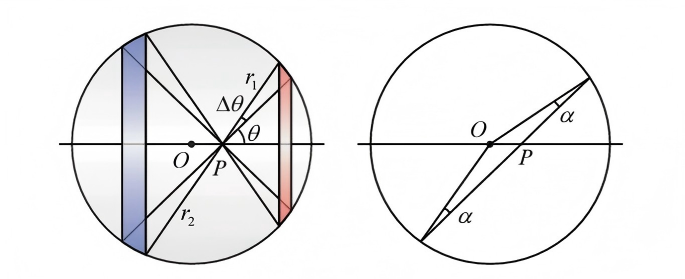
\includegraphics[width=.72\linewidth]{figures/N-20230201/01-shell-geometric-method.png}
\caption{Opposite surface elements seen from an interior point.}
\end{figure}

The note writes the masses of two corresponding small rings or patches as proportional to their areas.  If their distances from \(P\) are \(r_1,r_2\), then the gravitational magnitudes contain factors of the form
\[
  \frac{G\,dM_i}{r_i^2}.
\]
But \(dM_i\) itself is proportional to \(r_i^2\) times the same solid angle.  Therefore the two fields have equal magnitudes and opposite directions.  Pairing all such opposite elements gives total field zero.

This is the cleanest idea: the inverse-square law is exactly matched by the square scaling of area under fixed solid angle.

\section{Integral method}

The note also gives an integration method.  Let the field point be at distance \(r\) from the center.  A circular ring on the shell at polar angle \(\theta\) has mass
\[
  dM=2\pi R^2\sigma\sin\theta\,d\theta.
\]
The contribution along the axis is
\[
  dg=\frac{G\,dM}{\ell^2}\cos\alpha,
\]
where \(\ell\) is the distance from the ring to \(P\) and \(\alpha\) is the angle between the line of force and the axis.

\begin{figure}[H]
\centering
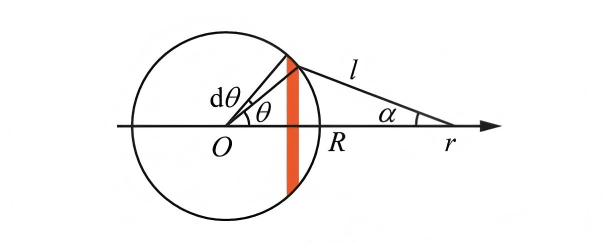
\includegraphics[width=.62\linewidth]{figures/N-20230201/02-shell-integral-method.png}
\caption{Ring integration for the field of a spherical shell.}
\end{figure}

Using the law of cosines and differentiating the relation between \(\ell\) and \(\theta\), the integral collapses to zero for \(r<R\).  The algebra is less transparent than the pairing proof, but it is more systematic and generalizes to other symmetric mass distributions.

\section{Connection with Newton's theorem}

The theorem has two parts:
\begin{enumerate}[(i)]
  \item outside a uniform spherical shell, the field is as if all mass were concentrated at the center;
  \item inside the shell, the field is zero.

\end{enumerate}
The note focuses on the second.  For a solid uniform ball, the interior field at radius \(r\) depends only on the mass inside radius \(r\), because outer spherical shells contribute zero.  Thus
\[
  g(r)=\frac{G M(r)}{r^2}\propto r
\]
inside a uniform solid sphere.


\section{Details of the solid-angle argument}

The pairing proof deserves more detail.  From the interior point \(P\), take a very small cone of solid angle \(d\Omega\).  It cuts two small patches from the spherical shell, one on the near side and one on the far side.  If their distances from \(P\) are \(r_1\) and \(r_2\), then the corresponding patch areas are, up to the same obliquity factor,
\[
  dS_i\propto r_i^2\,d\Omega .
\]
Their masses are \(dM_i=\sigma dS_i\).  The gravitational acceleration produced by each patch has magnitude
\[
  dg_i=G\frac{dM_i}{r_i^2}.
\]
The factor \(r_i^2\) in area cancels the inverse-square law.  The two patches lie in opposite directions along the same line through \(P\), so their vector contributions cancel.

This is the core reason the theorem is true.  It is not merely symmetry around the center of the sphere; the point \(P\) is not at the center.  The cancellation works because the inverse-square law exactly matches how apparent area scales with distance.

\section{Why the theorem would fail for a different force law}

If the force were proportional to \(1/r^3\) or \(1/r\), the same cancellation would not occur.  The near and far patches would still subtend the same solid angle, but their masses would scale like \(r^2\), while the force factor would scale differently.  Thus the shell theorem is a special consequence of the inverse-square law.

This also explains why the result is closely related to Gauss's law.  Inverse-square fields have constant flux through spheres.  A spherical shell contributes zero field inside because a Gaussian sphere inside the shell encloses no mass.

\section{Potential viewpoint}

Another way to understand the theorem is through gravitational potential.  The potential of a shell at an interior point is constant.  Since gravitational field is the negative gradient of potential,
\[
  \mathbf g=-\nabla V,
\]
a constant potential inside implies zero field.

This viewpoint is often cleaner in advanced mechanics: instead of adding vector forces directly, compute a scalar potential and then differentiate.  It also connects the shell theorem with harmonic functions and Laplace's equation.

\section{Expanded synthesis and advanced context}

The shell theorem is an early example of symmetry plus inverse-square law.  In modern language, it is closely related to Gauss's law: a spherically symmetric field has flux controlled by enclosed mass.  The geometric proof shows why the exponent \(2\) is special; the integral proof shows how symmetry reduces a surface integral to one variable.


\paragraph{Expanded synthesis.}
The common theme of this chapter is that an elementary limiting or computational rule becomes powerful only after one specifies the space in which the limiting process takes place. The earlier sections (`Problem`, `Geometric pairing method`, `Integral method`, `Connection with Newton's theorem`, `Details of the solid-angle argument`) may look like separate techniques, but they all ask the same question: which operations are stable under approximation? A derivative is stable first-order approximation,
\[
  f(a+h)=f(a)+L(h)+o(|h|),
\]
while an integral is stable accumulation with respect to a measure, and a convergent series is a limit in a chosen norm or topology.

The advanced bridge is functional-analytic. Uniform convergence is convergence in a sup norm; $L^p$ convergence is convergence in an integral norm; differentiability is the existence of a continuous linear approximation; many differential equations are operator equations $L[u]=f$. Theorems such as dominated convergence, the inverse function theorem, the projection theorem in Hilbert spaces, and semigroup existence results are refined answers to the same elementary concern: when may we pass from finite approximations to a genuine limiting object?

To use this viewpoint when rereading the original examples, identify the hidden stability condition. A Taylor expansion asks for control of the remainder. A change of variables asks for differentiability and Jacobian control. Termwise differentiation of a series asks for uniform convergence of derivative series. A differential-equation formula asks whether the operator is invertible under the imposed initial or boundary data. The elementary computation is the visible part; the advanced theory names the hypotheses that make it legitimate.

\notechapter{N-20230311}{Riemann Integration and Lebesgue Integration: From Partitions of the Domain to Partitions of Values}

\section{Why two theories of integration exist}

This note compares Riemann integration and Lebesgue integration.  A compressed summary such as “Riemann cuts the $x$-axis; Lebesgue cuts the $y$-axis” is memorable, but it is not enough.  The real issue is what kinds of limiting processes the integral is supposed to tolerate.

Riemann integration works beautifully for continuous functions and many functions with mild discontinuities.  But once functions oscillate too much, especially when rational and irrational points behave differently, the Riemann approach becomes rigid.  Lebesgue integration was designed to handle limits of functions more naturally, especially in analysis, probability, and Fourier theory.

\section{Riemann sums}

Let $f:[a,b]\to\mathbb R$ be bounded.  A partition is a finite sequence
\[
  P:a=x_0<x_1<\cdots<x_n=b.
\]
Choose a sample point $\xi_i\in[x_{i-1},x_i]$ in each subinterval.  The Riemann sum is
\[
  \sum_{i=1}^n f(\xi_i)\Delta x_i,
  \qquad
  \Delta x_i=x_i-x_{i-1}.
\]
If all such sums approach the same limit as the mesh
\[
  \|P\|=\max_i \Delta x_i
\]
tends to zero, that limit is the Riemann integral.

The geometric picture is rectangles under a graph.  But the definition is not simply about drawing rectangles; it says that the total contribution should stabilize no matter how the sample points are chosen, once the partition is sufficiently fine.

\section{Darboux upper and lower sums}

A cleaner equivalent formulation is Darboux integration.  On each interval $[x_{i-1},x_i]$, define
\[
  M_i=\sup_{x\in[x_{i-1},x_i]} f(x),
  \qquad
  m_i=\inf_{x\in[x_{i-1},x_i]} f(x).
\]
The upper and lower sums are
\[
  U(P,f)=\sum_i M_i\Delta x_i,
  \qquad
  L(P,f)=\sum_i m_i\Delta x_i.
\]
Then
\[
  f\text{ is Riemann integrable}
  \quad\Longleftrightarrow\quad
  \inf_P U(P,f)=\sup_P L(P,f).
\]
The common value is the integral.

This formulation explains why discontinuities matter.  If a function oscillates wildly on every interval, then $M_i-m_i$ remains large no matter how small the interval is, and the upper and lower sums cannot meet.

\section{A simple integrable discontinuity}

Consider
\[
  f(x)=\begin{cases}
  1,&x=c,\\
  0,&x\ne c
  \end{cases}
\]
on $[a,b]$.  This function is discontinuous at one point, but it is Riemann integrable with integral zero.  Indeed, the lower sums are all zero.  For any partition, only one subinterval can contain $c$, and the contribution to the upper sum from that subinterval can be made arbitrarily small.

Thus Riemann integration tolerates finite discontinuities.  More generally, a bounded function is Riemann integrable iff its set of discontinuities has Lebesgue measure zero.  This theorem already hints that measure theory is hiding behind Riemann integration.

\section{Dirichlet's function}

The Dirichlet function is
\[
  1_{\mathbb Q}(x)=\begin{cases}
  1,&x\in\mathbb Q,\\
  0,&x\notin\mathbb Q.
  \end{cases}
\]
On every nonempty interval there are rational and irrational numbers.  Therefore on every subinterval,
\[
  M_i=1,
  \qquad
  m_i=0.
\]
Hence
\[
  U(P,f)=b-a,
  \qquad
  L(P,f)=0
\]
for every partition.  The upper and lower integrals never meet, so the function is not Riemann integrable.

Lebesgue integration handles this example immediately: since $\mathbb Q$ is countable and has measure zero,
\[
  \int_{[a,b]}1_{\mathbb Q}\,dx=0.
\]
This one example explains much of the motivation for Lebesgue's theory.

\section{The Lebesgue idea}

Riemann integration partitions the domain into small intervals and asks how the function behaves on each interval.  Lebesgue integration partitions according to values.  For a nonnegative simple function
\[
  s=\sum_{j=1}^m a_j1_{E_j},
\]
where the $E_j$ are measurable and disjoint, define
\[
  \int s\,d\mu=\sum_{j=1}^m a_j\mu(E_j).
\]
For a nonnegative measurable function $f$, define
\[
  \int f\,d\mu=\sup\left\{\int s\,d\mu:s\le f,\ s\text{ simple}\right\}.
\]
For a general integrable function, write
\[
  f=f^+-f^-.
\]
If both $\int f^+$ and $\int f^-$ are finite, define
\[
  \int f=\int f^+-\int f^-.
\]

The construction is less pictorial than Riemann sums, but more robust.  It counts how much space is occupied by each range of values.

\section{Characteristic functions and sets}

The Lebesgue integral turns set measure into function integration:
\[
  \int 1_E\,d\mu=\mu(E).
\]
This is conceptually important.  Sets become functions, and measuring a set becomes integrating its indicator.  Probability theory uses exactly this viewpoint: expectation is integration, and probabilities are integrals of indicators.

For the Dirichlet function,
\[
  1_{\mathbb Q\cap[a,b]}
\]
has integral zero because the rationals are countable.  For the Thomae function, which is discontinuous at every rational and continuous at every irrational, the function is still Riemann integrable because its discontinuity set is countable.  Lebesgue theory makes such examples easier to organize.

\section{Convergence theorems}

The major advantage of Lebesgue integration is not merely that it integrates more functions.  It has powerful limit theorems.

The Monotone Convergence Theorem says: if
\[
  0\le f_1\le f_2\le\cdots,
  \qquad
  f_n\to f,
\]
then
\[
  \int f\,d\mu=\lim_{n\to\infty}\int f_n\,d\mu.
\]
The Dominated Convergence Theorem says: if $f_n\to f$ pointwise, and $|f_n|\le g$ for an integrable $g$, then
\[
  \lim_{n\to\infty}\int f_n\,d\mu=\int f\,d\mu.
\]
These are theorems Riemann integration cannot match in such generality.  They explain why Lebesgue integration becomes the standard language of modern analysis.

\section{Improper Riemann integrals versus Lebesgue integrals}

A subtle point: some improper Riemann integrals converge conditionally but are not Lebesgue integrable.  For example,
\[
  \int_1^\infty \frac{\sin x}{x}\,dx
\]
converges as an improper integral, but
\[
  \int_1^\infty \left|\frac{\sin x}{x}\right|dx
\]
diverges.  Lebesgue integrability of a signed function requires integrability of the absolute value.  Thus Lebesgue integration is not simply “more permissive”; it is more structurally consistent with normed function spaces such as $L^1$.

\section{Comparison table}

\begin{center}
\small
\begin{tabularx}{\textwidth}{@{}lYY@{}}
\toprule
Aspect & Riemann & Lebesgue \\
\midrule
Partition & Domain intervals & Value levels and measurable sets \\
Basic object & Bounded functions on intervals & Measurable functions \\
Bad example & $1_{\mathbb Q}$ not integrable & Integral is $0$ \\
Limit theorems & Limited & MCT, Fatou, DCT \\
Natural space & Continuous functions and elementary calculus & $L^p$ spaces, probability, Fourier analysis \\
\bottomrule
\end{tabularx}
\end{center}


\section{Source repair: the measure-space starting point}

The uploaded note explicitly starts the Lebesgue construction from a measure space
\[
  (X,\mathcal M,\mu),
\]
where \(\mathcal M\) is a \(\sigma\)-algebra and \(\mu\) is a measure.  A function \(f:X\to\mathbb R\) is measurable if sets such as
\[
  \{x\in X:f(x)>\alpha\}
\]
belong to \(\mathcal M\) for every real \(\alpha\).  This is the point at which the theory leaves elementary calculus: before integrating, one must decide which subsets are measurable.

\section{Source repair: simple functions as building blocks}

The uploaded text defines a nonnegative simple function by
\[
  \varphi(x)=\sum_{i=1}^n a_i\chi_{A_i}(x),
\]
and sets
\[
  \int_X \varphi\,d\mu=\sum_{i=1}^n a_i\mu(A_i).
\]
For a nonnegative measurable function,
\[
  \int_X f\,d\mu
  =\sup\left\{\int_X\varphi\,d\mu:0\le\varphi\le f,\ \varphi\text{ simple}\right\}.
\]
This is the formal version of cutting by values.  Instead of approximating the domain by small intervals, we approximate the function from below by simple measurable functions.

\section{Source repair: probability viewpoint}

The source also points toward probability.  A random variable is a measurable function, and expectation is an integral:
\[
  \mathbb E[X]=\int_\Omega X\,d\mathbb P.
\]
Events are measured by probabilities, and indicators satisfy
\[
  \mathbb E[1_A]=\mathbb P(A).
\]
This makes the Lebesgue framework the natural language of modern probability, not only a generalization of calculus.

\section{A note on scope}

The slogan is useful:
\[
  \text{Riemann cuts the domain; Lebesgue cuts by values.}
\]
But the deeper difference is categorical: Riemann integration is built around approximating graphs by rectangles, while Lebesgue integration is built around measurable sets and stable limiting operations.  That is why Lebesgue integration becomes the foundation for modern analysis, probability, PDE, and functional analysis.

\section{Riemann integration partitions the domain}
Riemann integration controls oscillation on subintervals of the domain.  A bounded function is Riemann integrable when upper and lower sums can be made arbitrarily close.
\section{Lebesgue integration partitions the values}
Lebesgue integration instead measures level sets.  Simple functions approximate by values, and measurable sets replace intervals as the basic pieces.  This is why characteristic functions become fundamental.
\section{Dirichlet function as separator}
The function \(\mathbf 1_{\mathbb Q}\) is discontinuous everywhere and not Riemann integrable, but it is Lebesgue integrable with integral zero because \(\mathbb Q\) has measure zero.
\section{Convergence theorems as exchange principles}

The central question behind the convergence theorems is not only whether a limit exists.  It is whether the following exchange is legal:
\[
  \int \lim_{n\to\infty} f_n\,d\mu
  \stackrel{?}{=}
  \lim_{n\to\infty}\int f_n\,d\mu.
\]
Lebesgue theory gives precise hypotheses under which this exchange is safe.

\begin{theorem}[Monotone convergence, informal reading]
If \(0\le f_1\le f_2\le\cdots\) and \(f_n\to f\), then
\[
  \int f_n\,d\mu\longrightarrow \int f\,d\mu.
\]
The intuition is that positive mass is only accumulating upward; no cancellation or escaping negative part is hidden.
\end{theorem}

\begin{theorem}[Dominated convergence, informal reading]
If \(f_n\to f\) pointwise and there is an integrable function \(g\) such that
\[
  |f_n|\le g
\]
for all \(n\), then
\[
  \int f_n\,d\mu\longrightarrow \int f\,d\mu.
\]
The dominating function prevents mass from escaping to infinity or concentrating in narrower and narrower spikes.
\end{theorem}

Fatou's lemma is the one-sided safety rule:
\[
  \int \liminf_{n\to\infty} f_n\,d\mu
  \le
  \liminf_{n\to\infty}\int f_n\,d\mu
  \qquad (f_n\ge0).
\]
It says that, for nonnegative functions, the integral of the limiting lower mass cannot exceed the limiting lower integrals.

\begin{example}[Escaping mass]
On \(\mathbb R\), let
\[
  f_n=\mathbf 1_{[n,n+1]}.
\]
Then \(f_n(x)\to0\) for every fixed \(x\), but
\[
  \int_{\mathbb R} f_n\,dx=1
\]
for all \(n\).  Therefore
\[
  \int \lim f_n\,dx=0
  \ne
  1=\lim \int f_n\,dx.
\]
The mass has not disappeared; it has escaped to infinity.  Dominated convergence fails because no single integrable \(g\) can dominate all these translated bumps.
\end{example}

\begin{example}[Concentrating mass]
On \([0,1]\), let
\[
  f_n=n\mathbf 1_{[0,1/n]}.
\]
Then \(f_n(x)\to0\) for every \(x>0\), but
\[
  \int_0^1 f_n(x)\,dx=1.
\]
The mass concentrates into a narrower spike near \(0\).  Again, pointwise convergence alone is too weak to justify exchanging limit and integral.
\end{example}

\begin{remark}[Probability language]
In probability, the same question is whether
\[
  \mathbb E[\lim X_n]=\lim\mathbb E[X_n]
\]
is legal.  Monotone convergence, Fatou's lemma, and dominated convergence are therefore not abstract measure-theory decorations; they are rules for passing limits through expectations.
\end{remark}
\section{Integration theory through measurable structure}
Riemann integration manages oscillation on intervals; Lebesgue integration measures sets of values.  The shift from partitions of the domain to measurable level sets is the conceptual upgrade.

\section{Riemann sums and measure spaces}

The Riemann integral begins with partitions of intervals and rectangles.  Lebesgue integration changes the organizing principle: instead of cutting the domain into small intervals first, it studies the size of sets on which the function takes certain values.  A measure space is a triple
\[
  (X,\mathcal A,\mu),
\]
where $\mathcal A$ is a sigma-algebra of measurable sets and $\mu$ assigns sizes to those sets.

A simple function has the form
\[
  s=\sum_{j=1}^m c_j\mathbf 1_{E_j}.
\]
Its integral is defined by
\[
  \int s\,d\mu=\sum_{j=1}^m c_j\mu(E_j).
\]
Nonnegative measurable functions are integrated by approximating from below by simple functions, and general integrable functions are handled by positive and negative parts.

This preserves the elementary intuition of area, but it makes convergence theorems much stronger.

\section{Dominated and monotone convergence in practice}

The three convergence tools should be read as three different controls on a limiting process.

\[
\begin{array}{c|c|c}
\text{tool} & \text{hypothesis} & \text{what it prevents}\\
\hline
\text{MCT} & 0\le f_n\uparrow f & \text{loss by cancellation}\\
\text{Fatou} & f_n\ge0 & \text{overestimating the limiting lower mass}\\
\text{DCT} & |f_n|\le g\in L^1 & \text{escape or concentration of mass}
\end{array}
\]

This is why Lebesgue integration is the natural language of probability, Fourier analysis, and PDEs.  These subjects constantly form limiting objects: limits of random variables, limits of Fourier partial sums, weak or strong limits of approximate solutions.  The integral must be stable enough to survive those passages to the limit.

\section{Lp spaces and duality}

For $1\le p<\infty$, define
\[
  L^p(X)=\{f:\ \int |f|^p\,d\mu<\infty\}/\sim,
\]
where functions equal almost everywhere are identified.  The norm is
\[
  \|f\|_p=\left(\int |f|^p\,d\mu\right)^{1/p}.
\]
Hölder's inequality says that if $1/p+1/q=1$, then
\[
  \int |fg|\,d\mu\le \|f\|_p\|g\|_q.
\]
Thus integration becomes a pairing between function spaces.  The elementary integral $\int fg$ is now a duality bracket, and inequalities become statements about bounded linear functionals.

\section{Returning to the original Riemann examples}

Darboux sums, Riemann sums, and step-function pictures remain valuable because they teach integral as accumulation.  The advanced reconstruction does not erase them.  It explains why later mathematics replaces intervals by measurable sets, pointwise equality by almost-everywhere equality, and ordinary convergence by modes of convergence suitable for passing limits through integrals.

\notechapter{N-20240427}{Differential Forms and Stokes: Measuring, Pulling Back, and Integrating Geometry}

\section{Why forms are not just notation}

Expressions such as \(dx\), \(dy\), and \(dx\wedge dy\) can look like formal decorations. Differential forms give them a precise meaning. They are the objects that can be pulled back and integrated in a coordinate-compatible way.

A differential form is a geometric measuring device. A \(1\)-form measures tangent vectors. A \(2\)-form measures oriented parallelograms. A \(k\)-form measures oriented \(k\)-dimensional infinitesimal volume.

\section{Covectors and one-forms}

At a point \(p\), a tangent vector lives in \(T_pM\). A covector is a linear functional
\[
  \alpha:T_pM\to\mathbb R.
\]
The space of covectors is the dual space \(T_p^*M\).

In coordinates, a \(1\)-form looks like
\[
  \omega=P(x,y)\,dx+Q(x,y)\,dy.
\]
If \(v=a\frac{\partial}{\partial x}+b\frac{\partial}{\partial y}\), then
\[
  \omega(v)=Pa+Qb.
\]
So a \(1\)-form is not a tiny vector. It is a rule for measuring vectors.

\section{Wedge products}

The wedge product is alternating:
\[
  dx\wedge dy=-dy\wedge dx,\qquad dx\wedge dx=0.
\]
This sign is the algebraic memory of orientation. Reversing the order of two directions reverses the sign of an oriented area.

A typical \(2\)-form in the plane is
\[
  f(x,y)\,dx\wedge dy.
\]
It measures signed area with density \(f\).

\section{Exterior derivative}

The exterior derivative turns \(k\)-forms into \((k+1)\)-forms. For a function \(f\),
\[
  df=\frac{\partial f}{\partial x}\,dx+\frac{\partial f}{\partial y}\,dy.
\]
For a \(1\)-form \(\omega=P\,dx+Q\,dy\),
\[
  d\omega=\left(\frac{\partial Q}{\partial x}-\frac{\partial P}{\partial y}\right)dx\wedge dy.
\]
The universal rule is
\[
  d^2=0.
\]
This single formula contains familiar facts such as curl of gradient equals zero and divergence of curl equals zero.

\section{Closed and exact}

A form \(\omega\) is closed if \(d\omega=0\). It is exact if there exists a form \(\eta\) such that
\[
  \omega=d\eta.
\]
Exact forms are always closed because \(d^2=0\). The converse is local but not always global. This is one of the first hints that differential forms remember topology.

\section{Pullbacks}

If \(F:N\to M\) is smooth and \(\omega\) is a form on \(M\), the pullback \(F^*\omega\) is a form on \(N\). It tells us how to measure on \(N\) using a form originally defined on \(M\).

For a function \(f\), \(F^*f=f\circ F\). For differentials,
\[
  F^*(df)=d(F^*f).
\]
This is the cleanest conceptual form of the chain rule.

\section{Integration needs orientation}

To integrate a form, we need an oriented domain. Orientation decides which order of basis vectors counts as positive. Without orientation, \(dx\wedge dy\) has no consistent sign.

The boundary of an oriented region also receives an orientation. This sign bookkeeping is not cosmetic; it is exactly what makes Stokes' theorem true.

\begin{figure}[H]
\centering
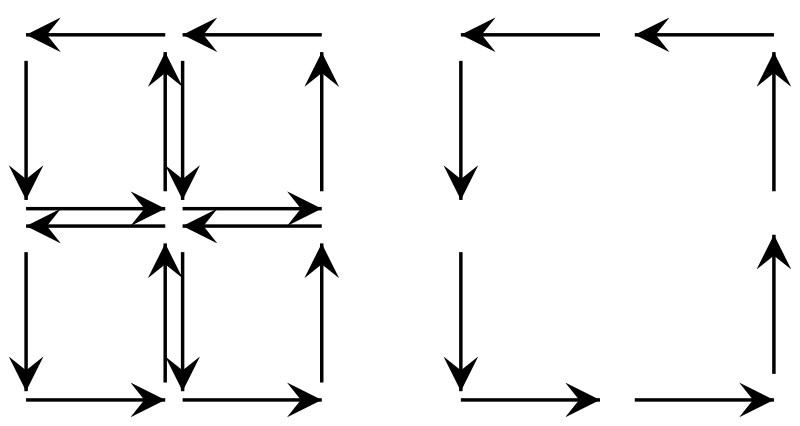
\includegraphics[width=.55\linewidth]{figures/N-20240427/stokes-patch.png}
\caption{A small oriented patch: the boundary orientation is part of the theorem.}
\end{figure}

\section{Stokes' theorem}

The central theorem is
\[
  \int_M d\omega=\int_{\partial M}\omega.
\]
This is Stokes' theorem. It says that the integral of a derivative over a region is controlled by the original quantity on the boundary.

Many familiar theorems are shadows of this one:
\[
\begin{array}{c|c}
\text{classical theorem} & \text{form-theoretic statement}\\
\hline
\text{Fundamental theorem of calculus} & \int_{[a,b]}df=f(b)-f(a)\\
\text{Green's theorem} & \int_D d(P\,dx+Q\,dy)=\int_{\partial D}P\,dx+Q\,dy\\
\text{Divergence theorem} & \int_M d\omega=\int_{\partial M}\omega
\end{array}
\]


% line integrals expanded example
\section{A worked example: line integrals}

Let
\[
  \omega=P(x,y)\,dx+Q(x,y)\,dy
\]
and let \(\gamma(t)=(x(t),y(t))\), \(a\le t\le b\). Pulling back \(\omega\) to the interval gives
\[
  \gamma^*\omega=\left(P(x(t),y(t))x'(t)+Q(x(t),y(t))y'(t)\right)dt.
\]
Thus
\[
  \int_\gamma \omega
  =\int_a^b
  \left(P(x(t),y(t))x'(t)+Q(x(t),y(t))y'(t)\right)dt.
\]
This is the usual line integral, but now it is explained by one operation: pull back the form to the parameter domain and integrate there.

\section{A worked example: Green's theorem}

For \(\omega=P\,dx+Q\,dy\),
\[
  d\omega=\left(\frac{\partial Q}{\partial x}-\frac{\partial P}{\partial y}\right)dx\wedge dy.
\]
Stokes' theorem on a planar region \(D\) says
\[
  \int_D d\omega=\int_{\partial D}\omega.
\]
In coordinates this becomes
\[
  \iint_D\left(\frac{\partial Q}{\partial x}-\frac{\partial P}{\partial y}\right)dx\,dy
  =\int_{\partial D}P\,dx+Q\,dy.
\]
So Green's theorem is not a separate miracle. It is Stokes' theorem written in two-dimensional coordinates.

\section{Why arc length is different}

A common confusion is to treat \(ds\) like a \(1\)-form. But arc length is not linear in the velocity:
\[
  ds(\gamma')=\|\gamma'\|dt.
\]
The norm is not a linear functional. Differential forms measure oriented quantities; metrics measure lengths and angles. Both are geometric, but they are not the same kind of structure.

\section{Why this viewpoint is worth learning}

Vector calculus has several different-looking integral theorems. Differential forms reveal one pattern behind them. Derivatives become exterior derivatives. Change of variables becomes pullback. Boundary signs become orientation. Integrals become pairings of forms with domains.

The slogan is:
\[
  \text{Stokes says that local change becomes boundary measurement.}
\]

\notechapter{N-20260403}{Double Integrals: Riemann Definition, Properties, Symmetry, and Mean Value}


\section{Definition}

Let $f$ be a bounded function on a bounded closed region $D\subseteq\mathbb R^2$.  Partition $D$ into small subregions $\Delta\sigma_i$, choose sample points $(\xi_i,\eta_i)$, and form
\[
  \sum_{i=1}^n f(\xi_i,\eta_i)\Delta\sigma_i.
\]
If this sum has a limit independent of the partition and sample points as the mesh tends to zero, the limit is the double integral
\[
  \iint_D f(x,y)\,d\sigma.
\]

\section{Basic properties}

Double integrals are linear, additive over regions, monotone, and compatible with estimates:
\[
  m\le f\le M\quad\Rightarrow\quad
  m\,\operatorname{area}(D)\le\iint_D f\,dA\le M\,\operatorname{area}(D).
\]
If $f$ is continuous on $D$, it is Riemann integrable.

\section{Symmetry}

If $D$ is symmetric and $f$ is odd with respect to that symmetry, then the integral is zero.  If $f$ is even, the integral over the full region is twice the integral over one half.  Symmetry is not a shortcut after computation; it is often the computation.

\section{Mean value theorem}

If $f$ is continuous on a connected bounded closed region $D$, then there exists $P_0\in D$ such that
\[
  \iint_D f\,dA=f(P_0)\operatorname{area}(D).
\]
This says that an integral is an average value multiplied by area.


\section{Meaning of the double-integral notation}

The annotated source image is better represented as notation rather than as a screenshot.  In
\[
  \iint_D f(x,y)\,d\sigma
  =\lim_{\lambda\to0}\sum_{i=1}^n f(\xi_i,\eta_i)\Delta\sigma_i,
\]
Here \(D\) is the integration region, \(f(x,y)\) is the integrand, and \(d\sigma\) is the area element.  The term \(f(\xi_i,\eta_i)\Delta\sigma_i\) is the contribution of one small cell in a Riemann sum.  The limit says that the mesh size \(\lambda\) tends to zero.

\section{Expanded synthesis and advanced context}

A double integral is the continuous version of adding weighted area elements.  Its most important conceptual move is to separate the integrand from the measure of the region.



\paragraph{Expanded synthesis.}
For this chapter, the elementary material should be read as a study of what remains invariant when coordinates change. The earlier sections (`Definition`, `Basic properties`, `Symmetry`, `Mean value theorem`) compute with arrays, bases, pivots, determinants, or eigenvectors; the deeper object is a linear map together with the spaces it acts on. A matrix is a representation of that map after bases have been chosen. This is why formulas such as
\[
  A' = P^{-1}AP,\qquad \widetilde A = T^{-1}AS
\]
are not cosmetic: they distinguish an intrinsic morphism from a coordinate description.

The structural hierarchy is as follows. Kernels record what a map forgets, images record what it reaches, cokernels record obstructions to solvability, and quotients record information after an equivalence has been imposed. Determinants act on the top exterior power and therefore measure oriented volume; traces are invariant under cyclic rearrangement and become characters in representation theory; adjoints depend on an inner product and lead to self-adjoint spectral theory.

A useful way to return to the computations is to ask, for every formula, which invariant it is measuring. Row reduction measures rank and kernel; diagonalization measures decomposition into invariant subspaces; Gram--Schmidt measures orthogonal projection; positive definiteness measures ellipsoid geometry; tensor notation measures how components transform. The elementary methods are therefore the finite-dimensional laboratory in which duality, quotienting, functoriality, and spectral decomposition can be seen clearly.


\section{Expanded Riemann-sum interpretation}

The Riemann definition says: divide a region into tiny pieces, multiply each tiny area by a sample value of the function, and let the largest diameter of the pieces go to zero.  The insistence on arbitrary partitions is important.  It ensures that the value of the integral belongs to the function and the region, not to a preferred grid.

When $f\ge0$, the double integral is volume under the surface $z=f(x,y)$.  When $f$ changes sign, it is signed volume.  When $f$ is a density, the integral is mass.

\section{Comparison examples}

If $D$ is symmetric about the $y$-axis and $f(x,y)=xg(x^2,y)$, then the integral is zero by oddness in $x$.  If $f$ is even with respect to that symmetry, the full integral is twice the integral over one half.  This is the kind of observation that should be made before computation.

\section{Mean value as average}

The formula
\[
  \iint_D f\,dA=f(\xi,\eta)\operatorname{area}(D)
\]
for continuous $f$ on connected compact $D$ says that the average value of $f$ is achieved somewhere.  It is the two-dimensional analogue of the one-variable integral mean value theorem.

\section{Elementary-to-advanced bridge: double integrals as measure integrals}

A double integral over a plane region $D$ is an integral with respect to two-dimensional Lebesgue measure:
\[
  \iint_D f(x,y)\,dA=\int_{\mathbb R^2} f(x,y)\mathbf 1_D(x,y)\,d\lambda^2.
\]
This point of view separates the function from the region.  The domain is represented by a characteristic function, and the area element is the underlying measure.

Tonelli's theorem says that for nonnegative measurable $f$,
\[
  \iint f\,d(\mu\times\nu)=\int\left(\int f(x,y)\,d\nu(y)\right)d\mu(x)
\]
without needing prior integrability.  Fubini's theorem gives the same iterated formula for integrable functions.

\section{Elementary-to-advanced bridge: product measures}

The reason iterated integrals work is product measure.  If $(X,\mu)$ and $(Y,\nu)$ are measure spaces, their product has measure $\mu\times\nu$ satisfying
\[
  (\mu\times\nu)(A\times B)=\mu(A)\nu(B).
\]
Rectangles generate the product sigma-algebra.  General regions are built from rectangles by limiting processes.

Thus the elementary partition of a plane region into small rectangles is the Riemann-sum shadow of product measure.

\section{Elementary-to-advanced bridge: change of variables theorem}

For a $C^1$ diffeomorphism $T:U\to V$,
\[
  \int_V f(x)\,dx=\int_U f(T(u))|\det DT(u)|\,du.
\]
The Jacobian determinant is the local area scaling.  The elementary polar-coordinate formula $dA=r\,dr\,d\theta$ is one instance.

The theorem is not merely computational: it says integration is compatible with smooth coordinate change, provided one accounts for local volume distortion.

\section{Returning to the double-integral examples}

The original Riemann-sum definition, region splitting, symmetry, and mean-value exercises are all preserved.  The advanced layer says that they belong to measure theory: double integrals use product measure, Fubini/Tonelli justify iterated integration, and change of variables is measure transformation under a differentiable map.

% Second-pass deepening for waves 2-4: wave 4 part 2
\section{Second-pass deepening: Fubini failures and why hypotheses matter}

For nonnegative functions, Tonelli's theorem allows iterated integration even if the integral is infinite.  For sign-changing functions, Fubini requires integrability of $|f|$.  Without that hypothesis, changing order may change the answer or make one order meaningless.

This matters because elementary calculus often trains order-switching as a geometric skill, but advanced analysis adds a convergence condition.  The region must be described correctly, and the function must be integrable in the appropriate sense.

\section{Second-pass deepening: symmetry as group action on measure}

If a region $D$ is invariant under a transformation $g$ and the measure is preserved, then
\[
  \int_D f\,dA=\int_D f\circ g\,dA.
\]
If $f\circ g=-f$, the integral is zero.  This is the group-action explanation of odd-function cancellation over symmetric domains.

The elementary symmetry shortcuts are therefore rigorous consequences of measure-preserving transformations.

\notechapter{N-20260405}{Computing Double Integrals: Fubini, Polar Coordinates, and Change of Variables}


\section{Iterated integrals}

If a plane region is vertically simple,
\[
  D=\{(x,y):a\le x\le b,\ \varphi_1(x)\le y\le \varphi_2(x)\},
\]
then Fubini's theorem gives
\[
  \iint_D f(x,y)\,dA=
  \int_a^b\int_{\varphi_1(x)}^{\varphi_2(x)}f(x,y)\,dy\,dx.
\]
If the region is horizontally simple, reverse the order.  The main work is not integrating; it is describing $D$ correctly.

\section{Changing the order}

Changing order means re-describing the same region with the other variable outermost.  A reliable method is: draw the projection interval, write lower and upper bounds, and split the region if a single formula cannot describe it.

\section{Polar coordinates}

For rotational or radial regions,
\[
  x=r\cos\theta,\qquad y=r\sin\theta,\qquad dA=r\,dr\,d\theta.
\]
The factor $r$ is the Jacobian.  It is the area scaling of the map $(r,\theta)\mapsto(x,y)$.

\section{General change of variables}

For a $C^1$ one-to-one transformation
\[
  x=x(u,v),\qquad y=y(u,v),
\]
the formula is
\[
  \iint_D f(x,y)\,dx\,dy=
  \iint_{D'} f(x(u,v),y(u,v))
  \left|\frac{\partial(x,y)}{\partial(u,v)}\right|\,du\,dv.
\]
The determinant is the local area multiplier.  This is the conceptual reason every coordinate transformation carries a Jacobian.

\section{The conceptual payoff}

Double-integral computation is a problem of choosing coordinates that make the region and integrand simple at the same time.  Fubini slices the region; polar coordinates exploit rotation; general change of variables is local linearization of area.



\paragraph{Expanded synthesis.}
For this chapter, the elementary material should be read as a study of what remains invariant when coordinates change. The earlier sections (`Iterated integrals`, `Changing the order`, `Polar coordinates`, `General change of variables`, `Higher viewpoint`) compute with arrays, bases, pivots, determinants, or eigenvectors; the deeper object is a linear map together with the spaces it acts on. A matrix is a representation of that map after bases have been chosen. This is why formulas such as
\[
  A' = P^{-1}AP,\qquad \widetilde A = T^{-1}AS
\]
are not cosmetic: they distinguish an intrinsic morphism from a coordinate description.

The structural hierarchy is as follows. Kernels record what a map forgets, images record what it reaches, cokernels record obstructions to solvability, and quotients record information after an equivalence has been imposed. Determinants act on the top exterior power and therefore measure oriented volume; traces are invariant under cyclic rearrangement and become characters in representation theory; adjoints depend on an inner product and lead to self-adjoint spectral theory.

A useful way to return to the computations is to ask, for every formula, which invariant it is measuring. Row reduction measures rank and kernel; diagonalization measures decomposition into invariant subspaces; Gram--Schmidt measures orthogonal projection; positive definiteness measures ellipsoid geometry; tensor notation measures how components transform. The elementary methods are therefore the finite-dimensional laboratory in which duality, quotienting, functoriality, and spectral decomposition can be seen clearly.


\section{Expanded order-changing method}

To change an integral order, never start by manipulating symbols.  Start from the region.  For example, if
\[
  0\le x\le1,\qquad x^2\le y\le x,
\]
then the projection on the $y$-axis is $0\le y\le1$, and the horizontal slice satisfies
\[
  y\le x\le \sqrt y.
\]
Thus
\[
  \int_0^1\int_{x^2}^{x}f(x,y)\,dy\,dx
  =
  \int_0^1\int_y^{\sqrt y}f(x,y)\,dx\,dy.
\]
The method is always geometric: inequalities must be solved as a description of the same set.

\section{Jacobian as local area determinant}

For $T(u,v)=(x(u,v),y(u,v))$, the derivative matrix
\[
  DT=\begin{pmatrix}x_u&x_v\\y_u&y_v\end{pmatrix}
\]
sends a tiny $du\,dv$ rectangle to an approximate parallelogram.  Its area is multiplied by $|\det DT|$.  This is why the absolute value of the Jacobian appears in change of variables.

\section{Jacobian as determinant of a pullback}

For a coordinate change
\[
  x=x(u,v),\qquad y=y(u,v),
\]
the differential forms transform as
\[
  dx=x_u\,du+x_v\,dv,\qquad dy=y_u\,du+y_v\,dv.
\]
Taking the wedge product gives
\[
  dx\wedge dy=(x_uy_v-x_vy_u)\,du\wedge dv.
\]
Thus
\[
  dx\wedge dy=\det\frac{\partial(x,y)}{\partial(u,v)}\,du\wedge dv.
\]
The Jacobian is the coefficient by which the coordinate change pulls back the area form.

This is the differential-form version of the elementary change-of-variables formula.

\section{Coarea formula preview}

Changing variables is one way to decompose integration.  The coarea formula is a more advanced generalization.  For a smooth map $F:\mathbb R^n\to\mathbb R^k$, it relates an integral over the domain to integrals over level sets of $F$:
\[
  \int_{\mathbb R^n} g(x)J_F(x)\,dx
  =\int_{\mathbb R^k}\left(\int_{F^{-1}(y)} g\,d\mathcal H^{n-k}\right)dy.
\]
For $k=1$, this decomposes volume by level surfaces.

The elementary method of slicing a region vertically or horizontally is a simple coarea idea: integrate first over fibers, then over the parameter indexing the fibers.

\section{Orientation and absolute value}

In ordinary area integrals, the absolute value of the Jacobian appears:
\[
  dA=|J|\,du\,dv.
\]
For oriented forms, the sign is retained:
\[
  dx\wedge dy=J\,du\wedge dv.
\]
This distinction explains why flux integrals and Green/Stokes formulas care about orientation, while scalar area integrals do not.

\section{Returning to order changes}

Changing integration order is not a syntactic operation on bounds; it is a choice of projection and fibers.  General change of variables replaces rectangular fibers by smooth coordinate fibers.  The original exercises teach the finite-dimensional geometry needed for the more general integration theorems.

% Second-pass deepening for waves 2-4: wave 4 part 2
\section{Change of variables as local linearization}

At a point $u$, the differentiable map $T$ is approximated by its derivative
\[
  T(u+h)=T(u)+DT(u)h+o(|h|).
\]
Small squares in parameter space become approximate parallelograms in physical space.  The determinant $\det DT(u)$ measures their oriented area scaling.

This is why the Jacobian appears locally and is then integrated globally.  The change-of-variables theorem is the accumulation of infinitely many local linear approximations.

\section{Singular coordinate systems}

Polar coordinates fail to be one-to-one at the origin and are periodic in $\theta$.  Spherical coordinates have singularities at the poles.  These singularities usually do not harm integrals because they occur on sets of measure zero, but they matter for topology and vector fields.

This explains why coordinate formulas must be used with awareness of domains.  A coordinate system may be excellent for integration but poor for global topology.

\notechapter{N-20260406}{Triple Integrals: Rectangular, Cylindrical, and Spherical Coordinates}


\section{Definition and Fubini principle}

A triple integral accumulates a scalar field over a spatial region $\Omega\subseteq\mathbb R^3$:
\[
  \iiint_\Omega f(x,y,z)\,dV.
\]
For a box or simple region, it becomes an iterated integral.  A typical $xy$-simple region has
\[
  (x,y)\in D,\qquad z_1(x,y)\le z\le z_2(x,y),
\]
so
\[
  \iiint_\Omega f\,dV=\iint_D\int_{z_1}^{z_2}f(x,y,z)\,dz\,dA.
\]

\section{Cylindrical coordinates}

Cylindrical coordinates are
\[
  x=r\cos\theta,\quad y=r\sin\theta,\quad z=z,\quad dV=r\,dr\,d\theta\,dz.
\]
They are natural for cylinders, cones, and solids with axial symmetry.

\section{Spherical coordinates}

With
\[
  x=\rho\sin\varphi\cos\theta,\quad
  y=\rho\sin\varphi\sin\theta,\quad
  z=\rho\cos\varphi,
\]
one has
\[
  dV=\rho^2\sin\varphi\,d\rho\,d\varphi\,d\theta.
\]
The factor comes from the small lengths $d\rho$, $\rho d\varphi$, and $\rho\sin\varphi d\theta$.

\section{Applications}

Mass, center of mass, and moments are all integrals of density multiplied by coordinate functions.  For density $\rho(x,y,z)$,
\[
  M=\iiint_\Omega \rho\,dV,\qquad
  \bar x=\frac1M\iiint_\Omega x\rho\,dV.
\]

\section{Looking ahead}

A triple integral is a measure of volume weighted by a function.  The coordinate system should be chosen so that the boundary of the region becomes simple and the Jacobian expresses the local volume scaling.



\paragraph{Expanded synthesis.}
The common theme of this chapter is that a limiting or computational rule becomes powerful only after one specifies the space in which the limit takes place. The earlier sections on Fubini's principle, cylindrical coordinates, spherical coordinates, applications, and the higher viewpoint may look separate. They ask the same question: which operations are stable under approximation? A derivative is stable first-order approximation,
\[
  f(a+h)=f(a)+L(h)+o(|h|),
\]
while an integral is stable accumulation with respect to a measure, and a convergent series is a limit in a chosen norm or topology.

The advanced bridge is functional-analytic. Uniform convergence is convergence in a sup norm; $L^p$ convergence is convergence in an integral norm; differentiability is the existence of a continuous linear approximation; many differential equations are operator equations $L[u]=f$. Theorems such as dominated convergence, the inverse function theorem, the projection theorem in Hilbert spaces, and semigroup existence results are refined answers to the same elementary concern: when may we pass from finite approximations to a genuine limiting object?

To use this viewpoint when rereading the original examples, identify the hidden stability condition. A Taylor expansion asks for control of the remainder. A change of variables asks for differentiability and Jacobian control. Termwise differentiation of a series asks for uniform convergence of derivative series. A differential-equation formula asks whether the operator is invertible under the imposed initial or boundary data. The elementary computation is the visible part; the advanced theory names the hypotheses that make it legitimate.


\section{Expanded coordinate-choice strategy}

Rectangular coordinates are good when the region is bounded by coordinate planes or graphs over coordinate planes.  Cylindrical coordinates are good when $x^2+y^2$ appears or the region has rotational symmetry about the $z$-axis.  Spherical coordinates are good when $x^2+y^2+z^2$ or cones from the origin appear.

The mistake to avoid is using a beautiful coordinate system for the integrand but a terrible one for the boundary.  The best coordinates simplify both the integrand and the region.

\section{Symmetry in triple integrals}

If $\Omega$ is symmetric about $x=0$ and the integrand is odd in $x$, then
\[
  \iiint_\Omega f(x,y,z)\,dV=0.
\]
If the integrand is even in $x$, the integral over $\Omega$ is twice the integral over the half-region $x\ge0$.  In three dimensions, symmetry can remove entire coordinates from computation.

\section{Volume forms}

In $\mathbb R^3$, the standard volume form is
\[
  dx\wedge dy\wedge dz.
\]
A coordinate change $(u,v,w)\mapsto(x,y,z)$ pulls it back to
\[
  dx\wedge dy\wedge dz
  =\det\frac{\partial(x,y,z)}{\partial(u,v,w)}\,du\wedge dv\wedge dw.
\]
This is the differential-form explanation of the Jacobian in triple integrals.

For cylindrical coordinates,
\[
  dV=r\,dr\,d\theta\,dz.
\]
For spherical coordinates,
\[
  dV=\rho^2\sin\varphi\,d\rho\,d\varphi\,d\theta.
\]
These factors are not mnemonics; they are determinants of coordinate maps.

\section{Divergence theorem preparation}

Triple integrals of divergence appear in Gauss' theorem:
\[
  \iiint_\Omega \nabla\cdot F\,dV=\iint_{\partial\Omega}F\cdot n\,dS.
\]
Before one learns the theorem, triple integrals train the measurement of total source over a volume.  After the theorem, the same integral becomes a boundary flux.

The elementary density interpretation also fits: if $\rho(x,y,z)$ is mass density, then
\[
  M=\iiint_\Omega \rho\,dV.
\]
If $\nabla\cdot F$ is source density, the same integral is total production inside $\Omega$.

\section{Measure-preserving transformations}

A transformation is volume-preserving if
\[
  |\det DT|=1.
\]
Rotations and translations preserve volume.  Hamiltonian flows in phase space preserve symplectic volume by Liouville's theorem.

Thus the elementary Jacobian test connects to dynamics: some transformations move regions around without changing volume.  This is important in mechanics, ergodic theory, and PDE transport equations.

\section{Returning to coordinate systems}

Rectangular, cylindrical, and spherical coordinates should be chosen not by habit but by symmetry.  The advanced viewpoint says: choose coordinates adapted to the geometry, compute the pulled-back volume form, then integrate over the parameter domain.

% Second-pass deepening for waves 2-4: wave 4 part 2
\section{Volume, density, and pushforward}

If $T:U\to V$ is a coordinate map, then a density on $V$ pulls back to a density on $U$ by multiplying with $|\det DT|$.  Conversely, one may push forward a density through $T$.  In probability, this is the change-of-variables formula for random variables.

For example, if a random vector has density $f_X(x)$ and $Y=T(X)$ with invertible $T$, then
\[
  f_Y(y)=f_X(T^{-1}y)|\det DT^{-1}(y)|.
\]
Triple-integral Jacobians are therefore the same mathematics as probability density transformations.

\section{Divergence and infinitesimal volume change}

If a vector field $F$ generates a flow $\Phi_t$, then divergence measures infinitesimal volume expansion:
\[
  \frac d{dt}\bigg|_{t=0}\operatorname{vol}(\Phi_t(\Omega))=\int_\Omega \nabla\cdot F\,dV.
\]
Thus the divergence theorem relates local infinitesimal expansion to flux through the boundary.

The elementary triple integral of $\nabla\cdot F$ is therefore measuring total infinitesimal source over a region.

\notechapter{N-20260408}{Volumes, Spatial Regions, and Order of Integration}


\section{Volume by double and triple integrals}

If a curved cylinder has top $z=f(x,y)$ over a plane region $D$, then its volume is
\[
  V=\iint_D f(x,y)\,dx\,dy.
\]
For a solid region $\Omega$,
\[
  V=\iiint_\Omega 1\,dV.
\]
These formulas are the same idea: integrate a density of $1$ over the appropriate measure.

\section{Describing spatial regions}

A region may be $xy$-simple, $yz$-simple, or $zx$-simple.  For example,
\[
  \Omega=\{(x,y,z):(x,y)\in D,\ z_1(x,y)\le z\le z_2(x,y)\}.
\]
If a single description is impossible, split the region.  Most difficult triple-integral problems are difficult because of the geometry of $\Omega$, not because of the antiderivatives.

\begin{figure}[H]
\centering
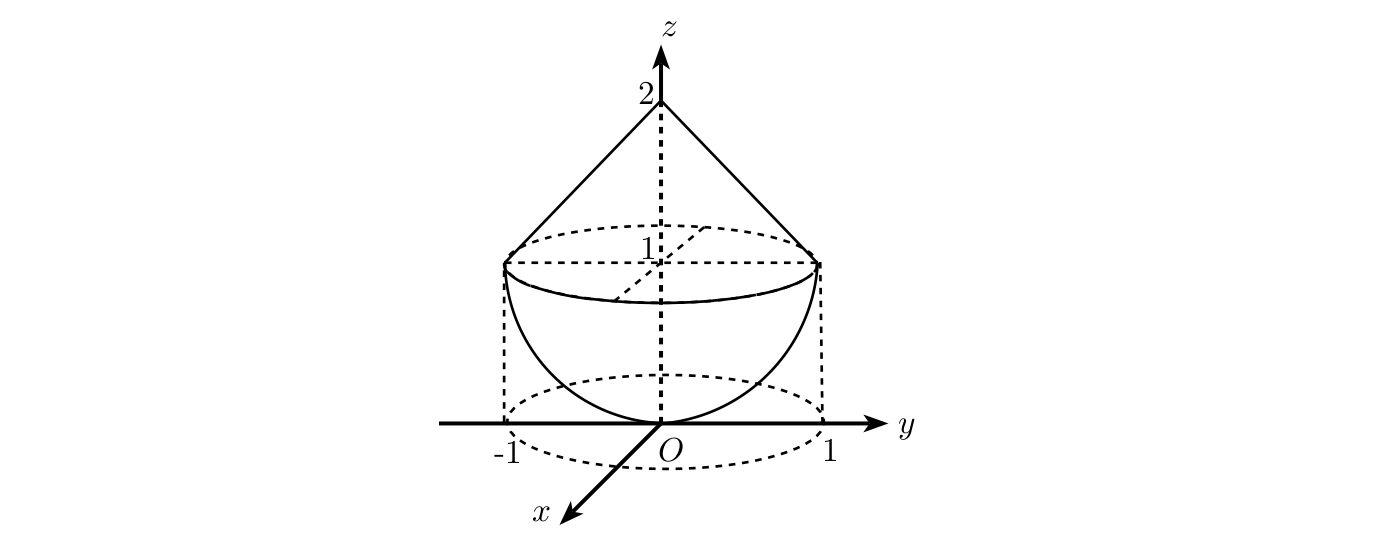
\includegraphics[width=0.78\textwidth,height=0.74\textheight,keepaspectratio]{figures/notes-md/N-20260408/N-20260408-fig-01-composite-solid-hemisphere-and-cone.png}
\caption{A composite solid with a hemispherical part and a conical part.  The picture is used to decide cross-sections and height bounds before writing the integral.}
\end{figure}


\section{Changing order of integration}

Changing the order means projecting the region onto a different coordinate plane and rewriting the boundary.  The safe procedure is: identify the shadow, determine the inner variable's lower and upper surfaces, and split the shadow if necessary.




\begin{figure}[H]
\centering
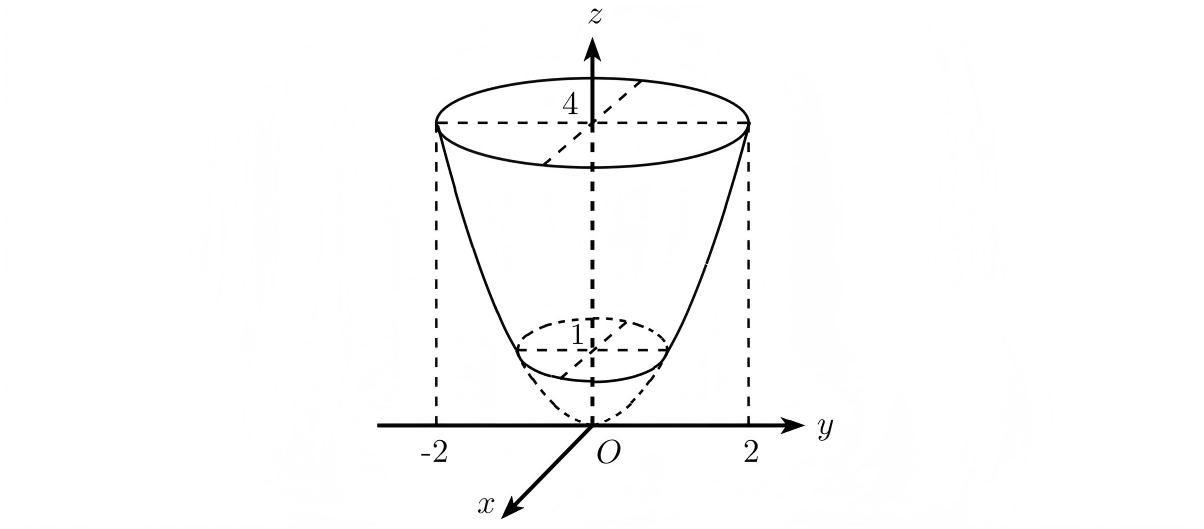
\includegraphics[width=0.78\textwidth,height=0.74\textheight,keepaspectratio]{figures/notes-md/N-20260408/N-20260408-fig-02-truncated-rotational-solid.png}
\caption{A rotational solid with circular cross-sections at different heights.  Such diagrams are read by projecting to the base plane and then recovering the vertical bounds.}
\end{figure}

\section{Expanded synthesis and advanced context}

Integration over regions is geometric bookkeeping.  The same solid can be sliced in many directions, and the best order is the one that makes both the limits and the integrand transparent.



\paragraph{Expanded synthesis.}
For this chapter, the elementary material should be read as a study of what remains invariant when coordinates change. The earlier sections (`Volume by double and triple integrals`, `Describing spatial regions`, `Changing order of integration`, `Higher viewpoint`) compute with arrays, bases, pivots, determinants, or eigenvectors; the deeper object is a linear map together with the spaces it acts on. A matrix is a representation of that map after bases have been chosen. This is why formulas such as
\[
  A' = P^{-1}AP,\qquad \widetilde A = T^{-1}AS
\]
are not cosmetic: they distinguish an intrinsic morphism from a coordinate description.

The structural hierarchy is as follows. Kernels record what a map forgets, images record what it reaches, cokernels record obstructions to solvability, and quotients record information after an equivalence has been imposed. Determinants act on the top exterior power and therefore measure oriented volume; traces are invariant under cyclic rearrangement and become characters in representation theory; adjoints depend on an inner product and lead to self-adjoint spectral theory.

A useful way to return to the computations is to ask, for every formula, which invariant it is measuring. Row reduction measures rank and kernel; diagonalization measures decomposition into invariant subspaces; Gram--Schmidt measures orthogonal projection; positive definiteness measures ellipsoid geometry; tensor notation measures how components transform. The elementary methods are therefore the finite-dimensional laboratory in which duality, quotienting, functoriality, and spectral decomposition can be seen clearly.


\section{Expanded region reconstruction}

Spatial-integration examples usually fail at the same point: the student sees the integral but not the solid.  A good reconstruction process is:

\begin{enumerate}[(i)]
  \item identify the surfaces that bound the solid;
  \item draw or mentally project the solid onto a coordinate plane;
  \item decide which variable has the simplest lower and upper bounds;
  \item split the region only when a single set of bounds would hide a boundary change.
\end{enumerate}

For a solid between $z=z_1(x,y)$ and $z=z_2(x,y)$ above $D$, the volume is
\[
  V=\iint_D [z_2(x,y)-z_1(x,y)]\,dA.
\]
This is the double-integral version of ``top minus bottom.''

\section{Why pictures remain useful}

\notechapter{N-20260416}{Line Integrals and Surface Integrals of the First and Second Kind}


\section{Line integrals with respect to arc length}

For a smooth curve $C:r(t)=(x(t),y(t))$, $a\le t\le b$, the first-kind line integral is
\[
  \int_C f(x,y)\,ds=\int_a^b f(x(t),y(t))\sqrt{x'(t)^2+y'(t)^2}\,dt.
\]
It integrates scalar density along length.

\section{Line integrals of vector fields}

For a vector field $F=(P,Q)$,
\[
  \int_C P\,dx+Q\,dy=\int_a^b [P(x(t),y(t))x'(t)+Q(x(t),y(t))y'(t)]\,dt.
\]
This is work or circulation.  Orientation matters.

\section{Surface integrals}

For a parametrized surface $r(u,v)$,
\[
  dS=\|r_u\times r_v\|\,du\,dv.
\]
The first-kind surface integral is
\[
  \iint_S f\,dS=\iint_D f(r(u,v))\|r_u\times r_v\|\,du\,dv.
\]
For a vector field $F$, the flux integral is
\[
  \iint_S F\cdot n\,dS=\iint_D F(r(u,v))\cdot(r_u\times r_v)\,du\,dv,
\]
with sign determined by orientation.

\section{Expanded synthesis and advanced context}

First-kind integrals integrate scalar density against geometric measure; second-kind integrals integrate vector fields through oriented curves or surfaces.  The difference is density versus flux.



\paragraph{Expanded synthesis.}
For this chapter, the elementary material should be read as a study of what remains invariant when coordinates change. The earlier sections (`Line integrals with respect to arc length`, `Line integrals of vector fields`, `Surface integrals`, `Higher viewpoint`, `Expanded distinction between first and second kind`) compute with arrays, bases, pivots, determinants, or eigenvectors; the deeper object is a linear map together with the spaces it acts on. A matrix is a representation of that map after bases have been chosen. This is why formulas such as
\[
  A' = P^{-1}AP,\qquad \widetilde A = T^{-1}AS
\]
are not cosmetic: they distinguish an intrinsic morphism from a coordinate description.

The structural hierarchy is as follows. Kernels record what a map forgets, images record what it reaches, cokernels record obstructions to solvability, and quotients record information after an equivalence has been imposed. Determinants act on the top exterior power and therefore measure oriented volume; traces are invariant under cyclic rearrangement and become characters in representation theory; adjoints depend on an inner product and lead to self-adjoint spectral theory.

A useful way to return to the computations is to ask, for every formula, which invariant it is measuring. Row reduction measures rank and kernel; diagonalization measures decomposition into invariant subspaces; Gram--Schmidt measures orthogonal projection; positive definiteness measures ellipsoid geometry; tensor notation measures how components transform. The elementary methods are therefore the finite-dimensional laboratory in which duality, quotienting, functoriality, and spectral decomposition can be seen clearly.


\section{Expanded distinction between first and second kind}

For line integrals, the first kind
\[
  \int_C f\,ds
\]
does not depend on orientation.  Reversing the parametrization leaves $ds$ unchanged.  The second kind
\[
  \int_C P\,dx+Q\,dy
\]
does depend on orientation, because $dx$ and $dy$ change sign.

For surface integrals, the same distinction holds.  The scalar surface integral $\iint_S f\,dS$ has no orientation.  The flux integral $\iint_SF\cdot n\,dS$ requires a choice of normal and changes sign when the normal is reversed.

\section{Parametric formulas as one template}

For curves, the geometric element is $|r'(t)|\,dt$.  For surfaces, it is $|r_u\times r_v|\,du\,dv$.  These are the same idea: the derivative of a parametrization tells how much the parameter domain is stretched into the actual geometric object.

\section{Elementary-to-advanced bridge: scalar integrals versus forms}

A first-kind line integral
\[
  \int_C f\,ds
\]
integrates a scalar density against arclength.  It depends on the metric because $ds$ is a length element.  A second-kind line integral
\[
  \int_C P\,dx+Q\,dy+R\,dz
\]
integrates a one-form.  It depends on orientation, not directly on arclength.

Similarly, a scalar surface integral
\[
  \iint_S f\,dS
\]
uses the metric area element, while a flux integral integrates a two-form or an oriented normal field.  This is why reversing orientation changes flux but not scalar area.

The elementary distinction between first and second kind is therefore the first encounter with the difference between metric measure and oriented differential forms.

\section{Elementary-to-advanced bridge: flux as a two-form}

For a vector field $F=(P,Q,R)$ in $\mathbb R^3$, the flux form is
\[
  \omega_F=P\,dy\wedge dz+Q\,dz\wedge dx+R\,dx\wedge dy.
\]
If $S$ is oriented, then
\[
  \iint_SF\cdot n\,dS=\iint_S \omega_F.
\]
The normal-vector formula is a Euclidean translation of this two-form integral.

This is more than notation.  Differential forms automatically encode orientation and pullback under parametrization.  If $r(u,v)$ parametrizes $S$, then
\[
  \iint_S\omega_F=\iint_D r^*\omega_F.
\]
The usual cross-product formula is the coordinate expression of this pullback.

\section{Elementary-to-advanced bridge: orientation bundles}

A surface may or may not admit a globally consistent normal direction.  Orientable surfaces, such as the sphere and torus, do.  The Möbius strip does not.  Flux integrals require an orientation, so they are globally well-defined only on oriented surfaces or after choosing local orientations carefully.

This explains why surface orientation is not a minor sign convention.  It is a topological property of the surface.

\section{Elementary-to-advanced bridge: manifolds with boundary}

A curve or surface used in integration is an example of a manifold.  A parametrized curve is a one-dimensional manifold; a surface is a two-dimensional manifold.  Boundaries appear naturally: a surface patch has boundary curves, and Stokes' theorem relates integration over the boundary to integration over the interior.

Thus the elementary parametrization formulas are local coordinate charts for manifolds.  The advanced language keeps the same computations but removes dependence on a single global parametrization.

% Second-pass deepening for waves 2-4: wave 4 part 2
\section{Second-pass deepening: parametrization invariance}

A well-defined geometric integral should not depend on the chosen parametrization.  For a first-kind line integral, reparametrizing $t=\phi(s)$ changes $|r'(t)|dt$ into $|(r\circ\phi)'(s)|ds$, so the value is unchanged for orientation-preserving reparametrizations.

For a one-form integral, orientation matters.  Reversing the parametrization changes sign.  This is exactly what should happen for work or circulation: traversing a path backward reverses the accumulated oriented effect.

\section{Second-pass deepening: surface normals as choices of orientation}

For a parametrized surface $r(u,v)$, the vector $r_u\times r_v$ depends on the order of parameters.  Swapping $u$ and $v$ reverses orientation.  The flux integral is therefore an integral over an oriented surface, not merely over a set of points.

The elementary cross-product normal formula is the coordinate expression of choosing an orientation on a two-dimensional manifold.

\notechapter{N-20260417}{Green Formula, Conservative Fields, and the Planar Stokes Principle}


\section{Green's theorem}

For a positively oriented simple closed curve $C=\partial D$ and sufficiently smooth $P,Q$,
\[
  \oint_C P\,dx+Q\,dy
  =\iint_D \left(\frac{\partial Q}{\partial x}-\frac{\partial P}{\partial y}\right)\,dA.
\]
The left side is circulation along the boundary; the right side is accumulated local rotation over the region.

\begin{figure}[H]
\centering
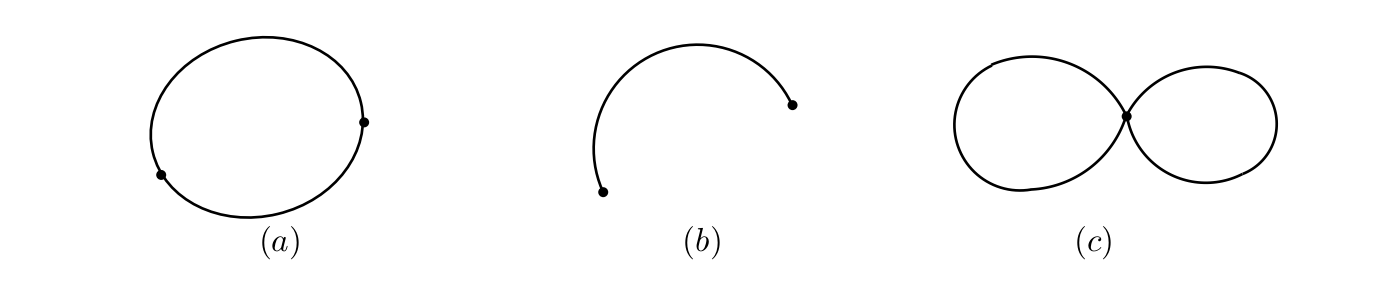
\includegraphics[width=0.82\textwidth,height=0.74\textheight,keepaspectratio]{figures/notes-md/N-20260417/N-20260417-fig-01-green-simple-closed-curves.png}
\caption{Simple closed curves and non-simple closed curves in the statement of Green's theorem.}
\end{figure}


\section{Path independence}

A vector field $F=(P,Q)$ is conservative if there exists $\phi$ such that
\[
  \nabla \phi=F.
\]
Then
\[
  \int_C P\,dx+Q\,dy=\phi(B)-\phi(A)
\]
for any path from $A$ to $B$.  On a simply connected region, $P_y=Q_x$ is the usual test for conservativity.

\begin{figure}[H]
\centering
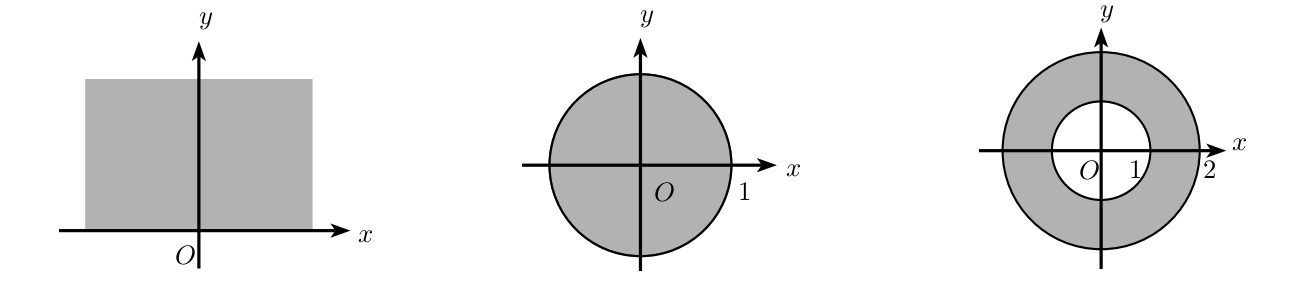
\includegraphics[width=0.82\textwidth,height=0.74\textheight,keepaspectratio]{figures/notes-md/N-20260417/N-20260417-fig-02-green-simply-connected-regions.png}
\caption{Simply connected and multiply connected plane regions.  The distinction matters for path independence and conservative fields.}
\end{figure}




\section{Expanded synthesis and advanced context}

Green's theorem is Stokes' theorem in the plane.  It says that the integral of a differential form over a boundary equals the integral of its derivative over the region.  This is the conceptual bridge to surface flux, Gauss' theorem, and the general Stokes theorem.



\paragraph{Expanded synthesis.}
For this chapter, the elementary material should be read as a study of what remains invariant when coordinates change. The earlier sections (`Green's theorem`, `Path independence`, `Higher viewpoint`, `Expanded Green-theorem proof idea`) compute with arrays, bases, pivots, determinants, or eigenvectors; the deeper object is a linear map together with the spaces it acts on. A matrix is a representation of that map after bases have been chosen. This is why formulas such as
\[
  A' = P^{-1}AP,\qquad \widetilde A = T^{-1}AS
\]
are not cosmetic: they distinguish an intrinsic morphism from a coordinate description.

The structural hierarchy is as follows. Kernels record what a map forgets, images record what it reaches, cokernels record obstructions to solvability, and quotients record information after an equivalence has been imposed. Determinants act on the top exterior power and therefore measure oriented volume; traces are invariant under cyclic rearrangement and become characters in representation theory; adjoints depend on an inner product and lead to self-adjoint spectral theory.

A useful way to return to the computations is to ask, for every formula, which invariant it is measuring. Row reduction measures rank and kernel; diagonalization measures decomposition into invariant subspaces; Gram--Schmidt measures orthogonal projection; positive definiteness measures ellipsoid geometry; tensor notation measures how components transform. The elementary methods are therefore the finite-dimensional laboratory in which duality, quotienting, functoriality, and spectral decomposition can be seen clearly.


\section{Expanded Green-theorem proof idea}

For a rectangle, Green's theorem can be checked by the fundamental theorem of calculus.  The $Q\,dy$ part accumulates horizontal changes in $Q$, and the $P\,dx$ part accumulates vertical changes in $P$ with the opposite sign.

Summing small rectangles makes interior boundary contributions cancel, leaving only the outer boundary.

This cancellation is the core of all Stokes-type theorems.  Local boundary pieces cancel in pairs; only the global boundary remains.

\begin{figure}[H]
\centering
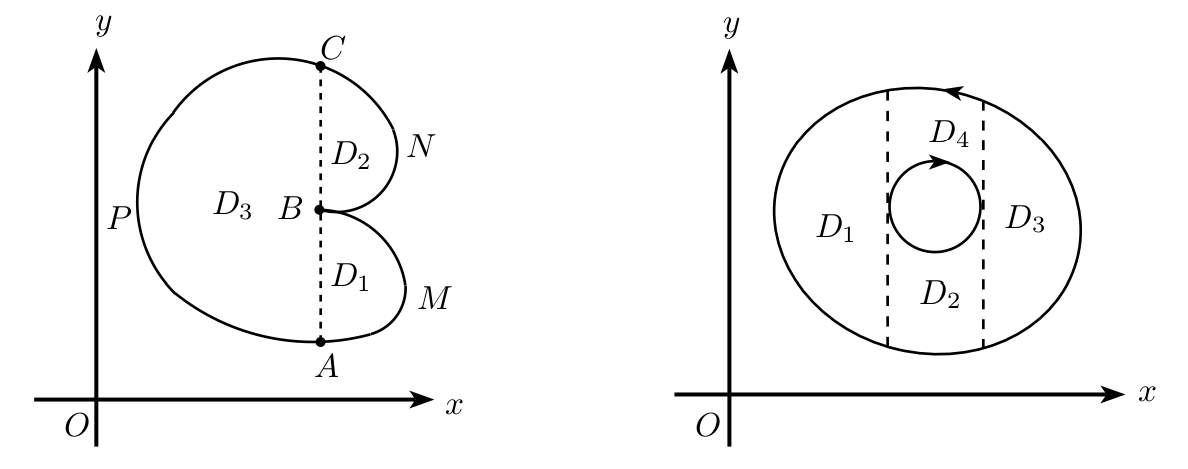
\includegraphics[width=0.82\textwidth,height=0.74\textheight,keepaspectratio]{figures/notes-md/N-20260417/N-20260417-fig-04-green-subdivision-boundary-cancellation.png}
\caption{Subdivision by auxiliary arcs: internal boundary contributions cancel, leaving only the outer boundary.}
\end{figure}


\section{Conservative fields and topology}

The condition $P_y=Q_x$ says that local curl is zero.  On a simply connected region, this implies the field is conservative.  On a region with a hole, it may fail.  The standard example is
\[
  F(x,y)=\left(-\frac{y}{x^2+y^2},\frac{x}{x^2+y^2}\right)
\]
on $\mathbb R^2\setminus\{0\}$.  Its curl is zero away from the origin, but circulation around the unit circle is $2\pi$.

\section{Elementary-to-advanced bridge: closed forms and exact forms}

For a plane vector field $F=(P,Q)$, the form
\[
  \omega=P\,dx+Q\,dy
\]
is closed when
\[
  d\omega=(Q_x-P_y)\,dx\wedge dy=0.
\]
It is exact when $\omega=df$ for some potential $f$.

Exact implies closed because $d^2=0$.  The converse depends on topology.  On simply connected domains in the plane, closed one-forms are exact.  On a punctured plane, this can fail.

\section{Elementary-to-advanced bridge: de Rham cohomology}

The first de Rham cohomology group is
\[
  H^1_{dR}(M)=\frac{\ker(d:\Omega^1(M)\to\Omega^2(M))}{\operatorname{im}(d:\Omega^0(M)\to\Omega^1(M))}.
\]
It measures closed one-forms modulo exact ones.  If $H^1_{dR}(M)=0$, every closed one-form is exact.

The standard form on the punctured plane,
\[
  \omega=\frac{-y\,dx+x\,dy}{x^2+y^2},
\]
is closed but not exact, because
\[
  \int_{S^1}\omega=2\pi.
\]
This integral detects the hole at the origin.

\section{Elementary-to-advanced bridge: Green's theorem as Stokes theorem}

Green's theorem says
\[
  \oint_{\partial D}P\,dx+Q\,dy
  =\iint_D (Q_x-P_y)\,dx\,dy.
\]
In differential-form notation, this is
\[
  \int_{\partial D}\omega=\int_D d\omega.
\]
This is exactly Stokes' theorem in dimension two.

The original path-independence tests therefore belong to a broad principle: boundary integrals measure the integral of a derivative over the interior.

\section{Elementary-to-advanced bridge: harmonic forms}

On a compact Riemannian manifold, each de Rham cohomology class has a unique harmonic representative.  A harmonic form satisfies
\[
  \Delta \omega=0,
\]
where $\Delta$ is the Hodge Laplacian.  This is Hodge theory.

For elementary vector calculus, the hint is this: fields can be decomposed into gradient-like, curl-like, and harmonic parts.  The harmonic part records topology.  This is the high-level continuation of conservative-field tests.

% Second-pass deepening for waves 2-4: wave 4 part 3
\section{Second-pass deepening: circulation as obstruction to a potential}

A field can have zero curl locally but still fail to have a global potential.  The punctured-plane form
\[
  \omega=\frac{-y\,dx+x\,dy}{x^2+y^2}
\]
is the standard example.  It is locally $d\theta$, but $\theta$ cannot be chosen as a single-valued global function on the punctured plane.

The integral
\[
  \int_{S^1}\omega=2\pi
\]
measures winding around the missing point.  Thus a line integral can detect topology.  This is the serious meaning behind the elementary warning that $P_y=Q_x$ is not enough on a domain with holes.

\section{Second-pass deepening: Green's theorem as cancellation of internal boundaries}

One way to understand Green's theorem is to subdivide a region into many small rectangles.  The boundary integrals over internal edges cancel because each internal edge is traversed twice in opposite directions.  Only the outer boundary remains.  This cancellation principle survives in chain complexes, singular homology, and general Stokes theorem.

The elementary proof by rectangles therefore already contains the algebraic identity
\[
  \partial^2=0,
\]
namely: the boundary of a boundary cancels.

\notechapter{N-20260615}{Surface Integrals, Gauss Theorem, and Stokes Theorem}

\section{Why this note is split this way}


\section{Four integrals that look similar but mean different things}

The first task is to separate four objects:
\[
  \iint_S f(x,y,z)\,dS,\qquad
  \iint_S P\,dy\,dz+Q\,dz\,dx+R\,dx\,dy,
\]
\[
  \iiint_\Omega \nabla\cdot F\,dV,\qquad
  \oint_{\partial S}P\,dx+Q\,dy+R\,dz.
\]
The first is a scalar surface integral: it integrates a scalar density over area.  The second is a flux integral: it integrates a vector field through an oriented surface.  The third is the volume integral of divergence.  The fourth is circulation along an oriented boundary curve.

The common mistake is to treat all of them as ``surface integral formulas.''  They are not the same mathematical object.  Their relation is supplied by Gauss' theorem and Stokes' theorem.

\section{First-kind surface integrals}

Let $S$ be a smooth surface parametrized by
\[
  r(u,v)=(x(u,v),y(u,v),z(u,v)),\qquad (u,v)\in D.
\]
Then
\[
  dS=|r_u\times r_v|\,du\,dv,\qquad
  \iint_S f\,dS=\iint_D f(r(u,v))|r_u\times r_v|\,du\,dv.
\]
This is the surface analogue of the first-kind line integral $\int_C f\,ds$.

For a graph $z=z(x,y)$,
\[
  r(x,y)=(x,y,z(x,y)),\qquad
  r_x\times r_y=(-z_x,-z_y,1),
\]
so
\[
  dS=\sqrt{1+z_x^2+z_y^2}\,dx\,dy.
\]
For a graph $x=x(y,z)$ or $y=y(z,x)$, analogous formulas hold:
\[
  dS=\sqrt{1+x_y^2+x_z^2}\,dy\,dz,\qquad
  dS=\sqrt{1+y_z^2+y_x^2}\,dz\,dx.
\]


\begin{figure}[H]
\centering
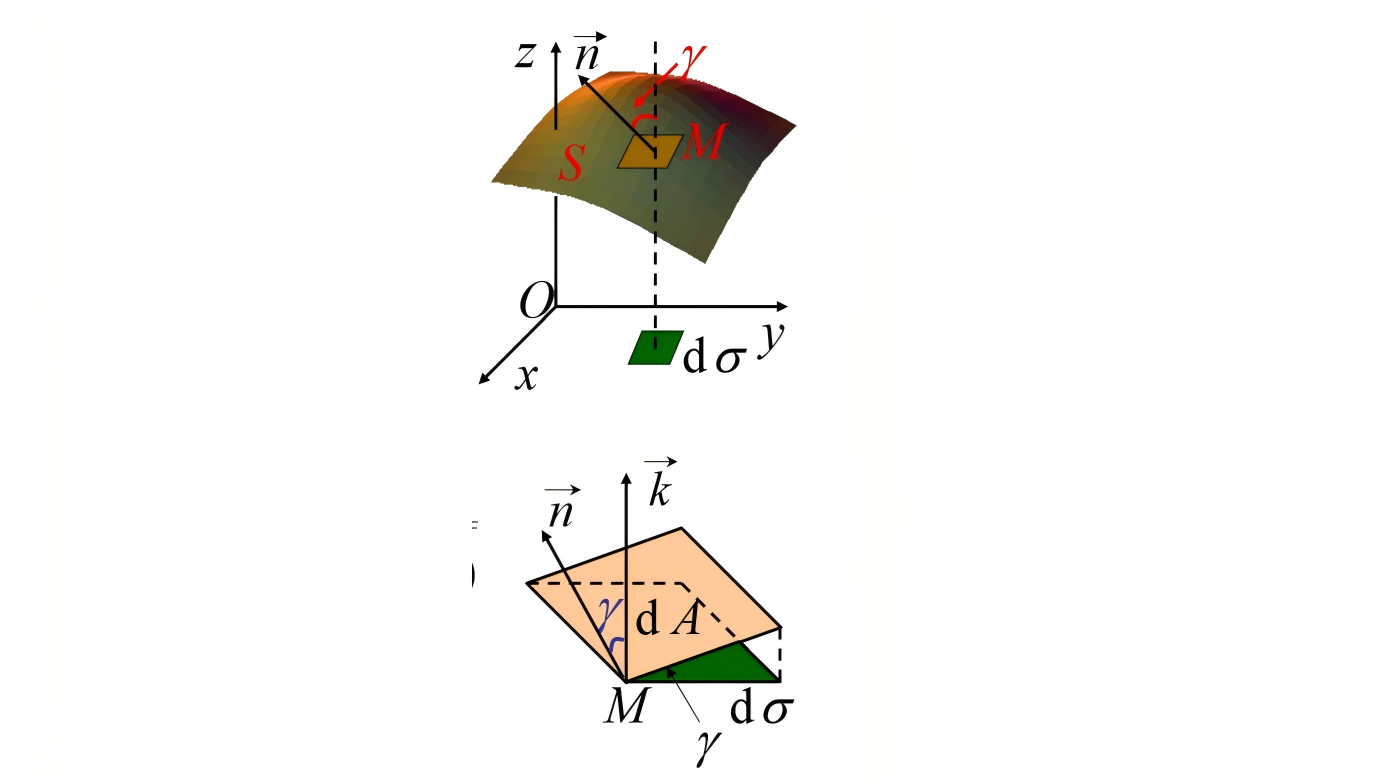
\includegraphics[width=0.86\textwidth,height=0.74\textheight,keepaspectratio]{figures/notes-md/N-20260615/N-20260615-fig-01-surface-area-element-and-projection.png}
\caption{A surface area element and its projection.  The factor between \(dS\) and the projected area element is determined by the angle between the surface normal and the projection direction.}
\end{figure}

\section{Template surfaces}

The original note lists the common templates, and they should be kept because they prevent repeated derivations.

For a plane $z=ax+by+c$,
\[
  dS=\sqrt{1+a^2+b^2}\,dx\,dy.
\]
For a sphere $x^2+y^2+z^2=R^2$, spherical coordinates give
\[
  dS=R^2\sin\varphi\,d\varphi\,d\theta.
\]
For a cylinder $x=R\cos\theta$, $y=R\sin\theta$, $z=z$,
\[
  dS=R\,d\theta\,dz.
\]
For a cone $z=\sqrt{x^2+y^2}$, use $x=r\cos\theta$, $y=r\sin\theta$, $z=r$, so
\[
  |r_r\times r_\theta|=\sqrt2\,r.
\]


\begin{figure}[H]
\centering
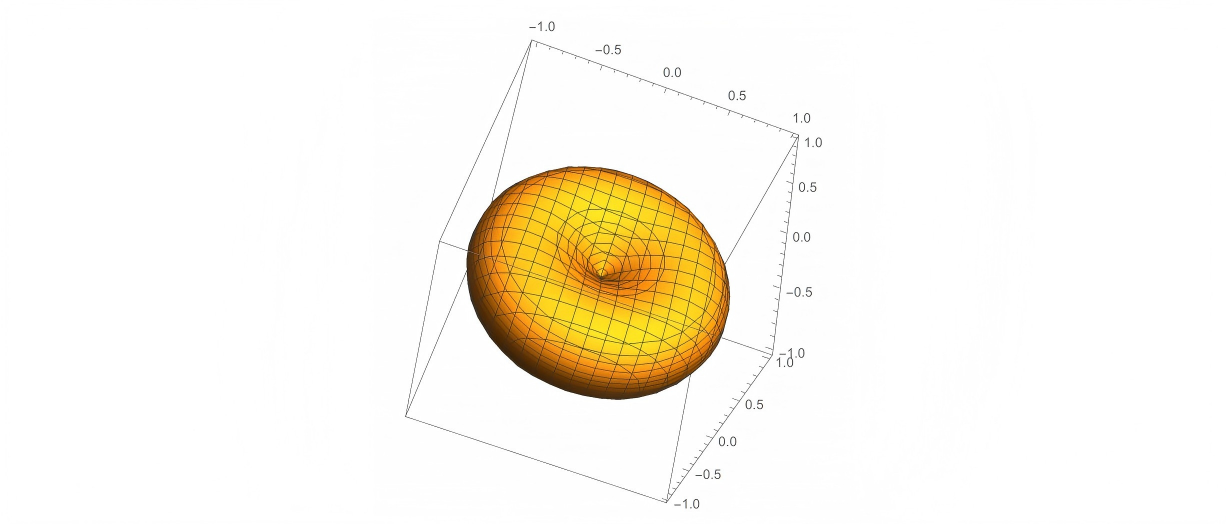
\includegraphics[width=0.70\textwidth,height=0.74\textheight,keepaspectratio]{figures/notes-md/N-20260615/N-20260615-fig-04-torus-example-surface.png}
\caption{A torus as a standard example of a parametrized surface.}
\end{figure}

\section{Example pattern: spherical cap}

For a spherical cap on $x^2+y^2+z^2=R^2$, the scalar integral of $f$ should normally be written in spherical coordinates.  If the cap is cut by $z=h$, then $z=R\cos\varphi$ gives
\[
  0\le\varphi\le \arccos(h/R).
\]
Thus
\[
  \iint_S f\,dS=
  \int_0^{2\pi}\int_0^{\arccos(h/R)}
  f(R\sin\varphi\cos\theta,R\sin\varphi\sin\theta,R\cos\varphi)
  R^2\sin\varphi\,d\varphi\,d\theta.
\]
The important part of the example is not the final antiderivative.  It is recognizing the right parameter domain.

\begin{figure}[H]
\centering
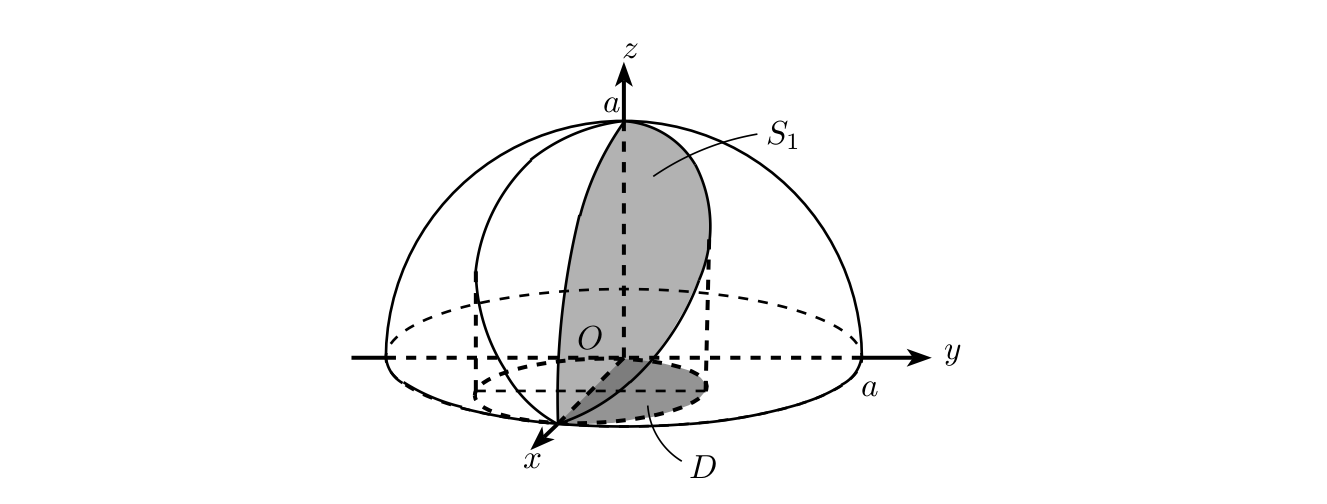
\includegraphics[width=0.78\textwidth,height=0.74\textheight,keepaspectratio]{figures/notes-md/N-20260615/N-20260615-fig-02-spherical-surface-patch-and-projection-domain.png}
\caption{A spherical surface patch and its projection domain.  This is the geometric model behind many spherical-cap surface integrals.}
\end{figure}

\begin{figure}[H]
\centering
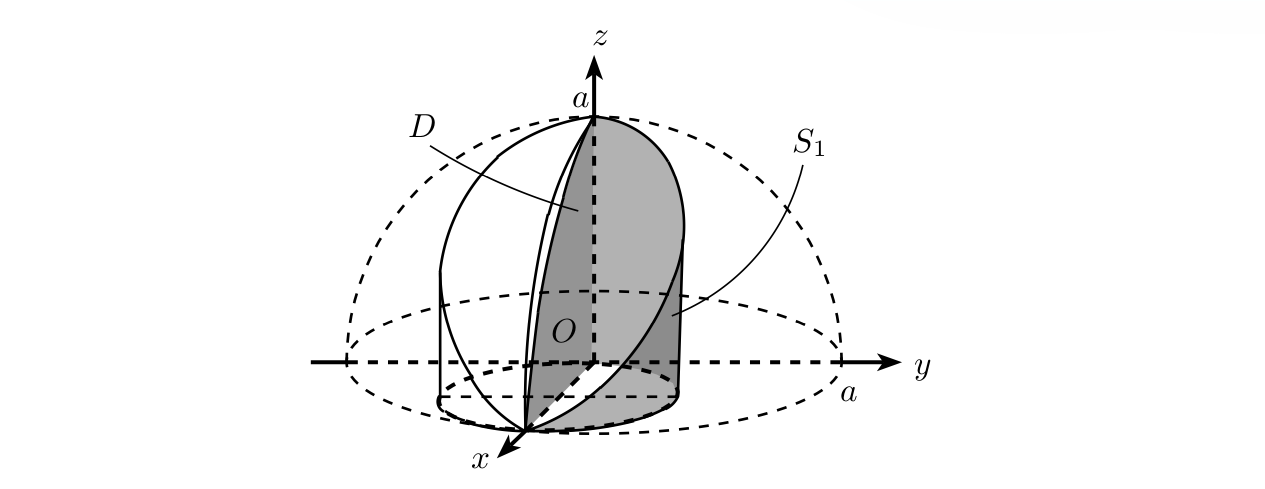
\includegraphics[width=0.78\textwidth,height=0.74\textheight,keepaspectratio]{figures/notes-md/N-20260615/N-20260615-fig-03-spherical-surface-with-bounding-cylinder.png}
\caption{A related spherical surface cut out by a vertical boundary.  The dashed curves indicate the hidden projection and bounding geometry.}
\end{figure}





\section{Second-kind surface integrals as flux}

Let $F=(P,Q,R)$.  The flux through an oriented surface $S$ is
\[
  \iint_S F\cdot n\,dS.
\]
In differential notation this is
\[
  \iint_S P\,dy\,dz+Q\,dz\,dx+R\,dx\,dy.
\]
For a parametrization $r(u,v)$,
\[
  \iint_S F\cdot n\,dS
  =\iint_D F(r(u,v))\cdot(r_u\times r_v)\,du\,dv,
\]
where the order of $u,v$ determines orientation.

For a graph $z=z(x,y)$ with upward orientation,
\[
  n\,dS=(-z_x,-z_y,1)\,dx\,dy,
\]
so
\[
  \iint_S F\cdot n\,dS
  =\iint_D[-Pz_x-Qz_y+R]\,dx\,dy.
\]
For downward orientation, change the sign.

\section{Typical flux examples from the source}

The original long note includes sphere, cone, shifted sphere, rectangular box, and partial-sphere examples.  The common structures are these.

For a sphere with outward orientation, direct parametrization works, but Gauss' theorem is often shorter if the surface is closed.  For a cone with upper orientation, the graph formula or cone parametrization should be used; the sign is the main danger.  For a shifted sphere such as
\[
  (x-a)^2+y^2+z^2=R^2,
\]
translation changes the integrand but not the geometric idea.  For a rectangular box, flux splits over six faces unless Gauss' theorem turns it into one volume integral.  For a sphere piece with only $dx\,dy$, the projection to the $xy$-plane and the sign of the normal decide whether the upper and lower sheets add or cancel.

\section{Gauss theorem}

Let $\Omega$ be a solid with outward boundary $\partial\Omega$.  For $F=(P,Q,R)$,
\[
  \iint_{\partial\Omega}F\cdot n\,dS
  =
  \iiint_\Omega (P_x+Q_y+R_z)\,dV.
\]
The divergence
\[
  \nabla\cdot F=P_x+Q_y+R_z
\]
measures local source strength.  Gauss' theorem says that total source inside equals outward flux through the boundary.

Use Gauss when the surface is closed, or when it can be closed by adding a simple cap.  If the required surface is not closed, compute the closed flux and subtract the flux across the added part.  If the problem asks for inward orientation, multiply the outward result by $-1$.

\section{Singular fields and missing points}

The note includes the important example type where the field is singular at a point.  Gauss' theorem cannot be applied across a singularity.  The usual remedy is to remove a small sphere around the singular point, apply Gauss' theorem to the punctured region, and then let the radius tend to zero.  For inverse-square radial fields, the flux through the small sphere often remains nonzero.  This is the analytic origin of point charges and delta-type sources.

\section{Stokes theorem}

Let $S$ be an oriented surface with boundary $\partial S$.  Then
\[
  \oint_{\partial S}F\cdot dr
  =
  \iint_S (\nabla\times F)\cdot n\,dS.
\]
Here
\[
  \nabla\times F=
  \begin{vmatrix}
  i&j&k\\
  \partial_x&\partial_y&\partial_z\\
  P&Q&R
  \end{vmatrix}.
\]
The right-hand rule fixes orientation: if the thumb points along $n$, the fingers curl in the positive boundary direction.

Use Stokes when the boundary curve is complicated but some spanning surface is simple, or when the curl is much simpler than the original vector field.  The surface can be changed as long as the boundary and orientation are preserved.

\section{Examples preserved from the long note}

For a triangular boundary in a plane, Stokes lets us replace a line integral over three edges by a surface integral over the triangle.  If the curl is constant, the result is just the dot product of the curl with the oriented area vector.

For an elliptical boundary, choose the planar elliptical disk rather than the original curved surface when allowed.  Parameterizing the ellipse directly is usually longer; Stokes rewards choosing the simplest spanning surface.

\section{Decision table}

\begin{center}
\begin{tabular}{lll}
\toprule
Object & Meaning & Best tool \\
\midrule
$\iint_S f\,dS$ & scalar density on surface & parametrization or graph $dS$ \\
$\iint_SF\cdot n\,dS$ & flux through oriented surface & graph formula or Gauss \\
closed flux & total outward flow & Gauss theorem \\
line circulation & work/circulation along boundary & direct line integral or Stokes \\
\bottomrule
\end{tabular}
\end{center}

\section{Conceptual endpoint}

The high-level statement is the boundary principle:
\[
  \int_{\partial M}\omega=\int_M d\omega.
\]
Green, Gauss, and Stokes are all versions of this formula.  The old vector-calculus notation hides the unity; differential forms reveal it.  The derivative $d\omega$ records local change inside a region, and the boundary integral records the accumulated effect at the edge.

\section{Elementary-to-advanced bridge: general Stokes theorem}

The vector-calculus theorems in this note are all cases of the general Stokes theorem.  If $M$ is an oriented smooth manifold with boundary and $\omega$ is a compactly supported differential form of degree one less than $\dim M$, then
\[
  \int_{\partial M}\omega=\int_M d\omega.
\]

Green's theorem, Stokes' theorem, and Gauss' theorem correspond to different degrees and dimensions:
\[
  \begin{array}{lll}
  \text{Green} & M\subseteq\mathbb R^2 & \omega=Pdx+Qdy,\\
  \text{Stokes} & M\text{ a surface in }\mathbb R^3 & \omega=Pdx+Qdy+Rdz,\\
  \text{Gauss} & M\subseteq\mathbb R^3 & \omega=Pdy\wedge dz+Qdz\wedge dx+Rdx\wedge dy.
  \end{array}
\]
The apparently different vector formulas are one theorem written in different degrees.

\section{Elementary-to-advanced bridge: singular sources and distributions}

The note mentions singular fields and missing points.  The advanced language for point sources is distribution theory.  The Dirac delta $\delta_0$ is not an ordinary function but satisfies
\[
  \int \delta_0 \varphi=\varphi(0)
\]
for test functions $\varphi$.

For the inverse-square field in $\mathbb R^3$,
\[
  F(x)=\frac{x}{|x|^3},
\]
one has classically $\nabla\cdot F=0$ away from the origin, but distributionally
\[
  \nabla\cdot F=4\pi \delta_0.
\]
This reconciles the nonzero flux through spheres with zero ordinary divergence away from the singularity.

\section{Elementary-to-advanced bridge: conservation laws}

Many PDEs have conservation-law form
\[
  \partial_t \rho+\nabla\cdot J=0.
\]
Integrating over a region $\Omega$ and applying Gauss' theorem gives
\[
  \frac d{dt}\int_\Omega \rho\,dV=-\iint_{\partial\Omega}J\cdot n\,dS.
\]
Change inside equals negative outward flux.  Thus Gauss' theorem is the geometric mechanism behind conservation of mass, charge, and probability.

\section{Elementary-to-advanced bridge: currents}

A current generalizes an oriented submanifold by acting on differential forms.  An oriented curve $C$ defines a current
\[
  T_C(\omega)=\int_C \omega.
\]
The boundary of a current is defined by
\[
  \partial T(\omega)=T(d\omega).
\]
This extends Stokes' theorem to singular chains, weak surfaces, and geometric measure theory.

The elementary surface and curve integrals in the note are therefore the smooth case of a much more flexible integration theory over generalized geometric objects.

% Second-pass deepening for waves 2-4: wave 4 part 3
\section{Second-pass deepening: Gauss and Stokes as dual local-to-global laws}

Gauss' theorem and Stokes' theorem are both local-to-global principles.  Gauss says that local source density accumulates to boundary flux.  Stokes says that local rotation accumulates to boundary circulation.  In differential-form notation, both are one formula:
\[
  \int_{\partial M}\omega=\int_M d\omega.
\]
The difference lies only in the degree of the form and the dimension of the manifold.

This unification matters because it prevents memorizing vector identities as separate facts.  The object being integrated determines the theorem: a one-form over a boundary curve gives curl through a surface; a two-form over a closed surface gives divergence through a volume.

\section{Second-pass deepening: weak forms and PDE}

In PDE, integration by parts and Stokes-type formulas define weak solutions.  Instead of requiring derivatives to exist pointwise, one tests against smooth functions.  For example, a weak divergence equation is read through
\[
  \int_\Omega F\cdot \nabla \varphi\,dV=-\int_\Omega (\nabla\cdot F)\varphi\,dV
\]
up to boundary terms.

Thus vector-calculus integral theorems are not merely computational shortcuts; they are the foundation of weak formulations, conservation laws, and modern PDE theory.



\part{Complex Analysis and Equations}
\label{vol:11-complex-analysis-and-equations}
\begingroup
\small
\sloppy
\parttoc
\endgroup

\input{tex/volumes/vol-11-complex-analysis-and-equations}

\part{Geometry and Trigonometry}
\label{vol:12-geometry-and-trigonometry}
\begingroup
\small
\sloppy
\parttoc
\endgroup

% This file is generated during volume reorganization.
% Volume: Geometry and Trigonometry

\include{tex/notes/N-20220615}
\include{tex/notes/N-20220708}
\include{tex/notes/N-20220715}
\notechapter{N-20220716}{Conic Exercises: Lines, Ellipses, Parabolas, and Tangents}

\section{Line and ellipse}

The note continues the conic-section exercises.  A line and an ellipse can have three possible positional relationships:
\[
\begin{aligned}
  \Delta>0&:\ \text{two intersections},\\
  \Delta=0&:\ \text{tangent},\\
  \Delta<0&:\ \text{no real intersection}.
\end{aligned}
\]
This is obtained by substituting the line equation into the conic equation and examining the discriminant of the resulting quadratic.

For example, consider
\[
  y=2x-2,\qquad
  \frac{x^2}{5}+\frac{y^2}{4}=1.
\]
Substitution gives
\[
  \frac{x^2}{5}+\frac{(2x-2)^2}{4}=1,
\]
so
\[
  \frac65x^2-2x=0.
\]
Thus
\[
  x=0,\qquad x=\frac53,
\]
and the intersection points are
\[
  (0,-2),\qquad \left(\frac53,\frac43\right).
\]

\section{Tangents from a point to an ellipse}

Let
\[
  C:\frac{x^2}{a^2}+\frac{y^2}{b^2}=1
\]
and let \(P=(0,2)\).  A line through \(P\) has equation
\[
  y=kx+2.
\]
Substituting into the ellipse gives a quadratic in \(x\).  Tangency occurs exactly when the discriminant is zero.

For the example on the page, this produces
\[
  k=\pm\frac{\sqrt6}{3},
\]
so the two tangents are
\[
  y=\frac{\sqrt6}{3}x+2,\qquad
  y=-\frac{\sqrt6}{3}x+2.
\]

\section{Line and hyperbola}

For the hyperbola
\[
  \frac{x^2}{2}-\frac{y^2}{2}=1,
\]
and the line
\[
  y=x-1,
\]
substitution gives
\[
  x^2-(x-1)^2=2.
\]
Hence
\[
  2x-1=2,\qquad x=\frac32,\qquad y=\frac12.
\]
The line is not tangent; it meets the hyperbola at one point because the equation degenerates to a linear equation after substitution.  This is a useful warning: for hyperbolas, ``one intersection'' need not mean tangency, because the line may be parallel to an asymptotic direction.

\section{Parabola tangent through a point}

For the parabola
\[
  x^2=\frac12 y,
\]
we have
\[
  y=2x^2.
\]
A line through \(P=(2,6)\) may be written
\[
  y=kx+6-2k.
\]
Tangency means that
\[
  2x^2=kx+6-2k
\]
has a repeated root.  Thus
\[
  2x^2-kx-6+2k=0,
\]
and the discriminant condition is
\[
  k^2-4\cdot2(-6+2k)=0.
\]
Solving gives
\[
  k=12,\qquad k=-4.
\]
The tangent lines are therefore
\[
  y=12x-18,\qquad y=-4x+14.
\]

\section{A parabola and a circle}

The second page considers the parabola
\[
  C:x^2=2py,\qquad p>0,
\]
with focus \(F\), and a circle
\[
  M:x^2+(y+4)^2=1.
\]
The problem asks for \(p\) when the shortest distance between \(F\) and the circle is \(4\), and then asks for a maximal triangle area using two tangents from a point \(P\) on the circle.

Since the focus of \(x^2=2py\) is
\[
  F=\left(0,\frac p2\right),
\]
and the circle has center
\[
  O=(0,-4)
\]
and radius \(1\), the distance from \(F\) to the circle is
\[
  FO-1=\left(\frac p2+4\right)-1=\frac p2+3.
\]
Setting this equal to \(4\) gives
\[
  p=2.
\]
Hence the parabola is
\[
  x^2=4y.
\]

For a tangent point \(A=(x_1,x_1^2/4)\) on \(x^2=4y\), the tangent has equation
\[
  xx_1=2(y+x_1^2/4),
\]
or
\[
  y=\frac{x_1}{2}x-
rac{x_1^2}{4}.
\]
Similarly for a second tangent point \(B=(x_2,x_2^2/4)\).  The two tangents meet at
\[
  P=\left(\frac{x_1+x_2}{2},\frac{x_1x_2}{4}\right).
\]
Using the condition that \(P\) lies on the circle gives an optimization problem for the area of triangle \(PAB\).  The computation in the page reduces it to a one-variable expression and obtains the maximum
\[
  [PAB]_{\max}=20\sqrt5.
\]

\section{An ellipse with prescribed quadrilateral area}

The final exercise considers an ellipse
\[
  E:\frac{x^2}{a^2}+\frac{y^2}{b^2}=1,\qquad a>b>0,
\]
passing through \(A=(0,-2)\).  Four vertices form a quadrilateral of area \(4\sqrt5\).  Since \(A=(0,-2)\) lies on the ellipse, \(b=2\).  The area condition gives
\[
  2ab=4\sqrt5,
\]
so
\[
  a=\sqrt5.
\]
Therefore
\[
  E:\frac{x^2}{5}+\frac{y^2}{4}=1.
\]

For the line through \(P=(0,-3)\)
\[
  \ell:y=kx-3,
\]
intersecting the ellipse at \(B,C\), the equation is
\[
  \frac{x^2}{5}+\frac{(kx-3)^2}{4}=1.
\]
This gives a quadratic in \(x\).  The condition that the line meet the ellipse in two points is
\[
  k>1\quad\text{or}\quad k<-1.
\]
The problem then studies where the chords meet the line \(y=-3\) and imposes
\[
  |PM|+|PN|\le15.
\]
The computation on the page reduces this to
\[
  |k|\le3.
\]
Combining conditions gives
\[
  k\in[-3,-1)\cup(1,3].
\]

\section{The next layer}

The page is a concentrated exercise in the algebraic method for conics: substitute a line into a conic, read the discriminant, and interpret the result geometrically.  The only subtlety is that different conics behave differently: for ellipses, one intersection usually signals tangency; for hyperbolas, a line parallel to an asymptotic direction can produce a single finite intersection without being tangent.


\paragraph{Expanded synthesis.}
For this chapter, the elementary material should be read as a study of what remains invariant when coordinates change. The earlier sections (`Line and ellipse`, `Tangents from a point to an ellipse`, `Line and hyperbola`, `Parabola tangent through a point`, `A parabola and a circle`) compute with arrays, bases, pivots, determinants, or eigenvectors; the deeper object is a linear map together with the spaces it acts on. A matrix is a representation of that map after bases have been chosen. This is why formulas such as
\[
  A' = P^{-1}AP,\qquad \widetilde A = T^{-1}AS
\]
are not cosmetic: they distinguish an intrinsic morphism from a coordinate description.

The structural hierarchy is as follows. Kernels record what a map forgets, images record what it reaches, cokernels record obstructions to solvability, and quotients record information after an equivalence has been imposed. Determinants act on the top exterior power and therefore measure oriented volume; traces are invariant under cyclic rearrangement and become characters in representation theory; adjoints depend on an inner product and lead to self-adjoint spectral theory.

A useful way to return to the computations is to ask, for every formula, which invariant it is measuring. Row reduction measures rank and kernel; diagonalization measures decomposition into invariant subspaces; Gram--Schmidt measures orthogonal projection; positive definiteness measures ellipsoid geometry; tensor notation measures how components transform. The elementary methods are therefore the finite-dimensional laboratory in which duality, quotienting, functoriality, and spectral decomposition can be seen clearly.


\section{Discriminants as geometric detectors}

A line intersecting a conic becomes a quadratic equation after substitution.  The discriminant is therefore a geometric detector: positive means two intersections, zero often means tangency, and negative means no real intersection.  The word ``often'' matters because hyperbolas have asymptotic directions; a line can meet a hyperbola in only one finite point without being tangent.

This is why the same algebraic method must still be interpreted geometrically.  Solving equations gives candidates, but the conic type tells us what those candidates mean.

\notechapter{N-20220719}{Solid Geometry: Points, Lines, Planes, Parallelism, and Perpendicularity}

\section{Why solid geometry feels different}

The note starts with a warning: solid geometry is not just plane geometry with one more coordinate.  The difficulty is that objects can miss each other in space.  Two lines in the plane either meet or are parallel; in space, they may also be skew.  A line can be parallel to a plane without being parallel to every line in that plane.  These small distinctions are exactly why the axioms matter.

\section{Basic axioms of incidence}

The fundamental incidence principles recorded in the note are:
\begin{enumerate}[(i)]
  \item Through three non-collinear points there is one and only one plane.
  \item If two points of a line lie in a plane, then the whole line lies in that plane.
  \item If two distinct planes have a common point, then their intersection is exactly one line through that point.
\end{enumerate}

From these one derives several useful consequences:
\begin{enumerate}[(i)]
  \item Through a line and a point not on that line, there is one and only one plane.
  \item Through two intersecting lines, there is one and only one plane.
  \item Through two parallel lines, there is one and only one plane.
\end{enumerate}

The proofs are good training in mathematical language.  One repeatedly shows existence by choosing suitable points, and uniqueness by reducing to the uniqueness of a plane through three non-collinear points.

\section{Relations between two lines}

In space, two distinct lines can be:
\begin{enumerate}[(i)]
  \item coplanar and intersecting;
  \item coplanar and parallel;
  \item non-coplanar, called skew lines.

\end{enumerate}
The first page underlines that skew lines are the genuinely new case.  Drawings can be misleading: two projected lines may cross on paper even when the actual spatial lines do not intersect.

\section{A line and a plane}

A line \(l\) and a plane \(\alpha\) have three possible relations:
\begin{enumerate}[(i)]
  \item \(l\subset\alpha\);
  \item \(l\) intersects \(\alpha\) at exactly one point;
  \item \(l\parallel\alpha\), meaning there is no common point.

\end{enumerate}

The note stresses a common mistake: a line parallel to a plane is not necessarily parallel to every line in the plane.  It is parallel to some line in the plane, but it may be skew to many others.

\section{Parallel planes and parallel lines}

Two planes are parallel if they have no common point.  The standard theorem is: if two intersecting lines in one plane are respectively parallel to two intersecting lines in another plane, then the two planes are parallel.  Conversely, if two parallel planes are cut by a third plane, the intersection lines are parallel.

This explains many of the little diagrams in the note: the right move is to find the auxiliary plane that contains the relevant lines, then reduce the spatial statement to a planar one.

\section{Perpendicularity}

A line \(l\) is perpendicular to a plane \(\alpha\) if \(l\) is perpendicular to every line in \(\alpha\) through the foot point.  The useful test is stronger-looking but easier to check:
\begin{theorem}
If a line is perpendicular to two intersecting lines in a plane, then it is perpendicular to the plane.
\end{theorem}

Once a line is perpendicular to a plane, it is perpendicular to every line in that plane through the foot.  This is the basic tool behind many distance and projection problems.

\section{Projection theorem}

The note also touches the three-perpendicular theorem.  In one common form: let \(PO\perp\alpha\), let \(AB\subset\alpha\), and let \(OQ\) be the projection of \(PQ\) onto \(\alpha\).  Then perpendicularity of \(PQ\) to a line in space can be detected by perpendicularity of its projection in the plane.  Informally, right angles survive projection when the projection is taken along a perpendicular direction.

\section{A coordinate viewpoint}

Although the note is synthetic, it is useful to connect it with vectors.  A plane in \(\mathbb R^3\) can be written
\[
  ax+by+cz=d,
\]
with normal vector
\[
  n=(a,b,c).
\]
A line with direction vector \(v\) is perpendicular to the plane iff
\[
  v\parallel n.
\]
A line lies in or is parallel to the plane iff
\[
  v\cdot n=0.
\]
Thus the synthetic tests are shadows of dot-product computations.


\section{Skew lines}

In space, two lines may be neither intersecting nor parallel.  Such lines are skew.  This is the first major difference from plane geometry.  A diagram can be misleading because a projection of skew lines may appear to intersect.

To prove two lines are skew, one usually shows they are not parallel and that the system of equations for intersection has no solution.  In vector form, lines
\[
  p+tu,\qquad q+sv
\]
intersect iff there exist \(s,t\) such that \(p+tu=q+sv\).

\section{Planes by normal vectors}

A plane can be described by a point \(p_0\) and a normal vector \(n\):
\[
  n\cdot(x-p_0)=0.
\]
This equation is often more useful than a picture.  Parallelism of planes becomes parallelism of normal vectors.  Perpendicularity of a line and a plane becomes parallelism between the line direction and the plane normal.

\section{Expanded synthesis and advanced context}

Solid geometry trains an important habit: always ask what ambient plane contains the objects you are comparing.  Many false arguments in space come from treating skew lines as if they were coplanar.  Later, vector algebra solves this with span and dot products; projective geometry solves it with incidence; linear algebra solves it with subspaces and dimensions.



\paragraph{Expanded synthesis.}
For this chapter, the elementary material should be read as a study of what remains invariant when coordinates change. The earlier sections (`Why solid geometry feels different`, `Basic axioms of incidence`, `Relations between two lines`, `A line and a plane`, `Parallel planes and parallel lines`) compute with arrays, bases, pivots, determinants, or eigenvectors; the deeper object is a linear map together with the spaces it acts on. A matrix is a representation of that map after bases have been chosen. This is why formulas such as
\[
  A' = P^{-1}AP,\qquad \widetilde A = T^{-1}AS
\]
are not cosmetic: they distinguish an intrinsic morphism from a coordinate description.

The structural hierarchy is as follows. Kernels record what a map forgets, images record what it reaches, cokernels record obstructions to solvability, and quotients record information after an equivalence has been imposed. Determinants act on the top exterior power and therefore measure oriented volume; traces are invariant under cyclic rearrangement and become characters in representation theory; adjoints depend on an inner product and lead to self-adjoint spectral theory.

A useful way to return to the computations is to ask, for every formula, which invariant it is measuring. Row reduction measures rank and kernel; diagonalization measures decomposition into invariant subspaces; Gram--Schmidt measures orthogonal projection; positive definiteness measures ellipsoid geometry; tensor notation measures how components transform. The elementary methods are therefore the finite-dimensional laboratory in which duality, quotienting, functoriality, and spectral decomposition can be seen clearly.


\section{Elementary-to-advanced bridge: affine geometry behind point-line-plane relations}

Solid geometry often begins with points, lines, and planes.  In affine geometry, a line through points $p,q$ is
\[
  p+t(q-p),\qquad t\in k,
\]
and a plane through $p$ with independent directions $u,v$ is
\[
  p+su+tv.
\]
Incidence questions become linear-dependence questions among direction vectors.

This explains the elementary tests: parallelism is dependence of direction vectors; coplanarity is rank at most two; intersection of planes is solving a linear system.

\section{Elementary-to-advanced bridge: projective completion}

Parallel lines do not meet in affine geometry, but they meet at points at infinity in projective geometry.  Projective space $\mathbb P^n$ consists of one-dimensional subspaces of $k^{n+1}$.  A point is written in homogeneous coordinates
\[
  [x_0:x_1:\cdots:x_n].
\]
Affine space sits inside projective space as the chart $x_0\ne0$.

Adding points at infinity makes many incidence theorems cleaner because parallel and intersecting cases become one case.

\section{Elementary-to-advanced bridge: Grassmannians}

The set of all $k$-dimensional linear subspaces of an $n$-dimensional vector space is the Grassmannian
\[
  Gr(k,n).
\]
Lines through the origin in $k^3$ form $Gr(1,3)=\mathbb P^2$.  Planes through the origin form $Gr(2,3)$.

Thus the collection of all possible directions of lines and planes is itself a geometric space.  The elementary act of choosing a line direction is a point in a Grassmannian.

\section{Elementary-to-advanced bridge: exterior algebra and incidence}

A line direction spanned by $u$ and a plane direction spanned by $v,w$ can be encoded by wedge products:
\[
  u,\qquad v\wedge w.
\]
Incidence conditions become wedge equations.  For example, $u$ lies in the plane spanned by $v,w$ iff
\[
  u\wedge v\wedge w=0.
\]
This gives a coordinate-free version of determinant tests for coplanarity.

\section{Returning to solid geometry}

The original point-line-plane exercises are exactly the practical computations needed for affine and projective geometry.  Direction vectors become points in Grassmannians; determinant tests become wedge-product incidence; parallel cases become ordinary intersections after projective completion.

% Second-pass deepening for waves 2-4: wave 4 part 1
\section{Second-pass deepening: incidence via ranks}

In three-dimensional analytic geometry, incidence conditions are rank conditions.  Points $P_0,P_1,P_2,P_3$ are coplanar iff the direction vectors
\[
  P_1-P_0,\quad P_2-P_0,\quad P_3-P_0
\]
are linearly dependent.  Equivalently, the determinant formed by these three vectors is zero.

A line intersects a plane when the linear system consisting of the line equation and plane equation is solvable.  A line is parallel to a plane when its direction vector lies in the kernel of the plane's normal functional.  These are all linear-algebraic conditions.

\section{Second-pass deepening: projective duality of points and planes}

In projective three-space, a plane is given by a linear equation
\[
  a_0X_0+a_1X_1+a_2X_2+a_3X_3=0.
\]
Thus planes correspond to covectors up to scale, i.e. points in the dual projective space.  Point-plane incidence is the pairing
\[
  \ell(P)=0.
\]
This duality explains why many theorems about points have dual theorems about planes.

The elementary distinction between direction vectors and normal vectors is the affine shadow of vector-covector duality.

\notechapter{N-20220802}{Trigonometric Functions, Radians, Identities, and Triangle Formulas}

\section{Angles and radians}

The note begins with angles.  An angle has an initial side and a terminal side.  Rotating counterclockwise gives a positive angle; rotating clockwise gives a negative angle.  Angles differing by a full revolution represent the same terminal direction:
\[
  \theta\sim\theta+2k\pi,\qquad k\in\mathbb Z.
\]

Radian measure is defined by arc length:
\[
  \theta=\frac{s}{r}.
\]
Thus one radian is the angle subtending an arc whose length equals the radius.  Since the circumference of a circle is \(2\pi r\), one full turn is
\[
  2\pi\text{ radians}=360^\circ.
\]
Therefore
\[
  1\text{ radian}\approx57.3^\circ.
\]

\section{Sine, cosine, and tangent}

For a point \(P=(x,y)\) on the terminal side of an angle \(\alpha\), put
\[
  r=|OP|=\sqrt{x^2+y^2}.
\]
Then
\[
  \sin\alpha=\frac yr,\qquad
  \cos\alpha=\frac xr,\qquad
  \tan\alpha=\frac yx.
\]
On the unit circle, \(r=1\), so
\[
  P=(\cos\alpha,\sin\alpha).
\]
The basic identity is
\[
  \sin^2\alpha+\cos^2\alpha=1,
\]
and
\[
  \tan\alpha=\frac{\sin\alpha}{\cos\alpha}.
\]
The note's sign diagrams for \(\sin,\cos,	an\) are exactly quadrant information.

\section{Special angles}

The page computes values such as
\[
  \sin\frac{2\pi}{3}=\frac{\sqrt3}{2},\qquad
  \cos\frac{2\pi}{3}=-\frac12,\qquad
  \tan\frac{2\pi}{3}=-\sqrt3,
\]
and
\[
  \sin\frac{3\pi}{2}=-1,\qquad
  \cos\frac{3\pi}{2}=0.
\]
The method is not memorization alone: reduce to a reference angle and then use the quadrant sign.

\section{Addition formulas}

The central identity is the cosine subtraction formula:
\[
  \cos(\alpha-\beta)
  =\cos\alpha\cos\beta+\sin\alpha\sin\beta.
\]
From it one obtains
\[
  \cos(\alpha+\beta)
  =\cos\alpha\cos\beta-\sin\alpha\sin\beta,
\]
\[
  \sin(\alpha+\beta)
  =\sin\alpha\cos\beta+\cos\alpha\sin\beta,
\]
\[
  \sin(\alpha-\beta)
  =\sin\alpha\cos\beta-\cos\alpha\sin\beta.
\]
The tangent formula follows by dividing sine by cosine:
\[
  \tan(\alpha+\beta)=\frac{\tan\alpha+\tan\beta}{1-\tan\alpha\tan\beta}.
\]

The note writes these not as isolated formulas but as relations among angles on the unit circle.  That is the best way to remember them.

\section{Double-angle and half-angle formulas}

From the addition formulas:
\[
  \sin2\alpha=2\sin\alpha\cos\alpha,
\]
\[
  \cos2\alpha=\cos^2\alpha-\sin^2\alpha
  =1-2\sin^2\alpha
  =2\cos^2\alpha-1.
\]
The half-angle identities are
\[
  \sin^2\frac\alpha2=\frac{1-\cos\alpha}{2},
  \qquad
  \cos^2\frac\alpha2=\frac{1+\cos\alpha}{2}.
\]
These formulas are especially useful in integrals and triangle geometry.

\section{Graphs of trigonometric functions}

The note draws the graphs of \(y=\sin x\), \(y=\cos x\), and \(y=\tan x\).  The key facts are:
\[
  \sin(x+2\pi)=\sin x,\qquad \cos(x+2\pi)=\cos x,
\]
\[
  \tan(x+\pi)=\tan x.
\]
Sine and cosine are bounded between \(-1\) and \(1\); tangent has vertical asymptotes at
\[
  x=\frac\pi2+k\pi.
\]

\section{Triangle formulas}

For a triangle \(ABC\) with sides \(a,b,c\) opposite the corresponding angles, the law of sines is
\[
  \frac a{\sin A}=\frac b{\sin B}=\frac c{\sin C}=2R,
\]
where \(R\) is the circumradius.

The area formulas include
\[
  [ABC]=\frac12bc\sin A
\]
and Heron's formula
\[
  [ABC]=\sqrt{s(s-a)(s-b)(s-c)},\qquad s=\frac{a+b+c}{2}.
\]

The note also records trigonometric transformations involving sums of angles in a triangle, especially \(A+B+C=\pi\).  For example,
\[
  \sin(A+B)=\sin C,\qquad \cos(A+B)=-\cos C.
\]


\section{Radians are not a convention only}

The radian measure of an angle is defined by arc length divided by radius:
\[
  \theta=\frac{s}{r}.
\]
This makes the derivative formulas clean:
\[
  \frac{d}{dx}\sin x=\cos x,\qquad
  \frac{d}{dx}\cos x=-\sin x.
\]
If degrees were used inside calculus, extra conversion constants would appear everywhere.  Thus radians are the natural unit for analysis.

\section{Addition formulas as rotation composition}

The matrix
\[
  R(\theta)=\begin{pmatrix}\cos\theta&-\sin\theta\\ \sin\theta&\cos\theta\end{pmatrix}
\]
rotates the plane by \(\theta\).  Since rotations compose by adding angles,
\[
  R(\alpha+\beta)=R(\alpha)R(\beta).
\]
Multiplying the matrices gives the sine and cosine addition formulas.  This explains why those identities are not arbitrary memorized formulas but the algebra of rotations.

\section{From technique to structure}

Trigonometry is not just a table of identities.  It is the coordinate algebra of the circle.  Radians measure angle by arc length; sine and cosine are coordinates on the unit circle; addition formulas express rotation composition; triangle formulas translate between angle data and side data.  This is why trigonometry becomes natural again in complex numbers, Fourier analysis, rotations, and differential equations.

\section{Radians and the exponential map}

Radians are natural because arc length on the unit circle equals angle.  The map
\[
  t\mapsto e^{it}
\]
wraps the real line around the circle, and addition of angles becomes multiplication of complex numbers.

This is the structural source of the addition formulas for sine and cosine.

\section{Addition formulas from rotation matrices}

The rotation matrix
\[
  R(t)=\begin{pmatrix}\cos t&-\sin t\\\sin t&\cos t\end{pmatrix}
\]
satisfies
\[
  R(s+t)=R(s)R(t).
\]
Multiplying matrices gives the sine and cosine addition formulas.  Thus the identities express composition of rotations.

\section{Triangle formulas and invariant quantities}

The sine rule and cosine rule relate side lengths and angles.  The cosine rule is an inner-product identity:
\[
  c^2=a^2+b^2-2ab\cos C.
\]
It is the law of dot products written in triangle language.

\section{Trigonometry as rotation geometry}

Trigonometry is geometry of the circle and rotations.  Radians come from arc length, addition formulas from group composition, graphs from periodicity, and triangle formulas from inner-product geometry.

\section{Trigonometry and rotations}

The matrix
\[
  R_\theta=\begin{pmatrix}\cos\theta&-\sin\theta\\\sin\theta&\cos\theta\end{pmatrix}
\]
represents rotation by angle $\theta$.  The identity
\[
  R_\alpha R_\beta=R_{\alpha+\beta}
\]
contains the addition formulas for sine and cosine.

Thus trigonometric identities are representation theory of the group $SO(2)$ in coordinates.

\section{Complex exponentials}

Euler's formula
\[
  e^{i\theta}=\cos\theta+i\sin\theta
\]
turns trigonometric identities into exponential algebra.  For example,
\[
  e^{i(\alpha+\beta)}=e^{i\alpha}e^{i\beta}
\]
gives both addition formulas at once.

The multiple-angle formulas are simply
\[
  (e^{i\theta})^n=e^{in\theta}.
\]
Taking real and imaginary parts yields Chebyshev-type identities:
\[
  \cos(n\theta)=T_n(\cos\theta).
\]

\section{Spherical trigonometry}

On a sphere, triangles are bounded by great-circle arcs.  Their angles and side lengths satisfy different laws from Euclidean triangles.  The spherical law of cosines is
\[
  \cos c=\cos a\cos b+\sin a\sin b\cos C.
\]
This reduces to the Euclidean law of cosines in a small-scale limit.

The elementary triangle formulas in the plane are therefore the zero-curvature case of trigonometry on constant-curvature geometries.

\section{Harmonic analysis}

Trigonometric functions form an orthogonal system.  On $[-\pi,\pi]$,
\[
  \int_{-\pi}^{\pi}\sin mx\sin nx\,dx=0
\]
for $m\ne n$, and similarly for cosines.  This is why Fourier series can decompose functions into sine and cosine modes.

The original trigonometric identities are therefore also algebra of Fourier modes.  Products of sines and cosines correspond to sums of frequencies.

\section{Trigonometric identities as algebra}

The functions $e^{in\theta}$ form characters of the circle group.  Products of trigonometric functions are products of characters, which add frequencies:
\[
  e^{im\theta}e^{in\theta}=e^{i(m+n)\theta}.
\]
The product-to-sum formulas are just this identity rewritten in real and imaginary parts.

This explains why trigonometric simplification is often frequency bookkeeping.  A complicated expression may be simplified by converting to exponentials, combining frequencies, and returning to real functions.

\section{Curvature and spherical trigonometry}

In Euclidean geometry, the angle sum of a triangle is $\pi$.  On a unit sphere, the spherical excess satisfies
\[
  A+B+C-\pi=\operatorname{area}(\triangle).
\]
Thus trigonometry detects curvature.  Plane triangle formulas are the zero-curvature limit of spherical and hyperbolic formulas.

This provides a genuine high-level extension of elementary trigonometry: identities involving sides and angles are not merely computational; they reflect the geometry of the underlying space.

\notechapter{N-20220911}{Analytic Geometry: Lines, Circles, and Coordinate Tricks}

\section{Line formulas}

This note is a formula sheet and worked exercise collection for analytic geometry.  The first part summarizes equations of a line.

If a line has inclination angle \(\alpha\), then its slope is
\[
  k=\tan\alpha,\qquad \alpha\neq\frac\pi2.
\]
If it passes through two points
\[
  P_1=(x_1,y_1),\qquad P_2=(x_2,y_2),
\]
then
\[
  k=\frac{y_2-y_1}{x_2-x_1}.
\]
The point-slope form is
\[
  y-y_1=k(x-x_1),
\]
the slope-intercept form is
\[
  y=kx+b,
\]
the two-point form is
\[
  \frac{y-y_1}{y_2-y_1}=\frac{x-x_1}{x_2-x_1},
\]
the intercept form is
\[
  \frac xa+\frac yb=1,
\]
and the general form is
\[
  Ax+By+C=0.
\]

The note's diagram of intercepts reminds us that the intercept form is convenient only when the line meets both coordinate axes away from the origin.

\section{Parallel and perpendicular lines}

For
\[
  l_1:y=k_1x+b_1,\qquad l_2:y=k_2x+b_2,
\]
we have
\[
  l_1\parallel l_2\quad\Longleftrightarrow\quad k_1=k_2,\ b_1\neq b_2,
\]
and
\[
  l_1\perp l_2\quad\Longleftrightarrow\quad k_1k_2=-1.
\]
For lines in general form,
\[
  l_1:A_1x+B_1y+C_1=0,\qquad
  l_2:A_2x+B_2y+C_2=0,
\]
parallelism is detected by proportional normal vectors:
\[
  \frac{A_1}{A_2}=\frac{B_1}{B_2}\neq\frac{C_1}{C_2},
\]
and perpendicularity is
\[
  A_1A_2+B_1B_2=0.
\]
This is just the dot product of the normal vectors.

\section{Direction and normal vectors}

For a line
\[
  Ax+By+C=0,
\]
a normal vector is
\[
  n=(A,B),
\]
and a direction vector is
\[
  d=(-B,A).
\]
Thus the vector form through \(P_0=(x_0,y_0)\) is
\[
  \frac{x-x_0}{u}=\frac{y-y_0}{v}
\]
if \(d=(u,v)\), and
\[
  a(x-x_0)+b(y-y_0)=0
\]
if \(n=(a,b)\).

This vector viewpoint is the easiest way to remember the formulas.  The line is the set of points whose displacement from \(P_0\) is perpendicular to a fixed normal vector.

\section{Angles, distances, and parallel lines}

The angle between two nonvertical lines is given by
\[
  \tan\theta=\left|\frac{k_1-k_2}{1+k_1k_2}\right|.
\]
Equivalently, using direction vectors \(d_1,d_2\),
\[
  \cos\theta=\frac{|d_1\cdot d_2|}{|d_1|\,|d_2|}.
\]

The distance between points is
\[
  |AB|=\sqrt{(x_2-x_1)^2+(y_2-y_1)^2}.
\]
The distance from a point \(P(x_0,y_0)\) to a line
\[
  Ax+By+C=0
\]
is
\[
  d=\frac{|Ax_0+By_0+C|}{\sqrt{A^2+B^2}}.
\]
For parallel lines
\[
  Ax+By+C_1=0,\qquad Ax+By+C_2=0,
\]
the distance is
\[
  d=\frac{|C_1-C_2|}{\sqrt{A^2+B^2}}.
\]

\section{Circle equations}

A circle with center \(C(a,b)\) and radius \(r\) has equation
\[
  (x-a)^2+(y-b)^2=r^2.
\]
The general equation is
\[
  x^2+y^2+Dx+Ey+F=0.
\]
Completing the square gives
\[
  \left(x+\frac D2\right)^2+\left(y+\frac E2\right)^2
  =\frac{D^2+E^2-4F}{4}.
\]
Hence the center is
\[
  \left(-\frac D2,-\frac E2\right),
\]
and it is a real circle exactly when
\[
  D^2+E^2-4F>0.
\]

The handwritten note underlines this discriminant-like quantity because forgetting it leads to treating imaginary circles as real ones.

\section{A fractional-linear range problem}

One example asks for the range of
\[
  \mu=\frac{x}{y-3}
\]
under
\[
  |x|+|y|\le1.
\]
The idea is geometric.  The equation
\[
  \mu=\frac{x}{y-3}
\]
can be rewritten as
\[
  x=\mu(y-3).
\]
For fixed \(\mu\), this is a line through the point \((0,3)\).  The range of \(\mu\) is determined by which slopes make this line intersect the diamond
\[
  |x|+|y|\le1.
\]
The boundary slopes give
\[
  \mu\in\left[-\frac13,\frac13\right].
\]
The note draws the diamond because the range is easier to see as a family of lines than as an algebraic fraction.

\section{A graph-slope counting problem}

Another exercise asks for the number of \(x_i\) such that
\[
  \frac{f(x_i)}{x_i}
\]
has a fixed value.  Geometrically, the ratio \(f(x)/x\) is the slope of the line from the origin to the point \((x,f(x))\).  So the problem asks how many times a line through the origin can be tangent or secant to the drawn curve with a given slope.  The answer is read from the graph, not from algebraic manipulation.

This is a useful change of viewpoint: ratios involving \(y/x\) often mean slopes of rays from the origin.

\section{A moving-line maximum}

A later problem has moving lines through fixed points \(A=(-3,0)\) and \(B=(1,6)\), intersecting at \(P\), and asks for the maximum of
\[
  |PA|\cdot |PB|.
\]
The solution uses a right-angle configuration.  Since the two moving lines are perpendicular, \(P\) lies on the circle with diameter \(AB\).  Then
\[
  |PA|^2+|PB|^2=|AB|^2.
\]
Thus
\[
  |PA||PB|\le\frac{|PA|^2+|PB|^2}{2}=\frac{|AB|^2}{2}.
\]
This is equality when \(PA=PB\).  With
\[
  |AB|^2=(1+3)^2+6^2=52,
\]
the maximum is
\[
  26.
\]

\section{Triangle coordinate problem}

The final worked example gives \(A=(5,1)\), the median line \(CM\), and the perpendicular bisector \(BN\), then asks for \(B\) and the equation of \(BC\).  The handwritten solution introduces unknown coordinates and uses two facts:
\begin{enumerate}[(i)]
  \item a median means a midpoint condition;
  \item a perpendicular bisector means equal distances or perpendicular slopes.

\end{enumerate}
Coordinate geometry often works this way: translate each geometric phrase into an equation, then solve the resulting system.


\section{Coordinate tricks as changes of viewpoint}

Analytic geometry often becomes simple after choosing better coordinates.  A line is easiest when written in point-direction form,
\[
  p+tv,
\]
while a circle is easiest when written by center and radius,
\[
  (x-a)^2+(y-b)^2=r^2.
\]
Expanding too early hides the geometry.  Completing the square recovers it.

\section{Power of a point}

For a circle with center \(O\) and radius \(r\), the power of a point \(P\) is
\[
  OP^2-r^2.
\]
If a line through \(P\) meets the circle at \(A,B\), then
\[
  PA\cdot PB
\]
is constant.  This is a standard way to convert circle intersection geometry into algebraic length equations.

\section{The structural moral}

Analytic geometry is not merely a bag of formulas.  Each formula has a vector meaning: slope is direction, \(Ax+By+C=0\) encodes a normal vector, distance to a line is projection onto that normal vector, and circle equations are completed squares.  The more one sees these meanings, the less one needs to memorize.



\paragraph{Expanded synthesis.}
For this chapter, the elementary material should be read as a study of what remains invariant when coordinates change. The earlier sections (`Line formulas`, `Parallel and perpendicular lines`, `Direction and normal vectors`, `Angles, distances, and parallel lines`, `Circle equations`) compute with arrays, bases, pivots, determinants, or eigenvectors; the deeper object is a linear map together with the spaces it acts on. A matrix is a representation of that map after bases have been chosen. This is why formulas such as
\[
  A' = P^{-1}AP,\qquad \widetilde A = T^{-1}AS
\]
are not cosmetic: they distinguish an intrinsic morphism from a coordinate description.

The structural hierarchy is as follows. Kernels record what a map forgets, images record what it reaches, cokernels record obstructions to solvability, and quotients record information after an equivalence has been imposed. Determinants act on the top exterior power and therefore measure oriented volume; traces are invariant under cyclic rearrangement and become characters in representation theory; adjoints depend on an inner product and lead to self-adjoint spectral theory.

A useful way to return to the computations is to ask, for every formula, which invariant it is measuring. Row reduction measures rank and kernel; diagonalization measures decomposition into invariant subspaces; Gram--Schmidt measures orthogonal projection; positive definiteness measures ellipsoid geometry; tensor notation measures how components transform. The elementary methods are therefore the finite-dimensional laboratory in which duality, quotienting, functoriality, and spectral decomposition can be seen clearly.


\section{Conics as quadratic forms}

A conic in the plane has equation
\[
  ax^2+2bxy+cy^2+dx+ey+f=0.
\]
The quadratic part is the symmetric matrix
\[
  Q=\begin{pmatrix}a&b\\b&c\end{pmatrix}.
\]
Orthogonal diagonalization of $Q$ removes the $xy$ term.  Translation then attempts to remove linear terms.  This is the linear-algebraic classification behind the elementary conic formulas.

The discriminant
\[
  b^2-ac
\]
distinguishes ellipse, parabola, and hyperbola types in the nondegenerate real case.  In projective geometry, these distinctions are understood through rank and intersection with the line at infinity.

\section{Affine transformations}

An affine transformation has the form
\[
  x\mapsto Ax+b,\qquad A\in GL(n).
\]
It sends lines to lines and preserves ratios along a line, but not necessarily distances or angles.  Many analytic-geometry simplifications are affine changes of coordinates.

Under affine transformations, ellipses may be transformed into circles, and general nondegenerate conics may be brought to standard forms.  The elementary completion-of-squares method is one coordinate expression of this broader equivalence.

\section{Projective viewpoint on conics}

Using homogeneous coordinates $[X:Y:Z]$, a conic is given by a homogeneous quadratic equation
\[
  \begin{pmatrix}X&Y&Z\end{pmatrix}A\begin{pmatrix}X\\Y\\Z\end{pmatrix}=0.
\]
Projective transformations act by
\[
  A\mapsto P^TAP.
\]
This unifies ellipses, parabolas, and hyperbolas over the complex projective plane; the affine differences come from how the conic meets the line at infinity $Z=0$.

\section{Duality}

In projective geometry, points and lines have a dual relationship.  A nondegenerate conic identifies points with polar lines.  If a conic is represented by a symmetric matrix $A$, the polar line of a point $p$ is
\[
  p^TAx=0.
\]
This gives an advanced interpretation of tangents and chord relations.

\section{Returning to analytic geometry}

The original formulas for lines, circles, and conics remain the computational core.  The advanced layer says: lines are affine/projective objects, conics are quadratic forms, coordinate changes are group actions, and tangents/polars come from bilinear algebra.

% Second-pass deepening for waves 2-4: wave 4 part 1
\section{Distance formulas as dual norms}

The distance from a point $x_0$ to a line
\[
  ax+by+c=0
\]
is
\[
  \frac{|ax_0+by_0+c|}{\sqrt{a^2+b^2}}.
\]
The numerator evaluates an affine functional; the denominator is the norm of its linear part.  In normed-space language, distance to a hyperplane uses the dual norm of the defining functional.

For a hyperplane $\varphi(x)=c$ in an inner product space,
\[
  \operatorname{dist}(x_0,H)=\frac{|\varphi(x_0)-c|}{\|\varphi\|_*}.
\]
In Euclidean coordinates, $\|\varphi\|_*$ is the length of the normal vector.

\section{Conics and degenerations}

A conic represented by a symmetric homogeneous matrix $A$ may be nondegenerate or degenerate.  Degenerate conics include pairs of lines, double lines, or points over the real affine plane.  Algebraically, degeneracy corresponds to rank drop of $A$.

This gives a unified view of many analytic-geometry cases: a circle, ellipse, parabola, hyperbola, or pair of lines is controlled by rank, signature, and the line at infinity.  Completing squares is a coordinate method for revealing those invariants.

\notechapter{N-20230119}{Plane Geometry I: Ceva, Menelaus, Ptolemy, Simson Line, and Euler Line}

\section{Why this geometry chapter matters}

The note is a chapter-style plane geometry note.  It does not merely list named theorems; it gives statements, pictures, proofs, and comments about when each theorem is useful.  The main pattern is:
\[
\begin{gathered}
  \text{Ceva detects concurrence},\quad
  \text{Menelaus detects collinearity},\\
  \text{Ptolemy detects cyclicity}.
\end{gathered}
\]
Then Simson line and Euler line enter as richer configurations involving circles, projections, centers, and ratios.

\section{Ceva's theorem}

Let $D,E,F$ lie on $BC,CA,AB$ or their extensions in triangle $ABC$.  Ceva's theorem says that $AD,BE,CF$ are concurrent iff
\[
  \frac{BD}{DC}\cdot \frac{CE}{EA}\cdot \frac{AF}{FB}=1
\]
using directed lengths.

The proof in the note uses areas.  Suppose the cevians meet at $O$.  Since triangles with bases on the same line and the same altitude have areas proportional to their bases,
\[
  \frac{BD}{DC}=\frac{[ABD]}{[ACD]}=\frac{[OBD]}{[OCD]}.
\]
Subtracting the smaller triangles gives
\[
  \frac{[ABO]}{[ACO]}=\frac{BD}{DC}.
\]
Similarly,
\[
  \frac{[BCO]}{[BAO]}=\frac{CE}{EA},\qquad
  \frac{[CAO]}{[CBO]}=\frac{AF}{FB}.
\]
Multiplying the three identities cancels all area factors and gives the Ceva product $1$.

The inverse theorem is often the useful direction: if the product of ratios is $1$, then the three cevians are concurrent.  In olympiad geometry, this is the standard tool for proving three lines meet at one point.

\section{Menelaus' theorem}

Menelaus is the collinearity counterpart of Ceva.  If a line meets the sidelines of triangle $ABC$ at $D,E,F$, then
\[
  \frac{AE}{EC}\cdot \frac{CD}{DB}\cdot \frac{BF}{FA}=1
\]
again with directed lengths.

The proof in the original note draws a parallel through a vertex.  For instance, draw through $B$ a line parallel to the transversal and compare similar triangles.  The ratios on the sides of the triangle become ratios on a pair of parallel lines.  After substitution, the product becomes $1$.

The memory rule is useful but not enough: Ceva and Menelaus look similar, so one must remember what they prove.  Ceva: three cevians concurrent.  Menelaus: three points collinear.

\section{Ptolemy's theorem}

For a cyclic quadrilateral $ABCD$, Ptolemy's theorem states
\[
  AC\cdot BD=AB\cdot CD+AD\cdot BC.
\]
The note also records the converse: if a convex quadrilateral satisfies this equality, then it is cyclic.

A classical proof chooses a point or diagonal construction so that two pairs of triangles become similar.  The products $AB\cdot CD$ and $AD\cdot BC$ then appear as pieces of $AC\cdot BD$.  What matters is that cyclicity converts equal angles into similarity.

Ptolemy is metric: it relates lengths, not only ratios.  That is why it is more rigid than Ceva or Menelaus.

\section{Generalized Ptolemy inequality}

For any convex quadrilateral $ABCD$, the generalized Ptolemy inequality says
\[
  AC\cdot BD\le AB\cdot CD+AD\cdot BC,
\]
with equality iff the quadrilateral is cyclic.

The note gives a complex-plane proof.  Assign complex numbers $a,b,c,d$ to the vertices.  The identity
\[
  (a-b)(c-d)+(a-d)(b-c)=(a-c)(b-d)
\]
is exact.  Taking moduli and applying the triangle inequality gives
\[
  |a-c||b-d|\le |a-b||c-d|+|a-d||b-c|.
\]
This is precisely Ptolemy's inequality.  Equality in the triangle inequality corresponds to the relevant complex numbers having the same argument, which geometrically means the points are concyclic in the required order.

This proof is important because it changes the language of geometry: a quadrilateral becomes four complex numbers, and a metric inequality becomes the ordinary triangle inequality.

\section{Simson line}

Simson's theorem says: if $P$ lies on the circumcircle of triangle $ABC$, and perpendiculars are dropped from $P$ to the three sides (or their extensions), then the three feet are collinear.  The common line is the Simson line of $P$.

The proof in the note uses cyclic quadrilaterals.  Let the feet be $D,E,F$.  Because $PE\perp AB$ and $PF\perp AC$, quadrilaterals such as $AEPF$ are cyclic.  Similar cyclic-angle relations show that the angle between two of the foot segments is supplementary to the angle between another pair.  Hence the three feet lie on a line.

The inverse theorem is also true.  The practical use is: when a problem contains many perpendicular feet from a point to the sides of a triangle, look for a circumcircle point and a Simson line.

\section{Euler line and Euler formula}

For triangle $ABC$, let $O$ be the circumcenter, $G$ the centroid, and $H$ the orthocenter.  Euler's theorem says that $O,G,H$ are collinear and
\[
  OG:GH=1:2,
\]
equivalently $GH=2OG$.  This common line is the Euler line.

One proof uses midpoints and similar triangles.  Let $D$ be the midpoint of $BC$.  Since $G$ is the centroid, $AG:GD=2:1$.  Using the facts that the circumcenter lies on perpendicular bisectors and the orthocenter lies on altitudes, one constructs similar triangles showing that the point on $OH$ with the centroid ratio is exactly $G$.

The note also states Euler's formula relating the circumradius $R$, inradius $r$, and the distance $d=OI$ between circumcenter and incenter:
\[
  R^2-d^2=2Rr.
\]
This immediately gives Euler's inequality
\[
  R\ge 2r,
\]
with equality iff the triangle is equilateral.  The proof in the note uses the angle bisector through the incenter, intersections with the circumcircle, and similar triangles to derive a product relation.  The key point is that the inequality is not a random radius estimate; it is the nonnegativity of $d^2$.

\section{Why the pattern matters}

This chapter is a small map of classical geometry.  Ceva and Menelaus are ratio theorems, almost projective in flavor.  Ptolemy is metric and cyclic.  Simson line turns perpendicular projections into collinearity.  Euler line organizes triangle centers, and Euler's formula links local radii with the global placement of centers.  The proofs constantly switch languages: area, similarity, complex numbers, cyclic angles, and centers.  That switching is the real skill of plane geometry.



\paragraph{Expanded synthesis.}
For this chapter, the elementary material should be read as a study of what remains invariant when coordinates change. The earlier sections (`Why this geometry chapter matters`, `Ceva's theorem`, `Menelaus' theorem`, `Ptolemy's theorem`, `Generalized Ptolemy inequality`) compute with arrays, bases, pivots, determinants, or eigenvectors; the deeper object is a linear map together with the spaces it acts on. A matrix is a representation of that map after bases have been chosen. This is why formulas such as
\[
  A' = P^{-1}AP,\qquad \widetilde A = T^{-1}AS
\]
are not cosmetic: they distinguish an intrinsic morphism from a coordinate description.

The structural hierarchy is as follows. Kernels record what a map forgets, images record what it reaches, cokernels record obstructions to solvability, and quotients record information after an equivalence has been imposed. Determinants act on the top exterior power and therefore measure oriented volume; traces are invariant under cyclic rearrangement and become characters in representation theory; adjoints depend on an inner product and lead to self-adjoint spectral theory.

A useful way to return to the computations is to ask, for every formula, which invariant it is measuring. Row reduction measures rank and kernel; diagonalization measures decomposition into invariant subspaces; Gram--Schmidt measures orthogonal projection; positive definiteness measures ellipsoid geometry; tensor notation measures how components transform. The elementary methods are therefore the finite-dimensional laboratory in which duality, quotienting, functoriality, and spectral decomposition can be seen clearly.


\section{Barycentric coordinates}

For a triangle $ABC$, barycentric coordinates write a point $P$ as
\[
  P=\frac{\alpha A+\beta B+\gamma C}{\alpha+\beta+\gamma}.
\]
The ratios in Ceva and Menelaus are naturally expressed through barycentric coordinates.  For instance, a point on side $BC$ has coordinates $(0:\beta:\gamma)$, and the side ratio is encoded by $\beta/\gamma$.

Ceva's theorem becomes a product condition on ratios because three cevians are concurrent exactly when their barycentric coordinate equations have a common solution.

\section{Projective transformations}

Ceva, Menelaus, and many incidence theorems are projective: they remain true under projective transformations.  A projective transformation sends lines to lines and preserves incidence, but not lengths or angles.

This explains why ratio and cross-ratio methods are so powerful.  They use quantities that survive projective changes.  One may move a complicated triangle configuration to a simpler projective position, prove the statement there, and transfer it back.

\section{Ptolemy and inversive geometry}

Ptolemy's theorem characterizes cyclic quadrilaterals:
\[
  AC\cdot BD=AB\cdot CD+BC\cdot AD
\]
for a cyclic quadrilateral $ABCD$.  Inversive geometry explains why cyclic configurations are flexible.  Inversion in a circle sends generalized circles to generalized circles and preserves angles.

Many circle theorems, including Simson line configurations, become simpler after an inversion sends one circle to a line or normalizes the circumcircle.

\section{Elliptic and hyperbolic analogues}

Classical Euclidean triangle geometry has analogues in spherical and hyperbolic geometry.  Ceva-type and Menelaus-type theorems survive with trigonometric replacements.  For example, in spherical geometry, side lengths and angles interact through sine laws rather than linear ratios.

This shows which parts of theorems are affine/projective and which depend on Euclidean metric.  Ratio statements tend to be projective; angle and length statements depend more strongly on the geometry.

\section{Returning to the theorem list}

The original list of Ceva, Menelaus, Ptolemy, Simson, and Euler-line facts is not just a catalogue.  It spans three geometries: affine ratio geometry, projective incidence geometry, and inversive circle geometry.  The advanced reconstruction should keep the elementary proofs while identifying which invariance principle makes each theorem natural.

% Second-pass deepening for waves 2-4: wave 4 part 1
\section{Ceva and Menelaus as dual affine statements}

Ceva concerns concurrence of cevians; Menelaus concerns collinearity of points on sides.  In barycentric coordinates, these become dual linear-algebraic conditions.  Concurrence means three lines have a common solution.  Collinearity means three points satisfy one linear equation.

This duality is why the product of ratios appears in both theorems, with reciprocal-looking signs.  The elementary ratio-chasing proof is a coordinate proof in the affine\-/projective plane.

\section{Euler line and affine covariance}

The centroid, circumcenter, orthocenter, and nine-point center belong to metric triangle geometry, but some constructions behave well under affine maps and others do not.  The centroid is affine: it is the average of vertices.  Orthocenter and circumcenter depend on perpendicularity, so they are metric.

The Euler line therefore mixes affine and metric structures.  Understanding which points survive affine transformations clarifies why some triangle centers are more universal than others.

\section{Simson line through projection}

The Simson line theorem says that projections of a point on the circumcircle onto the three sides of a triangle are collinear.  This can be interpreted through oriented angles and cyclic quadrilaterals, but also through projective degeneration: as a point moves on the circumcircle, a family of pedal triangles degenerates exactly when the point lies on the circumcircle.

Thus the theorem is not just a miracle of angle chasing; it records a degeneracy condition in a moving geometric construction.

\notechapter{N-20230220}{Special Proofs of Trigonometric Addition Formulas}

\section{Motivation}

This handwritten note tries several proofs of trigonometric addition formulas.  The author first tried a mixed line-slope proof for tangent, then tried reciprocal bases, then settled on more reliable methods for sine and cosine.  This history is important: it records why some apparently clever approaches become awkward.

\section{Sine difference formula by geometry}

Place two unit vectors at angles \(\alpha\) and \(\beta\):
\[
  u=(\cos\alpha,\sin\alpha),\qquad v=(\cos\beta,\sin\beta).
\]
The magnitude of the two-dimensional cross product is
\[
  |u\times v|=\sin|\beta-\alpha|.
\]
But the determinant gives
\[
  u\times v=\cos\alpha\sin\beta-\sin\alpha\cos\beta.
\]
Hence, with orientation taken into account,
\[
  \sin(\beta-\alpha)=\sin\beta\cos\alpha-\cos\beta\sin\alpha.
\]

This proof is clean because the determinant already measures signed area, and signed area of two unit vectors is sine of the included angle.

\section{Rotation-matrix proof}

The rotation matrix is
\[
  R(\theta)=
  \begin{pmatrix}
  \cos\theta&-\sin\theta\\
  \sin\theta&\cos\theta
  \end{pmatrix}.
\]
Because rotating by \(\alpha\) and then by \(\beta\) is the same as rotating by \(\alpha+\beta\),
\[
  R(\alpha+\beta)=R(\beta)R(\alpha).
\]
Multiplying matrices gives
\[
  \cos(\alpha+\beta)=\cos\alpha\cos\beta-\sin\alpha\sin\beta,
\]
\[
  \sin(\alpha+\beta)=\sin\alpha\cos\beta+\cos\alpha\sin\beta.
\]
This is probably the most conceptual elementary proof: addition formulas are simply composition laws for rotations.

\section{Euler formula proof}

Euler's formula gives
\[
  e^{i\theta}=\cos\theta+i\sin\theta.
\]
Then
\[
  e^{i(\alpha+\beta)}=e^{i\alpha}e^{i\beta}.
\]
Expanding the right-hand side gives
\[
  (\cos\alpha+i\sin\alpha)(\cos\beta+i\sin\beta)
\]
\[
  =(\cos\alpha\cos\beta-\sin\alpha\sin\beta)
  +i(\sin\alpha\cos\beta+\cos\alpha\sin\beta).
\]
Equating real and imaginary parts yields the addition formulas.

\section{Tangent formula}

Once sine and cosine are known,
\[
  \tan(\alpha+\beta)=\frac{\sin(\alpha+\beta)}{\cos(\alpha+\beta)}
  =\frac{\tan\alpha+	an\beta}{1-	an\alpha\tan\beta},
\]
provided the denominators are nonzero.  This is why trying to prove tangent first is often less natural: tangent is a quotient, while sine and cosine are coordinates of rotation.

\section{The method behind the trick}

The same formulas have three interpretations: geometry says sine is signed area, linear algebra says rotations compose by matrix multiplication, and complex analysis says rotations are multiplication by unit complex numbers.  The formulas are memorable once they are seen as structure-preservation laws rather than isolated identities.

\section{Rotation proof as the structural proof}

The cleanest proof of trigonometric addition formulas is the identity
\[
  R(a+b)=R(a)R(b)
\]
for plane rotations.  Matrix multiplication gives
\[
  \cos(a+b)=\cos a\cos b-\sin a\sin b,
\]
\[
  \sin(a+b)=\sin a\cos b+\cos a\sin b.
\]
This proof shows that the formulas express composition of rotations.

\section{Euler formula and characters}

Euler's formula
\[
  e^{i(a+b)}=e^{ia}e^{ib}
\]
gives the same identities by comparing real and imaginary parts.  The map \(t\mapsto e^{it}\) is a character from the additive group of real angles to the multiplicative circle group.

\section{Tangent formula as projective coordinate}

Tangent is the slope coordinate on the unit circle, where defined.  The formula
\[
  \tan(a+b)=\frac{\tan a+\tan b}{1-\tan a\tan b}
\]
is the induced fractional-linear rule for slopes under rotation.

\section{Addition formulas as rotation composition}

The many proofs of addition formulas are different coordinate expressions of one fact: rotations form a group.  Geometry, matrices, complex exponentials, and tangent slopes all encode the same composition law.

\notechapter{N-20230223}{Trigonometric Systems, Multiple-Angle Formulas, and a Determinant Recurrence}

\section{Correcting a trigonometric mistake}

The first handwritten line says that an earlier calculation from February 20 contained a mistake.  The attempted determinant manipulation involved vectors built from angles $\alpha$ and $\beta$, and a factor such as $\tan(\alpha-\beta)$.  The note records that the determinant-style computation did not work and that the reason for the error was not immediately clear.

This is worth preserving.  A failed determinant manipulation is not useless; it tells us that the problem probably has hidden dependencies among the trigonometric variables.  Before choosing a linear algebra method, one must check whether the equations are genuinely linear in the chosen unknowns.

\section{A trigonometric system}

The main problem asks for $\cos\alpha\cos\beta$ under conditions of the form
\[
  \sin\alpha+\sin\beta=\frac12,
  \qquad
  \cos\alpha-\cos\beta=\frac13.
\]
The note introduces
\[
  a=\sin\alpha,\qquad b=\sin\beta,\qquad
  c=\cos\alpha,\qquad d=\cos\beta.
\]
Then the equations become
\[
  a+b=\frac12,\qquad c-d=\frac13,\qquad
  a^2+c^2=1,\qquad b^2+d^2=1.
\]
This transforms a trigonometric problem into an algebraic system.

\section{A rational-parametrization idea}

The handwritten solution tries to express the four variables as sums of rational parts and radicals:
\[
  a=q_1+r_1,\qquad b=q_2-r_1,\qquad
  c=q_3+r_2,\qquad d=q_4+r_2,
\]
with
\[
  q_1+q_2=\frac12,\qquad q_3-q_4=\frac13.
\]
The two circle equations become quadratic equations in the radical parts.  Comparing rational and irrational parts can force relations among the $q_i$ and $r_i$.

The note finds relations such as
\[
  q_1^2+q_3^2=q_2^2+q_4^2,
\]
and a linear relation between $r_1$ and $r_2$.  One conclusion written on the page is that the signs may be controlled by introducing one radical and then solving back for $c,d$.  The method is experimental, and the note explicitly says that another method was not successful.

\section{A direct algebraic route}

A cleaner derivation is to use sum-to-product formulas.  We have
\[
  \sin\alpha+\sin\beta
  =2\sin\frac{\alpha+\beta}{2}\cos\frac{\alpha-\beta}{2}=\frac12,
\]
and
\[
  \cos\alpha-\cos\beta
  =-2\sin\frac{\alpha+\beta}{2}\sin\frac{\alpha-\beta}{2}=\frac13.
\]
Dividing gives
\[
  -\tan\frac{\alpha-\beta}{2}=\frac{2}{3},
\]
provided the common factor is nonzero.  This determines the half-difference angle.  Then one can recover products such as
\[
  \cos\alpha\cos\beta
  =\frac{\cos(\alpha+\beta)+\cos(\alpha-\beta)}2.
\]
The direct method shows why the algebraic system has hidden trigonometric structure.

\section{Multiple-angle formulas}

The second page records standard multiple-angle formulas.  One form is
\[
  \sin(nx)=\sum_{k=0}^n \binom nk
  \cos^k x\,\sin^{n-k}x\;
  \sin\left(\frac{(n-k)\pi}{2}\right),
\]
and
\[
  \cos(nx)=\sum_{k=0}^n \binom nk
  \cos^k x\,\sin^{n-k}x\;
  \cos\left(\frac{(n-k)\pi}{2}\right).
\]
These come from expanding
\[
  (\cos x+i\sin x)^n=\cos(nx)+i\sin(nx).
\]
Thus De Moivre's formula is the conceptual source of the binomial-looking expressions.

The recurrence formulas are
\[
  \sin(nx)=2\sin((n-1)x)\cos x-\sin((n-2)x),
\]
\[
  \cos(nx)=2\cos((n-1)x)\cos x-\cos((n-2)x),
\]
and
\[
  \tan(nx)=\frac{\tan((n-1)x)+\tan x}{1-\tan((n-1)x)\tan x}.
\]
The sine and cosine recurrences are Chebyshev-type recurrences.

\section{The determinant recurrence}

The final page asks one to prove a determinant formula.  The displayed matrix is tridiagonal, with diagonal entries involving $2\cos\theta$ and off-diagonal entries equal to $1$, with a modified first entry involving $\cos\theta$.  The intended proof is expansion along the last row or last column.

If $D_n$ denotes the determinant of the $n\times n$ tridiagonal matrix with diagonal $2\cos\theta$ and off-diagonal $1$, then it satisfies
\[
  D_n=2\cos\theta\,D_{n-1}-D_{n-2}.
\]
This is the same recurrence as the multiple-angle formulas.  Therefore $D_n$ can be expressed in terms of $\sin((n+1)\theta)/\sin\theta$ or a related Chebyshev polynomial, depending on the exact boundary convention.

The note's blue comment says that proving the determinant is a cosine expression can be done by the recurrence.  This is exactly the right idea: the matrix determinant and the trigonometric formula are the same recurrence with the same initial values.

\section{Expanded synthesis and advanced context}

This note is about recognizing when a problem should be treated as trigonometry, algebra, or linear algebra.  A failed determinant trick reveals hidden constraints.  Sum-to-product formulas solve the angle system more naturally.  Multiple-angle identities come from De Moivre's formula.  Tridiagonal determinants satisfy the same recurrence as Chebyshev polynomials.  The common theme is that recurrence relations are a bridge between trigonometry and matrices.


\paragraph{Expanded synthesis.}
For this chapter, the elementary material should be read as a study of what remains invariant when coordinates change. The earlier sections (`Correcting a trigonometric mistake`, `A trigonometric system`, `A rational-parametrization idea`, `A direct algebraic route`, `Multiple-angle formulas`) compute with arrays, bases, pivots, determinants, or eigenvectors; the deeper object is a linear map together with the spaces it acts on. A matrix is a representation of that map after bases have been chosen. This is why formulas such as
\[
  A' = P^{-1}AP,\qquad \widetilde A = T^{-1}AS
\]
are not cosmetic: they distinguish an intrinsic morphism from a coordinate description.

The structural hierarchy is as follows. Kernels record what a map forgets, images record what it reaches, cokernels record obstructions to solvability, and quotients record information after an equivalence has been imposed. Determinants act on the top exterior power and therefore measure oriented volume; traces are invariant under cyclic rearrangement and become characters in representation theory; adjoints depend on an inner product and lead to self-adjoint spectral theory.

A useful way to return to the computations is to ask, for every formula, which invariant it is measuring. Row reduction measures rank and kernel; diagonalization measures decomposition into invariant subspaces; Gram--Schmidt measures orthogonal projection; positive definiteness measures ellipsoid geometry; tensor notation measures how components transform. The elementary methods are therefore the finite-dimensional laboratory in which duality, quotienting, functoriality, and spectral decomposition can be seen clearly.

\notechapter{N-20240518}{Projective Geometry: Homogeneous Coordinates, Infinity, and Duality}

\section{Why add points at infinity}

In the Euclidean plane, two nonparallel lines meet, but parallel lines do not. Projective geometry removes this exception. Parallel lines meet at a point at infinity.

This is not merely a trick for drawing perspective. It makes geometry cleaner: incidence statements no longer need special cases.

The guiding principle is:
\[
  \text{projective geometry prefers incidence over distance.}
\]
Lengths and angles are not the basic objects. Points, lines, and their incidence relations are.

\section{The projective line}

The projective line over a field \(k\) is
\[
  \mathbb P^1(k)=\{[x:y]:(x,y)\ne(0,0)\}/\sim,
\]
where
\[
  [x:y]=[\lambda x:\lambda y]\qquad(\lambda\ne0).
\]
The pair \([x:y]\) is a homogeneous coordinate. It does not describe a point of \(k^2\); it describes a line through the origin in \(k^2\).

The affine chart \(y\ne0\) identifies most points with numbers:
\[
  [x:y]=[x/y:1].
\]
The remaining point is \([1:0]\), the point at infinity.

\section{The projective plane}

The projective plane is
\[
  \mathbb P^2(k)=\{[x:y:z]:(x,y,z)\ne(0,0,0)\}/\sim.
\]
The affine chart \(z\ne0\) gives ordinary coordinates
\[
  [x:y:z]=[x/z:y/z:1].
\]
The line at infinity is the set \(z=0\). Thus the affine plane is not discarded. It becomes one chart inside a larger geometry.

\section{Lines and incidence}

A projective line in \(\mathbb P^2\) is given by a homogeneous linear equation
\[
  ax+by+cz=0.
\]
The coefficients \([a:b:c]\) themselves are homogeneous. Multiplying them by a nonzero scalar gives the same line.

Two distinct projective lines always meet. Algebraically, solving two independent homogeneous linear equations in three variables gives a one-dimensional solution space, hence a projective point.

For example, the affine parallel lines \(y=0\) and \(y=1\) become
\[
  y=0,\qquad y-z=0.
\]
At infinity \(z=0\), both contain the point \([1:0:0]\).

\section{Duality}

A point has coordinates \([x:y:z]\). A line has coordinates \([a:b:c]\). Incidence is the equation
\[
  ax+by+cz=0.
\]
This symmetry suggests projective duality: theorems about points and lines often have dual versions obtained by exchanging the words point and line.

\[
\begin{array}{c|c}
\text{statement} & \text{dual statement}\\
\hline
\text{two points determine a line} & \text{two lines determine a point}\\
\text{points lie on a line} & \text{lines pass through a point}
\end{array}
\]

\section{Projective transformations}

An invertible linear map \(A:k^3\to k^3\) sends lines through the origin to lines through the origin. Therefore it induces a transformation of \(\mathbb P^2\):
\[
  [v]\longmapsto [Av].
\]
These are projective transformations.

They preserve incidence, but not distances or angles. This is why circles may become ellipses in perspective drawings, while straight lines remain straight.

\section{Conics projectively}

A conic in the projective plane is given by a homogeneous quadratic equation
\[
  X^TAX=0,
\]
where \(X=(x,y,z)^T\) and \(A\) is a symmetric matrix. In affine coordinates \(z=1\), this becomes the usual quadratic equation in \(x\) and \(y\).

The projective viewpoint explains why ellipses, parabolas, and hyperbolas belong to one family. They are different affine shadows of projective conics.

%% expanded-on-review

\section{A picture of affine charts}

The projective plane is covered by three standard affine charts:
\[
  U_x=\{x\ne0\},\qquad U_y=\{y\ne0\},\qquad U_z=\{z\ne0\}.
\]
The usual affine plane is only the chart \(U_z\). Points on the line at infinity are not mysterious; they are simply points that do not appear in this chosen chart.

\begin{center}
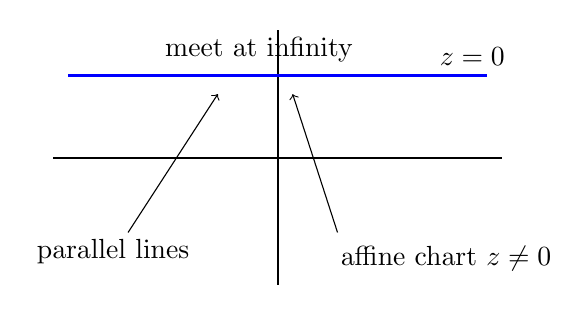
\begin{tikzpicture}[scale=0.95]
  \draw[thick] (-3,0) -- (3,0);
  \draw[thick] (0,-1.7) -- (0,1.7);
  \draw[very thick,blue] (-2.8,1.1) -- (2.8,1.1);
  \node at (2.6,1.35) {$z=0$};
  \node at (2.25,-1.35) {affine chart $z\ne0$};
  \draw[->] (-2,-1) -- (-.8,.85);
  \draw[->] (.8,-1) -- (.2,.85);
  \node at (-2.2,-1.25) {parallel lines};
  \node at (-.25,1.45) {meet at infinity};
\end{tikzpicture}
\end{center}

The diagram is deliberately schematic. The line at infinity is not physically above the plane; it is a projective completion of the affine picture.

\section{The cross-ratio as a first invariant}

Projective transformations do not preserve length, angle, or ordinary ratios of distances. But they do preserve one important quantity on a projective line: the cross-ratio.

For four points \(a,b,c,d\) on an affine coordinate line, define
\[
  [a,b;c,d]=\frac{(c-a)(d-b)}{(c-b)(d-a)}.
\]
This expression is unchanged under projective transformations of \(\mathbb P^1\).

The point of mentioning it here is not to develop a full theory of projective invariants. It is to show the change in taste: once distances are no longer meaningful, geometry searches for different invariants.

\section{Perspective as projective geometry}

A camera image is not an isometry of the world. It does not preserve lengths. But it sends straight lines to straight lines and preserves incidence. This is why projective geometry is the natural language of perspective.

Parallel railway tracks appear to meet at a vanishing point. In Euclidean geometry this is an illusion. In projective geometry it is exactly what the completed plane says should happen.


\section{What to remember}

Projective geometry is not harder because it adds infinity. It is easier because it removes exceptions.

\[
\begin{array}{c|c}
\text{affine habit} & \text{projective correction}\\
\hline
\text{parallel lines do not meet} & \text{they meet at infinity}\\
\text{coordinates are numbers} & \text{coordinates are ratios}\\
\text{line equations are separate from points} & \text{points and lines are dual}\\
\text{conics split into types} & \text{conics are one projective family}
\end{array}
\]

\include{tex/notes/N-20250211}


\part{Curves and Schemes}
\label{vol:13-curves-and-schemes}
\begingroup
\small
\sloppy
\parttoc
\endgroup

% This file is generated during volume reorganization.
% Volume: Curves and Schemes

\include{tex/notes/N-20220212}
\notechapter{N-20240608}{Plane Curves: Equations, Singularities, and Projective Closure}

\section{Curves as equations}

A plane algebraic curve is the zero set of a polynomial:
\[
  C=V(f)=\{(x,y)\in k^2:f(x,y)=0\}.
\]
This simple definition changes the meaning of geometry. A curve is no longer just a drawn shape; it is controlled by an algebraic equation.

\[
\begin{array}{c|c}
f(x,y) & \text{curve}\\
\hline
y-mx-b & \text{line}\\
x^2+y^2-1 & \text{circle}\\
y^2-x^3 & \text{cusp}\\
y^2-x^2(x+1) & \text{nodal cubic}
\end{array}
\]

\begin{figure}[H]
\centering
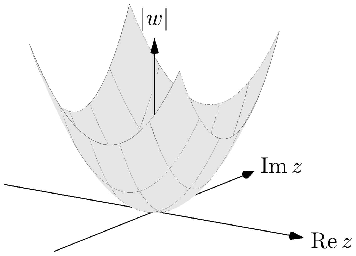
\includegraphics[width=.55\linewidth]{figures/N-20240608/parabola.pdf}
\caption{A familiar curve can be treated as an equation, not only as a picture.}
\end{figure}

\section{Coordinate rings}

The coordinate ring of \(C=V(f)\) is
\[
  k[C]=k[x,y]/(f).
\]
Two polynomials define the same function on the curve if they differ by a multiple of \(f\). So \(k[C]\) is the algebra of polynomial functions living on the curve.

This is one of the main ideas of algebraic geometry:
\[
  \text{study a space by studying its functions.}
\]

\section{Irreducibility}

If \(f=gh\), then
\[
  V(f)=V(g)\cup V(h).
\]
So factorization of polynomials corresponds to decomposition of curves.

For example, \(xy=0\) is the union of the two coordinate axes. It is reducible. A curve given by an irreducible polynomial is a single algebraic piece.

\section{Singular points}

A point \(p=(a,b)\in C\) is singular if
\[
  f(a,b)=0,\qquad f_x(a,b)=0,\qquad f_y(a,b)=0.
\]
At such a point, the usual tangent line is not well-defined by the linear approximation because the linear part vanishes.

For the cusp \(y^2=x^3\), the origin is singular. For the node \(y^2=x^2(x+1)\), the origin is also singular, but the local shape is different. A cusp has one branch with a sharp turn; a node has two branches crossing.

\section{Tangent cones}

If the lowest-degree nonzero part of \(f\) at a point is \(f_d\), then \(f_d=0\) describes the tangent cone. For a smooth point, this is just one tangent line. For a node, it can be two lines.

Example:
\[
  f(x,y)=y^2-x^2-x^3.
\]
The lowest-degree part is
\[
  y^2-x^2=(y-x)(y+x),
\]
so the tangent cone at the origin consists of the two lines \(y=x\) and \(y=-x\).

\section{Projective closure}

Affine curves can hide points at infinity. To see the whole curve, homogenize the equation. If
\[
  f(x,y)=y-x^2,
\]
then the homogenized equation is
\[
  F(x,y,z)=yz-x^2.
\]
The projective closure is \(V(F)\subset\mathbb P^2\). In the chart \(z=1\), we recover the original parabola. On the line at infinity \(z=0\), we get \(-x^2=0\), so \(x=0\), giving the point \([0:1:0]\).

Projective closure is the operation of filling in the missing directions at infinity.

\section{Bezout as a guiding principle}

A first form of Bezout's theorem says that two projective plane curves of degrees \(m\) and \(n\) meet in \(mn\) points, counted with multiplicity, over an algebraically closed field, provided they have no common component.

Its meaning is that projective geometry restores the correct accounting. Missing intersections at infinity and tangencies are not exceptions; they are counted correctly once the setting is projective and multiplicities are included.

%% expanded-on-review

\section{A coordinate-ring computation}

For the cusp
\[
  C=V(y^2-x^3),
\]
the coordinate ring is
\[
  k[C]=k[x,y]/(y^2-x^3).
\]
A useful parametrization is
\[
  x=t^2,\qquad y=t^3.
\]
This gives a map
\[
  k[x,y]/(y^2-x^3)\longrightarrow k[t],
  \qquad x\mapsto t^2,\quad y\mapsto t^3.
\]
The image is \(k[t^2,t^3]\), not all of \(k[t]\). This algebraic fact remembers the cusp: near the origin the curve is not as smooth as a line.

For the parabola \(y=x^2\), by contrast, the coordinate ring is just \(k[x]\). Algebraically it behaves like a line. This comparison is a good way to feel what singularities do: they make the function ring less simple.

\section{Intersection multiplicity by example}

Consider the line \(y=0\) and the parabola \(y=x^2\). They meet at the origin. Substituting \(y=0\) into \(y=x^2\) gives
\[
  x^2=0.
\]
So the intersection has multiplicity \(2\). Geometrically, the line is tangent to the parabola.

This small example explains why Bezout counts multiplicity. If one only counts visible points, a tangent intersection looks like one point. Algebra sees that the contact is doubled.

\section{Why projective closure changes counting}

The affine lines \(y=0\) and \(y=1\) do not meet in \(\mathbb A^2\). After homogenizing, they become
\[
  y=0,\qquad y-z=0.
\]
In \(\mathbb P^2\), they meet at \([1:0:0]\). Thus projective closure does not add decorative points; it repairs the accounting of intersections.

This is the same philosophy as projective geometry in the previous note, now applied to polynomial curves.


\section{What to remember}

Plane curves sit at the meeting point of algebra and geometry:
\[
\begin{array}{c|c}
\text{geometry} & \text{algebra}\\
\hline
\text{curve} & \text{polynomial equation}\\
\text{functions on the curve} & \text{coordinate ring}\\
\text{decomposition} & \text{factorization}\\
\text{singular point} & f=f_x=f_y=0\\
\text{points at infinity} & \text{homogenization}
\end{array}
\]

\notechapter{N-20240914}{Divisors on Curves: Zeros, Poles, and the Shape of Meromorphic Functions}

\section{Why count zeros and poles}

On a Riemann surface, a meromorphic function can have zeros and poles. Instead of listing them informally, we package them into a divisor.

A divisor is a finite formal sum
\[
  D=\sum_p n_p[p],
\]
where \(n_p\in\mathbb Z\) and only finitely many \(n_p\) are nonzero. Positive coefficients record zeros; negative coefficients record poles.

\section{Principal divisors}

For a nonzero meromorphic function \(f\), define its principal divisor by
\[
  (f)=\sum_p \operatorname{ord}_p(f)[p].
\]
This records all zeros and poles of \(f\), with multiplicity.

On the Riemann sphere, the rational function
\[
  f(z)=\frac{(z-a)^2}{z-b}
\]
has divisor
\[
  (f)=2[a]-[b]-[\infty],
\]
because the total degree of a principal divisor on a compact Riemann surface is zero.

\section{Degree}

The degree of a divisor is
\[
  \deg D=\sum_p n_p.
\]
For a principal divisor on a compact Riemann surface,
\[
  \deg(f)=0.
\]
This says that zeros and poles balance.

\section{Divisors as permissions}

A divisor \(D\) can be read as a rule for allowed poles and required zeros. Define
\[
  L(D)=\{f\text{ meromorphic}: (f)+D\ge0\}\cup\{0\}.
\]
If \(D\) is positive, it allows poles bounded by \(D\).

On \(\mathbb{CP}^1\), the space \(L(n[\infty])\) consists of polynomials of degree at most \(n\):
\[
  L(n[\infty])=\{a_0+a_1z+\cdots+a_nz^n\}.
\]
So \(\ell(n[\infty])=n+1\).

\section{Line bundles without panic}

A line bundle is a family of one-dimensional vector spaces varying over a curve. Locally it looks like \(U\times\mathbb C\), but globally the local pieces may be glued with nontrivial transition functions.

Divisors produce line bundles. The line bundle \(\mathcal O(D)\) is designed so that its sections are meromorphic functions obeying the permission rule encoded by \(D\).

This is why divisors are not merely bookkeeping. They control spaces of functions and sections.

\section{The canonical divisor}

Holomorphic \(1\)-forms also have zeros. Their divisor class is called the canonical divisor \(K\). It measures the intrinsic differential geometry of the curve.

For a compact Riemann surface of genus \(g\),
\[
  \deg K=2g-2.
\]
This number already remembers the topology of the surface.

\begin{figure}[H]
\centering
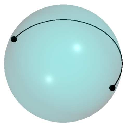
\includegraphics[width=.42\linewidth]{figures/N-20240914/1cycle.pdf}
\caption{A curve carries both topology and analytic data. Divisors are one way to connect them.}
\end{figure}

\section{Riemann--Roch as a counting theorem}

The Riemann--Roch theorem says
\[
  \ell(D)-\ell(K-D)=\deg D+1-g.
\]
This formula should not be read first as a technical spell. It is a counting theorem: it tells us how many meromorphic functions are allowed by a divisor, corrected by topology and differential forms.

For \(X=\mathbb{CP}^1\), \(g=0\), and \(D=n[\infty]\), it gives \(\ell(D)=n+1\), matching polynomials of degree at most \(n\).

\section{Hurwitz in one paragraph}

If \(f:X\to Y\) is a nonconstant holomorphic map of compact Riemann surfaces of degree \(d\), the Hurwitz formula is
\[
  2g_X-2=d(2g_Y-2)+\sum_{p\in X}(e_p-1).
\]
The integer \(e_p\) is the ramification index at \(p\). The formula says that topology changes under covering maps exactly by the ramification correction.

%% expanded-on-review

\section{Three examples on the Riemann sphere}

On \(\mathbb{CP}^1\), the function \(z-a\) has one zero at \(a\) and one pole at \(\infty\):
\[
  (z-a)=[a]-[\infty].
\]
The function \(1/(z-a)\) has divisor
\[
  \left(\frac1{z-a}\right)=-[a]+[\infty].
\]
The function \((z-a)/(z-b)\) has divisor
\[
  \left(\frac{z-a}{z-b}\right)=[a]-[b].
\]
These examples are small, but they show the whole idea: a divisor records the balance sheet of zeros and poles.

\section{Riemann--Roch on the Projective Line}

Let \(D=n[\infty]\). The condition \((f)+D\ge0\) says that \(f\) may have a pole at infinity of order at most \(n\), and no other poles. Such functions are exactly polynomials of degree at most \(n\):
\[
  1,z,z^2,\ldots,z^n.
\]
So
\[
  \ell(D)=n+1.
\]
Since \(g=0\), Riemann--Roch predicts
\[
  \ell(D)-\ell(K-D)=n+1.
\]
For \(n\ge0\), the correction term \(\ell(K-D)\) vanishes, and the formula becomes the elementary dimension count above.

This is the right way to first meet Riemann--Roch: on the sphere it says something one can already verify by hand.

\section{What not to overread}

Divisors are not a replacement for geometry. They are a language for one kind of geometric question: which functions or sections can exist with prescribed zeros and poles?

The danger is to memorize the notation while forgetting the picture. Whenever \(D\) appears, ask what behavior it permits. Whenever \(L(D)\) appears, ask which functions survive those permissions.


\section{What to remember}

Divisors turn zeros and poles into algebra. Line bundles turn divisor conditions into spaces of sections. Riemann--Roch tells us how large those spaces are.

\[
  \text{geometry asks which functions exist, and divisors say what behavior is allowed.}
\]

\notechapter{N-20241026}{Zariski Geometry: Varieties, Coordinate Rings, and Sheaves Without Fear}

\section{The algebra-geometry dictionary}

Affine algebraic geometry begins with polynomial equations. Given an ideal
\[
  I\subset k[x_1,\ldots,x_n],
\]
its zero set is
\[
  V(I)=\{a\in k^n:f(a)=0\text{ for all }f\in I\}.
\]
Conversely, for a set \(X\subset k^n\), the ideal of functions vanishing on it is
\[
  I(X)=\{f:f(x)=0\text{ for all }x\in X\}.
\]

\[
\begin{array}{c|c}
\text{geometry} & \text{algebra}\\
\hline
\text{affine variety} & \text{radical ideal}\\
\text{irreducible variety} & \text{prime ideal}\\
\text{regular functions} & \text{coordinate ring}\\
\text{local behavior} & \text{localization / stalks}
\end{array}
\]

\section{Coordinate rings}

If \(X=V(I)\), its coordinate ring is
\[
  k[X]=k[x_1,\ldots,x_n]/I(X).
\]
This is the ring of polynomial functions on \(X\).

Example: for the parabola \(X=V(y-x^2)\),
\[
  k[X]=k[x,y]/(y-x^2)\cong k[x].
\]
The parabola is algebraically the same as a line, even though it is drawn curved in the plane.

\section{Nullstellensatz as a promise}

Over an algebraically closed field, Hilbert's Nullstellensatz says that ideals and algebraic sets match after taking radicals:
\[
  I(V(I))=\sqrt I.
\]
This tells us that the algebra of polynomial equations remembers the geometry of their common zero set, up to nilpotent information.

\[
  \text{radical ideals are the algebraic shadows of affine varieties.}
\]

\section{The Zariski topology}

Closed sets in the Zariski topology are algebraic sets. This topology is much coarser than the usual Euclidean topology. For example, in \(\mathbb A^1\), proper closed sets are finite sets.

This feels strange at first. But the Zariski topology is designed so that polynomial functions behave naturally. It is not meant to measure physical closeness; it measures algebraic dependence.

\begin{figure}[H]
\centering
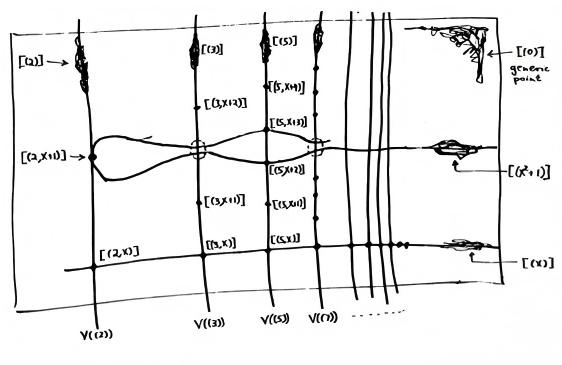
\includegraphics[width=.45\linewidth]{figures/N-20241026/mumforddrawing.jpg}
\caption{A useful mental picture: algebraic geometry keeps functions, equations, and shapes tied together.}
\end{figure}

\section{Regular functions are local}

On affine space, polynomial functions are regular. On more general open subsets, regular functions may look like fractions
\[
  \frac{f}{g},
\]
where \(g\) does not vanish on the open set being considered.

This locality is crucial. Geometry is not only about global polynomial formulas; it is about functions that are locally polynomial fractions.

\section{Why sheaves appear}

A sheaf is a device for keeping track of local data and gluing it when the local pieces agree. For regular functions, the sheaf condition says:
\[
\begin{array}{c}
  \text{if functions are defined locally,}\\
  \text{and they agree on overlaps,}\\
  \text{then they glue to a unique global function.}
\end{array}
\]
This is not abstract decoration. It is exactly what one expects of functions on a space.

\section{Stalks and germs}

The stalk of a sheaf at a point \(p\) stores the local behavior near \(p\). For regular functions, elements of the stalk are germs: two functions define the same germ if they agree on some neighborhood of \(p\).

The stalk is the algebraic microscope of the variety. It ignores what happens far away and keeps what can be seen arbitrarily close to the point.

%% expanded-on-review

\section{Distinguished opens by example}

In \(\mathbb A^1=\operatorname{Spec}k[x]\), the open set
\[
  D(x)=\{\text{points where }x\ne0\}
\]
corresponds to allowing \(x\) in denominators. The regular functions on this open set are Laurent polynomials
\[
  k[x,x^{-1}].
\]
This is the simplest example of localization.

In \(\mathbb A^2\), the open set \(D(x)\) removes the \(y\)-axis. On it, \(1/x\) is a perfectly regular function. This is why regular functions cannot be understood only as global polynomials on the whole ambient space.

\section{Sheaf gluing in a familiar case}

Cover a space by two open sets \(U\) and \(V\). Suppose we have a regular function \(f_U\) on \(U\) and a regular function \(f_V\) on \(V\). If
\[
  f_U|_{U\cap V}=f_V|_{U\cap V},
\]
then the sheaf condition says there is a unique function \(f\) on \(U\cup V\) restricting to both.

This may sound obvious for ordinary functions. That is precisely why it is the correct abstraction. Sheaves formalize the ordinary behavior of local data.

\section{A warning about pictures}

The Zariski topology is too coarse to be drawn faithfully. A line with the Zariski topology is not like a line with the Euclidean topology. Removing finitely many points still leaves a large open set.

So pictures in algebraic geometry should be treated as memory aids, not literal topology. The reliable object is the dictionary between equations, ideals, rings, and local functions.



\section{One more example: the hyperbola}

Let
\[
  X=V(xy-1)\subset\mathbb A^2.
\]
Its coordinate ring is
\[
  k[X]=k[x,y]/(xy-1).
\]
Since \(xy=1\), the element \(x\) is invertible and \(y=x^{-1}\). Hence
\[
  k[X]\cong k[x,x^{-1}].
\]
So the hyperbola is algebraically the affine line with the origin removed. This example is a good reminder that coordinate rings often reveal a simpler shape than the drawing suggests.


\section{What to remember}

Zariski geometry is not ordinary geometry with a weird topology. It is geometry rebuilt around polynomial functions.

\[
\begin{array}{c}
  \text{equations define spaces,}\\
  \text{functions on spaces form rings,}\\
  \text{local functions form sheaves,}\\
  \text{stalks record what happens near a point.}
\end{array}
\]

\notechapter{N-20250118}{Schemes Gently: Prime Ideals as Points and Functions as Local Data}

\section{Why schemes appear}

Affine varieties are built from polynomial equations over algebraically closed fields. Schemes enlarge this world. They allow arithmetic examples, nilpotents, and spaces that are glued from affine pieces.

The first definition is surprisingly short:
\[
  \operatorname{Spec}R=\{\mathfrak p\subset R:\mathfrak p\text{ is a prime ideal}\}.
\]
A scheme begins by treating prime ideals as points.

\section{Prime ideals as generalized points}

For \(R=k[x]\), maximal ideals \((x-a)\) correspond to ordinary points \(a\in k\). But \((0)\) is also a prime ideal. It is a generic point: it is not one location, but the whole irreducible line viewed algebraically.

Thus \(\operatorname{Spec}R\) contains more than classical points. It contains information about irreducible pieces and specialization.

\section{Closed sets and opens}

For an ideal \(I\subset R\), define
\[
  V(I)=\{\mathfrak p\in\operatorname{Spec}R:I\subseteq\mathfrak p\}.
\]
These sets are closed in the Zariski topology.

The distinguished open set associated to \(f\in R\) is
\[
  D(f)=\{\mathfrak p:f\notin\mathfrak p\}.
\]
One should read \(D(f)\) as the region where \(f\) is allowed to be inverted.

\section{Examples}

For a field \(k\), \(\operatorname{Spec}k\) has one point.

For \(k[x]\), \(\operatorname{Spec}k[x]\) contains closed points \((x-a)\) and the generic point \((0)\).

For \(\mathbb Z\), \(\operatorname{Spec}\mathbb Z\) has points \((p)\) for each prime number \(p\), together with the generic point \((0)\). This is why people say \(\operatorname{Spec}\mathbb Z\) behaves like an arithmetic curve.

\section{Nilpotents and the double point}

Consider
\[
  R=k[x]/(x^2).
\]
The element \(x\) is nonzero but nilpotent:
\[
  x^2=0.
\]
The topological space \(\operatorname{Spec}R\) has only one point, but the ring remembers an infinitesimal thickening at that point.

This is one of the main reasons schemes are useful. They do not throw away nilpotent information.

\section{The structure sheaf}

A space is not enough. We also need functions on it. On a distinguished open \(D(f)\), the functions are given by localization:
\[
  \mathcal O_{\operatorname{Spec}R}(D(f))=R_f.
\]
Here \(R_f\) means that powers of \(f\) are allowed in denominators.

This formula is the computational heart of affine schemes.

\section{Stalks and local rings}

At a prime ideal \(\mathfrak p\), the stalk of the structure sheaf is
\[
  \mathcal O_{\operatorname{Spec}R,\mathfrak p}=R_{\mathfrak p}.
\]
This is a local ring. It focuses on functions near the point \(\mathfrak p\) by inverting elements not in \(\mathfrak p\).

The local ring is the algebraic version of a small neighborhood.

\section{A safe mental model}

A scheme is not just a set of prime ideals. It is a space with a sheaf of rings. The points tell us where we are; the rings tell us what functions are available near each point.

\[
\begin{array}{c|c}
\text{scheme idea} & \text{meaning}\\
\hline
\operatorname{Spec}R & \text{prime ideals as points}\\
V(I) & \text{closed condition}\\
D(f) & \text{place where }f\text{ is invertible}\\
R_f & \text{functions on }D(f)\\
R_{\mathfrak p} & \text{functions near }\mathfrak p
\end{array}
\]

%% expanded-on-review

\section{The topology of the affine line spectrum}

The space \(\operatorname{Spec}k[x]\) has a generic point \((0)\) and closed points \((x-a)\). The closure of the generic point is the whole space:
\[
  \overline{\{(0)\}}=\operatorname{Spec}k[x].
\]
The closure of \((x-a)\) is just itself.

This is very different from ordinary Hausdorff geometry. But it is meaningful: the generic point represents the whole irreducible line, while a closed point represents a particular value of \(x\).

\begin{center}
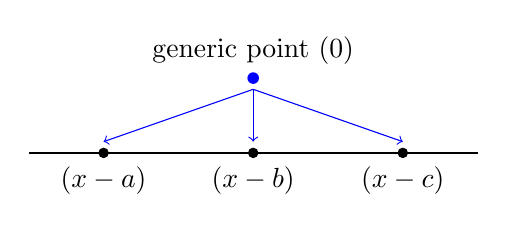
\begin{tikzpicture}[scale=0.95]
  \draw[thick] (-3,0) -- (3,0);
  \foreach \x/\lab in {-2/{(x-a)},0/{(x-b)},2/{(x-c)}} {
    \fill (\x,0) circle (2pt);
    \node[below] at (\x,-.05) {$\lab$};
  }
  \fill[blue] (0,1.0) circle (2.2pt);
  \node[above] at (0,1.05) {generic point $(0)$};
  \draw[->,blue] (0,.85) -- (-2,.15);
  \draw[->,blue] (0,.85) -- (0,.15);
  \draw[->,blue] (0,.85) -- (2,.15);
\end{tikzpicture}
\end{center}

The arrows are only suggestive: the generic point specializes to closed points.

\section{Localization as zooming in}

For a prime ideal \(\mathfrak p\), the local ring
\[
  R_{\mathfrak p}
\]
is obtained by inverting everything not in \(\mathfrak p\). This means that near \(\mathfrak p\), functions not vanishing there are treated as units.

For \(R=k[x]\) and \(\mathfrak p=(x-a)\), the local ring
\[
  k[x]_{(x-a)}
\]
contains rational functions whose denominators do not vanish at \(a\). This is exactly the algebraic version of functions defined near \(a\).

\section{Why nilpotents are geometric}

The ring \(k[x]/(x^2)\) has the same classical point as \(k[x]/(x)\), but it has more infinitesimal information. The element \(x\) is not zero, yet its square is zero.

A useful mental picture is that \(\operatorname{Spec}k[x]/(x^2)\) is a point with a first-order tangent fuzz. The point cannot be separated into two visible points, but algebra can still detect a direction of infinitesimal thickening.



\section{Why the spectrum of the integers is geometric}

The points \((p)\) of \(\operatorname{Spec}\mathbb Z\) behave like closed points, one for each prime number. The point \((0)\) behaves like a generic point. An integer \(n\) vanishes at exactly the prime ideals \((p)\) with \(p\mid n\).

Thus divisibility becomes geometry:
\[
  V(n)=\{(p):p\mid n\}.
\]
This is one of the most charming reasons schemes are worth learning: arithmetic starts to look like a geometric space.


\section{What to remember}

Schemes are a controlled generalization of algebraic varieties. They keep ordinary points, generic points, arithmetic points, and infinitesimal information in one language.

The main idea is not to make geometry obscure. It is to let algebraic geometry keep the information that classical point sets forget.

\notechapter{N-20250301}{Projective Schemes and Gluing: A Gentle View of Proj}

\section{Why projective schemes are needed}

Projective varieties are built from homogeneous equations. Schemes ask for the same idea at the level of rings, prime ideals, and local functions.

The construction is called \(\operatorname{Proj}\). It is the projective companion of \(\operatorname{Spec}\).

If \(S\) is a graded ring
\[
  S=S_0\oplus S_1\oplus S_2\oplus\cdots,
\]
then \(\operatorname{Proj}S\) is built from homogeneous prime ideals not containing the irrelevant ideal.

This sounds technical, but the basic idea is familiar: projective geometry ignores common scaling, so only homogeneous data make sense.

\section{Projective space}

The most important example is
\[
  \mathbb P^n_R=\operatorname{Proj}R[x_0,\ldots,x_n],
\]
where the variables have degree \(1\).

The standard affine chart \(x_i\ne0\) is written
\[
  D_+(x_i).
\]
On this chart, ratios
\[
  \frac{x_j}{x_i}
\]
become ordinary affine coordinates.

So projective space is assembled from affine pieces, one for each coordinate that is nonzero.

\section{Homogeneous ideals}

A projective subscheme of \(\mathbb P^n\) is described by a homogeneous ideal
\[
  I\subset R[x_0,\ldots,x_n].
\]
Homogeneous equations are necessary because the point
\[
  [x_0:\cdots:x_n]
\]
is unchanged by scaling all coordinates.

For example, a projective conic is given by a homogeneous quadratic equation
\[
  F(x,y,z)=0.
\]
In the chart \(z\ne0\), it becomes an affine equation in \(x/z\) and \(y/z\).

\section{Gluing affine charts}

The most concrete way to think about \(\operatorname{Proj}\) is gluing. Each \(D_+(x_i)\) is affine. The overlaps \(D_+(x_i)\cap D_+(x_j)\) are also affine, and the coordinate changes are given by ratios.

For \(\mathbb P^1\), there are two charts:
\[
  U_0=\{x_0\ne0\},\qquad U_1=\{x_1\ne0\}.
\]
On \(U_0\), use coordinate \(t=x_1/x_0\). On \(U_1\), use coordinate \(s=x_0/x_1\). On the overlap,
\[
  s=\frac1t.
\]
This is the same gluing pattern as the Riemann sphere.

\section{Projective closure revisited}

Given an affine equation \(f(x,y)=0\), homogenizing it gives a projective equation
\[
  F(x,y,z)=0.
\]
The projective scheme remembers not only the affine curve but also what happens at infinity and, if present, nilpotent or embedded structure.

This is a scheme-level version of a familiar geometric act: complete the affine picture by adding the missing directions at infinity.

\section{Why this is not too abstract}

The point of \(\operatorname{Proj}\) is not to make projective geometry harder. It lets projective geometry use the same local-function language as \(\operatorname{Spec}\).

The repeated pattern is:
\[
\begin{array}{c}
  \text{build local affine pieces,}\\
  \text{understand their rings of functions,}\\
  \text{glue them along overlaps.}
\end{array}
\]

\section{Relation with the earlier conic note}

The earlier Erlangen-style conic note emphasized transformations and invariants. The scheme viewpoint emphasizes functions and local rings. These are not competing views.

\[
\begin{array}{c|c}
\text{projective geometry} & \text{incidence, duality, transformations}\\
\text{algebraic geometry} & \text{equations, coordinate rings, local functions}\\
\text{scheme theory} & \text{nilpotents, gluing, base rings}
\end{array}
\]

The same shape becomes richer as the language becomes richer.

%% expanded-on-review

\section{The two-chart construction of the projective line}

The most useful model of \(\operatorname{Proj}\) is still the elementary construction of \(\mathbb P^1\). Take two affine lines:
\[
  U_0=\operatorname{Spec}R[t],\qquad U_1=\operatorname{Spec}R[s].
\]
On the open subsets where \(t\ne0\) and \(s\ne0\), glue by
\[
  s=\frac1t.
\]
The result is projective line.

This example should be kept in mind whenever \(\operatorname{Proj}\) feels abstract. The construction is not a single mysterious space; it is affine geometry plus gluing rules.

\section{Standard opens in the projective plane}

Projective plane has three standard affine charts:
\[
  D_+(x),\qquad D_+(y),\qquad D_+(z).
\]
On \(D_+(z)\), the affine coordinates are
\[
  X=\frac{x}{z},\qquad Y=\frac{y}{z}.
\]
On \(D_+(x)\), one uses
\[
  U=\frac{y}{x},\qquad V=\frac{z}{x}.
\]
The projective plane is what appears after gluing these charts along their overlaps.

This makes projective geometry feel less like adding a mystical line at infinity and more like coordinating several affine windows.

\section{A conic across charts}

The projective conic
\[
  xz-y^2=0
\]
looks different in different charts. On \(z\ne0\), it becomes
\[
  X=Y^2.
\]
On \(x\ne0\), it becomes
\[
  V=U^2.
\]
The same projective curve has multiple affine faces. A single affine picture can hide part of the curve, especially at infinity.

\section{What Proj adds to the earlier story}

The earlier projective note explained homogeneous coordinates and incidence. This note adds the function-theoretic layer:
\[
\begin{array}{c|c}
\text{homogeneous coordinates} & \text{homogeneous primes}\\
\text{affine charts} & \text{standard affine opens}\\
\text{projective equations} & \text{homogeneous ideals}
\end{array}
\]
The new language is heavier, but the basic picture is the same: projective spaces are made by gluing affine charts.


\section{What to remember}

\(\operatorname{Spec}\) turns rings into affine geometric spaces. \(\operatorname{Proj}\) turns graded rings into projective geometric spaces.

\[
  \text{Proj is projective geometry rebuilt from homogeneous algebra and affine gluing.}
\]
This is a good endpoint for the Geometry volume: it returns to projective geometry, but now with the function-theoretic language of schemes.



\part{Topology and Homotopy}
\label{vol:14-topology-and-homotopy}
\begingroup
\small
\sloppy
\parttoc
\endgroup

\input{tex/volumes/vol-14-topology-and-homotopy}

\part{Geometric Structures and Knots}
\label{vol:15-geometric-structures-and-knots}
\begingroup
\small
\sloppy
\parttoc
\endgroup

% This file is generated during volume reorganization.
% Volume: Geometric Structures and Knots

\notechapter{N-20221214}{Tarski's Circle-Squaring Problem: From Polygon Dissection to Borel Equidecomposition}

\section{The route of the note}

This note is about Tarski's circle-squaring problem, but the source pages do not treat it as a single isolated puzzle.  They move through a sequence of increasingly subtle notions:
\[
\begin{gathered}
  \text{Tarski circle-squaring}\longrightarrow \text{Hilbert's third problem}\\
  \longrightarrow \text{measure and paradoxical decomposition}\\
  \longrightarrow \text{Laczkovich's theorem}\longrightarrow \text{Borel circle squaring}.
\end{gathered}
\]
The figures below are kept only when the visual configuration itself matters.  The surrounding theorem statements, comments, formulas, and handwritten annotations have been incorporated into the prose.

Tarski asked in 1925 whether a disk and a square of equal area in the plane are equidecomposable: can the disk be partitioned into finitely many pieces, and can those pieces be moved by isometries to partition the square?

\section{Equidecomposability and dissection congruence}

Let a group $G$ act on a set $X$.  Two subsets $A,B\subseteq X$ are $G$-equidecomposable if there are finite partitions
\[
  A=A_1\sqcup\cdots\sqcup A_m,
  \qquad
  B=B_1\sqcup\cdots\sqcup B_m,
\]
and elements $g_i\in G$ such that
\[
  g_i(A_i)=B_i.
\]
For plane polygons, one usually lets $G$ be the group of Euclidean isometries.  In that setting the classical language is dissection congruence: cut one polygon into finitely many polygonal pieces and rearrange them to obtain the other.

The first example is the familiar parallelogram-to-rectangle cut.

\begin{figure}[H]
\centering
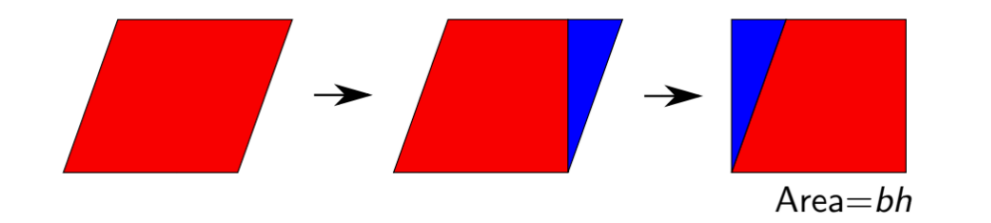
\includegraphics[width=.66\linewidth]{figures/N-20221214/01-parallelogram-to-rectangle.png}
\caption{A parallelogram dissected and rearranged into a rectangle.}
\end{figure}

Area is obviously preserved by dissection congruence.  The Wallace--Bolyai--Gerwien theorem says that, for plane polygons, area is also sufficient.

\begin{theorem}[Wallace--Bolyai--Gerwien]
Any two plane polygons of the same area are dissection congruent.
\end{theorem}

One small point in the note is transitivity.  If polygon $P$ is dissection congruent to $Q$, and $Q$ is dissection congruent to $R$, then $P$ is dissection congruent to $R$.  One refines the two dissections so that the intermediate polygon $Q$ is cut compatibly, then composes the rearrangements.

\begin{figure}[H]
\centering
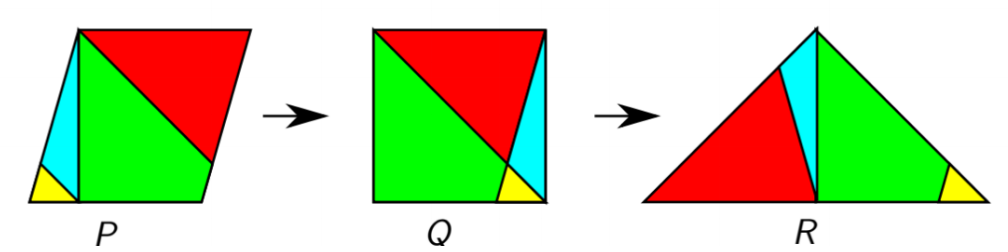
\includegraphics[width=.72\linewidth]{figures/N-20221214/02-polygon-transitivity-PQR.png}
\caption{The transitivity intuition: a dissection from $P$ to $Q$ and one from $Q$ to $R$ compose.}
\end{figure}

The proof of the theorem is constructive.  First chop a polygon into triangles.

\begin{figure}[H]
\centering
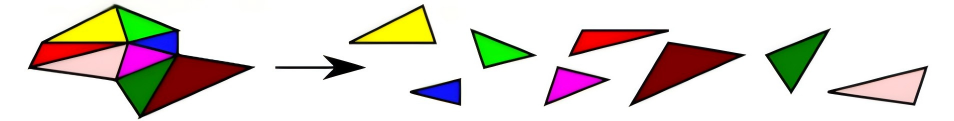
\includegraphics[width=.76\linewidth]{figures/N-20221214/03-polygon-triangulation.png}
\caption{The first reduction: chop a polygon into triangles.}
\end{figure}

Then dissect each triangle into a parallelogram and then a rectangle; dissect each rectangle into a square; combine squares by the Pythagorean dissection.

\begin{figure}[H]
\centering
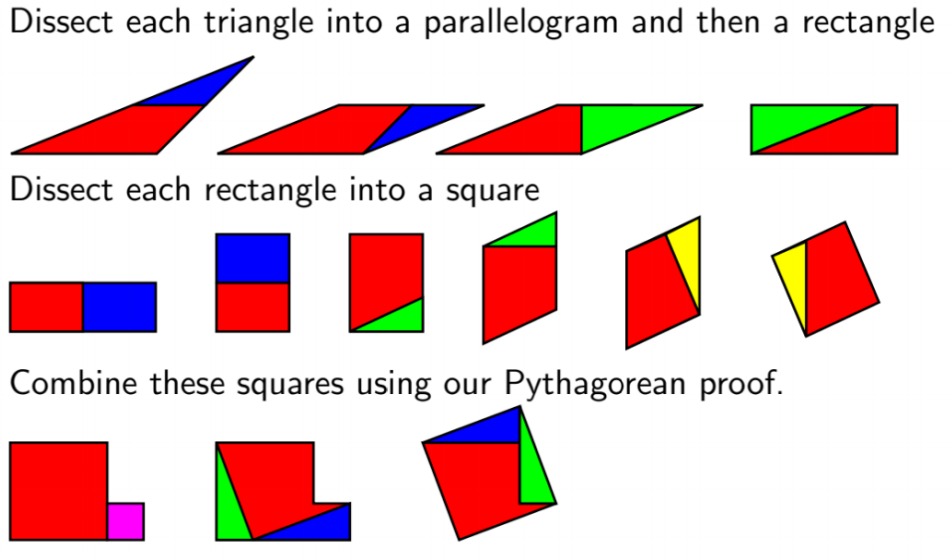
\includegraphics[width=.75\linewidth]{figures/N-20221214/04-triangle-rectangle-square-chain.png}
\caption{The visual chain: triangle to parallelogram/rectangle, rectangles to squares, then combine squares.}
\end{figure}

The theorem establishes the baseline: for tame plane polygons, equal area exactly characterizes finite dissection congruence.

\section{Hilbert's third problem and the Dehn invariant}

Hilbert's third problem asks whether equal volume similarly characterizes dissection congruence of three-dimensional polytopes.  Dehn's theorem says no: a cube and a regular tetrahedron of the same volume are not dissection congruent.

The extra obstruction is the Dehn invariant.  If a polyhedron has edge lengths $\ell_i$ and corresponding dihedral angles $\theta_i$, the invariant has the form
\[
  D(P)=\sum_i \ell_i\otimes \theta_i
\]
with values in a tensor product such as $\mathbb R\otimes_{\mathbb Z} \mathbb R/(2\pi\mathbb Z)$, depending on conventions.  The invariant records length-angle data that volume does not see.  The handwritten note correctly marks the tensor product as a point worth noticing: this is not elementary area bookkeeping anymore.

Sydler's theorem says that volume and Dehn invariant together are complete in dimension three.  Thus the two-dimensional polygon theorem has no naive three-dimensional analogue.

\section{Measure-theoretic background}

The source page then discusses measure.  Vitali sets imply that for every $n\ge1$, there is no extension of Lebesgue measure to all subsets of $\mathbb R^n$ that is both countably additive and invariant under isometries.

If countable additivity is weakened to finite additivity, the dimension matters.  For $n\ge3$, the Banach--Tarski paradox shows that there is no such finitely additive isometry-invariant measure on all bounded sets compatible with volume.  For $n\le2$, Banach measures exist.  The note emphasizes the reason: in dimension at least three, the isometry group contains enough free-group behavior to allow paradoxical decompositions; in dimensions one and two it does not.

For Tarski's problem in the plane, this means that equal area is still a necessary condition.  A disk and square that are equidecomposable by isometries must have the same Lebesgue measure, even if the pieces themselves are nonmeasurable.

\section{Tarski's circle-squaring problem}

The central question is then:

\begin{quote}
Are a disk and a square in $\mathbb R^2$ of the same area equidecomposable?
\end{quote}

\begin{figure}[H]
\centering
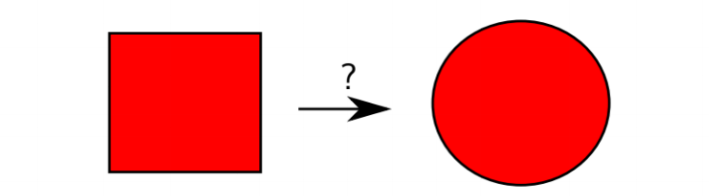
\includegraphics[width=.55\linewidth]{figures/N-20221214/05-disc-square-question.png}
\caption{The central visual question: equal-area disk and square.}
\end{figure}

At first sight the boundary seems to obstruct the construction.  A disk has circular boundary; a square has straight boundary.  This intuition is correct for a stricter notion, but not for arbitrary equidecomposition.

\section{Scissors congruence and why nice pieces fail}

The note distinguishes equidecomposability from scissors congruence.  In the scissors-congruence version, the pieces must be tame: each piece is homeomorphic to a disk and has boundary given by curves of finite length.  Under such restrictions, the disk and square are not scissors congruent.

The invariant mentioned in the source is:
\[
  \text{convex circular perimeter}-\text{concave circular perimeter}.
\]
When a curved circular arc is created inside a dissection, it is paired with an opposite concave arc, so the internal contributions cancel.  The remaining outer boundary contribution is preserved.  A disk has a nonzero circular-boundary contribution, while a square has none.  Hence a disk and square cannot be scissors congruent in this tame sense.

\begin{figure}[H]
\centering
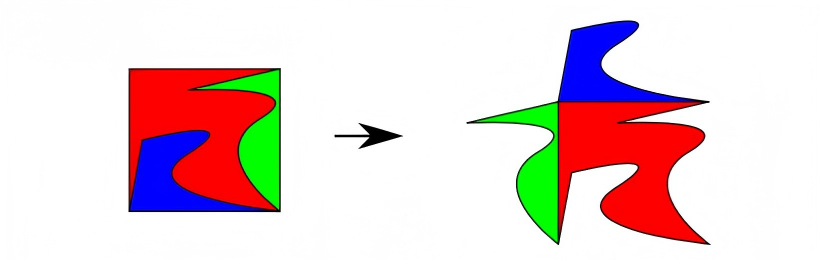
\includegraphics[width=.58\linewidth]{figures/N-20221214/06-scissors-congruence-pieces.png}
\caption{Tame scissors pieces preserve circular-boundary information.}
\end{figure}

This is the first major subtlety: the positive answer to Tarski's problem requires pieces much wilder than ordinary scissors pieces.

\section{Laczkovich's positive theorem}

Laczkovich proved in 1990 that Tarski's circle-squaring problem has a positive answer.  In 1992 he proved a broader theorem.  A simplified statement is:

\begin{theorem}[Laczkovich]
Let $A,B\subseteq \mathbb R^k$ be bounded sets with the same positive Lebesgue measure.  If the boundaries of $A$ and $B$ have upper Minkowski dimension strictly less than $k$, then $A$ and $B$ are equidecomposable by translations.
\end{theorem}

For a disk and square in the plane, the boundaries are one-dimensional, so the hypothesis applies.

The proof does not draw a literal jigsaw.  It converts the problem into a bounded matching problem in a graph generated by translations.

\section{First idea: work in the torus}

Scale and translate $A$ and $B$ so that they lie inside $[0,1)^k$.  Identify this cube with the $k$-torus
\[
  \mathbb T^k=(\mathbb R/\mathbb Z)^k.
\]
Then $A$ and $B$ are equidecomposable by translations as subsets of the torus iff, after possibly using more pieces, they are equidecomposable by translations in $\mathbb R^k$.

\begin{figure}[H]
\centering
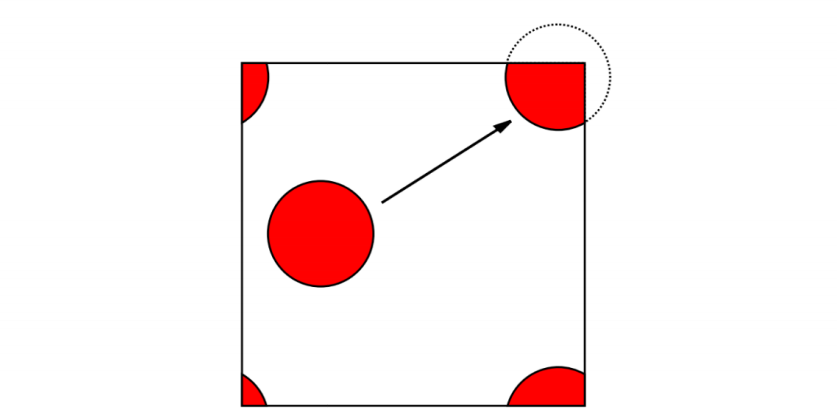
\includegraphics[width=.48\linewidth]{figures/N-20221214/07-torus-wraparound.png}
\caption{Working on the torus: translations wrap around the fundamental cube.}
\end{figure}

This torus reduction matters because translations become an action on a compact group.  Compactness and periodic boundary conditions make the orbit structure manageable.

\section{Random translations and a free action}

Choose a sufficiently large integer $d$ and random translations
\[
  u_1,\ldots,u_d\in\mathbb T^k.
\]
They define an action of $\mathbb Z^d$ on $\mathbb T^k$ by
\[
  (n_1,\ldots,n_d)\cdot x
  =n_1u_1+\cdots+n_du_d+x.
\]
For almost every choice of the $u_i$, this action is free: no nonzero element of $\mathbb Z^d$ fixes a point.  Thus each orbit can be visualized as a copy of $\mathbb Z^d$.

\begin{figure}[H]
\centering
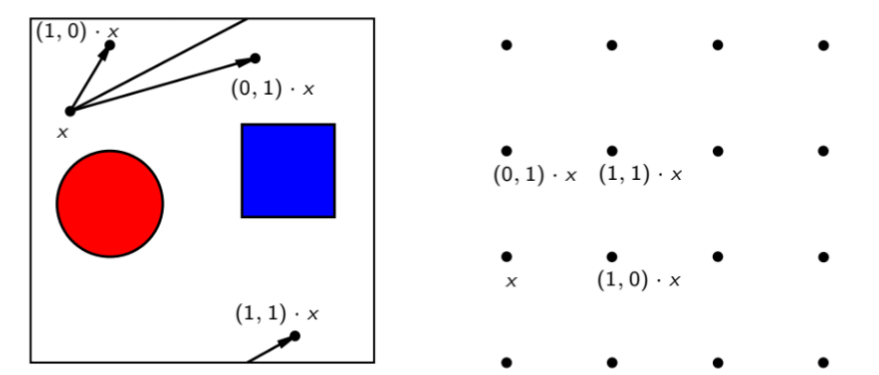
\includegraphics[width=.68\linewidth]{figures/N-20221214/08-random-translations.png}
\caption{Random translations generate lattice-like orbits on the torus.}
\end{figure}

\section{The graph and bounded-distance bijection}

Define a graph $G$ with vertex set $\mathbb T^k$.  Two points $x,y$ are adjacent if there exists $g\in\mathbb Z^d$ with
\[
  g\cdot x=y,
  \qquad
  \|g\|_\infty=1.
\]
So edges correspond to single generator moves.

\begin{figure}[H]
\centering
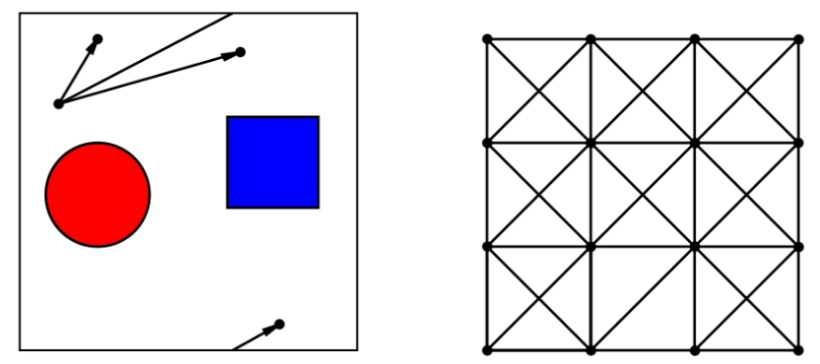
\includegraphics[width=.64\linewidth]{figures/N-20221214/09-graph-generator-grid.png}
\caption{The generator graph: locally it looks like a lattice with bounded moves.}
\end{figure}

To show $A$ and $B$ are equidecomposable, it suffices to find a Borel bijection
\[
  f:A\to B
\]
of bounded distance in $G$: there is some fixed $N$ such that
\[
  d_G(x,f(x))\le N
  \qquad \text{for all }x\in A.
\]
If such an $f$ exists, then only finitely many group elements $g$ can occur.  Put
\[
  A_g=\{x\in A:f(x)=g\cdot x\}.
\]
The sets $A_g$ partition $A$, and the translated sets $g\cdot A_g$ partition $B$.  This gives the desired finite equidecomposition.

This is the conceptual heart of the proof:
\[
  \text{finite translation equidecomposition}
  \quad\Longleftarrow\quad
  \text{bounded-distance orbit matching}.
\]

\section{Orbit matching}

Inside a single orbit of the $\mathbb Z^d$ action, the problem becomes matching red $A$-points to blue $B$-points by bounded paths.

\begin{figure}[H]
\centering
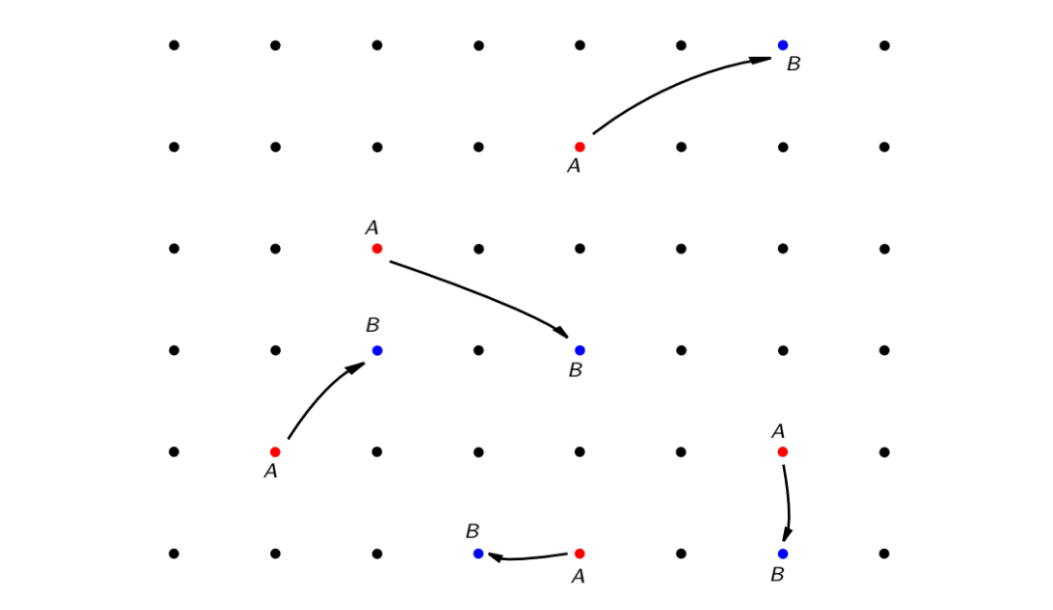
\includegraphics[width=.66\linewidth]{figures/N-20221214/10-orbit-matching.png}
\caption{Within one orbit, equidecomposition becomes a matching problem.}
\end{figure}

A bounded matching can exist only if large finite regions of the orbit contain approximately the same number of $A$-points and $B$-points.  This leads to discrepancy estimates.

\section{Discrepancy estimates}

For an orbit point $x$, define a finite box
\[
  S_N(x)=\{(n_1,\ldots,n_d)\cdot x:0\le n_i<N\}.
\]
Ergodic intuition suggests
\[
  |S_N(x)\cap A|\approx \lambda(A)N^d.
\]
The handwritten note warns that this is only a heuristic: ordinary ergodic theorems alone are not strong enough.  Laczkovich needs a uniform quantitative estimate from Diophantine approximation and discrepancy theory.

\begin{figure}[H]
\centering
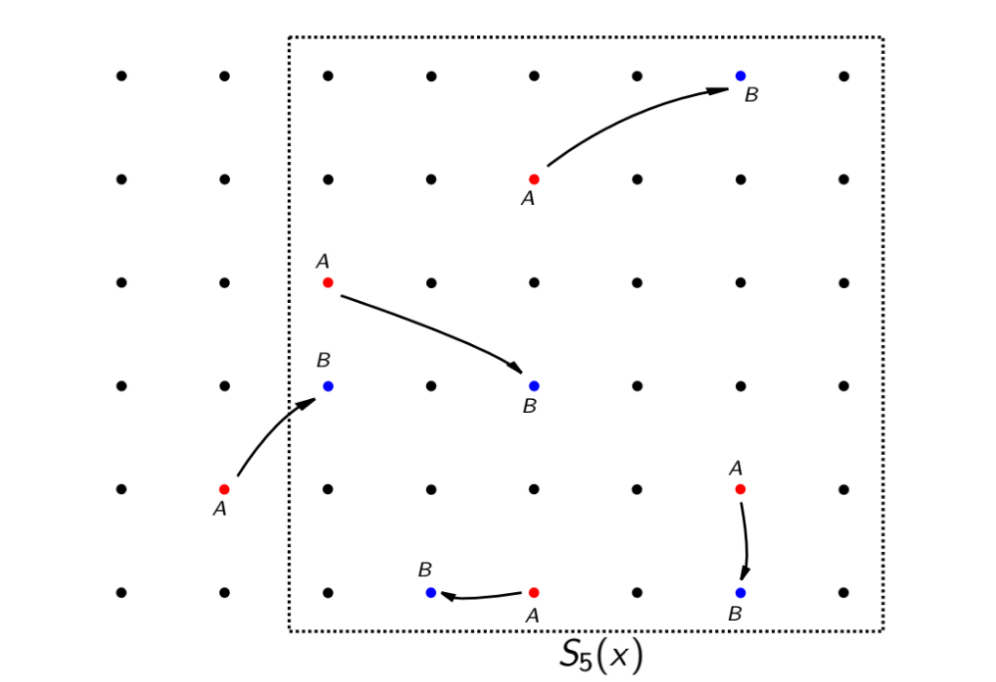
\includegraphics[width=.62\linewidth]{figures/N-20221214/11-discrepancy-box.png}
\caption{A finite orbit box $S_N(x)$; discrepancy compares observed counts with expected measure.}
\end{figure}

The key lemma states that there exist $\varepsilon>0$ and $M$ such that for all $x$ and $N$,
\[
  \left||S_N(x)\cap A|-\lambda(A)N^d\right|
  \le MN^{d-1-\varepsilon},
\]
and similarly for $B$:
\[
  \left||S_N(x)\cap B|-\lambda(B)N^d\right|
  \le MN^{d-1-\varepsilon}.
\]
Since $\lambda(A)=\lambda(B)$, large boxes contain nearly equal numbers of $A$ and $B$ points.  The error term grows more slowly than the volume term $N^d$, which is exactly what makes matching possible.

\section{From Laczkovich to Borel circle squaring}

Laczkovich's original proof used the axiom of choice.  Later work by Marks and Unger showed that the pieces can be chosen Borel.  This is much stronger: the pieces are still extremely complicated, but they are definable in the Borel hierarchy.

\begin{figure}[H]
\centering
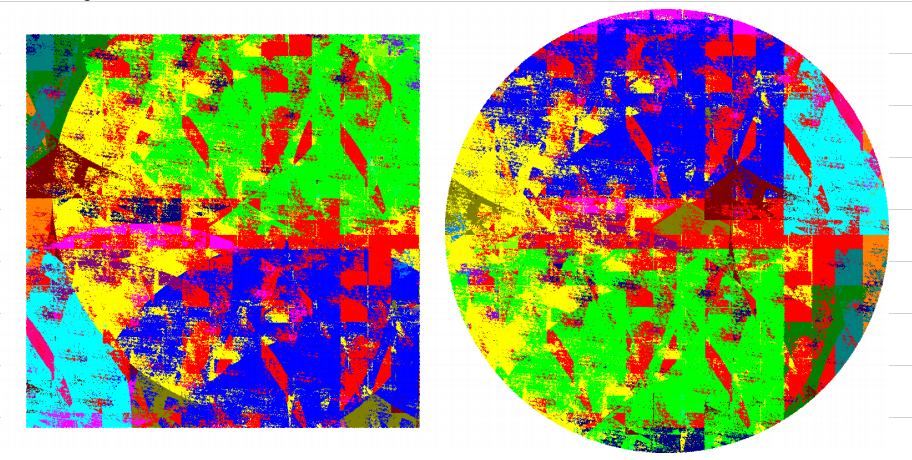
\includegraphics[width=.60\linewidth]{figures/N-20221214/12-borel-colored-partition.png}
\caption{A visual impression of the Borel circle-squaring pieces.}
\end{figure}

The final handwritten note says the main components are: Dehn invariant, group action, torus embedding, traversal/matching, and measure/discrepancy theory.  That summary is accurate.  The proof is not one trick; it is a combination of several fields.

\section{Expanded synthesis and advanced context}

The same question changes answer depending on the category of pieces.  Plane polygons are controlled by area.  Three-dimensional polyhedra require the Dehn invariant.  Tame planar scissors pieces preserve circular-boundary data, so a disk cannot become a square.  But arbitrary or Borel pieces are flexible enough for Laczkovich's theorem and Borel circle squaring.

Thus Tarski's circle-squaring problem is a crossroads of geometry, measure theory, group actions, discrepancy estimates, graph matching, and descriptive set theory.  The important lesson is not only that the answer is yes, but why the yes lives far beyond ordinary scissors geometry.


\paragraph{Expanded synthesis.}
The elementary geometric content of this chapter should be read through transformations and invariants. The earlier sections (`The route of the note`, `Equidecomposability and dissection congruence`, `Hilbert's third problem and the Dehn invariant`, `Measure-theoretic background`, `Tarski's circle-squaring problem`) may use coordinates, angles, determinants, parametrizations, or integral formulas, but the organizing question is: which quantities survive the transformations naturally associated with the problem? Euclidean geometry preserves distances and angles; affine geometry preserves lines and ratios on a line; projective geometry preserves incidence and cross ratio; differential geometry preserves coordinate-independent objects such as forms, metrics, and orientations.

This perspective separates different layers of a problem. A dot product belongs to metric geometry. A determinant belongs to oriented volume. A cross ratio belongs to projective geometry. A line or surface integral of a differential form belongs to oriented topology. A scalar area integral belongs to the metric-induced measure. Confusing these layers is the source of many errors, especially in vector calculus where $dS$, $F\cdot n\,dS$, $dx\wedge dy$, and boundary orientation look similar but encode different structures.

When returning to the original examples, identify the natural object before computing. If the problem is about concurrence or collinearity, projective or affine tools may be natural. If it is about distance, angle, or orthogonality, metric tools are essential. If it is about flux or circulation, differential forms and orientation explain the signs. The advanced viewpoint makes the elementary solution more disciplined rather than more abstract for its own sake.

\notechapter{N-20230801}{Reading Hitchin: Self-Duality Equations, Higgs Bundles, and Geometric Structures}

\section{Starting point}

This note is a reading reconstruction around Hitchin's paper on the self-duality equations on a Riemann surface.  The main mathematical movement is a dimensional reduction from four-dimensional self-dual Yang--Mills theory to equations on a Riemann surface, producing what are now called Hitchin equations.

Let \(\Sigma\) be a compact Riemann surface, \(E\to\Sigma\) a complex vector bundle, \(A\) a connection, and \(\Phi\) a Higgs field, locally an \(\operatorname{End}(E)\)-valued \((1,0)\)-form.  The Hitchin equations have the schematic form
\[
  F_A+[\Phi,\Phi^*]=0,
  \qquad
  \bar\partial_A\Phi=0.
\]
Here \(F_A\) is the curvature of \(A\), and \(\Phi^*\) is the adjoint of the Higgs field with respect to a Hermitian metric.

\section{Connections and curvature}

A connection \(A\) is a way of differentiating sections of a bundle.  Its curvature is
\[
  F_A=dA+A\wedge A,
\]
which measures the failure of covariant derivatives to commute.  Gauge transformations act on connections, and the equations are considered modulo this gauge symmetry.

\begin{remark}
This already explains why the moduli space is not just a solution set.  One must divide by gauge equivalence, so the actual object is a quotient, often with singularities and rich geometric structure.
\end{remark}

\section{Higgs bundles}

A Higgs bundle over a Riemann surface is roughly a pair
\[
  (E,\Phi),
\]
where \(E\) is a holomorphic vector bundle and
\[
  \Phi:E\to E\otimes K_\Sigma
\]
is a holomorphic \(K_\Sigma\)-twisted endomorphism.  The field \(\Phi\) is the Higgs field.

The equation
\[
  \bar\partial_A\Phi=0
\]
says that \(\Phi\) is holomorphic with respect to the holomorphic structure determined by \(A\).

\section{The moduli space}

The moduli space of solutions to Hitchin's equations is deeply structured.  It carries a hyperkähler metric and admits several interpretations:
\begin{enumerate}[(i)]
  \item as a moduli space of solutions to gauge-theoretic PDEs;
  \item as a moduli space of stable Higgs bundles;
  \item as a moduli space of flat connections or representations of the fundamental group.
\end{enumerate}

This is the beginning of non-abelian Hodge theory.  In rank one, Hodge theory relates differential forms, cohomology, and harmonic representatives.  In higher rank, the analogous story involves Higgs bundles, flat connections, and representations.

\section{The Hitchin fibration}

The characteristic polynomial of the Higgs field gives invariant functions.  For example, in rank \(n\), one considers
\[
  \operatorname{tr}(\Phi),\quad \operatorname{tr}(\Phi^2),\quad \ldots,\quad \operatorname{tr}(\Phi^n).
\]
These define the Hitchin map from the moduli space of Higgs bundles to an affine space of differentials, often called the Hitchin base.

The generic fibers are abelian varieties, related to spectral curves.  Thus the Hitchin system is an algebraically completely integrable system.

\section{Spectral curves}

The spectral curve is defined by the eigenvalue equation of the Higgs field.  Informally, if \(\lambda\) denotes a coordinate on the cotangent direction, then the spectral curve is given by
\[
  \det(\lambda-\Phi)=0.
\]
It lives inside the total space of the canonical bundle \(K_\Sigma\).  A Higgs bundle can often be reconstructed from line bundle data on its spectral curve.

\begin{remark}
This is one of the most attractive parts of the theory: a nonabelian problem about vector bundles and Higgs fields is transformed into abelian geometry on a spectral curve.
\end{remark}

A concrete rank-two model makes the slogan much less vague.  I take \(\Sigma\) to be the genus-two hyperelliptic curve
\[
  \Sigma:\quad y^2=(x^2-1)(x^2-4)(x^2-9).
\]
This is the promised genus-two surface in a form one can calculate with.  I deliberately do not call it an elliptic curve or a one-dimensional complex torus, since those have genus one.  A basis of holomorphic one-forms is
\[
  \omega_0=\frac{dx}{y},\qquad \omega_1=x\frac{dx}{y}.
\]
Now set
\[
  E=\mathcal O_\Sigma\oplus\mathcal O_\Sigma
\]
and choose a local coordinate \(z\) so that quadratic differentials are written as \(Q(z)\,dz^2\).  In companion-matrix form a rank-two Higgs field may be written locally as
\[
  \Phi=
  \begin{pmatrix}
    0&1\\
    -Q_2&-Q_1
  \end{pmatrix}dz,
\]
where \(q_1=Q_1dz\in H^0(K)\) and \(q_2=Q_2dz^2\in H^0(K^2)\).  For the simplest trace-free calculation I put \(q_1=0\) and choose the explicit holomorphic quadratic differential
\[
  q_2=(x^2-2)\left(\frac{dx}{y}\right)^2\in H^0(\Sigma,K^2).
\]
The zeros occur at \(x=\pm\sqrt2\).  Since these are not branch values of the hyperelliptic map, each value of \(x\) gives two points of \(\Sigma\), so \(q_2\) has four simple zeros, exactly as \(\deg K^2=4g-4=4\) predicts for \(g=2\).

The characteristic equation is now just a two-by-two determinant:
\[
\begin{aligned}
  \det(\lambda I-\Phi)
  &=
  \det
  \begin{pmatrix}
    \lambda&-1\\
    Q_2&\lambda+Q_1
  \end{pmatrix}dz^2  \\
  &=\lambda^2+q_1\lambda+q_2.
\end{aligned}
\]
With \(q_1=0\), the spectral curve \(\widetilde\Sigma\subset\operatorname{Tot}(K)\) is therefore
\[
  \eta^2+q_2=0,
\]
where \(\eta\) is the tautological one-form on the total space of \(K\).  Equivalently, after absorbing the harmless sign into the name of \(q_2\), one writes the same calculation as \(\eta^2=q_2(z)\).  The projection
\[
  \pi:\widetilde\Sigma\to\Sigma
\]
is a double cover, branched over the four zeros of \(q_2\).  Riemann--Hurwitz gives
\[
  2g(\widetilde\Sigma)-2
  =2(2g(\Sigma)-2)+4
  =2\cdot2+4=8,
\]
so \(g(\widetilde\Sigma)=5\).

The reconstruction is also concrete.  If \(\mathcal L\) is a line bundle on the spectral curve, then
\[
  E=\pi_*\mathcal L.
\]
Multiplication by the tautological eigenvalue \(\eta\) gives
\[
  \mathcal L\longrightarrow \mathcal L\otimes \pi^*K,
\]
and after applying \(\pi_*\) this becomes
\[
  \Phi:E=\pi_*\mathcal L\longrightarrow \pi_*(\mathcal L\otimes\pi^*K)
  \cong E\otimes K.
\]
Thus the Higgs field is literally multiplication by the coordinate on the spectral cover.  In the trace-free, fixed-determinant version relevant to this example, the Hitchin base is
\[
  H^0(K^2),\qquad \dim H^0(K^2)=3g-3=3,
\]
and the generic fiber is the Prym variety
\[
  \operatorname{Prym}(\widetilde\Sigma/\Sigma)
  =\ker\!\left(\operatorname{Nm}:\operatorname{Jac}(\widetilde\Sigma)\to\operatorname{Jac}(\Sigma)\right)^0.
\]
If the determinant condition is removed one gets the full Jacobian of the spectral curve instead.  This distinction is worth keeping: ``abelian variety'' is the broad slogan, while ``Prym'' is the sharper answer in the fixed-determinant rank-two case.

\section{Geometric Langlands perspective}

Hitchin moduli spaces appear naturally in the geometric Langlands program.  The Hitchin fibration organizes the moduli space into a structure where duality phenomena become visible.  Mirror symmetry for Hitchin systems is one of the bridges between gauge theory, algebraic geometry, and representation theory.

\section{Synthesis}

Hitchin's equations sit at a crossroads:
\[
\begin{gathered}
  \text{gauge theory}\quad \text{Riemann surfaces}\quad \text{Higgs bundles}\\
  \text{integrable systems}\quad \text{geometric Langlands}.
\end{gathered}
\]
The central idea is that reducing self-duality equations to a Riemann surface produces Hitchin's equations.  Their moduli space remembers differential-geometric structure on one side and algebraic-geometric structure on the other.


\section{Moment-map reading of the equations}

A useful way to read Hitchin's equations is through symplectic reduction.  The space of pairs \((A,\Phi)\) is infinite-dimensional, and the unitary gauge group acts on it.  The curvature equation
\[
  F_A+[\Phi,\Phi^*]=0
\]
can be interpreted as a zero moment-map condition for this action.

This viewpoint explains why stability appears.  In many moduli problems, solving a differential equation modulo a compact group is equivalent to imposing an algebraic stability condition modulo a complexified group.  For Higgs bundles, this is the Hitchin--Kobayashi style bridge.

\section{Spectral curves as global eigenvalues}

For a single matrix, eigenvalues are roots of its characteristic polynomial.  A Higgs field is a matrix-valued one-form varying over \(\Sigma\).  The spectral curve is the global version of taking eigenvalues:
\[
  \det(\lambda-\Phi)=0.
\]
It lives in the total space of the canonical bundle.  Over a generic point of \(\Sigma\), it records eigenvalues of \(\Phi\); globally, these eigenvalues form a branched cover.

This is why the Hitchin fibration is powerful.  The complicated nonabelian data of a Higgs bundle can often be transformed into abelian data: a line bundle on the spectral curve.

\section{Four descriptions to keep together}

The reader should keep four translations active:
\[
  \text{PDE solution}\leftrightarrow \text{stable Higgs bundle}
  \leftrightarrow \text{flat connection}
  \leftrightarrow \text{representation of }\pi_1(\Sigma).
\]
The difficulty of Hitchin's theory is precisely that none of these descriptions is disposable.  The equations are analytic, the moduli problem is algebraic, the spectral curve is geometric, and the flat connection is representation-theoretic.

\section{Source repair: Yang--Mills background}

The uploaded version begins from Yang--Mills theory.  Let \(P\) be a principal \(G\)-bundle over a compact manifold \(M\), and let \(A\) be a connection.  Locally, \(A\) is a Lie-algebra-valued one-form, and its curvature is
\[
  F_A=dA+\frac12[A,A].
\]
The Yang--Mills functional is
\[
  S_{YM}(A)=\int_M \operatorname{tr}(F_A\wedge *F_A).
\]
Its Euler--Lagrange equation is
\[
  d_A *F_A=0.
\]

In four dimensions, two-forms decompose into self-dual and anti-self-dual parts:
\[
  \omega=\omega^++\omega^- ,\qquad *\omega^\pm=\pm\omega^\pm.
\]
A self-dual connection satisfies
\[
  F_A=*F_A.
\]
Such a connection automatically solves the Yang--Mills equation.  This is the four-dimensional origin of the Hitchin system.

\section{Source repair: dimensional reduction}

Hitchin's equations can be understood as a dimensional reduction of the four-dimensional self-duality equations.  Roughly, one splits the four-dimensional geometry into a two-dimensional Riemann surface direction and two suppressed directions.  Components of the original connection in the suppressed directions become a Higgs field.

The resulting equations on a Riemann surface \(\Sigma\) are
\[
  F_A+[\Phi,\Phi^*]=0,
  \qquad
  \bar\partial_A\Phi=0.
\]
Here \(A\) is a connection on a bundle over \(\Sigma\), \(\Phi\) is an \(\operatorname{End}(E)\otimes K\)-valued Higgs field, and \(K\) is the canonical bundle.

The uploaded note emphasizes that \(\Phi\) is not an arbitrary extra variable.  It is the remnant of the higher-dimensional connection after reduction.

\section{Source repair: gauge invariance}

Under a gauge transformation \(g\), the Higgs field transforms as
\[
  \Phi\mapsto g\Phi g^{-1},\qquad
  \Phi^*\mapsto g\Phi^*g^{-1}.
\]
Therefore
\[
  [\Phi,\Phi^*]\mapsto g[\Phi,\Phi^*]g^{-1}.
\]
This explains why the bracket term is globally meaningful and compatible with quotienting by the gauge group.  The curvature term transforms in the same conjugation pattern, so the first Hitchin equation is gauge invariant.

\section{Source repair: Higgs bundles and stability}

A Higgs bundle is a pair
\[
  (E,\Phi),\qquad \Phi\in H^0(\Sigma,\operatorname{End}(E)\otimes K).
\]
Stability is measured by slope:
\[
  \mu(E)=\frac{\deg E}{\operatorname{rank}E}.
\]
For an ordinary vector bundle, stability asks that every proper nonzero subbundle \(F\subset E\) have
\[
  \mu(F)<\mu(E).
\]
For Higgs bundles one restricts to \(\Phi\)-invariant subbundles.  This condition is essential because the moduli space behaves well only after excluding unstable objects.

This is the algebraic-geometric side of the Hitchin--Kobayashi philosophy: solving differential equations modulo unitary gauge transformations corresponds to imposing stability modulo complex gauge transformations.

\section{Source repair: spectral data and Hitchin fibration}

The spectral curve is defined by the characteristic polynomial of the Higgs field:
\[
  \det(\lambda I-\Phi)=\lambda^n+a_1\lambda^{n-1}+\cdots+a_n=0.
\]
The coefficients \(a_i\) are sections of powers of the canonical bundle.  This gives the Hitchin map
\[
  h:\mathcal M\to \bigoplus_{i=1}^n H^0(\Sigma,K^i).
\]
For a generic spectral curve, the fiber of this map is an abelian variety; in the rank-two fixed-determinant case above it is more precisely a Prym variety, while in the unconstrained \(GL_2\) version it is the Jacobian of the spectral curve.

This is the mechanism by which a nonabelian moduli problem becomes an algebraically completely integrable system.  The base records eigenvalue-like data; the fiber records line-bundle-like data on the spectral curve.

\section{Source repair: geometric Langlands and S-duality}

The uploaded note connects Hitchin systems to geometric Langlands.  The rough slogan is that local systems for the Langlands dual group \({}^LG\) correspond to sheaf-theoretic automorphic data on the moduli of \(G\)-bundles.

Hitchin moduli spaces provide the geometric stage on which this duality becomes visible.  In the physical picture developed by Kapustin and Witten, S-duality in four-dimensional supersymmetric Yang--Mills theory becomes a geometric Langlands duality after reduction.  Hitchin's equations are the bridge between the gauge-theoretic and algebro-geometric languages.

\section{Source repair: local work still missing}

The uploaded text names the right objects, but several parts still need to be made local and computable before the story is really understood.
\begin{enumerate}[(i)]
  \item In a local holomorphic coordinate \(z\), Hitchin's equations should be written in terms of a connection form, a Higgs field \(\varphi\,dz\), and the adjoint \(\varphi^*\,d\bar z\).  Without this coordinate calculation, the equation \(F_A+[\varphi,\varphi^*]=0\) remains only symbolic.
  \item The tangent space to the moduli problem is controlled by a deformation complex.  The missing calculation is to identify infinitesimal gauge transformations, infinitesimal deformations of \((A,\varphi)\), and the linearized equations in one complex.
  \item Stability is not just a label attached to Higgs bundles.  It is the condition that removes bad orbit-closure behavior, so it is the algebro-geometric replacement for asking the gauge quotient to have reasonable points.
  \item The spectral curve construction should be checked in low rank by writing
  \[
    \det(\eta-\\varphi)=0
  \]
  inside the total space of the canonical bundle.  This makes the Hitchin base concrete: its coordinates are the coefficients of the characteristic polynomial.
\end{enumerate}

A good next pass through this topic should therefore not try to memorize the whole nonabelian Hodge correspondence at once.  It should work through one rank-two example, compute the characteristic polynomial of a Higgs field, locate the spectral curve, and then match the deformation complex with the expected dimension of the moduli space.

\include{tex/notes/N-20250705}
\include{tex/notes/N-20250707}


\part{Machine Learning and Inference}
\label{vol:16-machine-learning-and-inference}
\begingroup
\small
\sloppy
\parttoc
\endgroup

% This file is generated during volume reorganization.
% Volume: Machine Learning and Inference

\notechapter{N-20250926}{Backpropagation in One MLP Layer: From a Three-Dimensional Tensor to an Outer Product}

\section{The setting}

Consider one middle layer of a multilayer perceptron:
\[
  z=Wx+b,\qquad y=\sigma(z).
\]
Here
\[
  x\in\mathbb R^n,\qquad
  W\in\mathbb R^{m\times n},\qquad
  b\in\mathbb R^m,\qquad
  z,y\in\mathbb R^m.
\]
The activation function $\sigma$ acts elementwise, for example sigmoid or ReLU.  The goal of backpropagation is to compute
\[
  \frac{\partial L}{\partial W}
\]
for a loss function $L$.

The note uses the common softmax--cross-entropy setting as motivation.  If the final layer produces logits $z_i$, then
\[
  \hat y_i=\frac{e^{z_i}}{\sum_j e^{z_j}},\qquad
  L=-\sum_i t_i\ln \hat y_i,
\]
where $t_i$ is a one-hot label.  Backpropagation asks how this scalar loss changes when each weight $W_{j,k}$ changes.

\section{The theoretical tensor}

Strictly speaking, the derivative of the vector $y\in\mathbb R^m$ with respect to the matrix $W\in\mathbb R^{m\times n}$ has three indices:
\[
  \frac{\partial y_i}{\partial W_{j,k}}.
\]
The index $i$ chooses the output component, $j$ chooses the row of $W$, and $k$ chooses the column of $W$.  So the object has shape
\[
  m\times m\times n.
\]

This is the source of the confusion recorded in the note.  The derivative is theoretically a third-order tensor, but in neural-network code one usually sees only a matrix gradient.  The matrix appears after chain-rule contraction with the upstream gradient.

\section{Computing the sparse derivative}

Write the linear preactivation component as
\[
  z_r=\sum_{t=1}^n W_{r,t}x_t+b_r.
\]
Then
\[
  \frac{\partial z_r}{\partial W_{j,k}}
  =
  \begin{cases}
  x_k,&r=j,\\
  0,&r\ne j,
  \end{cases}
  =\delta_{rj}x_k.
\]
This is sparse because $z_r$ depends only on row $r$ of $W$.

For $y_i=\sigma(z_i)$ with elementwise activation,
\[
  \frac{\partial y_i}{\partial z_r}=0\quad(i\ne r),\qquad
  \frac{\partial y_i}{\partial z_i}=\sigma'(z_i).
\]
Thus
\[
  \frac{\partial y_i}{\partial W_{j,k}}
  =\sum_{r=1}^m
  \frac{\partial y_i}{\partial z_r}
  \frac{\partial z_r}{\partial W_{j,k}}
  =\frac{\partial y_i}{\partial z_j}x_k.
\]
For elementwise activation this is nonzero only when $i=j$.

\section{Contraction by the chain rule}

The loss $L$ is scalar.  Therefore
\[
  \frac{\partial L}{\partial W_{j,k}}
  =\sum_{i=1}^m
  \frac{\partial L}{\partial y_i}
  \frac{\partial y_i}{\partial W_{j,k}}.
\]
Substituting the previous formula gives
\[
  \frac{\partial L}{\partial W_{j,k}}
  =\sum_{i=1}^m
  \frac{\partial L}{\partial y_i}
  \frac{\partial y_i}{\partial z_j}x_k.
\]
The sum over $i$ is exactly the $j$-th component of the upstream gradient with respect to $z$:
\[
  \delta_j=\frac{\partial L}{\partial z_j}.
\]
Hence
\[
  \frac{\partial L}{\partial W_{j,k}}=\delta_jx_k.
\]
Stacking all $j,k$ gives the outer product
\[
  \boxed{\displaystyle
  \frac{\partial L}{\partial W}=\delta x^T
  }
\]
where
\[
  \delta=\frac{\partial L}{\partial z}.
\]

\section{Why the tensor disappears}

The original derivative $\partial y/\partial W$ is a tensor with shape $(m,m,n)$.  But backpropagation does not need to store it.  The chain rule contracts it with the vector $\partial L/\partial y$, leaving a matrix of shape $(m,n)$.

In the note's language:
\[
  \text{three-dimensional tensor}
  \quad\xrightarrow{\text{chain-rule summation}}
  \quad
  \text{matrix gradient}.
\]
This is not a loss of information for gradient descent, because gradient descent only needs the derivative of the scalar loss with respect to each parameter.

\section{Contravariant reading of the same calculation}

The same computation can be described as a pullback of covectors.  A forward layer is a map
\[
  f:\text{parameters and activations}\longrightarrow \text{outputs}.
\]
Its differential sends small forward perturbations to small output perturbations:
\[
  df:T_xX\to T_{f(x)}Y.
\]
But the loss supplies a covector at the output,
\[
  dL\in T_{f(x)}^*Y,
\]
and backpropagation sends it backward by precomposition:
\[
  f^*(dL)=dL\circ df\in T_x^*X.
\]
This is why reverse-mode differentiation is naturally contravariant.

For a batched linear layer in PyTorch convention,
\[
  X\in\mathbb R^{b\times n},\qquad
  W\in\mathbb R^{m\times n},\qquad
  Y=XW^T\in\mathbb R^{b\times m},
\]
the component formula is
\[
  Y_{\alpha i}=\sum_{k=1}^n X_{\alpha k}W_{ik}.
\]
Hence
\[
  \frac{\partial Y_{\alpha i}}{\partial W_{jk}}
  =
  \delta_{ij}X_{\alpha k},
\]
a Jacobian tensor of shape \((b,m,m,n)\).  Contracting with the upstream gradient \(G=\partial L/\partial Y\), of shape \((b,m)\), gives
\[
\begin{aligned}
  \frac{\partial L}{\partial W_{jk}}
  &=
  \sum_{\alpha,i}G_{\alpha i}
  \frac{\partial Y_{\alpha i}}{\partial W_{jk}}\\
  &=
  \sum_{\alpha}G_{\alpha j}X_{\alpha k},
\end{aligned}
\]
so
\[
  \frac{\partial L}{\partial W}=G^TX.
\]
If the weights are stored instead as \(W_{\mathrm{col}}\in\mathbb R^{n\times m}\) and \(Y=XW_{\mathrm{col}}\), the same formula appears as
\[
  \frac{\partial L}{\partial W_{\mathrm{col}}}=X^TG.
\]
The two expressions differ only by the convention for storing the weight matrix.

\section{Outer-product expression}

Let
\[
  \frac{\partial y}{\partial z}
\]
be treated as a column vector for elementwise activation, with entries $\sigma'(z_i)$.  Then the derivative of $y$ with respect to $W$ can be represented row by row as
\[
  \frac{\partial y}{\partial W}\sim
  \begin{bmatrix}
  \frac{\partial y_1}{\partial z_1}x^T\\
  \frac{\partial y_2}{\partial z_2}x^T\\
  \vdots\\
  \frac{\partial y_m}{\partial z_m}x^T
  \end{bmatrix}
  =\left(\frac{\partial y}{\partial z}\right)x^T.
\]
For the scalar loss, replace $\partial y/\partial z$ by the backpropagated vector $\delta=\partial L/\partial z$.

\section{Numerical example}

The note gives a simple example with
\[
  m=2,\qquad n=3,\qquad x=[1,2,3]^T,\qquad z=[0.1,-1.0]^T.
\]
For sigmoid,
\[
  \sigma'(0.1)\approx0.2494,\qquad
  \sigma'(-1.0)\approx0.1966.
\]
Therefore
\[
  \frac{\partial y}{\partial W}\sim
  \begin{bmatrix}0.2494\\0.1966\end{bmatrix}
  \begin{bmatrix}1&2&3\end{bmatrix}
  =
  \begin{bmatrix}
  0.2494&0.4988&0.7482\\
  0.1966&0.3932&0.5898
  \end{bmatrix}.
\]
Each row is the input vector scaled by the derivative of the corresponding output.

\section{Einstein notation proof}

The handwritten proof uses indices.  Let $y=f(z)$ and $z=Wx$.  For a matrix entry $A_{pq}=W_{pq}$,
\[
  \frac{\partial z_i}{\partial A_{pq}}
  =\frac{\partial}{\partial A_{pq}}
  \sum_j A_{ij}x_j
  =\delta_{ip}x_q.
\]
Then
\[
  \frac{\partial L}{\partial A_{pq} }
  =\sum_i \frac{\partial L}{\partial y_i}
  \frac{\partial y_i}{\partial z_p}x_q.
\]
For elementwise activation, this becomes
\[
  \frac{\partial L}{\partial A_{pq}}
  =\frac{\partial L}{\partial z_p}x_q.
\]
This is the component form of $\partial L/\partial W=\delta x^T$.

\section{Kronecker product viewpoint}

The note also explores vectorization.  If $y=f(Wx)$ and we vectorize $W$, then the Jacobian with respect to $\operatorname{vec}(W)$ can be written using Kronecker products.  The important identity is that changing one matrix entry affects only one row of $z$, which is encoded by a Kronecker delta.

In batch form, if $X$ is a matrix of inputs and $\Delta$ is the matrix of upstream gradients, then the gradient becomes
\[
  \frac{\partial L}{\partial W}=\Delta X^T.
\]
This is the same outer-product rule, summed over the batch dimension.

\section{Softmax--cross-entropy simplification}

For the final layer with softmax and cross entropy, the derivative simplifies to
\[
  \frac{\partial L}{\partial z}=\hat y-t.
\]
Therefore the final-layer weight gradient is
\[
  \frac{\partial L}{\partial W}=(\hat y-t)x^T.
\]
This is why implementation code often looks much simpler than the theoretical tensor derivation.

\section{A wider interpretation}

The key lesson is that matrix calculus is compressed tensor calculus.  The full derivative of a vector with respect to a matrix is a higher-order object, but backpropagation contracts it immediately with an upstream gradient.  The result is an outer product: error signal times input.  This is the local rule behind every dense neural-network layer.


\paragraph{Expanded synthesis.}
For this chapter, the elementary material should be read as a study of what remains invariant when coordinates change. The earlier sections (`The setting`, `The theoretical tensor`, `Computing the sparse derivative`, `Contraction by the chain rule`, `Why the tensor disappears`) compute with arrays, bases, pivots, determinants, or eigenvectors; the deeper object is a linear map together with the spaces it acts on. A matrix is a representation of that map after bases have been chosen. This is why formulas such as
\[
  A' = P^{-1}AP,\qquad \widetilde A = T^{-1}AS
\]
are not cosmetic: they distinguish an intrinsic morphism from a coordinate description.

The structural hierarchy is as follows. Kernels record what a map forgets, images record what it reaches, cokernels record obstructions to solvability, and quotients record information after an equivalence has been imposed. Determinants act on the top exterior power and therefore measure oriented volume; traces are invariant under cyclic rearrangement and become characters in representation theory; adjoints depend on an inner product and lead to self-adjoint spectral theory.

A useful way to return to the computations is to ask, for every formula, which invariant it is measuring. Row reduction measures rank and kernel; diagonalization measures decomposition into invariant subspaces; Gram--Schmidt measures orthogonal projection; positive definiteness measures ellipsoid geometry; tensor notation measures how components transform. The elementary methods are therefore the finite-dimensional laboratory in which duality, quotienting, functoriality, and spectral decomposition can be seen clearly.

\include{tex/notes/N-20251008}
\include{tex/notes/N-20251009}
\include{tex/notes/N-20251010}
\include{tex/notes/N-20251011}
\include{tex/notes/N-20260302}

